\documentclass[ruled,graybox]{svmult}
%\usepackage{mathptmx}        % selects Times Roman as basic font
%\usepackage{helvet}          % selects Helvetica as sans-serif font
%\usepackage{courier}         % selects Courier as typewriter font

\usepackage[document]{ragged2e}

\usepackage{graphicx,color}
\usepackage{amsmath, amssymb}
%\usepackage[ruled]{algorithm}
\usepackage{algorithmic}
\usepackage{url}

% TODO marker
\usepackage{color}
\usepackage{xspace}
\definecolor{ScarletRed}{rgb}{0.80,0.00,0.00}
\newcommand\todo[1]{\textcolor{ScarletRed}{\textbf{\colorbox{yellow}{\small TODO:}} [\emph{#1}]}\xspace}

\setcounter{secnumdepth}{3}

\frontmatter
\mainmatter
\backmatter


\begin{document}



\frontmatter%%%%%%%%%%%%%%%%%%%%%%%%%%%%%%%%%%%%%%%%%%%%%%%%%%%%%%
%\include{dedic}


\thispagestyle{empty}
\providecommand\pdfbookmark[3][]{} \pdfbookmark[0]{Title Page}{bm:Title}
\vspace*{1cm}
\vfill
\begin{center}
\textsc{\huge{Introduction to Computational Intelligence}}\\
\vfill
Editors\\[\baselineskip]
\textsc{\Large{Leandro L. Minku, George Cabral, Marcella Martins, Markus Wagner}}
\vfill
\end{center}
\begin{figure}[ht!]
\centering

\includegraphics[height=1.5cm]{ieee-logo.png}
\hspace{0.5cm}

\includegraphics[height=1.5cm]{ieee-cis-logo.jpg}
\end{figure}
\begin{center}
% Cold Atoms Research Group\\[-0.8em]
An IEEE Computational Intelligence Society Open Book\\
DOI: 10.5281/zenodo.7537827\\[-0.8em]
\end{center}
%\copyright\ Copyright by \MakeUppercase{\@Author},~\@Year\\
%All Rights Reserved
\clearpage


%%%%%%%%%%%%%%%%%%%%%%foreword.tex%%%%%%%%%%%%%%%%%%%%%%%%%%%
% sample foreword
%
% Use this file as a template for your own input.
%
%%%%%%%%%%%%%%%%%%%%%%%% Springer %%%%%%%%%%%%%%%%%%%%%%%%%%

\foreword

Due to its power to solve large scale problems and analyse vast amounts of data that would be difficult or time consuming for humans to deal with manually, the field of Computational Intelligence has grown tremendously in importance over the past years. We nowadays see widespread use of computational intelligence in the most varied applications. A few examples include approaches to detect credit card fraud, recognise faces, transcribe voice to text, identify spam, route and schedule deliveries, design aerodynamic high speed trains, etc. 

It is thus not surprising that we see a growing number of people who are keen to learn about this field. However, there is a lack of open resources that combine several different types of computational intelligence approaches in one place, so that people can easily get an introduction to this field. People eager to learn about computational intelligence may also struggle to get help from others when trying to understand existing approaches. Those willing to start teaching about this topic may also struggle to find free resources to guide them. 

This \textit{open} book has been created as a community effort to overcome these issues. The notion of \textit{openness} of this book includes, but goes beyond open access. In addition to being available through an open license so that resources on computational intelligence are accessible to all, this book is hosted in github. Such initiative will enable the book to be continuously improved over time through pull requests to fix typos, add clarifications, add new exercises, add examples of open software code, add video lectures on the content, etc. Therefore, this book is \textit{open} for the community to propose enhancements over time. The book is also associated to github discussion boards, so that people can ask questions and the community can help with answering those questions, creating an \textit{open} community that all can join in. 

If you would like to propose an enhancement through a pull request to this book, we ask you to first contact the current chair of the IEEE Computational Intelligence Society Education Portal Subcommittee (\url{https://cis.ieee.org/}). The chair will advise you on how to proceed. Minor changes to existing chapters will be handled by the subcommittee directly, whereas the subcommittee will liaise with the original authors to obtain their consent for incorporating larger pull requests. 

We hope that you will find the book a useful resource to learn about computational intelligence.

\vspace{\baselineskip}
\begin{flushright}\noindent
Leandro L. Minku, George Cabral, Marcella Martins, Markus Wagner\\
IEEE CIS Computational Intelligence Open Book Editors -- First Edition 
\end{flushright}



%%%%%%%%%%%%%%%%%%%%%%foreword.tex%%%%%%%%%%%%%%%%%%%%%%%%%%%
% sample foreword
%
% Use this file as a template for your own input.
%
%%%%%%%%%%%%%%%%%%%%%%%% Springer %%%%%%%%%%%%%%%%%%%%%%%%%%

\preface

Due to its power to solve large scale problems and analyse vast amounts of data that would be difficult or time consuming for humans to deal with manually, the field of Computational Intelligence has grown tremendously in importance over the past years. We nowadays see widespread use of computational intelligence in the most varied applications. A few examples include approaches to detect credit card fraud, recognise faces, transcribe voice to text, identify spam, route and schedule deliveries, design aerodynamic high speed trains, etc. 

It is thus not surprising that we see a growing number of people who are keen to learn about this field. However, there is a lack of open resources that combine several different types of computational intelligence approaches in one place, so that people can easily get an introduction to this field. Those eager to learn about computational intelligence may also struggle to get help from others when trying to understand existing approaches, whereas those willing to start teaching this topic may struggle to find free resources to guide them. 

This \textit{open} book has been created as a community effort to overcome these issues. The notion of \textit{openness} of this book includes, but goes beyond open access. In addition to being available through an open license so that resources on computational intelligence are accessible to all, this book is hosted in github at:

\

\noindent \url{https://github.com/ieee-cis/IEEE-CIS-Open-Access-Book-Volume-1}. 

\

Such initiative will enable the book to be continuously improved over time through pull requests to fix typos, add clarifications, add new exercises, add examples of open software code, add video lectures on the content, etc. Therefore, this book is \textit{open} for the community to propose enhancements over time. The book is also associated to github discussion boards, so that people can ask questions and the community can help with answering those questions, creating an \textit{open} community that all can join in. 

If you would like to propose an enhancement through a pull request to this book, we ask you to first contact the current chair of the IEEE Computational Intelligence Society Education Portal Subcommittee (\url{https://cis.ieee.org/}). The chair will advise you on how to proceed. Minor changes to existing chapters will be handled by the subcommittee directly, whereas the subcommittee will liaise with the original authors to obtain their consent for incorporating larger pull requests. 

We thank all the authors who have contributed chapters to this book, all the anonymous reviewers who have reviewed the chapters, and all the community members who will contribute with this book and discussion boards in the future.

We hope that you will find the book a useful resource to learn about computational intelligence.

\vspace{\baselineskip}
\begin{flushright}\noindent
Leandro L. Minku, on behalf of the editors of the\\
IEEE CIS Computational Intelligence Open Book -- First Edition 
\end{flushright}



\abouteditors

\begin{center}
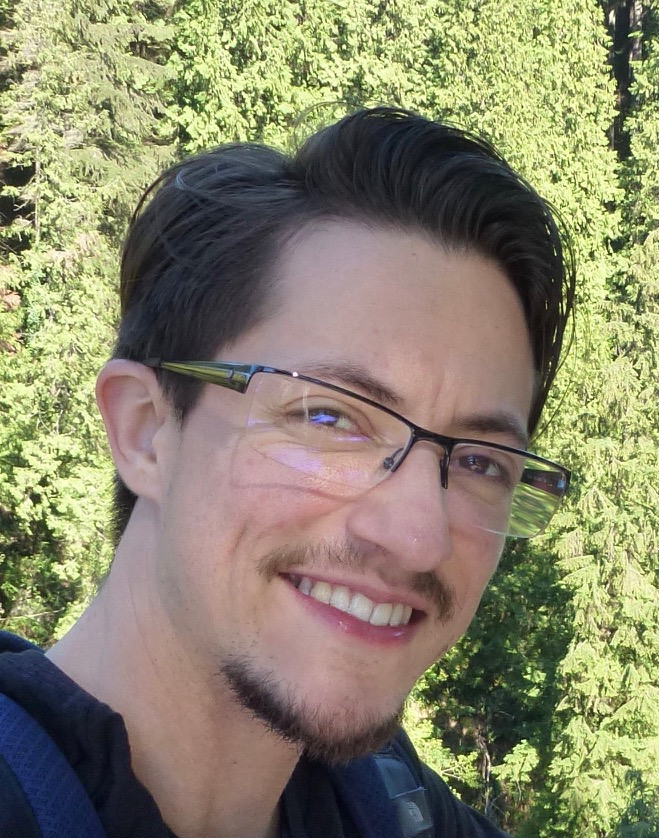
\includegraphics[width=.3\textwidth]{Photos/minku.jpg}
\end{center}

Dr. Leandro L. Minku is an Associate Professor at the School of Computer Science, University of Birmingham (UK). Prior to that, he was a Lecturer in Computer Science at the University of Leicester (UK). He received the PhD degree in Computer Science from the University of Birmingham (UK) in 2010. Dr. Minku's main research interests are machine learning in non-stationary environments / data stream mining, online class imbalance learning, ensembles of learning machines and computational intelligence for software engineering. His work has been published in internationally renowned journals such as IEEE Transactions on Neural Networks and Learning Systems, IEEE Transactions on Knowledge and Data Engineering, IEEE Transactions on Software Engineering and ACM Transactions on Software Engineering and Methodology. Among other roles, Dr. Minku is Associate Editor-in-Chief for Neurocomputing, Senior Editor for IEEE Transactions on Neural Networks and Learning Systems, and Associate Editor for Empirical Software Engineering Journal and Journal of Systems and Software. He was also the General Chair for the International Conference on Predictive Models and Data Analytics in Software Engineering (PROMISE 2019 and 2020), and Co-chair for the Artifacts Evaluation Track of the International Conference on Software Engineering (ICSE 2020).

\begin{center}
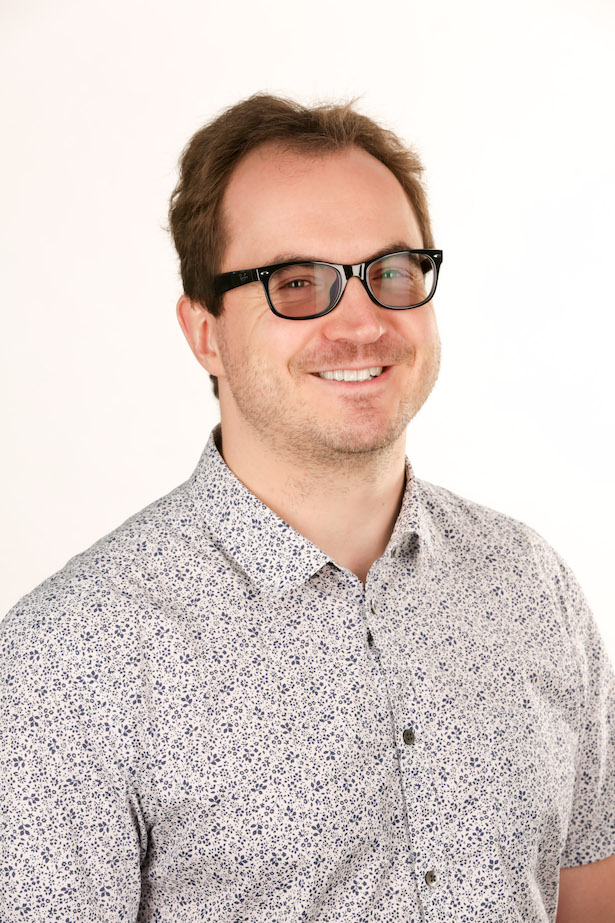
\includegraphics[width=.3\textwidth]{Photos/wagner.jpg}
\end{center}

Dr. Markus Wagner is an Associate Professor at Faculty of Information Technology, Monash University (Australia). He has done his PhD studies at the Max Planck Institute for Informatics in Saarbruecken, Germany and at the University of Adelaide, Australia. For the outcomes of his studies, he has received the university's Doctoral Research Medal --- the first for his school --- and three best paper awards. His research topics range from mathematical runtime analysis of heuristic optimisation algorithms and theory-guided algorithm design to applications of heuristic methods to renewable energy production, professional team cycling and software engineering. So far, he has been a program committee member 80+ times, and he has written 150+ articles with 200+ different co-authors. He has chaired several education-related committees within the IEEE CIS, where he also served as founding chair of two task forces. Markus is an ACM Lifetime Member, is on SIGEVO's Executive Board and serves as the first ever Sustainability Officer. He has contributed to GECCOs as Workshop Chair and Competition Chair, and most recently as General Chair.


\begin{center}
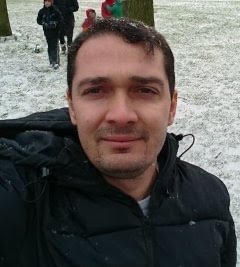
\includegraphics[width=.3\textwidth]{Photos/cabral.jpg}
\end{center}

Dr. George Cabral received his PhD degree from the Federal University of Pernambuco (Brazil) in 2014. His postdoc was conducted at the University of Birmingham (UK) in 2019. Currently, he is an adjunct professor at the Department of Computing at the Federal Rural University of Pernambuco (Brazil). He serves as reviewer for reputed journals such as Neurocomputing and Applied Software Computing. In addition, he has systematically served as committee member in prestigious conferences such as ICSE, ASE and ICONIP. His recent plublications include papers in reputed venues such as IEEE Transactions on Software Engineering and at the International Conference on Software Engineering (ICSE). He has taught courses involving Computational Intelligence for more than a decade and since 2020 he is applying this knowledge in practice for auditing public finances at the state of Pernambuco - Brazil. His research interests include Novelty Detection, One-class Classification, Data Mining, Class Imbalance Learning, Software Defect Prediction, Concept Drift, Online Learning, etc.

%\include{acknow}

\tableofcontents
\listoffigures

\mainmatter%%%%%%%%%%%%%%%%%%%%%%%%%%%%%%%%%%%%%%%%%%%%%%%%%%%%%%%
\title{History and Definitions of Computational Intelligence}
\author{}
\institute{}
\maketitle
\label{chp:history}
\label{chp:definitions}


Add your content here


\bibliographystyle{unsrt}
\bibliography{bibliography}

\title{History and Definitions of Computational Intelligence}
\author{}
\institute{}
\maketitle
\label{chp:history}
\label{chp:definitions}


Add your content here


\bibliographystyle{unsrt}
\bibliography{bibliography}



\part{Search-Based Optimization}
\label{prt:search-based-optimization}

\title{Local Search}
\label{chp:local-search}
\author{Sara Ceschia, Luca Di Gaspero, Andrea Schaerf}
\institute{DPIA, University of Udine\\ 
\texttt{\{sara.ceschia,luca.digaspero,andrea.schaerf\}@uniud.it}}
\maketitle


\emph{Local Search} is an algorithmic paradigm for combinatorial
search and optimization, which has been shown to be very effective for many
problems in the scientific literature. A large number
of techniques based on local search have been proposed to successfully
address a variety of practical problems.


Local search techniques belong to the larger class of the so-called
\emph{selective} methods that are based on the exploration of the
search space composed by complete solutions. This is opposed to
\emph{constructive} methods that build the solution in a step-by-step
manner by iteratively adding a new piece to the partial solution constructed
that far.  

In addition, local search techniques are non-exact, as they
do not guarantee to find the optimal solution. In the cases in which
the optimal solution is found, there is no way to prove that it is
indeed optimal, unless it has been established
with exact techniques that it is not possible to reach a value lower than that (i.e., it is a proven \emph{lower bound}).

Local search is based on the simple idea of \emph{navigating} the
search space by iteratively stepping from one state to one of its
\emph{neighbors}. The neighborhood of a state is the set of states
that can be obtained by applying a ``local change'' to it. The
definition of the neighborhood relation is dependent on the specific
problem under consideration, although there are some common
patterns that can be applied to search spaces with
similar structure.  The mechanism upon which the neighbor is selected
at each step is one of the main design choices that varies
among different local search techniques. In any case, this selection
mechanism relies upon the definition of the \emph{cost function} $F$,
which assesses the quality of each neighbor state, and it is also
problem dependent.

% NEW PARAGRAPH
Even though it is difficult to assess precisely when local search should be 
used instead of other optimization methods, a general observation is that 
its behavior depends on the landscape of the cost function. More precisely, if the 
landscape is relatively \emph{smooth} with respect to local 
changes, it is more likely that local search techniques will be successful.


In this chapter, we discuss the key elements of the local
search paradigm, which are independent of both the specific problem 
and the specific local search technique chosen to solve it.

We also introduce the basic local search techniques and discuss some
improvements and variations of such basic methods. We refer to
the following chapters %Chapter~\ref{cap:simulated-annealing} 
and the book by Hoos and St\"utzle \cite{HoSt05} for more complex local search
techniques. % others?



\section{Local Search Elements}

We first introduce one by one the key elements of local search.  In
detail, we will introduce the notions of \emph{search space},
\emph{neighborhood relation}, \emph{cost function}, \emph{initial
  solution selection}, \emph{move selection and acceptance criterion},
and \emph{stop criterion}.

\subsection{Search Space}

Given a search or optimization problem $P$ and an instance $I$ of $P$, we
associate to it a search space $S$, with the following properties:

\begin{itemize}
\item each element $s\in S$ represents a solution of $I$, not
  necessarily feasible (i.e., it might violate some constraint of the problem);
\item for search problems, at least one feasible solution of $I$ is
  represented in $S$;
\item for optimization problems, at least one optimal solution of $I$
  is represented in $S$.
\end{itemize}

If the previous requirements are met, we have a \emph{valid
  representation} of the problem. We refer to an element $s\in S$ as a
\emph{state}.

% Q: is n-queens already defined?
Consider for example the classical $n$-queens problem, which consists
in placing $n$ queens in an $n\times n$ chessboard so that they do not
attack each other neither vertically, nor horizontally, nor diagonally.

The direct representation of the problem would be with an $n\times n$
matrix of boolean-values, each representing the presence/absence of a
queen in the corresponding square. However, the intuitive search
spaces for local search already partition the chessboard in columns,
making use of $n$ integer-valued variables $\mathbf{x} = [x_1, x_2,
\dots, x_n]$ such that the assignment $x_i = j$ corresponds to place a
queen in position $(j,i)$ in the chessboard. Since this representation
places only one queen in each column, it implicitly provides against
vertical attacks.

There are two typical options for the definition of the
search space for the $n$-queens problem:

\begin{itemize}
\item \textbf{Assignment}: any variable $x_1,\dots, x_n$ can assume
  any value in the domain $\chi = \{1,\dots,n\}$. 
\item \textbf{Permutation}: variables can assume only distinct values in the domain $\chi = \{1,\dots,n\}$, resulting in a permutation of the numbers $1,\dots,n$. 
\end{itemize}

For example, $\mathbf{s_1} = [4,6,1,6,8,4,2,1]$ is a state for the instance with
$n = 8$ for \textbf{Assignment}, and $\mathbf{s_2} = [4,1,7,6,8,3,2,5]$ is a
state for both search spaces. These states are depicted in Figures~\ref{fig:nqueens-assignment} and \ref{fig:nqueens-permutation}.
% replace il the figure X with s_1 and s_2 (LUCA)

\begin{figure}
  \subfigures 
  \begin{minipage}{\textwidth}
    \leftfigure[t]{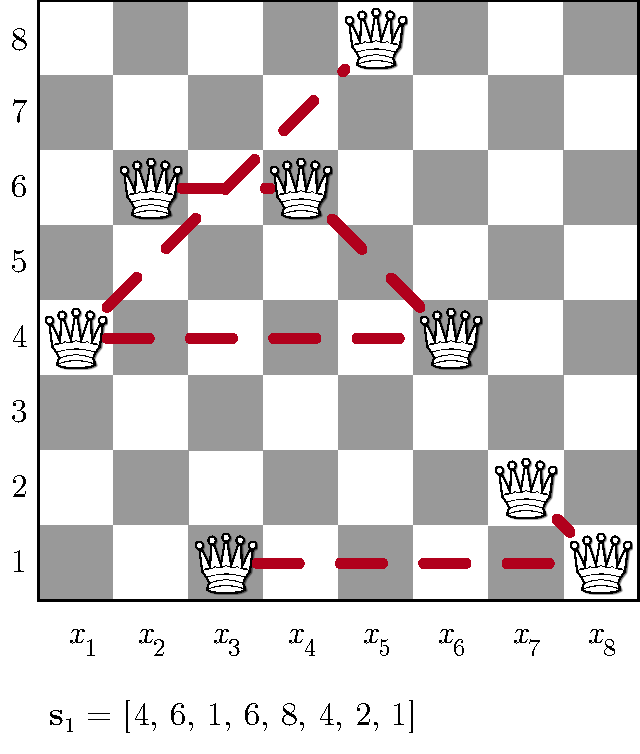
\includegraphics[width=0.4\textwidth]{"Part 2 - Search-Based Optimization/Local Search/n-queens/assignment.pdf"}}
    \hspace{\fill}
    \rightfigure[t]{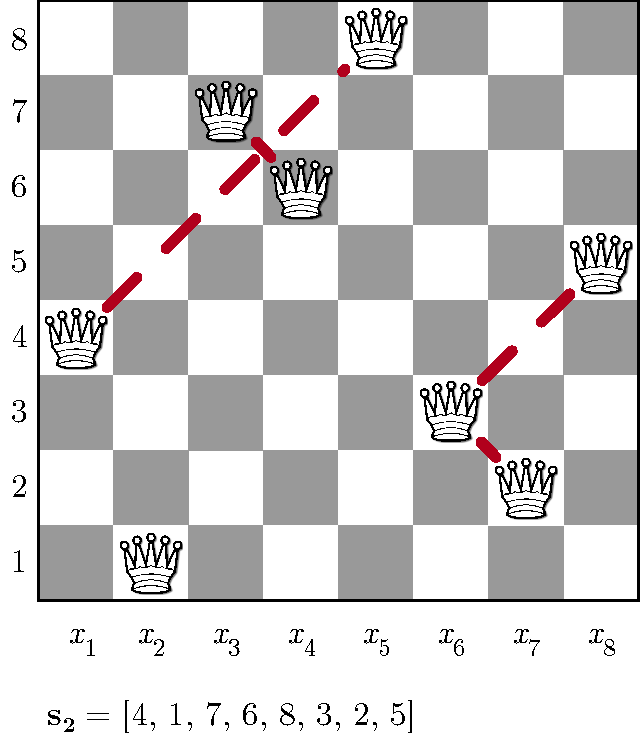
\includegraphics[width=0.4\textwidth]{"Part 2 - Search-Based Optimization/Local Search/n-queens/permutation.pdf"}}
  \end{minipage}
  \leftcaption{A state for the $n$-queens problem in the \textbf{Assignment} search space. \label{fig:nqueens-assignment}}
  \rightcaption{A state for the $n$-queens problem in the \textbf{Permutation} search space (and also in the \textbf{Assignment} one). \label{fig:nqueens-permutation}}
\end{figure}

In the \textbf{Assignment} space, horizontal and diagonal attacks have
to be taken care by the cost function $F$. In the \textbf{Permutation}
space, instead, since the search space is restricted so that two variables
cannot have the same value, also horizontal attacks are prevented by construction. In
this case, the only possible constraint violations come from the
diagonal attacks. It is easy to see that both choices are valid representations in the
sense defined above.

\subsection{Neighborhood Relation}

Given a problem $P$, an instance $I$ and a search space $S$ for it, we
assign to each element $s\in S$ a set $\mathcal{N}(s) \subseteq S$ of
neighboring states of $s$. The set $\mathcal{N}(s)$ is called the
\emph{neighborhood} of $s$ and each member $s'\in \mathcal{N}(s)$ is
called a \emph{neighbor} of $s$.

The set $\mathcal{N}(s)$ does not need to be listed explicitly, but usually
it is implicitly defined by referring to a set of possible
\emph{moves}, which define transitions between states. A move $m$
is defined by a small set of attributes that describe local
modifications of some parts of $s$. We call $s \oplus m$ the state
obtained by the application of move $m$ to state $s$. The ``locality''
of moves is the key ingredient of local search, and it has
also given the name of the whole search paradigm. Nevertheless, from
the definition above there is no implication that there is
``closeness'' in some sense among neighbors, and in fact complex
neighborhood definitions can be used as well.

The only condition that needs to be imposed on the neighborhood relation
$\mathcal{N}$ is that the search space $\mathcal{S}$ is connected
under $\mathcal{N}$. That is, every state $s$ of $\mathcal{S}$ can be
reached from any other state $s'$ by a finite-length sequence of moves
coming from $\mathcal{N}$.

Following the $n$-queens example, we consider two possible
neighborhood relations:

\begin{itemize}\itemsep 2mm
\item \textsf{Change} (\textsf{C}), for \textbf{Assignment} search space:\\
  The move \textsf{C}$\langle q,v\rangle$ assigns value $v$ to variable $x_q$.\\
  \underline{Precondition:} $x_q \neq v$.\\
%  \underline{Example:}   $[3,4,1,7,8,\textbf{4},2,1] \oplus \textsf{C} \langle 6, 1\rangle ~\rightarrow~[3,4,1,7,8,\textbf{1},2,1]$ \\
  
\item \textsf{Swap} (\textsf{S}), for \textbf{Permutation} search space:\\
The move \textsf{S}$\langle q_1,q_2\rangle$ swaps the  values assigned to variables $x_{q_1}$ and $x_{q_2}$.\\
\underline{Precondition:} $q_1\neq q_2$.\\
%\underline{Example:} $[4,\textbf{3},6,5,2,\textbf{1},8,7] \oplus \textsf{S}\langle2, 6\rangle~\rightarrow~[4,\textbf{1},6,5,2,\textbf{3},8,7]$ \\
\end{itemize}

See Figures~\ref{fig:nqueens-change} and~\ref{fig:nqueens-swap} for an example of each move, where the black arrows represent the transitions.

\begin{figure}
  \subfigures 
  \begin{minipage}{\textwidth}
    \leftfigure[t]{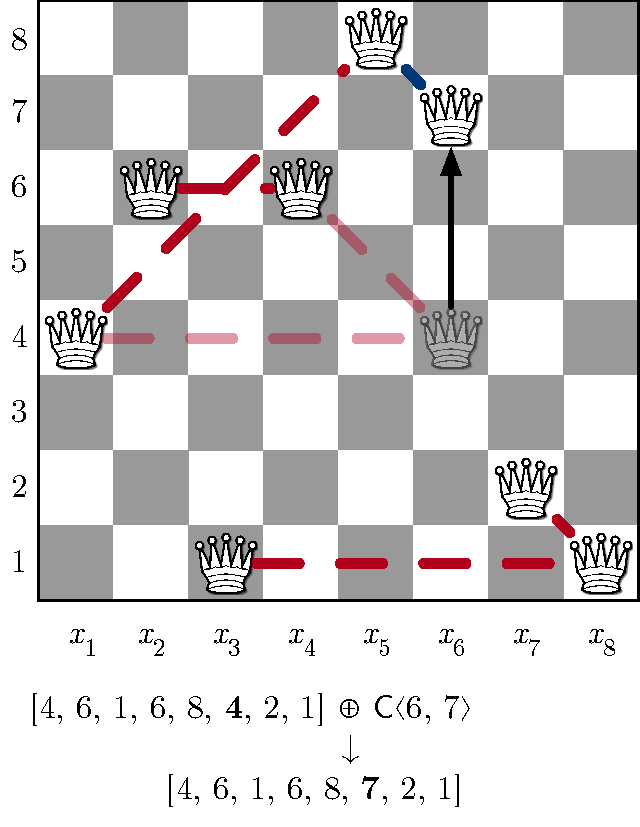
\includegraphics[width=0.4\textwidth]{"Part 2 - Search-Based Optimization/Local Search/n-queens/assignment_change.pdf"}}
    \hspace{\fill}
    \rightfigure[t]{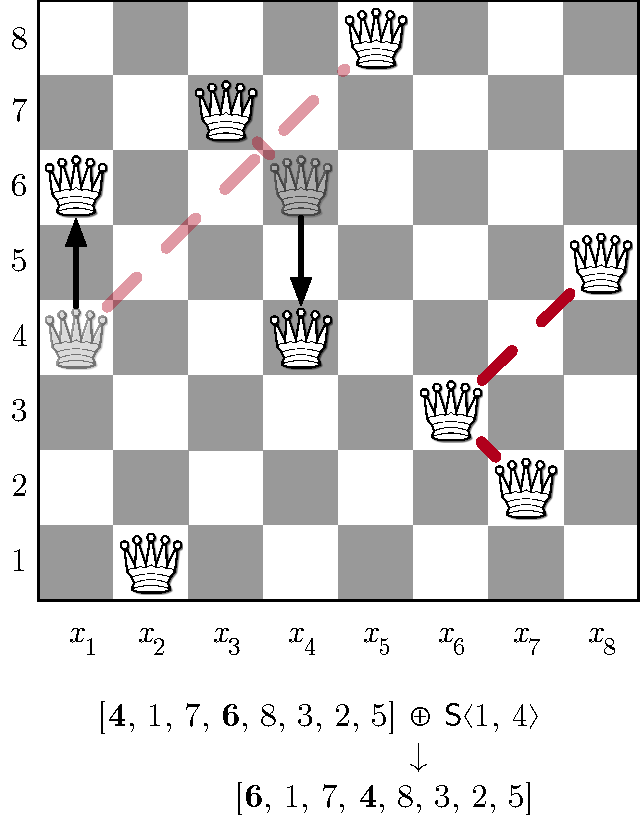
\includegraphics[width=0.4\textwidth]{"Part 2 - Search-Based Optimization/Local Search/n-queens/permutation_swap.pdf"}}
  \end{minipage}
  \leftcaption{An example of \textsf{Change} move. \label{fig:nqueens-change}}
  \rightcaption{An example of \textsf{Swap} move. \label{fig:nqueens-swap}}
\end{figure}


Notice that the \textsf{Change} neighborhood could not be applied to
the \textbf{Permutation} search space, as the moves would lead outside
the search space by duplicating some values. The \textsf{Swap}
neighborhood, instead, can also be applied to the \textbf{Assignment}
search space, but the space would not be connected under this
neighborhood, as the number of repetitions of each value does not
change upon the application of \textsf{Swap} moves, so that certain
states (with different number of repetitions) are never reached.

Nowadays there is a large body of scientific literature that shows the
effectiveness of different neighborhoods on the various problem
domains (e.g., routing and scheduling \cite{IIKM05}).
Nonetheless, the definition of a suitable neighborhood for the
specific novel problem remains a creative activity that the designers
have to undertake using their own intuition and experience. The proof
that the search space is connected under a specific neighborhood is
also a designer's task, which however is relatively easy to do for
most problems. For example, for the $n$-queens problem, for the two
proposed combinations of search space and neighborhood, it is rather
trivial to show that the search space is connected.

One of the key features of the design of the neighborhood relation is
the possibility to compute efficiently the so-called \emph{delta}
function, which is the cost difference between two neighbor states.
For example, for a \textsf{Change} move for the $n$-queens problem,
only the attacks created (resp.\ removed) by the presence in the new
(resp.\ old) position of the specific queen involved in the move needs
to be evaluated. This is easily done in linear time (with respect to
$n$). On the contrary, the full evaluation of the new state obtained
by applying the move would have a quadratic computational cost.

\subsection{Cost Function}

The selection of the move to be performed at each step is based on the
\emph{cost function} $F$ that associates to each element $s\in S$ a
value $F(s)$ that assesses the quality of the solution. For the sake
of simplicity, we assume that the value of $F$ is integer-valued and
non-negative, or in other words, that the co-domain of $F$ is the set
of natural numbers $\mathbb{N}$.

When applied to search problems, the function $F$ normally counts the
number of constraint violations, which is also known as 
\emph{distance to feasibility}. For example, in the $n$-queens
problem, the customary cost function counts the number of attacking
pairs of queens. For the state $s_1 = [4,6,1,6,8,4,2,1]$ 
represented in Figure~\ref{fig:nqueens-assignment},
we have $F(s_1) = 6$, as there are 6 pairs of queens attacking each
other $\{(x_1,x_5), (x_1,x_6), (x_2,x_4), (x_3,x_8),  (x_4,x_6),  (x_7,x_8)\}$ 
connected in the figures with red dotted lines.\footnote{Note that we count also the so-called \emph{X-ray} attacks, i.e. the ones between non consecutive queens in a row (or diagonal) of more than two of them, which by the chess rules would not attack each other.}

In the case of an optimization problem (which, without loss of
generality, is assumed to be a minimization one), $F$ typically merges
together the distance to feasibility and the objective function $f$ of
the problem.  Therefore, the cost function is typically defined as a
weighted sum, with the highest weight assigned to the distance to
feasibility, so as to give preference to feasibility over
optimality. % It seems that optimality is neglected, I would try to rephrase
%
An alternative option is to do not assign weights, but rather consider
the cost function as a pair, and perform the comparison of values in a
hierarchical way, with priority assigned to feasibility.

For some optimization problems the search space can be defined in such
a way that it represents only feasible solutions, and in those cases the cost
function normally coincides with the objective function of the problem.

In some cases, the objective function is complemented by some
auxiliary components which account for ``invisible improvements'' that
incorporate some problem knowledge that is not explicitly considered
in the objective function.  These auxiliary components might be useful
to guide the search toward promising regions of the search space.
As an example of this concept, consider the bin-packing problem for
which the objective is to minimize the number of bins and the selected
neighborhood just moves one object from one bin to another. In this
case, it could be useful to include in the cost function an auxiliary
component that favors states in which bins are filled in an unbalanced
way, rather then a situation in which objects are equally distributed
in the bids. Indeed, such an auxiliary component could create a search
trajectory composed of improving moves leading towards the removal of
one bin. % citation? Sara's phd thesis? Sect 6.3.4

Finally, it is also possible that the cost function is a surrogate of
the real objective function in the case that the latter one is
computationally expensive~\cite{KoCL11}.

\subsection{Initial Solution Selection}

An essential component of any local search procedure is the selection of
the initial solution. Typical choices are a random
generation or the use of a greedy constructive heuristic. It is also possible to use any
other search method to obtain the initial solution.

For example, for the \textbf{Permutation} space for the $n$-queens, the
random state can be obtained by creating the identity permutation
$[1,2,\dots,n]$ and then shuffling it by using the Fischer
and Yates algorithm \cite{FiYa38}.


In order to decide whether to use just a random initial state or spend
some effort to search for a greedy one, we should take into account
different aspects. In fact, on the one hand, a better initial state
would in general require less local search iterations in order to reach
high quality solutions. This saves computational time, which could be used
to perform more steps or more independent runs. On the other hand,
though, it is also possible that the greedy heuristics biases the
search toward some specific regions of the search space, so that it
might become difficult to move away toward different areas.

In some cases, the greedy procedure might be necessary in order to
obtain an initial feasible solution that a random procedure would not
reach. This behavior would allows us to avoid to be forced to include
the distance to feasibility in the cost function by finding a feasible
initial solution, thus simplifying the cost function of the local
search procedure.

% in other cases (eg bin packing) a greedy heuristic finds an initial feasible solution that represents an upper bound, which is then improved by the iterative applying the local search procedure

%For some local search techniques the construction of the initial
%solution is part of the algorithm specification, and thus it is
%required to be done in a certain way.


\subsection{Move Selection and Acceptable Criterion}

At each search step, a single move is selected. The way this selection is
performed characterizes the specific local search strategy, and we
will discuss the different options in the following sections.

However, the selection of a specific move does not inevitably imply that
the move is \emph{accepted} and performed, so that the current state is changed. On
the contrary, the move is normally subject to an acceptance condition,
which is also dependent on the specific technique under consideration.

As a general rule, moves that improve (i.e., decrease) the cost function are
accepted, but also worsening moves (i.e., increasing ones) could be accepted in specific
situations, so as to let the search move away from a \emph{local minimum}.
A local minimum is a state $s$ such that $F(s) \leq F(s')$ for all $s'
\in \mathcal{N}(s)$. When this condition holds also with a strict inequality $<$, 
we call the state a \emph{strict} local minimum. Escaping from local minima is the key issue of all local search techniques.

\subsection{Stop Criterion}\label{sec:stop-criteria}

To end the presentation of the common key elements of local search
we discuss the stop criterion, which determines when the search
is over and the best solution found that far is returned.

Many criteria have been proposed in the literature, starting from the
basic ones, typically based on the expiration of a given amount of time, 
to more complex strategies (see for example \cite[Sect.~3.2]{FrSt19}).
The basic time-expiration strategies can either refer to the wall-clock time or to more
abstract temporal measures, such as the number of iterations. The latter one has the 
advantage of not being machine dependent.

Other options might regard specific qualities of the solution reached
or the so-called \emph{stagnation} detection. That is, when no
improvement is obtained for a given number of iterations, the search is
stopped.  This way, search trials that are exploring promising paths
are let run longer than those that are stuck in regions without good
solutions or where the search is trapped.  It is also possible to
combine different criteria, by stopping the search when the first of a
set of conditions is met.  Similarly to the initial solution
selection, the stop criterion can be part of the specific technique,
therefore we will further discuss it in the following sections.
\vspace{\parskip}

Combining all the key elements presented so far, the pseudocode of a generic local search procedure is shown in
Algorithm~\ref{alg:local-search-pseudocode}.

\begin{algorithm}[ht!]
    %\renewcommand{\baselinestretch}{0.8}
    \caption{LocalSearch} \label{alg:local-search-pseudocode}   
    Parameters: SearchSpace $\mathcal{S}$, Neighborhood $\mathcal{N}$, CostFunction $F$\\   
    Output: $s_{best}$
    \begin{algorithmic}[1]
            \STATE $s \gets InitialState(\mathcal{S})$
            \STATE $s_{best} \gets s$
            \WHILE{\NOT{$StopCriterion$}}
                \STATE $m \gets SelectMove(s,\mathcal{N})$
                \STATE $\Delta F \gets F(s \oplus m) - F(s)$
                \IF{$AcceptMove(m,\Delta F)$}
                    \STATE $s \gets s \oplus m$
            \IF{$F(s) < F(s_{best})$}
                \STATE  $s_{best} \gets s$ \\
            \ENDIF
                \ENDIF
            \ENDWHILE
    \RETURN $s_{best}$
    \end{algorithmic}
\end{algorithm}

The specific definitions of the subprocedures $InitialState$, $StopCriterion$, $SelectMove$, and $AcceptMove$ characterize the specific local search technique.

%%%%%%%%%%%%%%%%%%%%%%%%%%%%%%%%%%%%%%%%%%%%%%%%%%%%%%%%%%%%%%%%%
\section{Basic Local Search Techniques}\label{sec:basics}
%%%%%%%%%%%%%%%%%%%%%%%%%%%%%%%%%%%%%%%%%%%%%%%%%%%%%%%%%%%%%%%%%

The simplest local search techniques are based on some
form of the so-called \emph{Iterative Descent} (also known as
\emph{Iterative Improvement} or \emph{Hill Climbing}).  The idea behind these 
techniques is to select at each step a move that improves the value of the objective
function or reduces the distance to feasibility, never
performing worsening moves.


\subsection{Steepest Descent}

The most well-known form of Iterative Descent is the so-called
\emph{Steepest Descent} (SD) technique. At each iteration, SD selects,
from the whole neighborhood $\mathcal{N}(s)$ of the current state
$s$, the element $s' = s \oplus m$ which has the best value of the
cost function $F$.  The SD procedure accepts the move $m$ only if it
an improving move, i.e., it decreases the value of the cost function. 
Consequently, it naturally stops as soon as it reaches a
local minimum. Therefore, assuming (as customary for combinatorial optimization) that the search space is finite and thus at least one local minimum exists, we don't need to define any other specific stop criterion.

The exhaustive exploration of the neighborhood is obtained by
enumerating the moves in a fixed order.  For example, the
\textsf{Swap} neighborhood for the $5$-queens problem, can be
enumerated in the following lexicographic order: $\{\langle 1,2\rangle, \langle
1,3\rangle, \langle 1,4\rangle, \langle 1,5\rangle, \langle
2,3\rangle, \langle 2,4\rangle, \langle 2,5\rangle, \langle
3,4\rangle, \langle 3,5\rangle, \langle 4,5\rangle\}$.

Notice that if there are two moves that lead to the same state, such as $\langle i,j\rangle$ and $\langle j,i\rangle$ in this case, only one of them should be included in order to prevent wasting time by visiting the same neighbor twice.

The enumeration of the neighborhood raises the issue of tie-breaking
in case of multiple solutions whose value of the cost function is equally good. 
The typical strategy is
to break ties in a uniform random way. That is, if there are $k$
neighbors with the same minimal cost, then each of them might be selected with
probability $1/k$.

\subsection{First-Improving Descent}


The exhaustive neighborhood exploration prescribed by the SD technique might be
rather expensive from the computational point of view. To overcome
this problem, the \emph{First-Improving Descent} (FID) technique accepts a move and moves
to a new neighbor as soon as an improving move is found. FID also
stops when there are no improving moves so that a local minimum is
detected.

In order to avoid the bias toward some specific attributes (e.g., the variables
with low indexes in the above example), the exploration of the
neighborhood should not proceed always in the same fixed order. The
simplest way to avoid such a bias is to start from a random move and
proceed onward in a circular way, by going from the last move to the first one. The procedure stops when the initial
random one is encountered again. For example, the exploration could proceed in the
following order $\{\langle 2,4\rangle,
\langle 2,5\rangle, \langle 3,4\rangle, \langle 3,5\rangle, \langle
4,5\rangle, \langle 1,2\rangle, \langle 1,3\rangle, \langle
1,4\rangle, \langle 1,5\rangle, \langle 2,3\rangle\}$ and stop as soon as an improving move has been found.

\subsection{Random Descent}

Another option to mitigate the computation burden of exhaustive neighborhood exploration 
consists in sampling the neighborhood by drawing random moves. This leads to
the \emph{Random Descent} (RD) technique that draws a (uniform) random move
at each iteration and performs it only if it is improving. 

Care should be taken to ensure that the draw is uniform. Drawing the attributes one at 
the time selecting among available values might bias the search toward moves 
that have a smaller number of possible values for the latest attributes.
For example, for the \textsf{Swap} neighborhood, drawing a random value $i$ between $1$ and 
$n-1$ and then a random value between $i+1$ and $n$, would move the queens with higher indexes move often.


The presence of a local minimum cannot be detected by RD, consequently one of
the stop criteria mentioned in Section~\ref{sec:stop-criteria} should
be used in order to decide when to finish the search.

Notice that the exhaustive exploration of the neighborhood and the random
selection can be seen as two extreme options in the trade-off between
effectiveness and efficiency of the move selection strategy. The
intermediate strategies explore exhaustively only a specific share of the
neighborhood. To this regard, a classical choice is to select randomly
a variable, but exploring all possible alternative values for that
variable and selecting the best one.


\subsection{Non-Ascent Techniques}

All the techniques discussed above can be modified by changing the
acceptance rule so that it accepts also states with equal cost value (the
so-called \emph{sideways} moves). This variant allows the search to move away
from a local minimum, but is still trapped by a strict local minimum.

In this case, we call these methods Non-Ascent techniques, rather than Descent
ones (Steepest, First-Improving, and Random). Non-Ascent
techniques have the ability to navigate through \emph{plateaux},
which are areas of the search space with equal cost, which are often
present in the landscape of many problems.

The navigation through \emph{plateaux} is often useful in reaching states from which the cost can be decreased again. On the other hand, in some cases such navigation might take a long time without producing any improvement.

\section{Discussion}\label{sec:discussion}

In this concluding section of the chapter we discuss some general
issues of local search procedures.

\subsection{Diversification vs.\ Intensification}

The main issue of local search techniques is the way they deal
with the local minima of the cost function. Even if the search
procedure employs some specific mechanism for escaping them (see, e.g., the chapter on Simulated Annealing),
a local minimum still behaves as a sort of \emph{attractor}.
Intuitively, when a trajectory moves away from a local minimum and
steps through a solution ``near'' to it, even though it is not allowed
to go back to the minimum itself, it still tends to move ``forward''
it (i.e., is attracted) instead of moving in an ``opposite'' direction.

For the above reason, the search procedure needs to use some form of
\emph{diversification} strategy that allows the search trajectories
not only to escape a local minimum but to move ``far'' from it thus
avoiding this sort of \emph{chaotic trapping}. 
 
On the other hand, for practical problems the landscape of the
cost function usually has the property that the value is
correlated in neighbors (and near) states.  Therefore, once a good
solution is found, it is reasonable to search in the proximity of it
for a better one. For this reason, when a local minimum is reached the
search should be in some way \emph{intensified} around it.  

In conclusion, the search algorithm should be able to balance two
sometimes conflicting objectives; it should diversify and intensify by
moving outside the attraction area of already visited local minima,
but not too far from it.  


\subsection{Smart Neighborhood Exploration}
%%%%%%%%%%%%%%%%%%%%%%%%%%%%%%%%%%%%%%%%%%%%%%%%%%%%%%%%%%%%%%%%%

Another issue in local search is the computational cost of the
exploration of the neighborhood.  Various ideas have been proposed in
the literature in order to reduce the cost of the exploration, without
penalizing the effectiveness of the search. We mention here just one
idea, known as the \emph{elite candidate list} (see, e.g., \cite[Section 3.2]{GlLa97}).

The mechanism is based on the idea of reusing the evaluations made in the
previous explorations of the neighborhood. The intuition is that if a move $m$
was good in a given solution $s$, very likely it will be still good in the neighbor 
$s' = s \oplus m'$ obtained by performing another move
$m'$.  Based on this intuition, during each neighborhood evaluation, aside selecting the best move, 
we also collect a set of other promising moves (called elite moves). 

In the subsequent iterations, the elite moves previously selected, but
not executed yet, are re-evaluated and possibly executed without
redoing the full exploration. The full exploration, and the
corresponding collection of elite moves, is performed when all
previous elite moves have been executed or discarded.



\subsection{Strategic Oscillation}
\label{sec:strategic-oscillation}
%%%%%%%%%%%%%%%%%%%%%%%%%%%%%%%%%%%%%%%%%%%%%%%%%%%%%%%%%%%%%%%%%

A strategy to overcome the risk of being trapped in a local minimum comes from the manipulation of the cost function.

The cost function of a typical local search procedure is composed by a weighted sum of a
number of components, coming from the distance to feasibility and the objective function
of the problem.  Such weights reflect the relative importance of the
various components of the objective function and the constraints.  

Even though the weights reflect the ``real'' importance of the corresponding
components, to improve effectiveness, their values might be modified during
the search procedure so as to vary the landscape of the cost function. The
temporary modification of the landscape of the cost function, known as \emph{strategic oscillation} 
can help to escape from local minima. 

The idea can be pushed further, by assigning an independent dynamic
weight not to the cost components but to each single constraint.  Such
finer grain weighting could be useful for dealing with problems with
strong asymmetries, i.e., problems in which the number of constraints
involved can be different by a large factor from variable to variable.

An analogous mechanism is based on the idea of adding to the cost
function some additional components which are specifically designed to
escape from local minima. Those extra components are chosen among the
attributes of the elements of the search space in such a way that they
get a high value on the local minimum under
consideration (see, e.g., \cite{VoTA10}).



\subsection{Complex Neighborhoods}

The last topic that we briefly discuss in this introductory chapter on local search regards the neighborhood relation. We know from the literature that for most problems there are various potential neighborhood relations available. Obviously, a state that is a local minimum for one neighborhood might not be a minimum for another neighborhood, so that the alternate use of different ones could help with the key issue of escaping local minima.

Even in cases of one single neighborhood, it is possible to consider chains of moves of length two or more that can be used as alternative relations, which would clearly have different local minima. 

In general, there are different ways to employ more than one neighborhood relation during the search. They range from considering the set-union of all neighborhoods (see, e.g., \cite{BCDS21}), to the interleaving of distinct phases in which the basic neighborhoods are used, to the use of chains of basic moves as the basic neighborhood. 

In all cases, the resulting neighborhood relation would be rather large and the exhaustive exploration problematic from the efficiency point of view. The discussion on how to explore a large neighborhood is complex and it is outside the scope of this chapter (see \cite{AEOP02}). 

\section{Exercises}

\begin{exercise}
Consider the classical \emph{graph coloring} problem, in which a given indirected graph has to be colored with a fixed number of colors avoiding that two adjacent nodes have the same color. Define a valid search space, a suitable neighborhood relation, and the cost function for this problem. 
\end{exercise}

\begin{exercise}\label{exe:flow-shop}
Consider the classical \emph{permutation flow-shop} problem, in which the order of a set of \emph{jobs} and the start and end times of their processing on a predetermined sequence of machines has to be decided. The objective is to minimize the \emph{makespan}, that is the latest completion time of a job on the last machine. Define a valid search space, one or more suitable neighborhood relations, and the cost function for this problem. 
\end{exercise}

\begin{exercise}
Consider the problem of Exercise~\ref{exe:flow-shop}, with in addition the presence of \emph{strict} due dates for the jobs, that is each job must be completely processed within its due date. How do you modify the cost function? Conversely, if the due dates are soft and the problem requires to minimize the total \emph{tardiness}, i.e., the summation of the lateness of each job, how is the cost function defined in this case?
\end{exercise}


\bibliographystyle{unsrt}
\bibliography{local_search}

\title{Simulated Annealing}
\label{chp:simulated-annealing}
\author{Alberto Franzin, Thomas St\"utzle}
\institute{Universit\'e Libre de Bruxelles}
\maketitle

\urldef\supplementurlsa\url{https://github.com/ieee-cis/IEEE-CIS-Open-Access-Book-Volume-1/tree/main/Part%202%20-%20Search-Based%20Optimization/Simulated%20Annealing/SupplementaryMaterial}

\newcommand{\initialtemperature}{\textsc{Initial Temperature}\xspace}
\newcommand{\stoppingcriterion}{\textsc{Stopping Criterion}\xspace}
\newcommand{\explorationcriterion}{\textsc{Neighbourhood Exploration}\xspace}
\newcommand{\acceptancecriterion}{\textsc{Acceptance Criterion}\xspace}
\newcommand{\temperaturelength}{\textsc{Temperature Length}\xspace}
\newcommand{\coolingscheme}{\textsc{Cooling Scheme}\xspace}
\newcommand{\temperaturerestart}{\textsc{Temperature Restart}\xspace}
\newcommand{\initialsolution}{\textsc{Initial Solution}\xspace}
\newcommand{\neighbourhood}{\textsc{Neighbourhood}\xspace}
\newcommand{\brsa}{\texttt{BR1}\xspace}
\newcommand{\qsa}{\texttt{Q8-7}\xspace}

\label{sec:introduction}

The origins of simulated annealing lie in the work of Metropolis 
\textit{et al.} in statistical physics \cite{MetRosRosTel53}, who proposed an algorithm to simulate the displacement of particles in
a solid body. A random displacement is effectively performed (``accepted'')
if it lowers the total energy of the system, while it is performed with 
probability $\exp{(-\Delta E / k_BT)}$ if the energy variation $\Delta E$ is
positive. In the Metropolis formula, $k_B$ is the Boltzmann constant and $T$
is the temperature at which the displacement is evaluated.
For a temperature value $T$, the higher $\Delta E$, the lower the chance
the displacement effectively happens. Likewise, if the given $\Delta E$ is held constant but positive,
the higher the temperature, the higher the probability of the displacement.

In one of the first
instances of algorithmic development inspired by natural phenomena, 
Kirkpatrick, Gelatt and Vecchi \cite{Kirkpatrick83},
and independently \v{C}erny \cite{Cer85}, thought to
view a combinatorial optimization problem as a solid, whose states are the
feasible solutions of the problem. The objective function value of
a particular solution is related to the level of energy of the system in
a particular configuration. The system is first heated
and then cooled little by little until it ``freezes''. 
Out of the metaphor, the algorithm starts from an initial solution
and iteratively evaluates candidate ones.
The temperature used to evaluate an exchange starts at a high value,
and is progressively lowered following a geometric trend. For temperature
values low enough, the probability of accepting worsening moves becomes
effectively zero, and the algorithm behaves like an iterative improvement.


The function originally proposed to determine the acceptance
or the rejection of a move is the so-called \textit{Metropolis criterion} \cite{MetRosRosTel53},
where a solution of equal or better quality is accepted always. If, however, the new solution $\mathbf{x^\prime}$ is worse than 
the current solution $\mathbf{x}$, it is accepted with a probability $\exp{(-(f(\mathbf{x^\prime}) - f(\mathbf{x}))/T)}$ for 
minimization or with a probability $\exp{(f(\mathbf{x^\prime}) - f(\mathbf{x})/T)}$ for maximization problems, where $f(\cdot)$ is the objective function. 
Here, we always will assume minimization problems; it is straightforward 
to adapt the algorithm for a maximization problem.
The probability of accepting worsening moves depends 
on the relative worsening in terms of
solution quality from the incumbent one and on the scalar parameter $T$, called \textit{temperature}.
For a proposed worsening move, high values of the temperature parameter provide a higher chance of 
accepting it than lower values. High temperature values therefore promote a stronger exploration behaviour,
while low values are associated to a strong exploitation.
Simulated annealing can thus be considered as a local search with 
a diversification mechanism governed by the temperature parameter.

The choice of the value for the temperature parameter is crucial in obtaining good results. 
The original formulation, the conventions and the folklore deriving
from the annealing metaphor, but
also the theoretical works on simulated annealing, make use of a sequence of values.
In general, the temperature value is set at a ``high'' initial value,
and progressively decreased to a final ``low'' value, to make
the algorithm transition from a highly exploration behaviour to a converging,
exploitative one. Optionally, the temperature value is raised again or restored
to its initial value, to promote a cycle of diversification and intensification
phases.

Immediately after its introduction, simulated annealing attracted the attention of 
several researchers, thanks to its simple formulation and the quality
of the results obtained in several works. 
It became therefore one of the most popular algorithms for combinatorial
optimization problems, and it has been used in thousands of works.
Along with its use, researchers became interested in modeling its behaviour from
a theoretical perspective. A series of works, mostly in the 80s' and early 90s',
focused on conditions for the cooling scheme to obtain the optimal solution for a
given problem and instance, mostly under unrealistic conditions such as an
infinite number of evaluations \cite{GemGem1984,LundyMees1986,Hajek1988,RomSan1991}. 
Yet, by simply enumerating the
search space one could guarantee to find the optimal solution even in
finite time but, in the end, very large time which is usually infeasible.  
Thus, a more important question would refer to the
convergence speed of simulated annealing, that is, how quickly good solutions are found; yet, results addressing this
question are rare. Also, practical annealing schedules decrease the
temperature much faster than what is implied by the theoretical results and
therefore the convergence proofs do not apply in this case. 

In this chapter we summarize research on simulated annealing and its behaviour.
We show how implementing a simulated annealing algorithm can be seen as a configuration task,
and makes use of efficient artificial intelligence tools to automatically generate high-performing
algorithms for different scenarios. We then explore quickly the results and the algorithms we 
obtain and then conclude the chapter.



\section{A simulated annealing algorithm}

\subsection{A basic simulated annealing algorithm}


Implementing a basic simulated annealing algorithm is quite fast. First, one needs a starting 
solution, which can be a uniformly random solution in the simplest case, or one computed using a simple heuristic
like a constructive one. 
Second, one needs a neighbourhood, which is an essential ingredient. 
Sometimes the neighbourhood can be more complicated as 
for some problems one needs to have various neighbourhoods and decide how to schedule them. Then one has to choose a 
simulated annealing acceptance criterion. As the simplest one,
use the Metropolis criterion, which we have detailed in the introduction of this chapter
 \cite{MetRosRosTel53,JohAraMcGSch1989,JohAraMcGSch1991}. As a reminder, an 
improving or equal move is always accepted and a worsening one is accepted with a probability 
$\exp{(-(f(\mathbf{x^\prime}) - f(\mathbf{x}))/T)}$. The rest is embedding the annealing criterion in an 
\textit{annealing schedule}, which is also called \textit{cooling schedule}. 
It is defined by an initial temperature $T_0$, a scheme saying how the new temperature is
obtained from the previous one, the number of search steps to be performed at
each temperature, and a termination condition. A common choice is in simulated annealing to use
a geometric cooling, which is that  $T_{i+1} = \alpha T_i$, where $\alpha$ is a parameter 
with $0 < \alpha < 1$. This operation, called annealing step, is usually done 
after a number of search steps (that is, candidate solution evaluations) performed at 
the same temperature, often for a number of evaluations that is a multiple of the neighbourhood size. 
Finally the termination criterion is often based on the acceptance ratio, that is, 
the ratio of proposed steps versus the accepted steps. 

\subsection{A component-based overview of simulated annealing}
\label{sec:sacomponents}

To use a full-fledged simulated annealing one has to set still 
the control parameters, such as the initial temperature value,
the temperature update factor, or the number of moves to be evaluated at the same temperature.
We have now a somewhat reasonable algorithm and
in the meantime, with the thousands of papers, much more involved 
simulated annealing algorithms have been proposed. So in 
\cite{FraStu2019:cor}, we identified a total 
of seven components, whose function and connection
define what a simulated annealing is, and how it works. Two other components 
are necessary to elaborate information for the specific problem considered,
and are not unique to simulated annealing. Problem-specific components can be considered as 
inputs to simulated annealing.
The outline is given in Algorithm \ref{algo:simannealing}, and the components
are subsequently described.

\begin{algorithm}[ht!]
	  \caption{Component-based formulation of SA. The components we
      have identified for our analysis are written in \textsc{Smallcaps}.}
     \label{algo:simannealing}
    
    Parameters: a problem instance $\mathcal{I}$, a \neighbourhood $\mathcal{N}$ for the solutions, an \initialsolution $\mathbf{x}_0$, control parameters
    
    Output: the best solution $\mathbf{x^*}$ found during the search.
    
	\begin{algorithmic}[1] 
		\STATE{$\textrm{best solution } \mathbf{x^*} := \textrm{incumbent solution } \mathbf{\hat{x}} := \mathbf{x}_0$\;}
		\STATE{$i := 0$\;}
        \STATE{Initialize temperature $T_0$ according to \initialtemperature\;}
		\WHILE{\stoppingcriterion is not met}
		\STATE{choose a solution $\mathbf{x}_{i+1}$ in the \neighbourhood of $\mathbf{\hat{x}}$ according to \explorationcriterion criterion\;}
		\IF{$\mathbf{x}_{i+1}$ meets \acceptancecriterion}
		\STATE{$\mathbf{\hat{x}} := \mathbf{x}_{i+1}$\;}
		\IF{$\mathbf{\hat{x}}$ improves over $\mathbf{x^*}$}
		\STATE{$\mathbf{x^*} := \mathbf{\hat{x}}$\;}
		\ENDIF
		\ENDIF
		\IF{\temperaturelength is met}
		\STATE{update temperature according to \coolingscheme\;}
		\STATE{reset temperature according to \temperaturerestart scheme\;}
		\ENDIF
		\STATE{$i := i + 1$\;}
		\ENDWHILE
        \STATE{return $\mathbf{x^*}$\;}
	\end{algorithmic}
	
\end{algorithm}

{\initialtemperature.}
The initial value of the temperature parameter, and, usually, the
maximum value the temperature will take. It also defines the maximum amount of 
diversification, that is, how likely the algorithm is to accept worsening moves,
and it is therefore best computed starting from instance characteristics. 
For example, the initial temperature can be set proportionally to the initial solution value, 
or computed according to some search space statistics such as the maximum gap 
or the average gap between consecutive moves computed during a preliminary random walk.

{\initialsolution (problem-specific).}
Simulated annealing starts from an initial solution that has to be provided 
by a problem-specific component, for example, using a
constructive heuristic, another local search, or even a
random solution. Anyway, if one starts from a problem-specific, 
good candidate solution one should use a low temperature start, since 
otherwise the initial solutions gets destroyed. 

{\neighbourhood (problem-specific).}
The neighbourhood function generates the solutions that are at
distance of one move from the incumbent one. This is also the
component that deals with constraints when necessary, repairing 
infeasible solutions or ensuring that the candidate solutions
generated are feasible. In the simplified environment this is one 
neighbourhood, but it may be that for other problems various 
neighbourhoods are important. 

{\explorationcriterion.}
This component is devoted to selecting one candidate solution to evaluate for acceptance, in the neighbourhood
of the incumbent one. The traditional simulated annealing uses the random selection of a neighbour solution, but alternative
schemes are possible, such as a sequential evaluation following an enumeration
of the solution in the neighbourhood, or even mini-local searches \cite{COnnolly1990,IshMisTan1995}.

%\paragraph
{\acceptancecriterion.} 
The function that determines whether the solution selected by the 
\explorationcriterion should be accepted and replace the incumbent.
The traditional and most popular criterion is the Metropolis condition described at the beginning of this chapter,
but several other criteria have been proposed.
Notably, the Threshold Acceptance is a deterministic variant of simulated annealing 
that always accepts candidate moves that worsen the solution quality of an amount bounded by the temperature value
\cite{DueSch90,MosFon1990}. The Late Acceptance Hill Climbing can also 
be considered as an acceptance criterion that can be fit in the simulated annealing 
structure \cite{BurByk2017}. This latter scheme maintains a history of accepted moves,
and always accepts a candidate solution that is improving over either
the incumbent one, or the incumbent solution of $\kappa$ iterations before.

%\paragraph
{\coolingscheme.}
The function that controls the decrease of the temperature parameter.
The original simulated annealing papers use a geometric criterion, that decreases the temperature
value by a multiplicative factor $\alpha \in (0,1)$, i.e. $T_{i+1}=\alpha T_i$, with $\alpha$ constant throughout
the whole search \cite{Kirkpatrick83,Cer85}. In accordance with the annealing metaphor and the idea of
transitioning from exploration to exploitation, cooling schemes generally yield
monotonically decreasing sequences of temperature values. Some authors have,
however, deviated from the annealing behaviour and proposed schemes that
always keep the same temperature value, or have the temperature value
``fluctuate'', allowing for phases of both controlled increase and decrease
of the temperature parameter \cite{HuKahTsa95}. 
This fluctuation is intended to exhibit a behaviour similar to a fixed temperature value,
while at the same time promoting alternating phases of limited exploration and exploitation,
thus bridging the two opposite SA behaviours.

%\paragraph
{\temperaturelength.}
This component controls the amount of candidate solutions that will be
evaluated using the same temperature value; in other words, it determines when
the \coolingscheme should be used.
The simplest options are constant values, either absolute or proportional to 
some problem characteristic such as instance or neighbourhood size
\cite{HusStu2014cor,JajMinHarPro1992}. However, 
adaptive schemes that make the decision on when to update the temperature 
based on the outcome of the search (for example, a certain amount of accepted moves \cite{Abramson1991})
can provide a more fine-grained control of the exploration/exploitation
trade-off.

%\paragraph
{\temperaturerestart.}
This component determines if and when the temperature value
should be reset to its original value, or set to another higher value (reheat).
Its purpose is to promote a new phase of exploration once the temperature has 
decreased enough to void its diversification potential.
As for the \temperaturelength there are many possibilities, both constant and
adaptive \cite{Kirkpatrick1984,AbrAmoDan1999}.

{\stoppingcriterion.}
The last algorithmic component determines when the search terminates.
This can be set according to fixed conditions such as a given runtime
or amount of moves evaluated, or adaptive conditions such as a too low
acceptance rate \cite{JohAraMcGSch1989,JohAraMcGSch1991}.


\subsection{Composing efficient simulated annealing algorithms}
To implement a new or existing simulated annealing, the developer needs
to face several choices. First of all, 
it is necessary to define the choices
that are related to the specific problem considered, that is, an initial
solution from where to start the search, and the neighbourhood function
used to generate new candidate solutions.
Then the search components, that determine how to select a new candidate
solution, whether to accept it, and how to update the control parameters
have to be implemented.

Since the structure of SA is fixed, designing a simulated annealing algorithm
means to choose which components and which numerical parameters
to use. 
A good starting point to determine which choices to make is the existing body of literature.
Even when limiting ourselves to the algorithm-specific components,
we can find plenty of options for each one of them. 

\begin{table}[tb]
    \centering
    \caption{List of options we implemented for the algorithmic components of simulated annealing. 
    Several of these components include additional numerical parameters. 
    For a more formal description of each component and their implementation we refer to \cite{FraStu2019:cor}.}
    \begin{tabular}{l p{8.2cm}}
       \initialtemperature  & Fixed value; proportional to initial solution value; proportional to maximum gap in random walk; proportional to average gap in random walk; Connolly initial temperature scheme;  Misevicius initial temperature scheme; simplified Misevicius initial temperature scheme. \\
    \explorationcriterion  & Random; sequential; Ishibuchi-Misaki-Tanaka 1; Ishibuchi-Misaki-Tanaka 2. \\
    \acceptancecriterion & Metropolis; bounded Metropolis; precomputed Metropolis; Generalized simulated annealing; geometric acceptance; Threshold acceptance; Great Deluge; Record-to-Record; Late Acceptance Hill Climbing; Hill Climbing.\\
    \coolingscheme & Geometric 1; geometric 2; Lundy-Mees 1; Lundy-Mees 2;
    Q8-7; quadratic; arithmetic; no cooling; temperature band. \\
    \temperaturelength & Fixed; \# moves proportional to problem size; proportional to neighbourhood size; \# of accepted moves; bounded (\# accepted moves, max \# moves); arithmetic increase; geometric increase; logarithmic increase; exponential increase.\\
    \temperaturerestart & Never; Restart or reheat based on: \# moves; minimum temperature value; \% of initial temperature value; global acceptance rate; acceptance rate in the last moves; no recently accepted moves. \\
    \stoppingcriterion & runtime; \# moves; minimum temperature; \# cooling steps; \# temperature restarts; \# moves with no accepted solution; global acceptance rate; most recent acceptance rate; no new recent best solution.\\
    \end{tabular}
    \label{tab:options}
\end{table}

In \cite{FraPerStu2018ol} we collected a total of 66 different options for all the
components, reported in Table \ref{tab:options}, which are enough 
to assemble millions of valid simulated annealing
algorithms. Many of those components have their own set
of numerical parameters to choose \cite{HutHooLey2011lion,LopDubPerStuBir2016irace}. 

The traditional, manual implementation of an algorithm is effectively
an exploration of the space of possible valid algorithms. Finding the one
that performs the best over the entire application space (i.e. the whole test set)
is clearly a daunting task.
Developers therefore often revert on results from the
literature and on established practices and conventions. The first 
reasonable algorithm, either assembled or found in the literature,
is then fine-tuned on a limited set of instances.

Aside from being tedious, this process has several drawbacks. 
First, the combination of components and parameters raises a
complex interaction that is often unexpected
to the user. The developer is then forced to evaluate a restricted set of
options on a limited set of instances, thus prioritizing the
algorithmic solutions already explored in past applications and
in the literature. The bias that follows from this process
likely results in sub-optimal algorithms, whose behaviour and
results are unexplained.

In this chapter we demonstrate how the use of powerful algorithm
engineering tools is beneficial in automatically designing simulated annealing
algorithms that can outperform manually designed ones.
We follow the Programming by Optimization philosophy
that envisages increasing levels of automation of the development process
\cite{Hoos:PbO}. 
The implementation of an algorithms moves away
from a purely manual task, to one that relies on automatic tools
to improve existing algorithms, towards an automatic design of new algorithms.

This task can be framed as a machine learning one
\cite{Birattari09tuning}. In a nutshell, our goal is to find 
the parameter configuration that obtains the best results on a \textit{test set} 
of instances, that ideally represent a realistic practical application. 
In absence of an explicitely structured knowledge on the relationship
between configurations and instance characteristics in terms of results, 
we employ a \textit{training set} of instances, different from the test set 
but belonging to the same distribution. On this training set we 
select the configuration with the best results overall.
For more detailed instructions we refer to the existing literature, 
e.g. \cite{Hoos:PbO,MasLopDubStu2014cor,StuLop2019hb,PagStu2019:ejor} in general,
and \cite{FraStu2019:cor} for SA specifically.



\section{Experiments}
\label{sec:exp}


\subsection{Materials and methods}\label{sec:material}
We consider the Quadratic Assignment Problem (QAP), one of the classic NP-hard
problems where we want to find the assignment of $n$ facilities to $n$ locations
with the minimal cost \cite{KooBec57}. A QAP instance is defined by two
matrices, one with the distances $D_{k,l}$ between two locations $k$ and $l$, and
one with the flows $F_{i,j}$ between two facilities $i$ and $j$.
We represent a solution as a permutation $\pi$, whose
elements $\pi(i)$ contain the location of facility $i$. The objective function is
\begin{equation}
  \min\sum_{i=1}^n\sum_{j=1}^n F_{ij} D_{{\pi(i)}{\pi(j)}}.
\end{equation}

We use two groups of different QAP instances. In the first one the distance matrices 
define a structure in the landscape, and we refer to it as the class of \textit{structured} instances. 
In the second one, instead, the matrices are generated
uniformly at random, and we call this the \textit{random} instances class.
Each class
contains $100$ instances of sizes $60$, $80$ and $100$, equally partitioned into
a training set and a test set.
The training set is used to automatically configure 
and design the algorithms using irace, and the test set is used to 
evaluate the configurations obtained, whose results are reported
in the rest of this section.
Every simulated annealing execution runs for ten seconds.
We use the EMILI framework,
where we implemented 66 components and the relative numerical parameters,
for a total of 100 configurable parameters \cite{PagStu2019:ejor}.
We use a budget of $2000$ experiments to configure the numerical parameters
of two existing simulated annealing algorithms, and we automatically design simulated annealing algorithms
using $10$K, $20$K, $40$K and $80$K experiments, where one experiment is a SA run.
The experiments are done on a machine with two Intel Xeon E5-2680v3 CPUs 
at 2.5GHz with 16MB cache, with 2.4GB of RAM available for each experiment.

The algorithm configurator irace implements the iterated racing algorithm 
in an easy-to-use \texttt{R} package
\cite{LopDubPerStuBir2016irace,BirStuPaqVar02:gecco,MarMoo1997air}. 
The basic idea is to spend computational budget only on configurations
that are worth evaluating, rather than waste it on poor ones.
To configure an algorithm it requires only the definition of the parameters,
a training set of instances, and a script that executes the algorithm with 
a list of command-line parameters (provided by irace as input to the script) 
and returns a measure of the quality of the configuration observed on the instance. 
Such metric defines the configuration task as an optimization problem, and commonly 
used ones include the solution quality found by heuristic algorithms, 
or the runtime needed to find the optimal solution.
irace starts from a set of random configurations, and begins to evaluate all of them 
on the training instances, sequentially. The configurations are ranked for each instance, 
based on the results reported. After a few instances, irace begins to discard the configurations 
that perform statistically worse than the best ones, and proceeds to evaluate only the surviving ones. 
This process of configuration evaluation and statistical test, called \textit{race}, 
is iterated until either the budget for evaluations is exhausted, or a minimum number 
of surviving configuration remains. At this point, new configurations are sampled, 
with parameter values around the surviving configurations, and a new race takes place. 
Race after race, the new configurations get sampled increasingly closer to the last best ones.
When the total evaluation budget is terminated, irace returns to the user the best configurations found.

EMILI is a \texttt{C++} algorithmic framework for the development of modular 
stochastic local search algorithms \cite{PagStu2019:ejor}.
Algorithms are instantiated at runtime by selecting the desired combination of 
command-line parameters, that determine which components and numerical parameters 
are selected, and how they are combined.
The modular structure of EMILI makes it possible to design algorithms
bottom-up, so, in principle, of any shape.
However, its flexibility can of course be exploited to design algorithms 
of a given structure, as we do in this chapter by requiring the components 
to be placed in their proper place in the template of simulated annealing
in Algorithm \ref{algo:simannealing}.

\subsection{Simulated annealing algorithms for the QAP}
\label{sec:expsqap}

We start by reproducing two of the many simulated annealing algorithms
proposed for QAP. These algorithms are called \brsa and \qsa
\cite{BurRen1984,COnnolly1990}. 
The only common algorithmic component between the two algorithms is the Metropolis
acceptance criterion. 
\brsa  starts from an initial temperature computed as the maximum gap observed between
consecutive solutions in a random walk \cite{BurRen1984}.
It uses the random exploration of the neighbourhood to select a move to evaluate.
The temperature is updated with a geometric cooling scheme with coefficient $0.5$
every $2 \times n$ proposed moves, where $n$ is the problem size, and restarted 
to its original value after $|N(\mathbf{x})|$ moves, that is, the size of the neighbourhood.
\brsa therefore performs only a few but substantial temperature updates.
In its original formulation, \brsa terminates its search after $10$ temperature
restarts.

The \qsa algorithm from \cite{COnnolly1990} 
uses a custom mechanism to define the initial temperature, relating it to
the final one.
This algorithm uses a sequential exploration of the neighbourhood to select candidate moves,
imposing an order on the solutions in the neighbourhood and following it.
One particular characteristic of this algorithm is the \texttt{Q8-7} cooling scheme,
an adaptation of the Lundy-Mees cooling scheme \cite{LundyMees1986}. After the cooling phase, once $m$
consecutive moves have been rejected, this scheme restores the temperature to the value at which
the current best solution was found, forces the acceptance of the current 
proposed move, and stops the temperature update, keeping the same value until the end of the search.
The $m$ parameter is set proportionally
to the total number of moves evaluated by the algorithm.
During the initial cooling phase of the \texttt{Q8-7}, the temperature is lowered 
after every move evaluated, and there is no temperature restart.
The algorithm as reimplemented from the original paper terminates after
$50 \times |N(\mathbf{x})|$ moves.

Both algorithms start from a randomly generated permutation, and use the
$2$-exchange neighbourhood
\begin{equation}
  \mathcal{N}(\pi) = \{\pi'\:|\: \pi'(j) = \pi(h) \wedge
  \pi'(h) = \pi(j) \wedge \forall l \notin \{j,h\}\: :\pi'(l)
  = \pi(l) \} 
\end{equation}
that swaps two elements in positions $i$ and $j$ in a solution $\pi$. In total, \brsa has five tunable numerical parameters, 
while \qsa has six; as we will not tune the termination condition, this number reduces 
to respectively four and five. The pseudocode for \brsa and \qsa is reported, respectively, in Algorithms 
\ref{algo:brsa} and \ref{algo:qsa}.

\begin{algorithm}[ht!]

	  \caption{Component-based formulation of \brsa with its original parameters. 
	  The components are highlighted in \textit{italic}. The 
      tuned numerical parameters we obtained are: 
      $\theta^\prime = (k = 8.979, \beta = 51, \alpha = 0.9163, \gamma = 83)$ 
      for the structured instances and $\theta^\prime = (k = 6.3173, 
      \beta = 94, \alpha = 0.9206, \gamma = 79)$ for the random instances, 
      and the termination is replaced with a time-based one ($10$ seconds).}
     \label{algo:brsa}
    
    Parameters: a problem instance $\mathcal{I}$, the \textit{$2$-exchange neighbourhood}, 
    \textit{a random permutation $\mathbf{x}_0$}, control parameters 
    $\theta = (k = 1, t = 10, \beta = 2, \alpha = 0.5, \gamma = 1)$
    
    Output: the best solution $\mathbf{x^*}$ found during the search.
    
	\begin{algorithmic}[1] 
		\STATE{$\textrm{best solution } \mathbf{x^*} := \textrm{incumbent solution } \mathbf{\hat{x}} := \mathbf{x}_0$\;}
		\STATE{$i := 0$\;}
        \STATE{Initialize temperature $T_0$ as \textit{the max gap between consecutive solutions in a random walk of length $l=10^4$, with a scaling factor $k$} \;}
		\WHILE{\textit{less than $t$ temperature restarts have happened}}
		\STATE{choose a solution $\mathbf{x}_{i+1}$ in the \textit{$2$-exchange neighbourhood} of $ \mathbf{\hat{x}}$ \textit{at random}\;}
		\IF{$ \mathbf{x}_{i+1}$ meets \textit{Metropolis criterion}}
		\STATE{$ \mathbf{\hat{x}} := \mathbf{x}_{i+1}$\;}
		\IF{$ \mathbf{\hat{x}}$ improves over $\mathbf{x^*}$}
		\STATE{$\mathbf{x^*} :=  \mathbf{\hat{x}}$\;}
		\ENDIF
		\ENDIF
		\IF{$\beta$ \textit{times the instance size number of moves have been evaluated}}
		\STATE{update temperature according to \textit{geometric cooling with factor} $\alpha$\;}
		\STATE{reset temperature \textit{to initial value $\gamma$ times the neighbourhood size}\;}
		\ENDIF
		\STATE{$i := i + 1$\;}
		\ENDWHILE
        \STATE{return $\mathbf{x^*}$\;}
	\end{algorithmic}
	
\end{algorithm}
\begin{algorithm}[ht!]
	  \caption{Component-based formulation of \qsa with its original parameters. 
	  The components are highlighted in \textit{italic}. The 
      tuned numerical parameters we obtained are: $\theta^\prime = (k = 6.7411, 
      \alpha = 0.9114, \beta = 0.2183, m = 600676, j = 97)$ for the structured instances and 
      $\theta^\prime = (k = 5.5683, \alpha = 0.8597, \beta = 0.04, m = 234615, j = 76)$ 
      for the random instances, and the termination is replaced with a time-based one ($10$ seconds).}
     \label{algo:qsa}
    
    Parameters: a problem instance $\mathcal{I}$, the \textit{$2$-exchange neighbourhood}, 
    \textit{a random permutation $\mathbf{x}_0$}, control parameters 
    $\theta = (k = 1, t = 10, \alpha = 1, \beta = 1, m = |N(s)|, j = 1)$
    
    Output: the best solution $\mathbf{x^*}$ found during the search.
    
	\begin{algorithmic}[1] 
		\STATE{$\textrm{best solution } \mathbf{x^*} := \textrm{incumbent solution } \mathbf{\hat{x}} := \mathbf{x}_0$\;}
		\STATE{$i := 0$\;}
        \STATE{Initialize temperature $T_0$ according to \textit{custom formula \cite{COnnolly1990}, with scaling factor $k$} \;}
		\WHILE{\textit{less than $t\times |N(\mathbf{x})|$ moves} have been evaluated}
		\STATE{choose a solution $\mathbf{x}_{i+1}$ in the \textit{$2$-exchange neighbourhood} of $\mathbf{\hat{x}}$ using a \textit{sequential neighbourhood exploration}\;}
		\IF{$ \mathbf{x}_{i+1}$ meets \textit{Metropolis criterion}}
		\STATE{$ \mathbf{\hat{x}} := \mathbf{x}_{i+1}$\;}
		\IF{$ \mathbf{\hat{x}}$ improves over $\mathbf{x^*}$}
		\STATE{$\mathbf{x^*} :=  \mathbf{\hat{x}}$\;}
		\ENDIF
		\ENDIF
		\IF{\textit{$j$ moves have been evaluated}}
		\STATE{update temperature according to \textit{Q8-7 cooling scheme with parameters $\alpha$, $\beta$, $m$}\;}
		\STATE{\textit{never} reset temperature\;}
		\ENDIF
		\STATE{$i := i + 1$\;}
		\ENDWHILE
        \STATE{return $\mathbf{x^*}$\;}
	\end{algorithmic}
	
\end{algorithm}

\subsubsection{Reinstantiating and improving existing algorithms} 
We start with three types of experiments.
In the first one we run the algorithms using their original parameter settings, including the
termination (thus resulting in different running times);
in the second one we take the original parameters but force each algorithm to run for 10 seconds; and a third one where we tune the parameters with irace, forcing an algorithmic runtime of 10 seconds. 
The results are reported in Figure \ref{fig:resqap1}.

\begin{figure}[tb]
  \begin{center}
    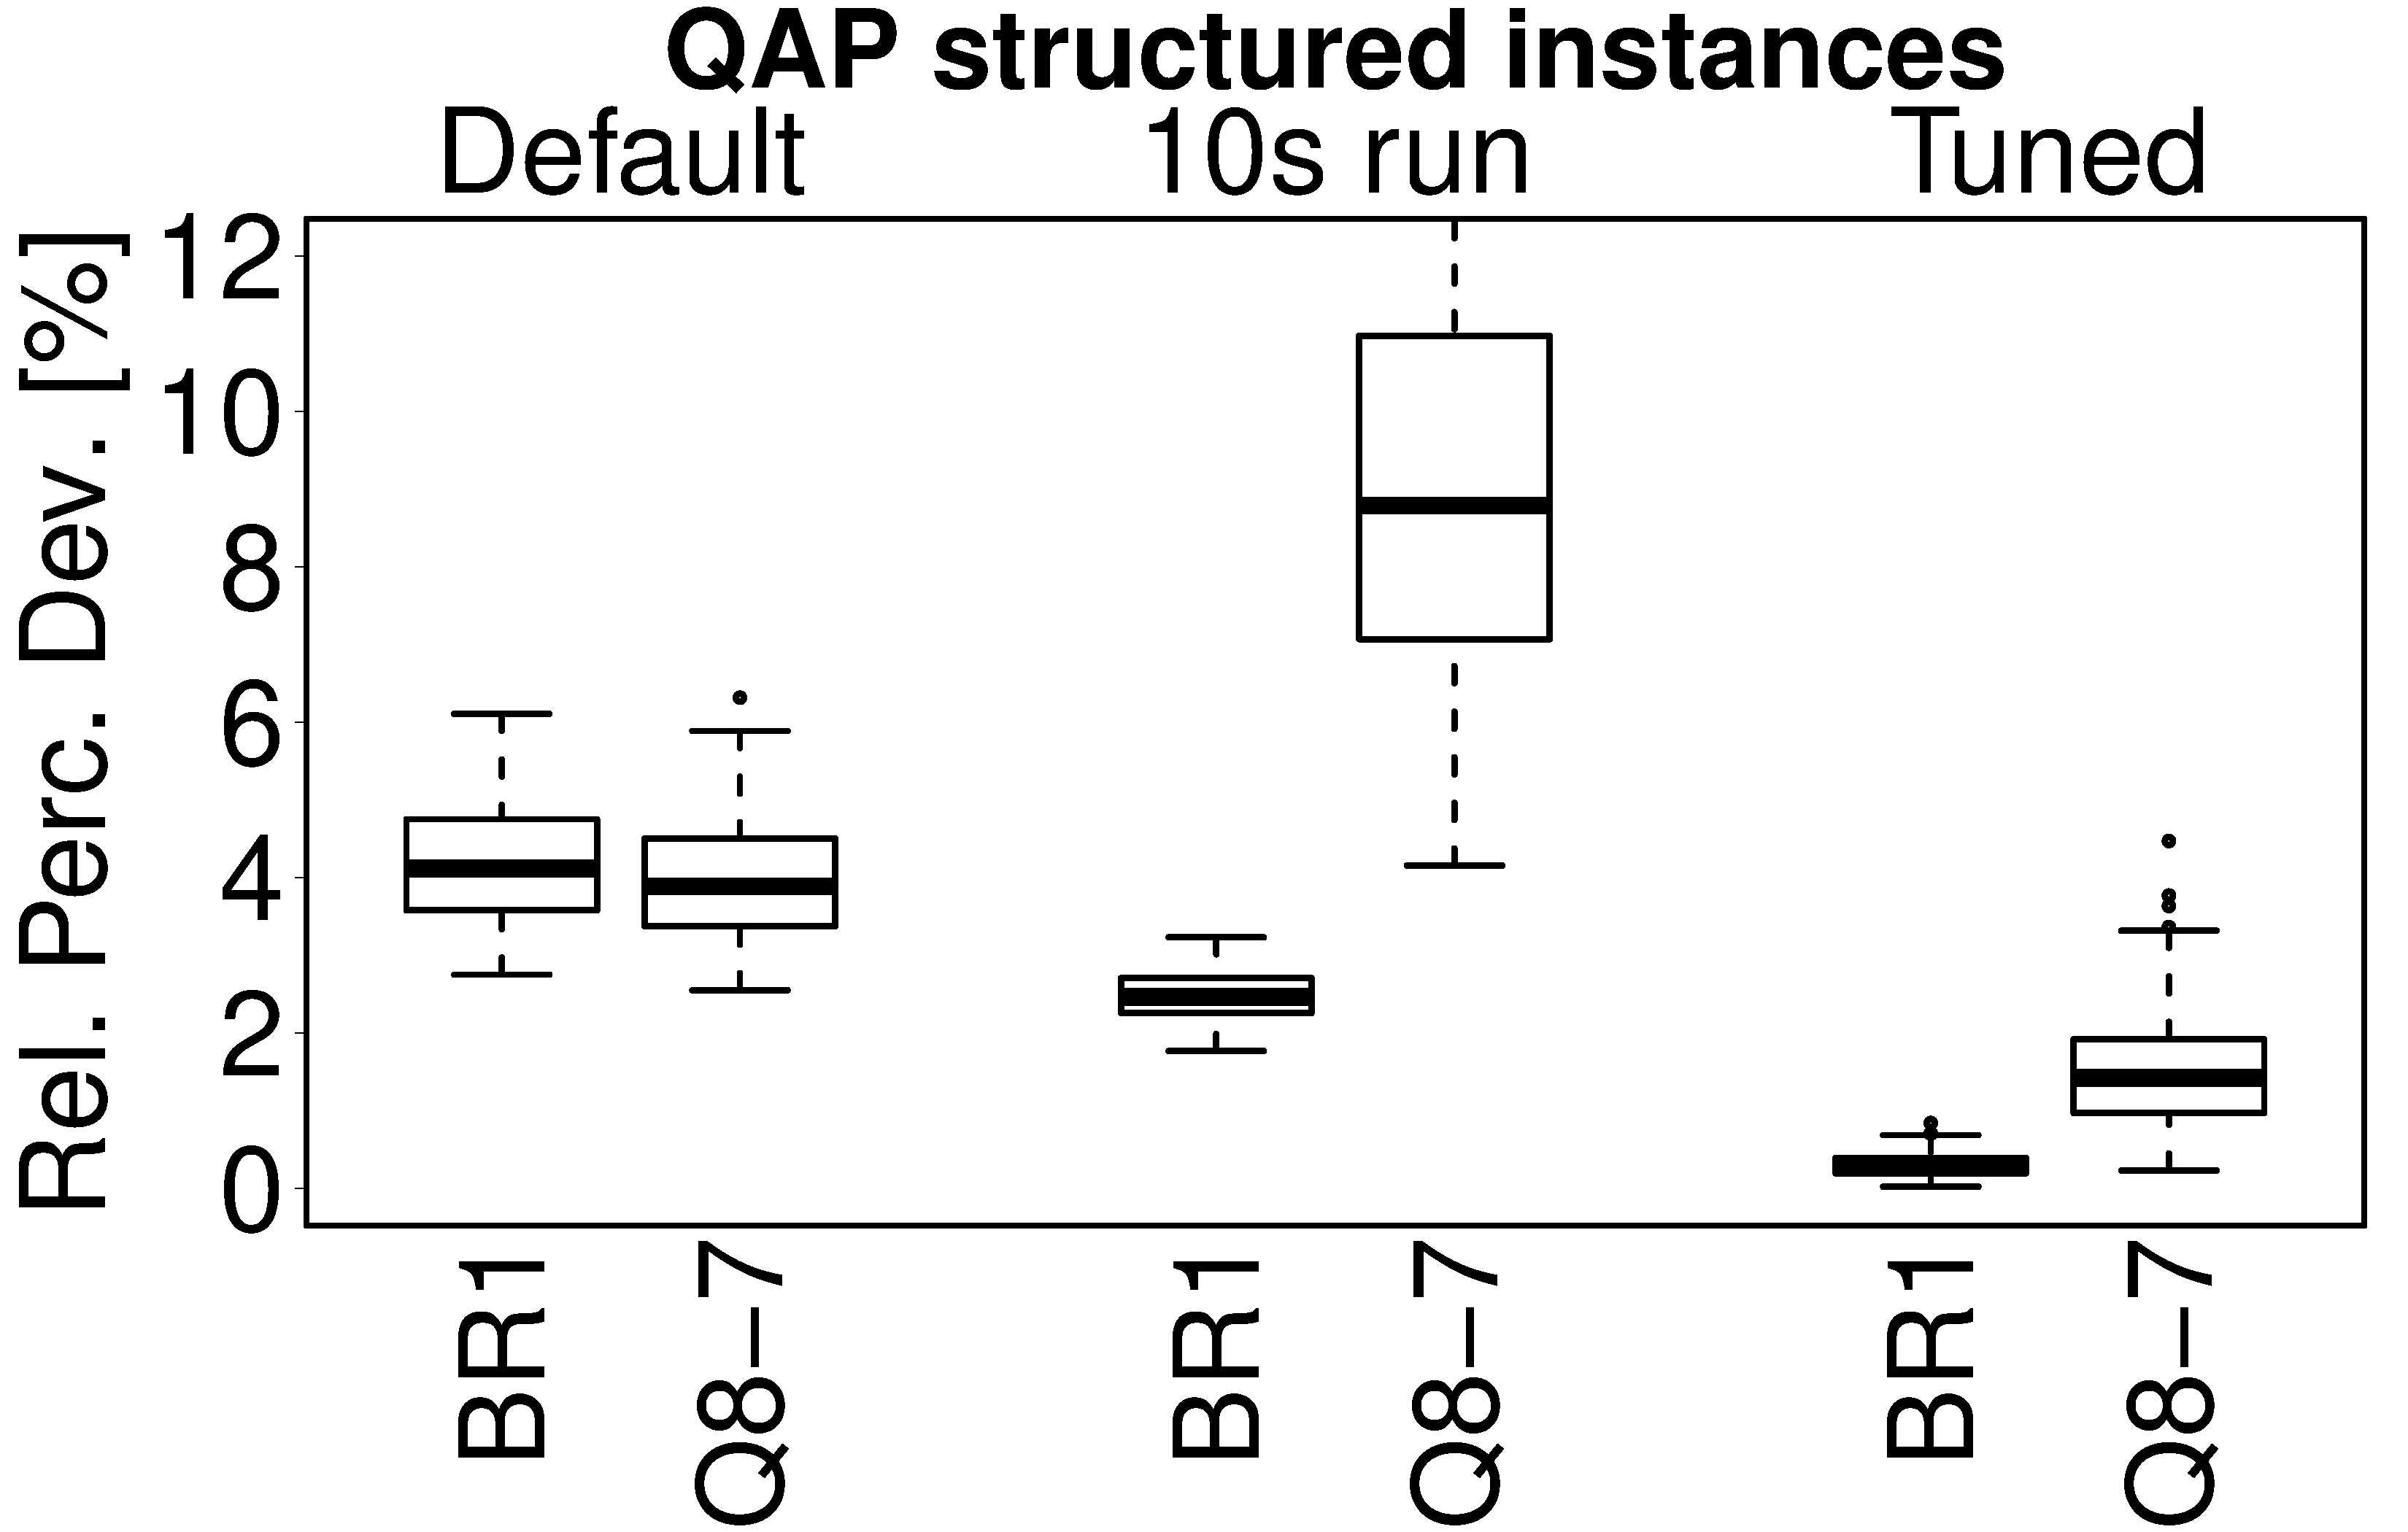
\includegraphics[width=0.49\textwidth]{Part 2 - Search-Based Optimization/Simulated Annealing/figures/es-bxp.pdf}
    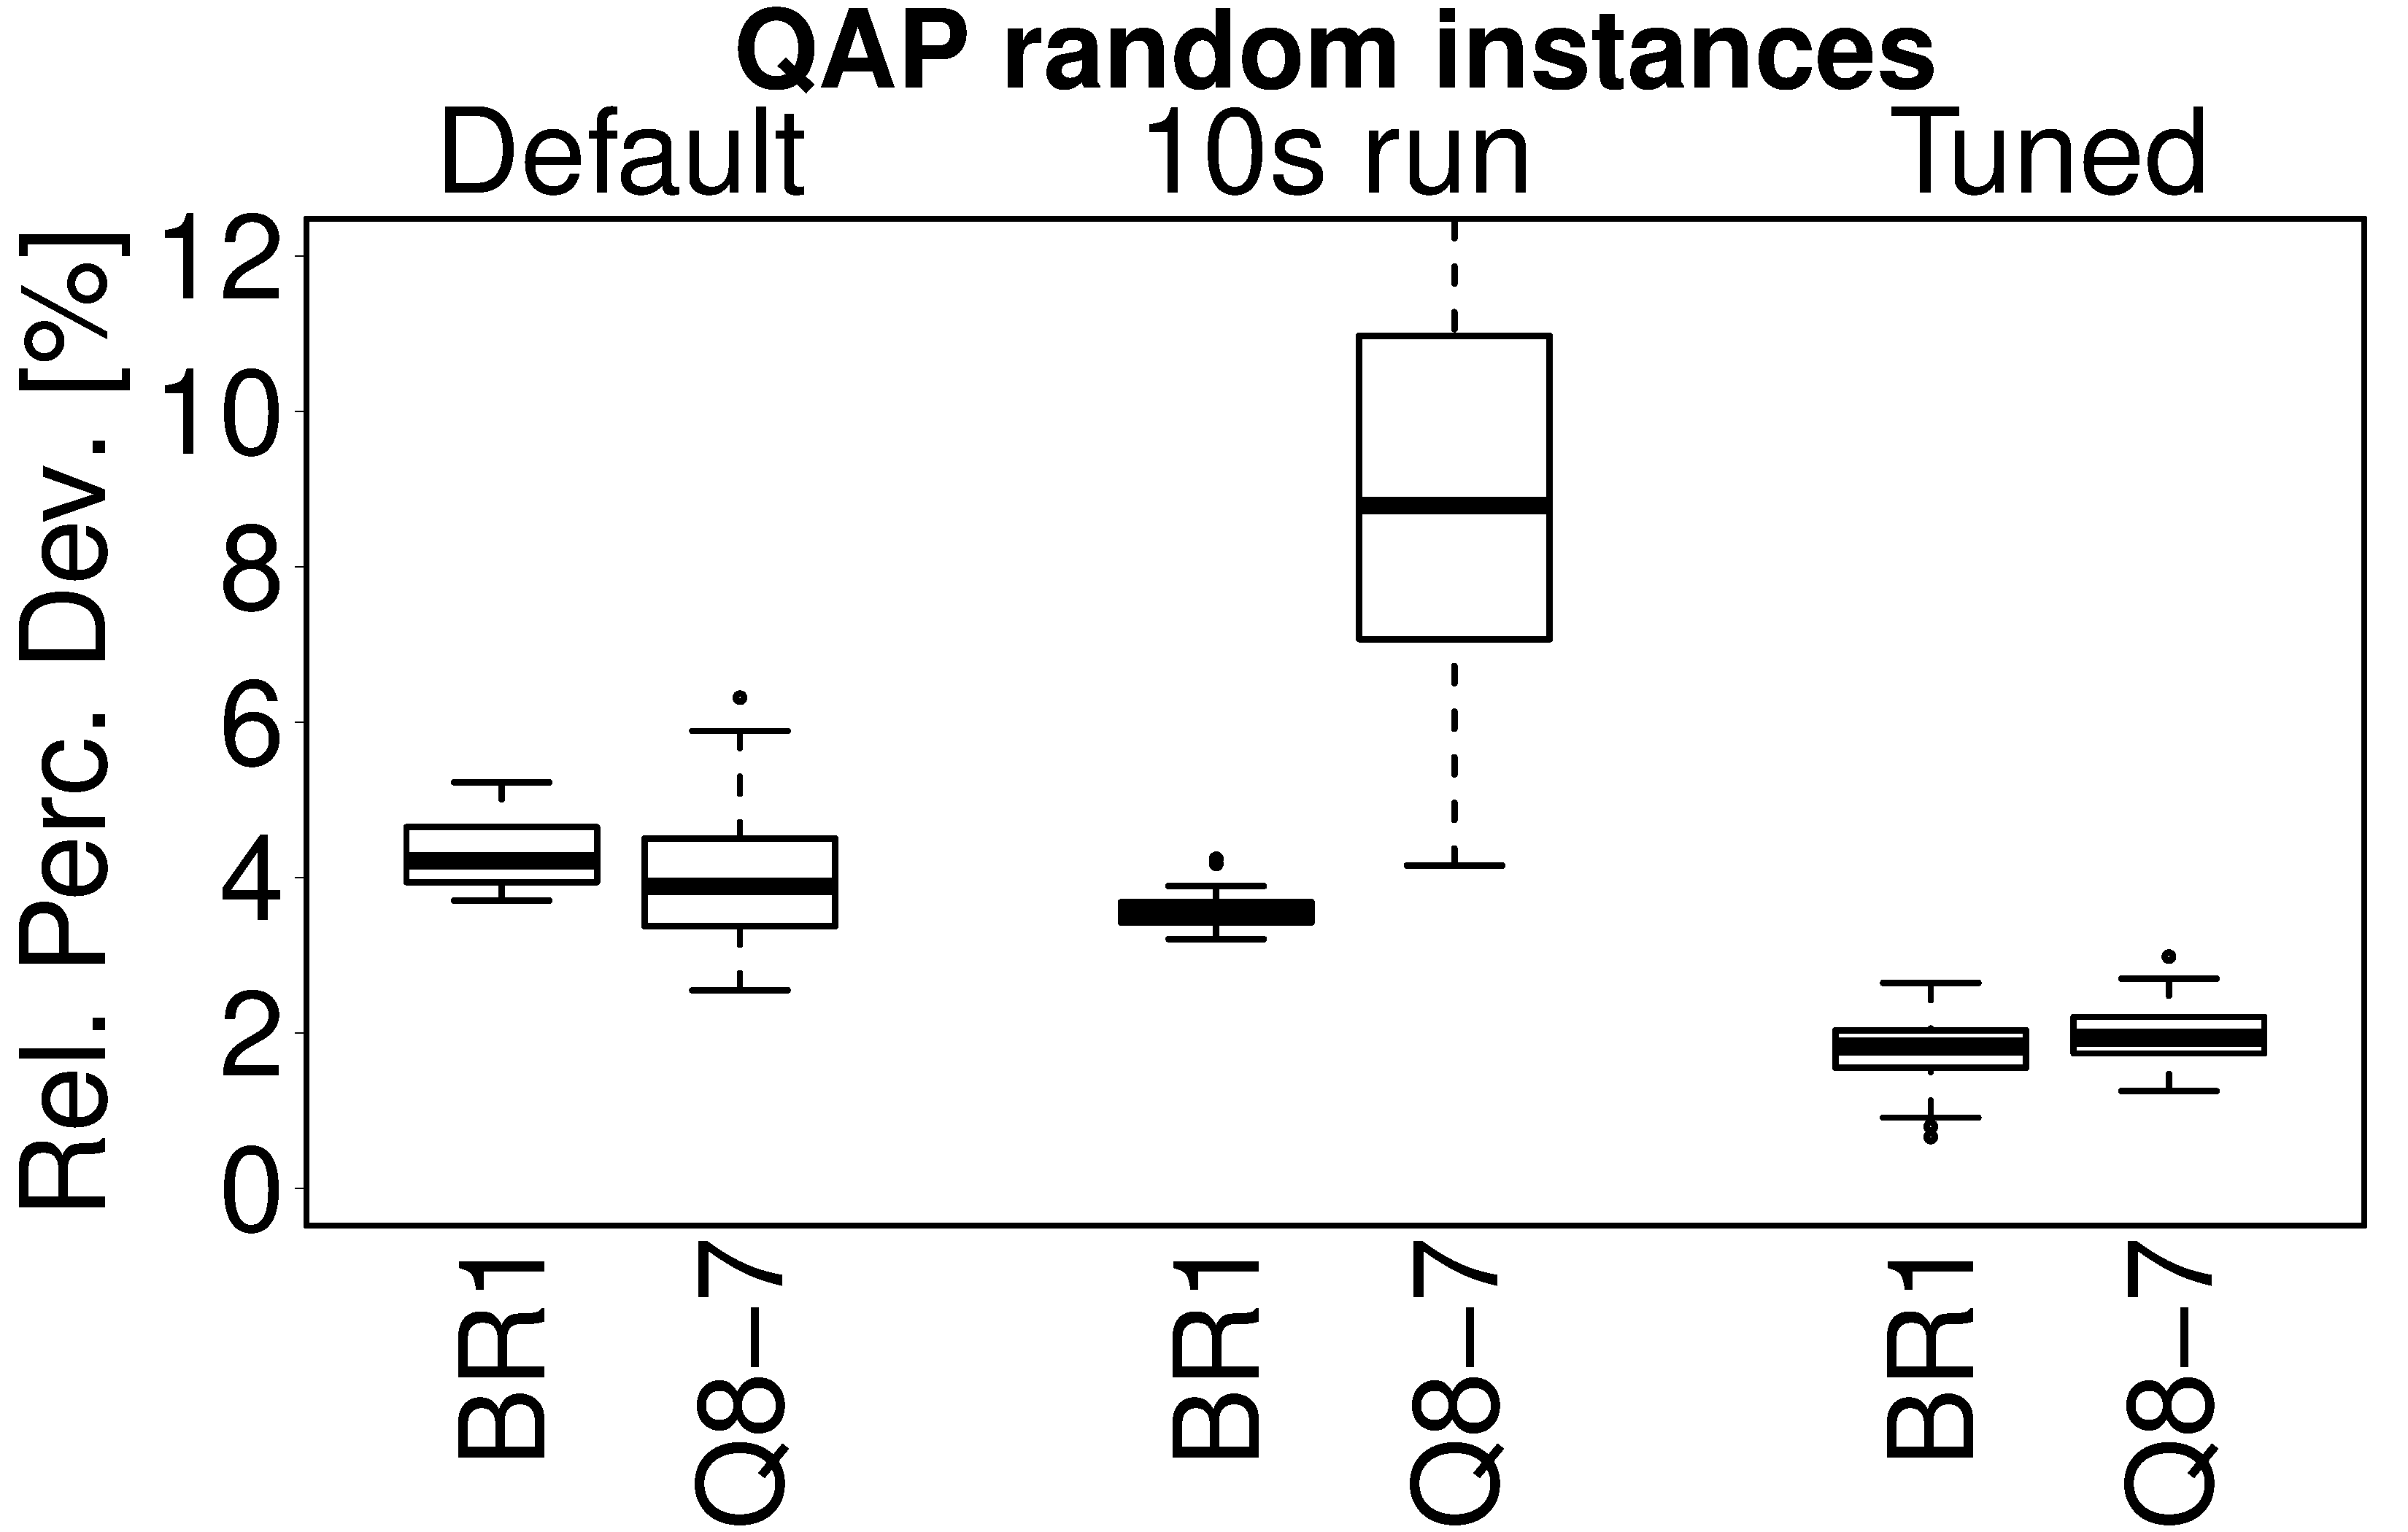
\includegraphics[width=0.49\textwidth]{Part 2 - Search-Based Optimization/Simulated Annealing/figures/rr-bxp.pdf}
  \end{center}
  \caption{Percentage deviation from the best known solutions obtained
  by the two simulated annealing algorithms on our structured
  and random QAP test set in their default settings, when let run for ten seconds,
  and when tuned using irace on a separate training set.}
  \label{fig:resqap1}
\end{figure}

In the first experiment the results obtained by \brsa and \qsa are similar, with a relative percent 
deviation (RPD) around $4\%$. This is because the algorithms are fairly old and 
most likely they have been manually
fine-tuned on small instances with little computational power available. 
If we let them run for a longer time, 
which can be done by simply replacing the termination condition,
this clearly favours \brsa that improves its results. 
The same modification has however a surprising effect on \qsa, which 
significantly worsens its results. This can be explained by considering 
how the Q8-7 cooling scheme is defined in the original paper. When 
this component is re-implemented exactly as described, one of the parameters
is computed relatively to the expected number of total move 
evaluations of the search. This value defines
therefore a delicate balance, that collapses if this value 
increases dramatically, as it is the case in our experiments. The resulting 
value makes therefore the temperature update too slow, and the algorithm
is unable to remain on good converging paths as it has a very high probability
of accepting worsening moves for a too large part of the search. 
We then tune the numerical parameters of the algorithms using irace, paying
attention to modifying the Q8-7 cooling scheme such that its parameters
can be independently configured. In this case, on both instance classes
both algorithms significantly improve their performance. 
On the structured instances, however, \brsa with an RPD of around $0.2\%$ 
clearly outperforms \qsa, which finds solutions on average worse than $1\%$ 
over the best known ones. On the random instances, instead, both algorithms obtain 
solutions on average just below $1\%$ of RPD, with \brsa marginally better than \qsa.

\begin{figure}[tb]
  \begin{center}
    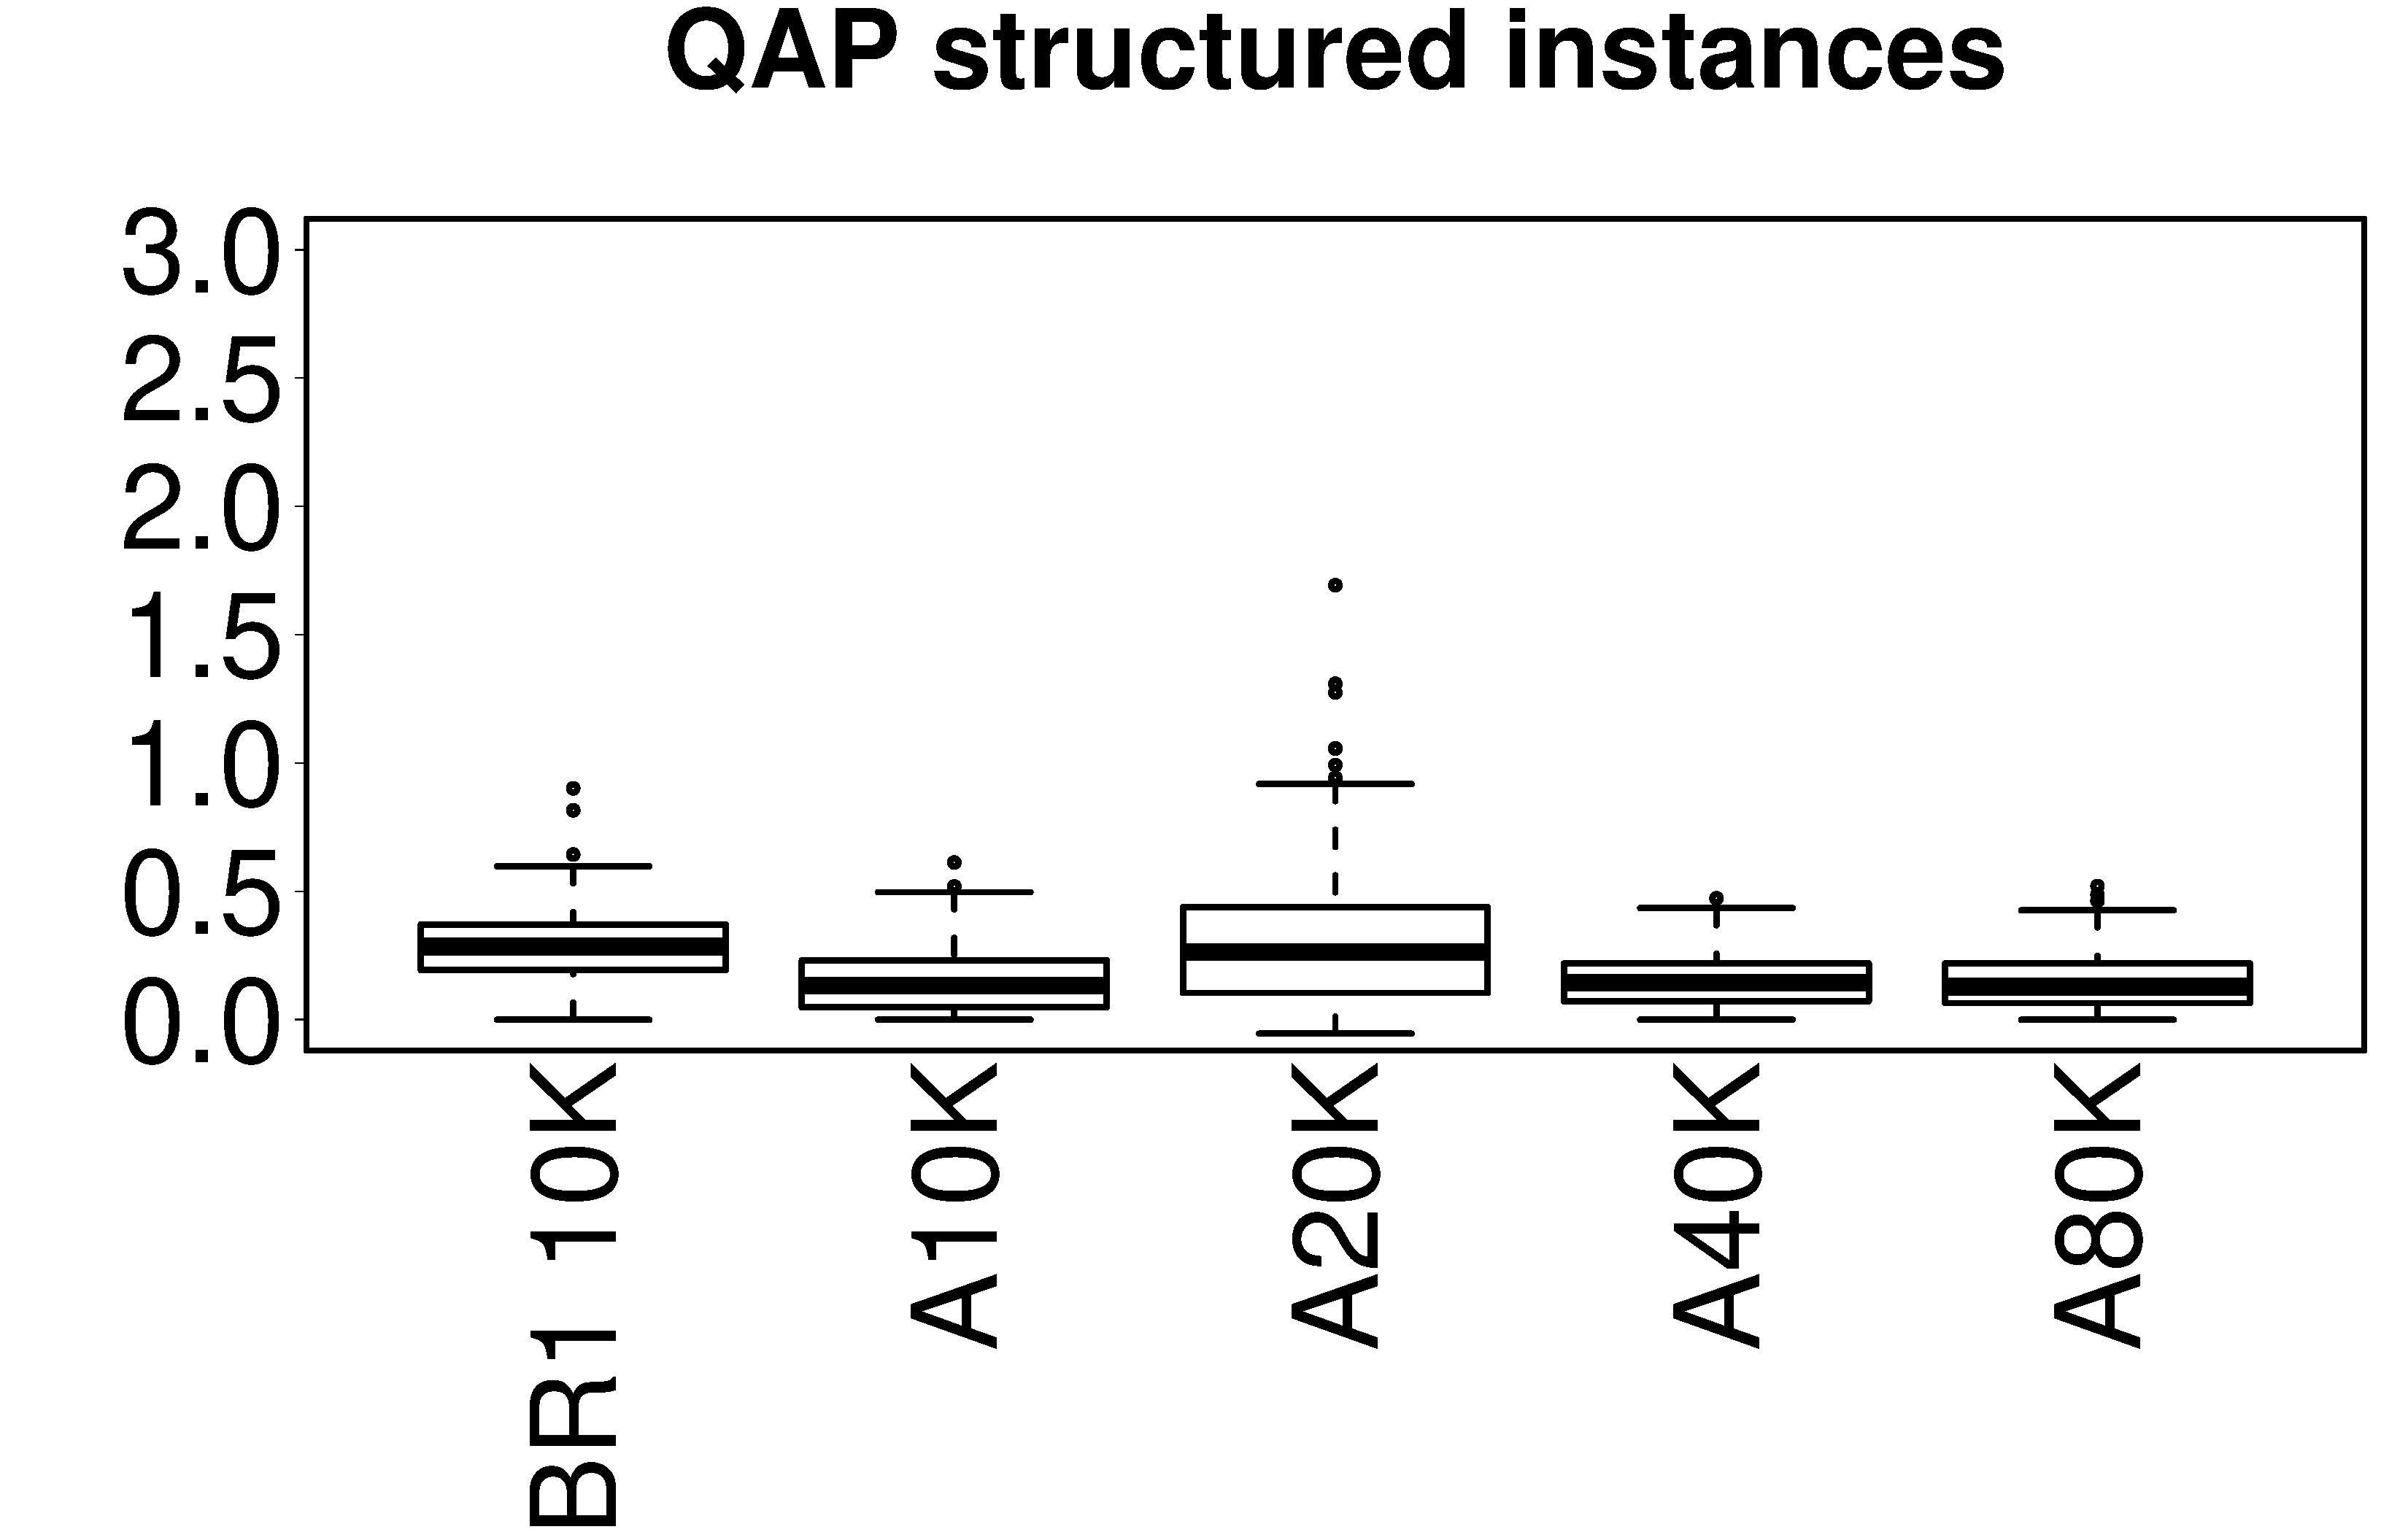
\includegraphics[width=0.49\textwidth]{Part 2 - Search-Based Optimization/Simulated Annealing/figures/esall-bxp.pdf}
    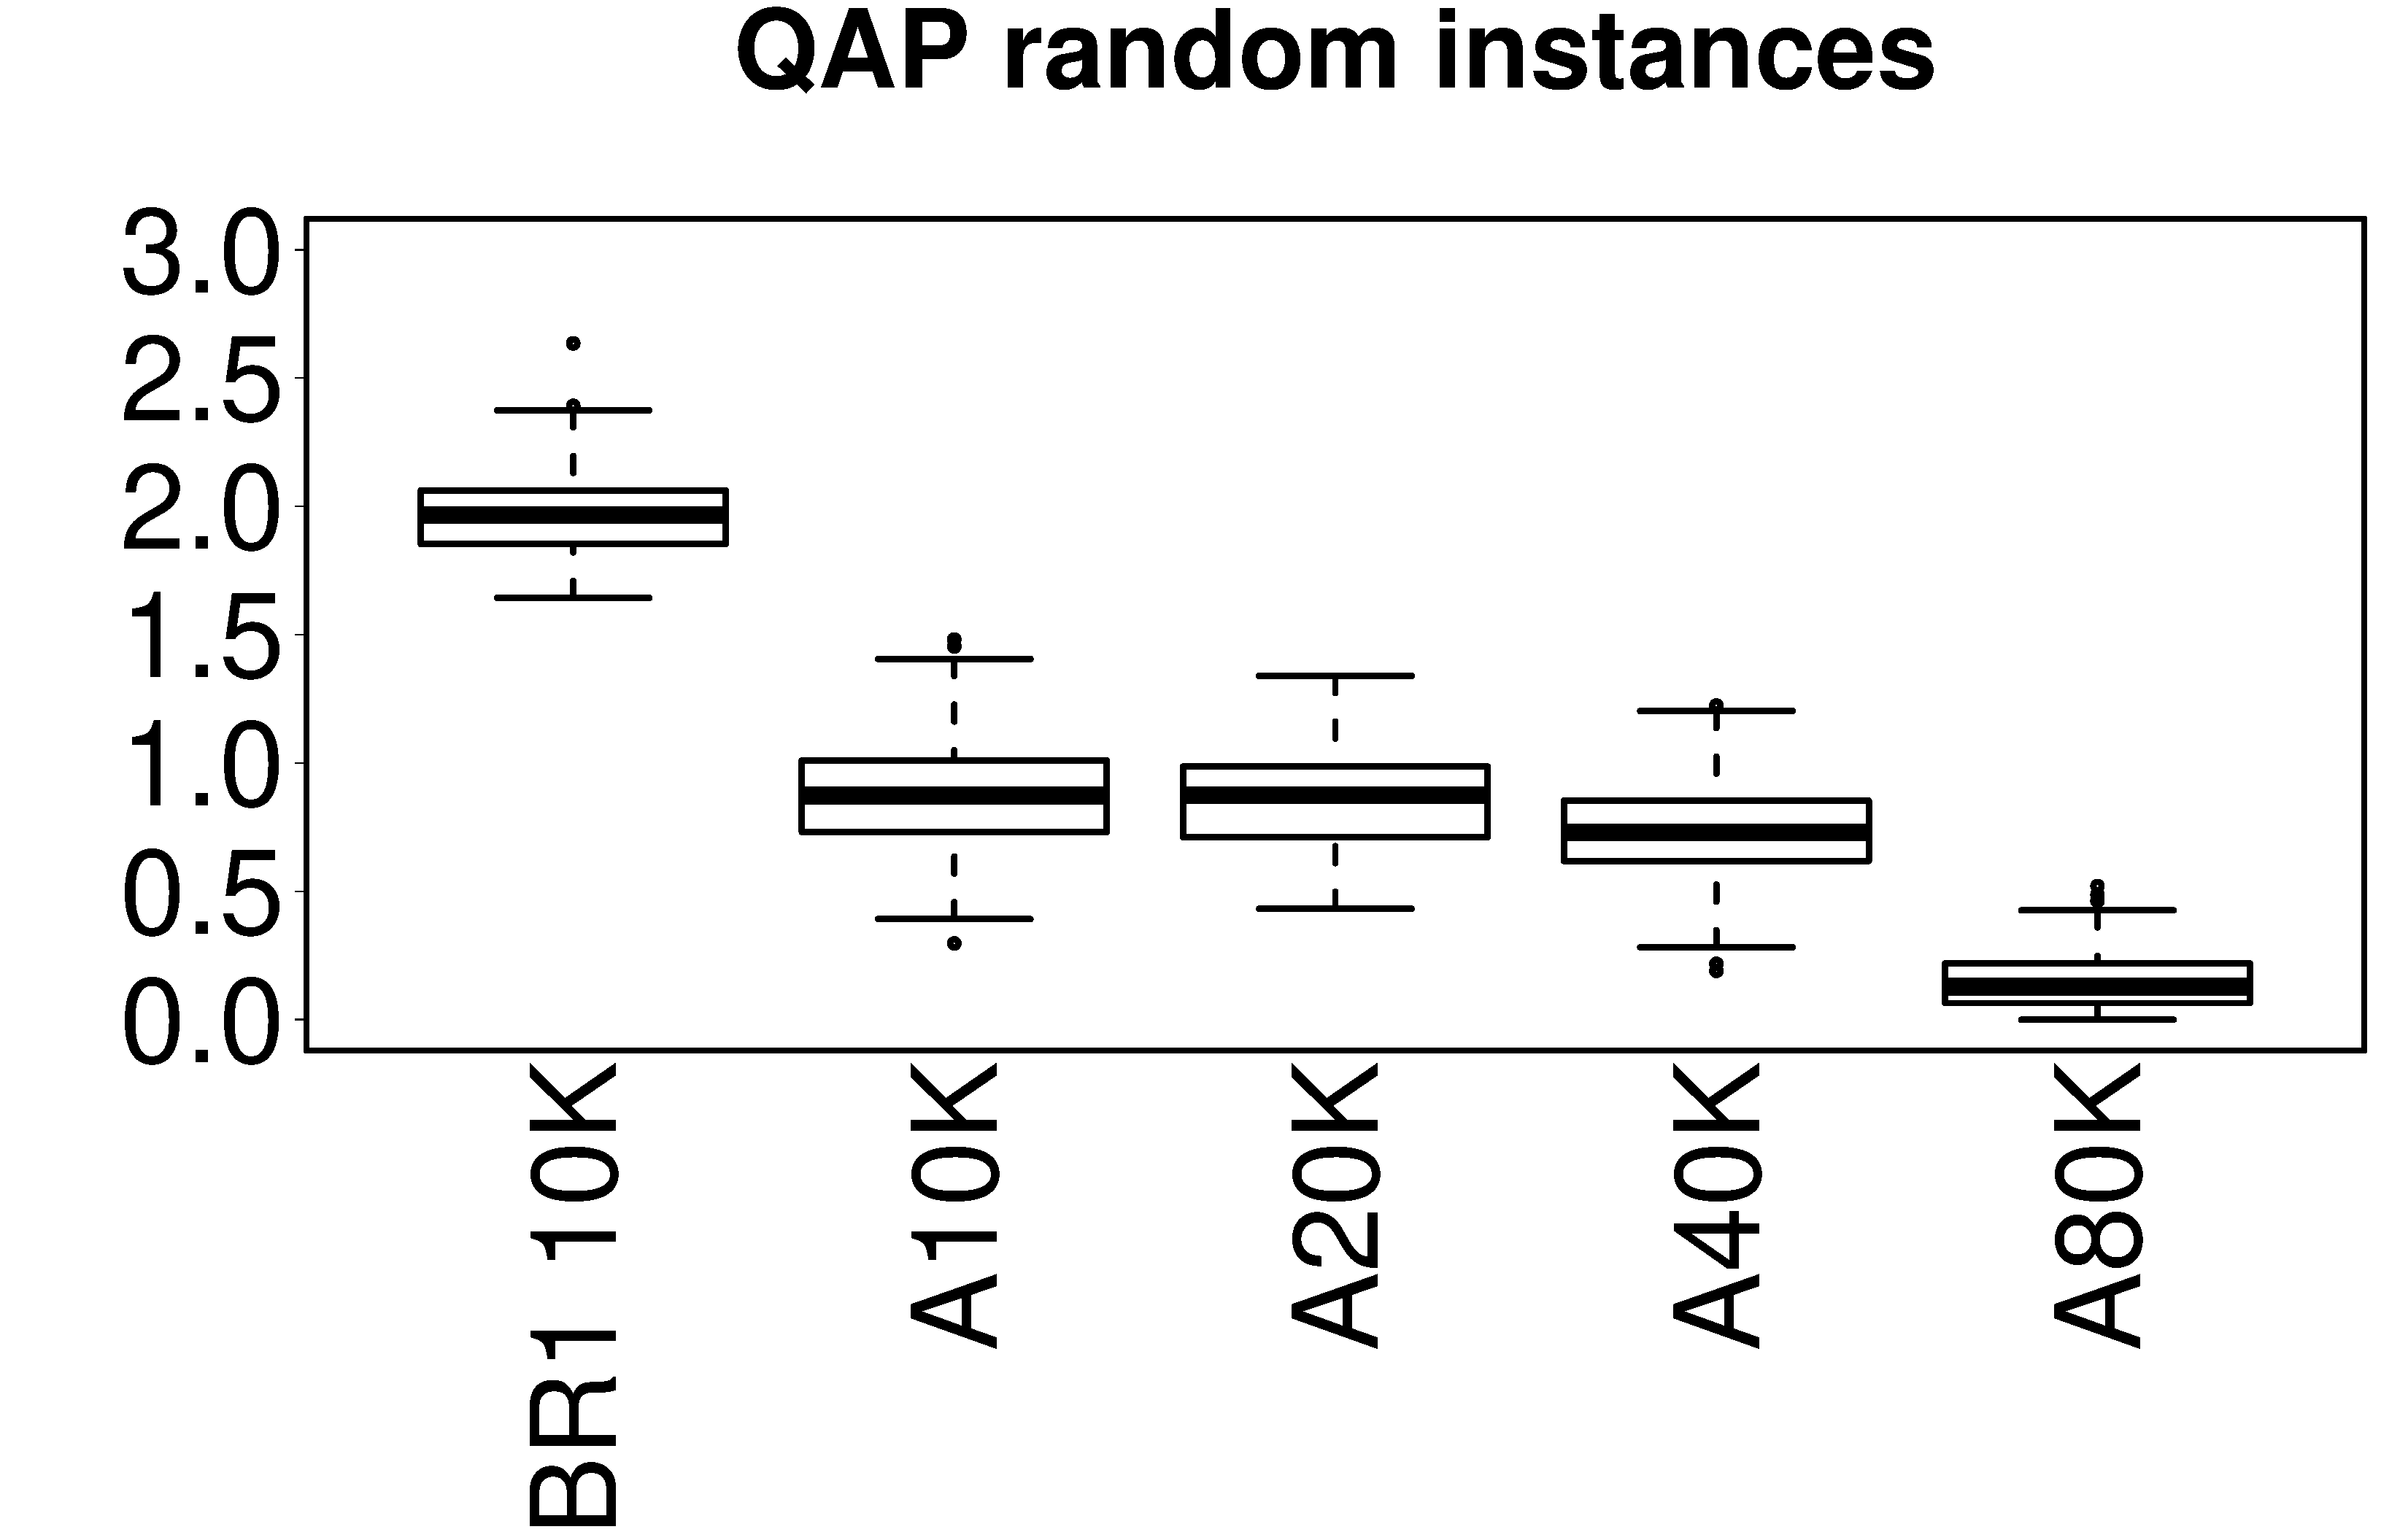
\includegraphics[width=0.49\textwidth]{Part 2 - Search-Based Optimization/Simulated Annealing/figures/rrall-bxp.pdf}
  \end{center}
  \caption{Percentage deviation from the best known solutions obtained
  when automatically designing simulated annealing algorithms from scratch using $10$K, $20$K, 
  $40$K and $80$K experiments on our structured and random QAP test set, compared
  with \brsa tuned with $10$K experiments.}
  \label{fig:res2qap}
\end{figure}


\subsubsection{Generating new algorithms}
Finally, we exploit the whole set of options identified in the literature
for the different simulated annealing components, using irace to automatically select
the best combination and thus design new algorithms from scratch. We report
in Figure \ref{fig:res2qap}
the results obtained by the algorithms that result from automated design tasks
with $10$K, $20$K, $40$K and $80$K experiments.
The algorithms obtained with the highest budget are reported 
in Algorithms \ref{algo:allsaes} and \ref{algo:allsarr} for 
structured and random instances, respectively.


\begin{algorithm}[ht!]
	  \caption{Component-based formulation of the SA automatically designed 
	  for the structured instances with a tuning budget of $80$ thousands experiments. 
	  The components are highlighted in \textit{italic}.}
     \label{algo:allsaes}
    
    Parameters: a problem instance $\mathcal{I}$, the \textit{$2$-exchange neighbourhood}, 
    \textit{a random permutation $\mathbf{x}_0$}, control parameters 
    $\theta = (p, 0.2249, k = 0.6969, \beta = 4645.392, \alpha = 0.6921, \gamma = 32)$
    
    Output: the best solution $\mathbf{x^*}$ found during the search.
    
	\begin{algorithmic}[1] 
		\STATE{$\textrm{best solution } \mathbf{x^*} := \textrm{incumbent solution } \mathbf{\hat{x}} := \mathbf{x}_0$\;}
		\STATE{$i := 0$\;}
        \STATE{Initialize temperature $T_0$ as \textit{the value that gives an expected initial acceptance probability $p$ of worsening moves in a random walk of length $l=10^4$, with a scaling factor $k$} \;}
		\WHILE{\textit{less than $10$ seconds of runtime}}
		\STATE{choose a solution $\mathbf{x}_{i+1}$ in the \textit{$2$-exchange neighbourhood} of $\mathbf{\hat{x}}$ \textit{at random}\;}
		\IF{$ \mathbf{x}_{i+1}$ meets \textit{Metropolis criterion}}
		\STATE{$ \mathbf{\hat{x}} := \mathbf{x}_{i+1}$\;}
		\IF{$ \mathbf{\hat{x}}$ improves over $\mathbf{x^*}$}
		\STATE{$\mathbf{x^*} :=  \mathbf{\hat{x}}$\;}
		\ENDIF
		\ENDIF
		\IF{\textit{the temperature value drops below} $\beta$}
		\STATE{update temperature according to \textit{geometric cooling with factor} $\alpha$\;}
		\STATE{reset temperature \textit{to initial value $\gamma$ times the neighbourhood size}\;}
		\ENDIF
		\STATE{$i := i + 1$\;}
		\ENDWHILE
        \STATE{return $\mathbf{x^*}$\;}
	\end{algorithmic}
\end{algorithm}


\begin{algorithm}[ht!]

	  \caption{Component-based formulation of the SA automatically designed for 
	  the random instances with a tuning budget of $80$ thousands experiments. 
	  The components are highlighted in \textit{italic}.}
     \label{algo:allsarr}
    
    Parameters: a problem instance $\mathcal{I}$, the \textit{$2$-exchange neighbourhood}, 
    \textit{a random permutation $\mathbf{x}_0$}, control parameters 
    $\theta = (k = 0.5438, \delta = 632, \alpha = 0.0.5927, \beta = 0.65, \gamma = 1208, r = 71822, s = 0.0828)$
    
    Output: the best solution $\mathbf{x^*}$ found during the search.
    
	\begin{algorithmic}[1] 
		\STATE{$\textrm{best solution } \mathbf{x^*} := \textrm{incumbent solution } \mathbf{\hat{x}} := \mathbf{x}_0$\;}
		\STATE{$i := 0$\;}
        \STATE{Initialize temperature $T_0$ as \textit{the average gap between consecutive solutions in a random walk of length $l=10^4$, with a scaling factor $k$} \;}
		\WHILE{\textit{less than $10$ seconds of runtime}}
		\STATE{choose a solution $\mathbf{x}_{i+1}$ in the \textit{$2$-exchange neighbourhood} of $\mathbf{\hat{x}}$ \textit{as the best one among $\delta$ randomly chosen ones}\;}
		\IF{$ \mathbf{x}_{i+1}$ meets \textit{Metropolis criterion}}
		\STATE{$ \mathbf{\hat{x}} := \mathbf{x}_{i+1}$\;}
		\IF{$ \mathbf{\hat{x}}$ improves over $\mathbf{x^*}$}
		\STATE{$\mathbf{x^*} :=  \mathbf{\hat{x}}$\;}
		\ENDIF
		\ENDIF
		\IF{\textit{exponentially increasing temperature length with parameters $r,s$} is met}
		\STATE{update temperature according to \textit{geometric cooling variant with factors} $\alpha, \beta$\;}
		\STATE{reset temperature \textit{to the one of the best solution found if no move accepted in the last $\gamma$ ones}\;}
		\ENDIF
		\STATE{$i := i + 1$\;}
		\ENDWHILE
        \STATE{return $\mathbf{x^*}$\;}
	\end{algorithmic}
\end{algorithm}

On the structured instances the results are slightly better than those obtained
by \brsa, with the exception of the configuration found with $20$K experiments.
This is a somewhat easy scenario, and it takes relatively little effort
to find good solutions. 
The random instances scenario is instead more challenging, and it takes 
more experiments to find a suitably good configuration. In fact, while
the tuning with $10$ thousand experiments improves a lot over \brsa,
it takes $40$ thousand experiments to marginally improve the results. Using
$80$ thousand experiments, however, it is possible to find configurations that
find solution qualities comparable to the structured instances case.

For different budgets, the results obtained on the structured instances
are very similar, and so are the algorithms. They all feature original simulated annealing components
such as the Metropolis acceptance, a geometric cooling scheme with cooling rates 
between $0.61$ and $0.83$ and a
random neighbourhood exploration.
There are instead different strategies for the temperature length and restart.
The initial temperature is defined in different ways, all of them relatively to 
some statistics computed during a preliminary random walk in the solution space. 
The algorithms obtained for the random instances are more different among each other.
The only common component is the Metropolis acceptance criterion. 
A closer inspection of the search trajectory reveals instead that
the algorithms effectively maintain the same or almost the same temperature value
for large portions of the search. In other words, the tuning process ends up shaping
a relatively complex algorithm that works like a very simple one. Our set of options
includes the possibility of maintaining the same temperature throughout the whole search, 
but it is more difficult to initially sample one with good settings, that has the chance of
surviving during the tuning.

The difference in the algorithms obtained can be explained with a closer
inspection to the landscapes traversed by the algorithms. On the random instances
the neighbourhoods have a distribution of solution values 
relatively similar to solutions in areas of different quality around the solution space, 
making this a scenario
that does not require variations of the algorithm parameters. On the 
structured instances, instead, neighbourhoods centered around average quality solutions
have different distributions of values than neighbourhoods around good solutions, and in this case
the flexibility of simulated annealing makes it more likely to adapt the algorithm to
the different areas of the landscape encountered \cite{IRIDIA-2021-005}.

It has to be noted that we considered only one tuning task for every budget, and
repeating each task with a different random seed may give algorithms that are different,
to a certain extent. At the same time, we have run the configuration tasks for the algorithm 
that has the full training set of 100 parameters for four different budgets. We commonly observe 
that a higher budget usually is good especially if the configuration tasks have many parameters. 
Anyway, one should observe that on the structured instances with 20K one has a relatively 
poor algorithm, 
something that can happen due to the stochasticity in the configuration process.



\section{Summary and Discussion}
\label{sec:conclusions}

In this chapter, we have seen how to implement a simulated annealing 
algorithm in terms of the design choices to make. 
We have shown how to combine the knowledge on algorithmic components 
and parameter settings  with automatic configuration tools 
to develop efficient simulated annealing
algorithms. This methodology is nonetheless general, 
and works for any stochastic local search method.
There are some inherent advantages 
for this such as making these components and parameters available for 
future use, allowing experimental analyses to identify the circumstances under which
every component will be most successful,
and exploiting directly the recent advances in the automatic 
configuration of algorithms.
This applies even more strongly when we want to design an algorithm that finds
good solutions as soon as possible, or, in other words, that exhibits a good 
\textit{anytime behaviour}. 

In the experiments we observed how good simulated annealing algorithms look 
like for different QAP instance classes.  
In general, in \cite{FraStu2019:cor} we have many more simulated annealing algorithms 
for the QAP identified and, independent of which simulated annealing we have, 
we found the automated configured simulated annealing with the variety of our settings 
always superior to these specifically designed algorithm for the QAP.
An importance analysis conducted across different problems and instance classes
indicated in fact that the acceptance criterion is the most important component in a
simulated annealing, followed by the neighbourhood exploration criterion. 
These two components are precisely the ones that operate locally in the neighbourhood.
In general, we have seen that different scenarios require different algorithms,
but even for the same scenario we may have different algorithms that perform 
equally well. 
Quantifying the appropriate diversification and understanding what algorithm 
could obtain the desired behaviour are anyway tasks 
better performed with the help of automatic tools. They can, in fact, 
select the best options for each algorithmic component and parameter, 
thus making the best out of the available body of knowledge that can be
found in the literature. 

A different approach is extending our approach to other stochastic local search methods and to 
generate extended frameworks. Ideally, these extensions would be 
generated within a same framework so that possibly rich hybrids 
among these methods may be generated. This would enable us to 
compare automatically designed simulated annealings against other automatically 
designed stochastic local searches, to study the role, impact and composition of 
simulated annealing algorithms when combined with or used as part of other 
stochastic local searches. Ultimately, we can try to understand 
when and how to move beyond the simulated 
annealing structure, to automatically design bottom up new methods without 
constraining them to a predetermined form.

\section{Exercise}\label{sec:exercise}
In addition to \brsa and \qsa, in the literature there are several papers
proposing SA algorithms for the QAP or for problems that can be modeled
as such. 
We propose an open-ended exercise to become acquainted not only with 
Simulated Annealing, but also with a component-based perspective
on stochastic local search algorithms, and its automatic optimization.
You can take inspiration from the Supplementary Material of this chapter\footnote{\supplementurlsa}, but you can also start with a new clean implementation.

\begin{enumerate}
    \item Choose a SA for the QAP to implement. You can start from the works we
    cited in this Chapter, or you can look for other SA algorithms.
    \item Identify the components of the algorithm you chose
    comparing it with against the template we provide in Section
    \ref{sec:sacomponents}, along with their numerical parameters.
    \item Understand how they interact: think about each of them as a separate
    function, and analyze which data can be considered \textit{input}
    and \textit{output}.
    Use the template given in Algorithm \ref{algo:simannealing} as a  
    reference to determine the flow of information among the components.
    \item Implement the algorithm, making sure you can specify the 
    numerical values as command line parameters. SA is
    a stochastic algorithm, so remember to
    make it possible to specify a random seed too.
    \item Run some tests on the instances we provide in the Supplementary
    Material\footnote{\supplementurlsa}. Use different random seeds and record the results
    you observe.
    \item Play with the numerical parameters, trying to find
    a parameter combination that performs consistently better than
    the original parameter values.
    \item Use irace and the templates
    provided in the Supplementary Material\footnote{\supplementurlsa} to automatically tune
    the numerical parameters \cite{LopDubPerStuBir2016irace}. 
    Re-run the tests, and observe the difference of results.
    \item If you feel brave, implement alternative components, such as
    new functions to update the temperature value, or to determine 
    whether to accept a candidate solution. You can take these ideas
    from existing papers, or come up with new components on your own.
    An implementation that reflects the component-based perspective
    of SA will make it way easier to observe the impact of your new
    components. You can even introduce a new command line parameter
    to add the choice at runtime.
\end{enumerate}

\section*{Acknowledgments}
Alberto Franzin acknowledges support from the 
Service Public de Wallonie Recherche under grant n\textdegree 2010235 - ARIAC by DIGITALWALLONIA4.AI.
Thomas St\"utzle acknowledges support from the Belgian F.R.S.-FNRS,
of which he is a Research Director. 

\bibliographystyle{unsrt}
\bibliography{bibliography}

\title{Differential Evolution}
\label{chp:differential-evolution}
\author{}
\institute{}
\maketitle


Add your content here


\bibliographystyle{unsrt}
\bibliography{bibliography}

\title{Particle Swarm Optimization}
\label{chp:particle-swarm-optimization}
\author{Diego Oliva, Alfonso Ramos-Michel, Mario A. Navarro, Eduardo H. Haro, Angel Casas}
\institute{Universidad de Guadalajara, CUCEI}
\maketitle

%\textbf{Abstract}\\
%Particle swarm optimization (PSO) is one of the most important meta-heuristic algorithms. It serves as a base for modern methods and has been applied in several fields. Its importance is due to its simplicity and collective behavior that permits finding the optimal solutions to complex problems. The popularity of the PSO also permits researchers to design different variants that improve its performance. This chapter analyzes the importance of the PSO as an intelligent algorithm. Here are presented the basic concepts of the PSO, some examples, and a study of the most important variants and applications. The idea is to provide the reader with an overview of this interesting approach.


%This file lists some brief information about how optimization problems are going to be defined in the IEEE CIS Open Book. We ask your book sections to follow the notations listed here for consistency. If you have any questions regarding the notation, please contact Leandro Minku (l.l.minku@bham.ac.uk). 

%Please use the svmult style file and follow Springer's svmult guidelines, which can be downloaded here: \url{https://www.springer.com/birkhauser/mathematics?SGWID=0-40292-2-122598-0}. Please use the ruled and graybox options of the style file.

%Section \ref{sec:intro} presents the notation for machine learning. Section \ref{sec:optimization} presents the notation and some definitions for optimization. Section \ref{sec:alg} presents the notation for pseudocode. Example citations are as follows: \cite{KocaguneliEtAl2013}, \cite{KocaguneliEtAl2013-2}.

%We also ask authors to adopt American spelling for the English language used in the sections, if possible. 


%\hfill
%\section{Introduction}
%\label{sec:intro}

Nature is the source of inspiration for different processes in science and engineering. Since nature is an example of the world, humans have tried to imitate different behaviors over the years. This occurs not only in a personal way but also happens in the creations and constructions. The collective behavior that is present in an animal that lives in groups is a clear example of how nature solves the problem of finding sources of food, shelters, or places to migrate. In the case of food sources or hunting, a group is more capable of finding food than a single animal. This means that with more members of the group have more probability of catching prey. 

In computer sciences, intelligent algorithms' design could be seen as an attempt to imitate nature. In this sense, techniques such as Particle Swarm Optimization (PSO) is an example of inspiration from nature as a base to solve complex problems \cite{kennedy1995particle}. The PSO is part of a group of methods called meta-heuristic algorithms that are widely important in artificial intelligence and applied mathematics. Meta-heuristic algorithms can use a biological, physical, or social phenomenon as a source of inspiration and provide the basis for modeling operators to perform optimization.

The PSO was initially proposed by Kennedy and Eberhart in 1995. It was developed to simulate the unpredictable choreography of birds flocking, but later it was used to solve many problems defined discrete-valued spaces where the domain of the variables is infinite \cite{kennedy1995particle}. Nonetheless, particle swarm optimization has attracted the scientific attention of miscellaneous engineering and physics areas; this is because there are several fields of study where it is necessary to find better solutions according to specific established criteria. Some other classical optimization approaches cannot be used in these types of problems because they could get caught in local optima \cite{janeza2009pso}. Even though particle swarm optimization has some similarities with genetic algorithms and other optimization approaches, the main difference is that instead of using mutation/crossover operators, it uses the global communication and real-number randomness as the swarm particles \cite{yang2010nature}.

The PSO works with a population of candidate solutions that are called particles. Each particle of the population collaborates with its search strategy to improve the quality of the solutions. In the early research related to PSO, we can see that the operators move the population as birds flock or school of fishes. PSO is then a simple optimization algorithm that allows to explore a search space and find the optimal solution. Due to its simplicity, PSO is a popular method, and it has been applied in different domains, from benchmark optimization problems to medical applications \cite{shi2001particle}. PSO has been studied by researchers over the years not only to use it for solving complex problems but also to understand how this algorithm works and to validate its performance from theoretical and empirical points of view \cite{shi1999empirical}. PSO is considered a powerful tool for optimization, and it is a classical approach that helps to inspire other algorithms such as swarm intelligence \cite{eberhart2001swarm}. However, PSO, like many other algorithms, has some drawbacks; for example, it could be trapped in sub-optimal solutions in complex search spaces (multi-modal problems). In this sense, in the related literature, they are more than 100 modifications of the PSO, and their modification is still growing every year \cite{imran2013overview}.

The popularity of PSO is reflected in the number of cites and publications indexed in different databases like Scopus. Figure~\ref{fig:PSOyear} shows a plot extracted from Scopus related to PSO from 2010 to 2021. From this graph, it is possible to see that in 2010 they were around 4000 documents published, and in 2020 the number of publications was between 8000 and 9000.

\begin{figure}[h!]
  %\vspace*{-.2cm}
  \centering
  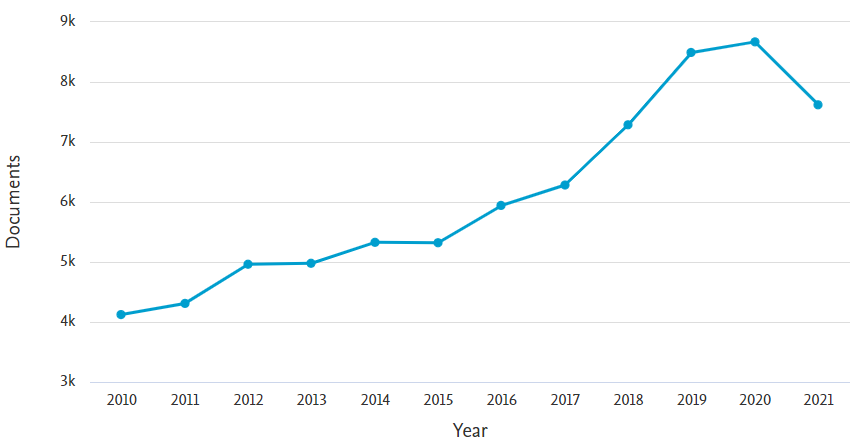
\includegraphics[scale=0.5]{"Part 2 - Search-Based Optimization/Particle Swarm Optimization/Images/PSO Year.PNG"}
  %%\vspace*{-.4cm}
  \caption{Number of articles per year of PSO between 2010 and 2021. \label{fig:PSOyear}}
  %\vspace*{-.3cm}
\end{figure}


%The modifications of PSO are also part of this case in the computer science or engineering field. 
To graphically show where the PSO impacts in the last ten years Fig.~\ref{fig:PSOarea}  presents a pie chart. The main field of application is engineering, followed by computer sciences, and third place in mathematics.

\begin{figure}[h!]
  %\vspace*{-.2cm}
  \centering
  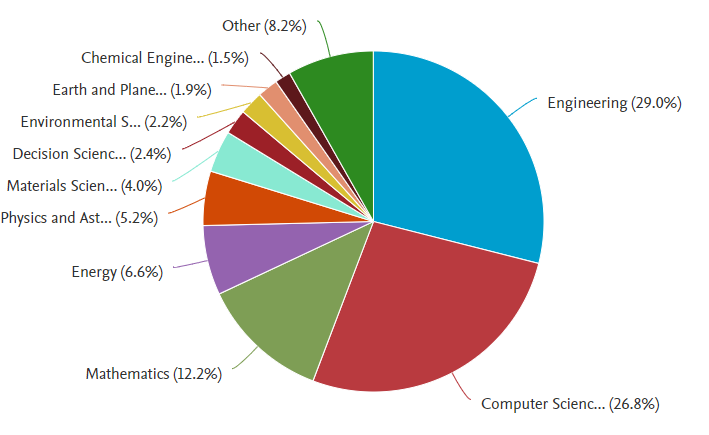
\includegraphics[scale=0.5]{"Part 2 - Search-Based Optimization/Particle Swarm Optimization/Images/PSO Area.PNG"}
  %%\vspace*{-.4cm}
  \caption{Documents by subject area related to PSO between 2010 and 2021. \label{fig:PSOarea}}
  %\vspace*{-.3cm}
\end{figure}

In this chapter, an introduction to the PSO algorithm is given. The goal is to provide an overview of the PSO, explain its basic concepts and operators, and present examples and exercises. Besides, the variants of the PSO are also discussed based on their importance in the scientific community. In the same context, they also studied the most important application of this vital algorithm.

The rest of the chapter is organized as follows: Section \ref{sec:psobasics} explains the operators of the PSO. Section \ref{sec:variants} discusses the main modification of the PSO. In Section \ref{sec:apps} are analyzed the most important PSO applications. Finally, Section \ref{sec:conclusions} discuses some conclusions and proposes some exercises.
%\todo[inline]{ DIEGO}
%Supervised learning: consider a set of examples 

%\[\mathcal{T} = \{(\mathbf{x}^{(1)},y^{(1)}),(\mathbf{x}^{(2)},y^{(2)}),\cdots,(\mathbf{x}^{(N)},y^{(N)})\}\]

%\noindent where $(\mathbf{x}^{(i)},y^{(i)}) \in \mathcal{X} \times \mathcal{Y}$  are drawn i.i.d. (independently and identically distributed) from a fixed albeit unknown joint probability distribution $p(\mathbf{x},y)$.

%Supervised learning aims at building a (predictive) model able to generalise to unseen (test) examples of the same probability distribution $p(\mathbf{x},y)$. In classification problems, $\mathcal{Y}$ is a set of categories / classes. In regression problems, $\mathcal{Y}$ is $\mathbb{R}$.

%Supervised learning aims at learn a (predictive) model able to generalise to unseen (test) examples of the same probability distribution% $p(\mathbf{x},y)$. In classification problems, $\mathcal{Y}$ %is a set of categories / classes. In regression problems, $\mathcal{Y}$ is $\mathbb{​R}$.


%Mathematical notations:
%\begin{itemize}
%\item Scalar: lower case, e.g., $a$, $b$.
%\item Column vector: lower case, bold, e.g., $\textbf{x}$.
%\item Vector element: lower case with subscript, e.g., $x_1$, $x_2$.
%\item Matrix: upper case, bold, e.g., $\textbf{X}$.
%\item Matrix element: upper case with subscripts, e.g., $X_{1,2}$.
%\item If enumerating these (e.g., having multiple vectors), superscript will be used to differentiate this from indices, e.g., $\textbf{x}^{(1)}$, $\textbf{x}^{(2)}$.
%\item Use mathcal font for sets, e.g., $\mathcal{T}$ for training set.
%\end{itemize}

%Terms to be adopted:
%\begin{itemize}
%\item Please use the term ``input variable'' instead of ``independent variable'' or ``input attribute''.
%\item Please use the term ``output variable'' instead of ``dependent variable'' or ``output attribute''.
%\item Please use the term ``example'' instead of ``observation'', ``data point'' or ``instance''.
%\end{itemize}
 

%\newpage
\section{The fundamentals of PSO algorithm}
\label{sec:psobasics}

This section introduces the basic concepts of the standard PSO and how it works. The pseudocode is described easily, and an example permits an analysis of the behavior of the algorithm.

\subsection{The PSO structure}

Essentially, each particle in the swarm (which is considered a candidate solution) is randomly distributed and represented by a vector in a multidimensional search space; all this set of particles is considered the initial population. Once established the initial population, PSO searches for optima by updating each particle according to notions such as position, velocity, inertia, etc. These notions can be defined as a vector usually called \textit{the velocity vector}, which helps to determine the next movement of the particle. Nonetheless, this movement is not entirely random; each particle is attracted towards both its own personal best position and the best position of the swarm. Then, the population is evaluated in the objective function to determine the population quality. This also allows finding the best element that will be defined as a criterion to beat in the subsequent evaluation. The new generated positions of the particles and the speed with which they are moving are calculated considering the value of the best global element and the actual value of every particle compared with a random number \cite{erick2021matlab}.\\

When the population is initialized and evaluated, the particle with the lowest or highest objective value is obtained depending on whether it is a minimization or maximization problem, respectively. This found particle is called \textit{the global particle} $gB$. On the other hand, in each iteration of the algorithm, the current particle is compared with the newly generated particle; in other words, particles have to be evaluated in the objective function every time they are moved. If the generated particle is better than the current one, then it is replaced by the new particle, receiving the usual name of \textit{the actual best particle} $lB$. The general pseudocode of the particle swarm optimization algorithm is shown in Algorithm~\ref{alg:PSO}. In contrast, the phases of initialization and movement of particles that compose the PSO are explained in the following two subsections.\\

In order to better understand the pseudocode shown in Algorithm~\ref{alg:PSO}, it is enough to appreciate that it is divided into two main parts, the unnumbered part and the numbered part. The unnumbered part refers to those terms that the algorithm requires in order to perform its operation, terms such as the population number, dimensions, etc. Once the previous points have been established, the numbered part is given, which begins with the initialization of the population and its respective evaluation. The terms ``repeat" and ``until" refer to the beginning and end of the while loop, which is the main body of the algorithm.

\begin{algorithm}[h!]
\caption{Particle swarm optimization pseudocode}
Parameters $\rightarrow$ Dimensions, Bounds, Maximum iteration number, Number of particles.\\
Output $\rightarrow gB$.   
\begin{algorithmic}[1]
\STATE{Initialize the particles of population.}
\STATE{Evaluate the objective function.}
\REPEAT
\FOR{All particles in all dimensions}

\STATE Generate a new velocity.
\STATE Calculate a new position.
\STATE Evaluate again the objective function.
\ENDFOR
		
\STATE Update the best particle of population.
\UNTIL the maximum number of iterations is reached.
\end{algorithmic}
\label{alg:PSO}
\end{algorithm}

\subsubsection{Initialization of the PSO}

All meta-heuristic algorithms have an initialization phase that has the primary purpose of creating the initial population, where each particle represents a candidate solution for the optimization problem. These particles are randomly generated in a search space, which is delimited by the established bounds. Generally, the initialization phase also defines the parameters of the problem to optimize \cite{erick2021matlab}. The initialization of the PSO algorithm is defined by Eq.~\ref{eq:equation1}, which describes the optimization of its individual particles.

\begin{equation}
\vec{x}_{i,j}^t=lb_j+rand(ub_j-lb_j)
\label{eq:equation1}
\end{equation}

\noindent where $\vec{x}_{i,j}^t$ is the $i-th$ population particle, $i \in \{i=1,2,3,...,N\}$ represents the index of a given particle, $N$ is the maximum number of particles, $j$ represents the $j_{th}$ dimension of the design variable, where $0<j\leq d$ and $d$ is the dimensionality of the design variable. The iteration number is represented by $t$. While $lb_j$ and $ub_j$ define the lowest and upper limit, respectively. It is worth saying that $rand$ is a uniformly distributed random number between $0$ and $1$. Once established the respective position of each particle, it is necessary to define the velocity each one of them will move around the search space to find the global optimal. We will explain that phase next.

\subsubsection{Velocity and movement of particles}

To find the velocity, it is necessary to get the best global and local values of each particle, commonly called $\vec{gB}^t$ and $\vec{lB}_i^t$ respectively. Eq.~\ref{eq:equation2} defines the velocity calculation for each particle $i$:

\begin{equation}
\vec{v}_i^{t+1}=w \times \vec{v}_i^{t}+c_{1} \times \vec{r1}_i^t \times (\vec{lB}_i^t-\vec{x}^{t}_i)+c_{2} \times \vec{r2}_i^t \times (\vec{gB}^t-\vec{x}^{t}_i)
\label{eq:equation2}
\end{equation}

\begin{equation}
\vec{x}_i^{t+1}=\vec{x}_i^{t}+\vec{v}_i^{t+1}
\label{eq:equation3}
\end{equation}

\noindent where $\vec{v}_i^{t+1}$ is the particle $i$'s velocity of the iteration $t+1$, $\vec{v}_i^{t}$ is the particle $i$'s velocity in the previous iteration, the vector that contains each particle $i$'s position is $\vec{x}_i^{t}$ and $\vec{r1}_i^t$ and $\vec{r2}_i^t$ represent $d$-dimensional vectors containing uniformly distributed random numbers between $0$ and $1$. It is worth to say that $c_{1}$ and $c_{2}$ are called learning coefficients, and $w$ represents an inertia weight that affects the convergence and exploration-exploitation trade-off in PSO process. Since inception of inertia Weight in PSO, a large number of variations of Inertia Weight strategy have been proposed, nonetheless, it is generally established as 1. Meanwhile, Eq.~\ref{eq:equation3} is used to displace the particles to new positions in the next iteration. Where $\vec{x}_i^{t+1}$ is the vector where the new obtained position of particle $i$ at iteration $t+1$ is stored, $\vec{x}_i^{t}$ corresponds to the previous position of particle $i$ calculated at iteration $t$, and finally $\vec{v}_i^{t+1}$ is the velocity vector obtained by Eq.~\ref{eq:equation2}.

It is essential to mention that the majority of modifications to the PSO algorithm have as purpose to find new ways to accelerate the particles as best as possible \cite{erick2016optimizacion}. To end this section, Fig.~\ref{fig:PSOmovement} shows a graphic description of particle's velocity and their movement in the particle swarm optimization algorithm for a better understanding by the reader.\\

\begin{figure}[h!]
\centering
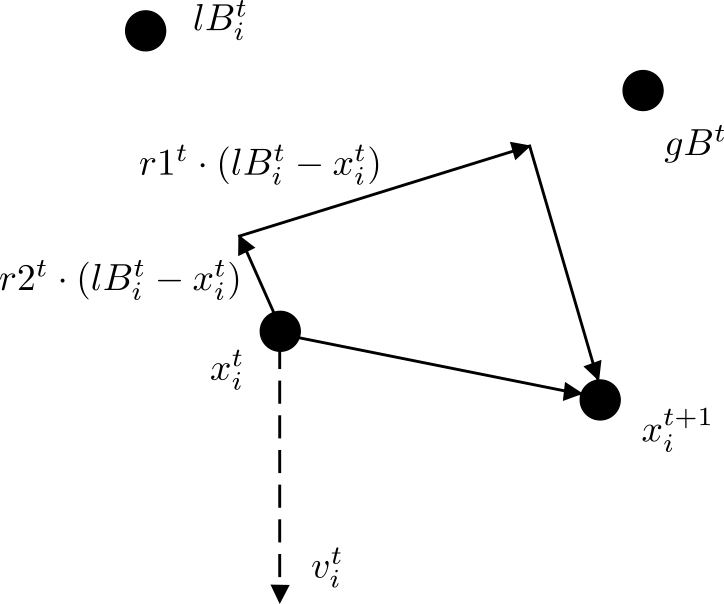
\includegraphics[scale=0.4]{"Part 2 - Search-Based Optimization/Particle Swarm Optimization/Images/Fig.1.3.png"}
\caption{Velocity and movement of particles in PSO.}
\label{fig:PSOmovement}
\end{figure}

\subsection{A PSO example}

To show how the PSO works here is presented a graphical example. Figure~\ref{fig:f1} shows the peaks function plotted in 3D with a lateral view. This function is commonly used in the literature to explain the behavior of optimization algorithms. Figure~\ref{fig:f2} shows the random initialization of the population of a particle (swarm) in PSO \cite{kennedy1995particle}. The population has 30 particles uniformly distributed in the search space defined by the peaks function with an upper bound as $ub=3$ and a lower bound as $lb=-3$ (from the top view).\\
The examples show the distribution of particles at different stages of the optimization process establishing $1000$ iterations as a stop criteria. In Figs.~\ref{fig:f3}, \ref{fig:f4}, \ref{fig:f5} and \ref{fig:f6} it is shown the interaction of the swarm in 50, 300, 600 and 999 iterations in the test function. Finally, in Fig.~\ref{fig:f6} it is possible to see that the swarm has found the zone of the global minimum according to the color bar for the z-axis of Fig.~\ref{fig:f1}.

\begin{figure}[hbp]
  \begin{subfigure}[b]{0.5\textwidth}
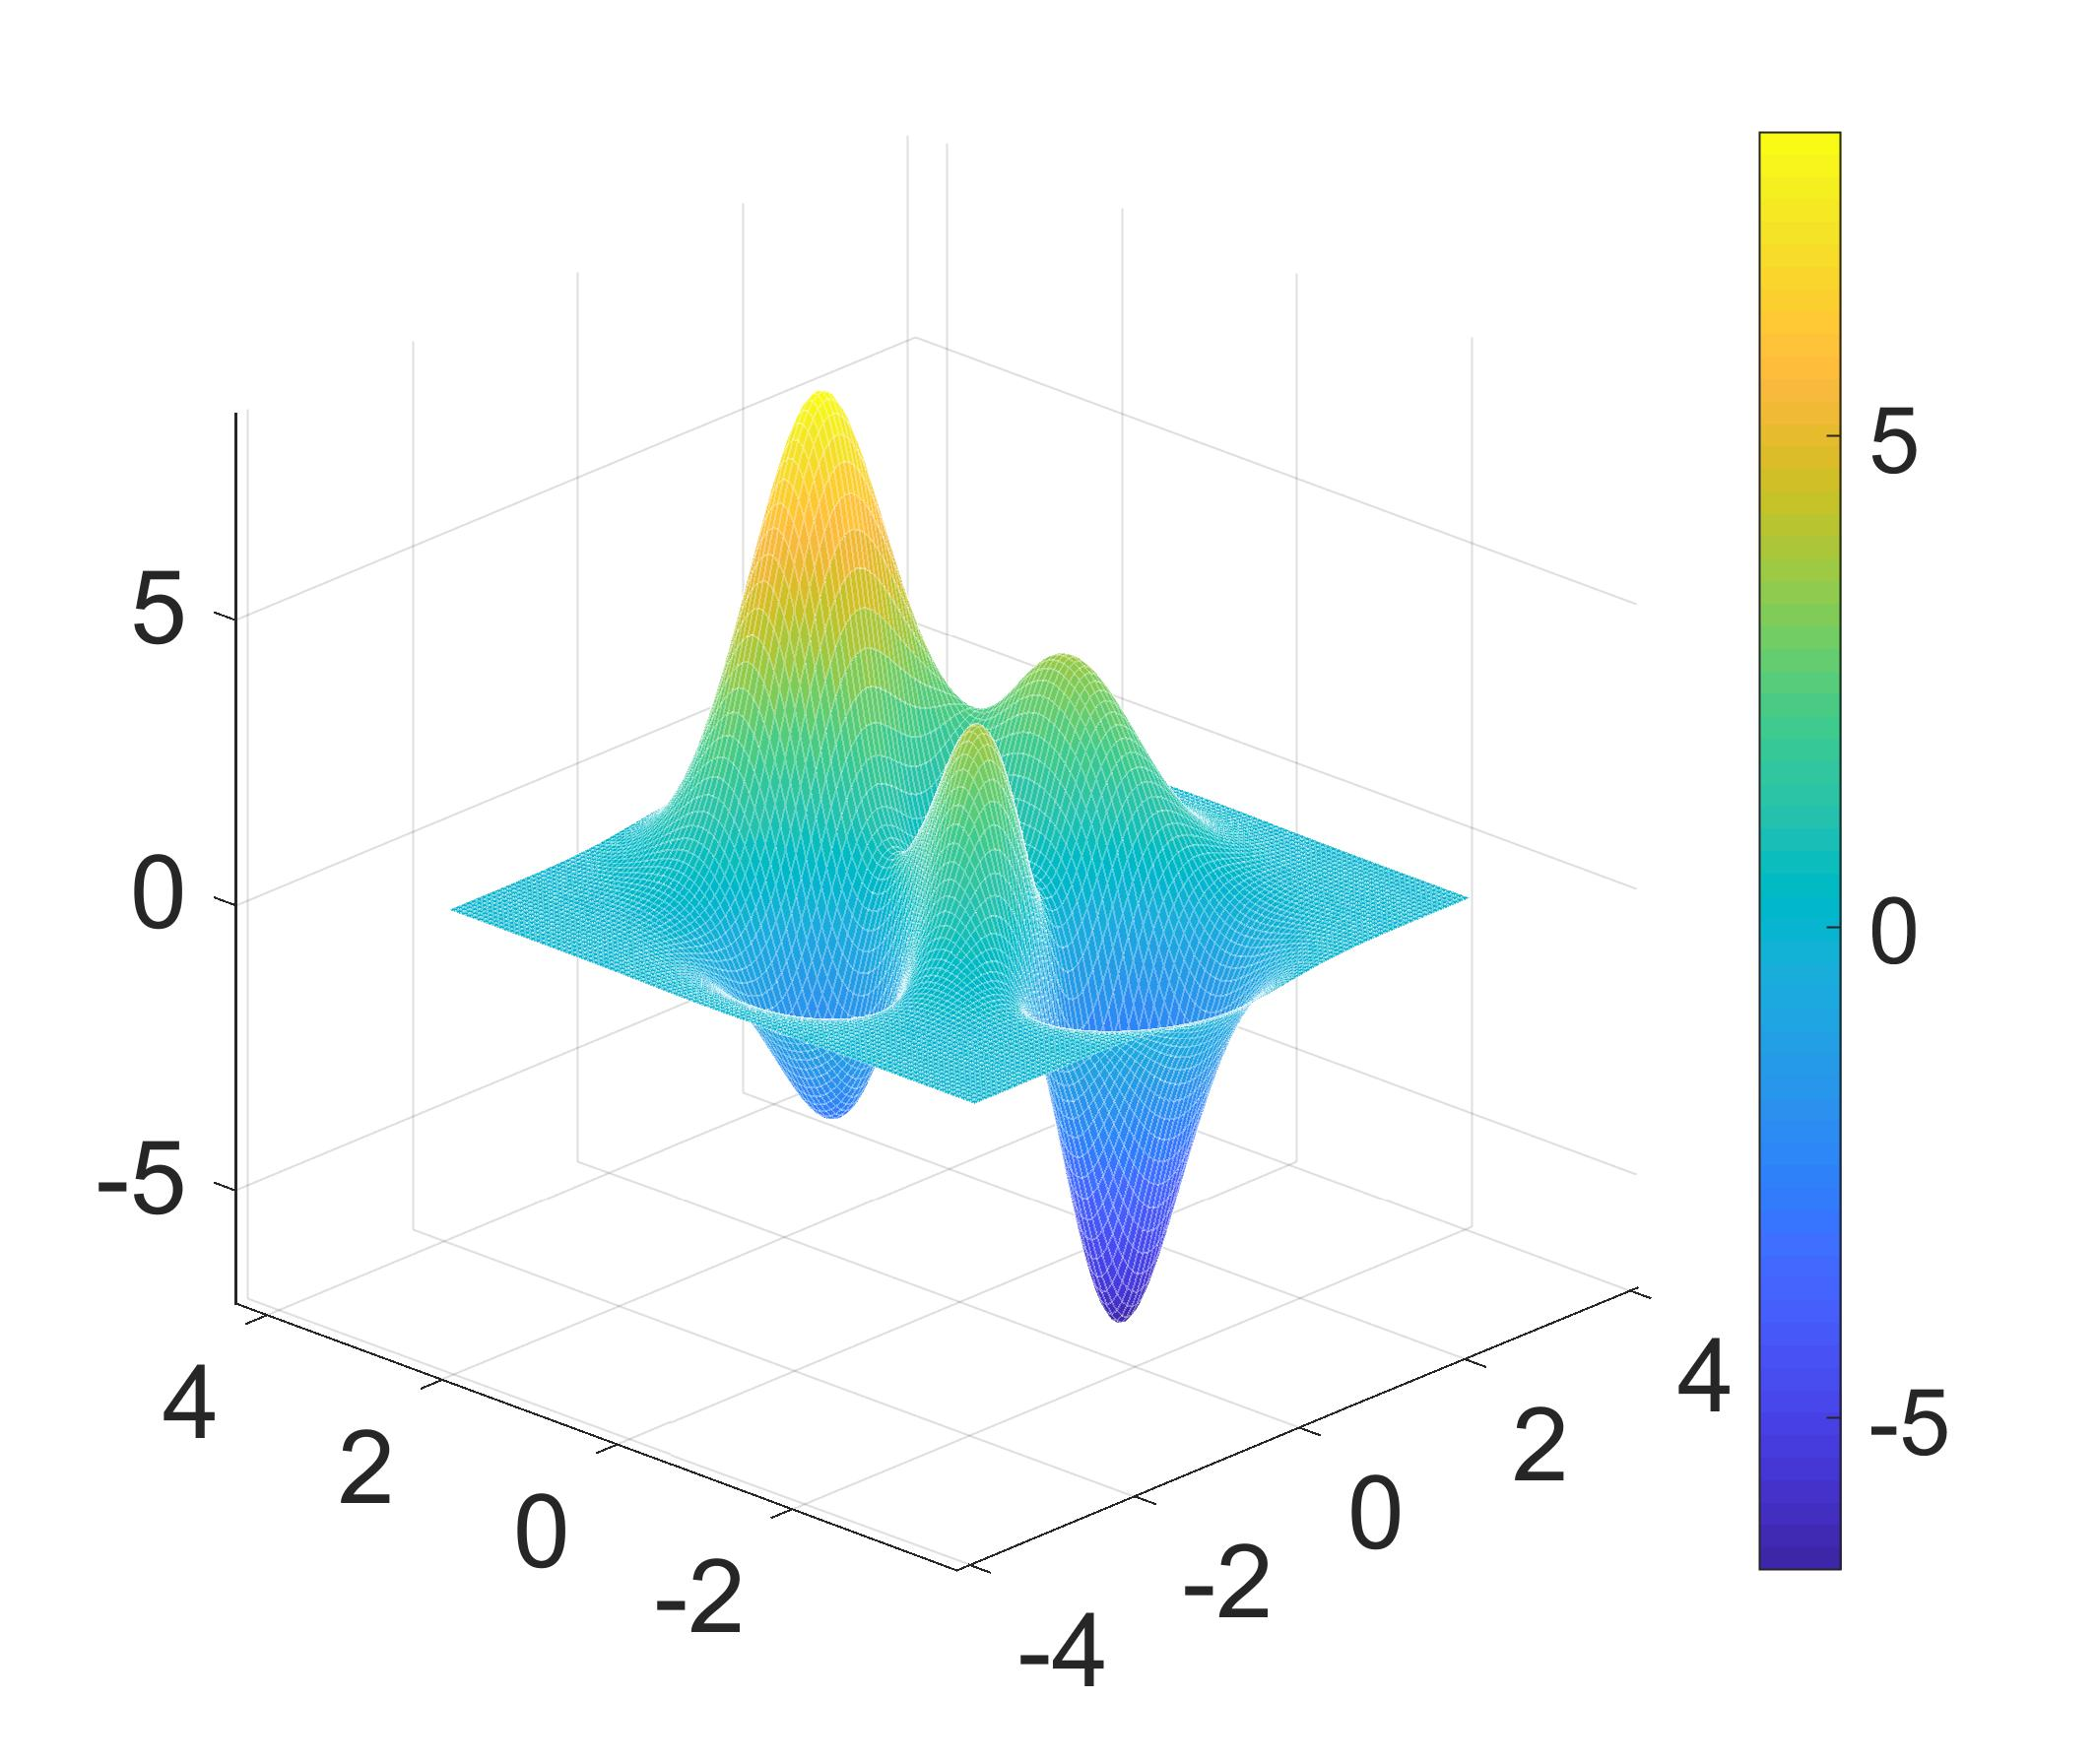
\includegraphics[width=\textwidth, height=\textwidth]{"Part 2 - Search-Based Optimization/Particle Swarm Optimization/Images/FIG1.1.jpg"}
    \caption{Peaks function.}
    \label{fig:f1}
  \end{subfigure}
  \hfill
  \begin{subfigure}[b]{0.5\textwidth}
    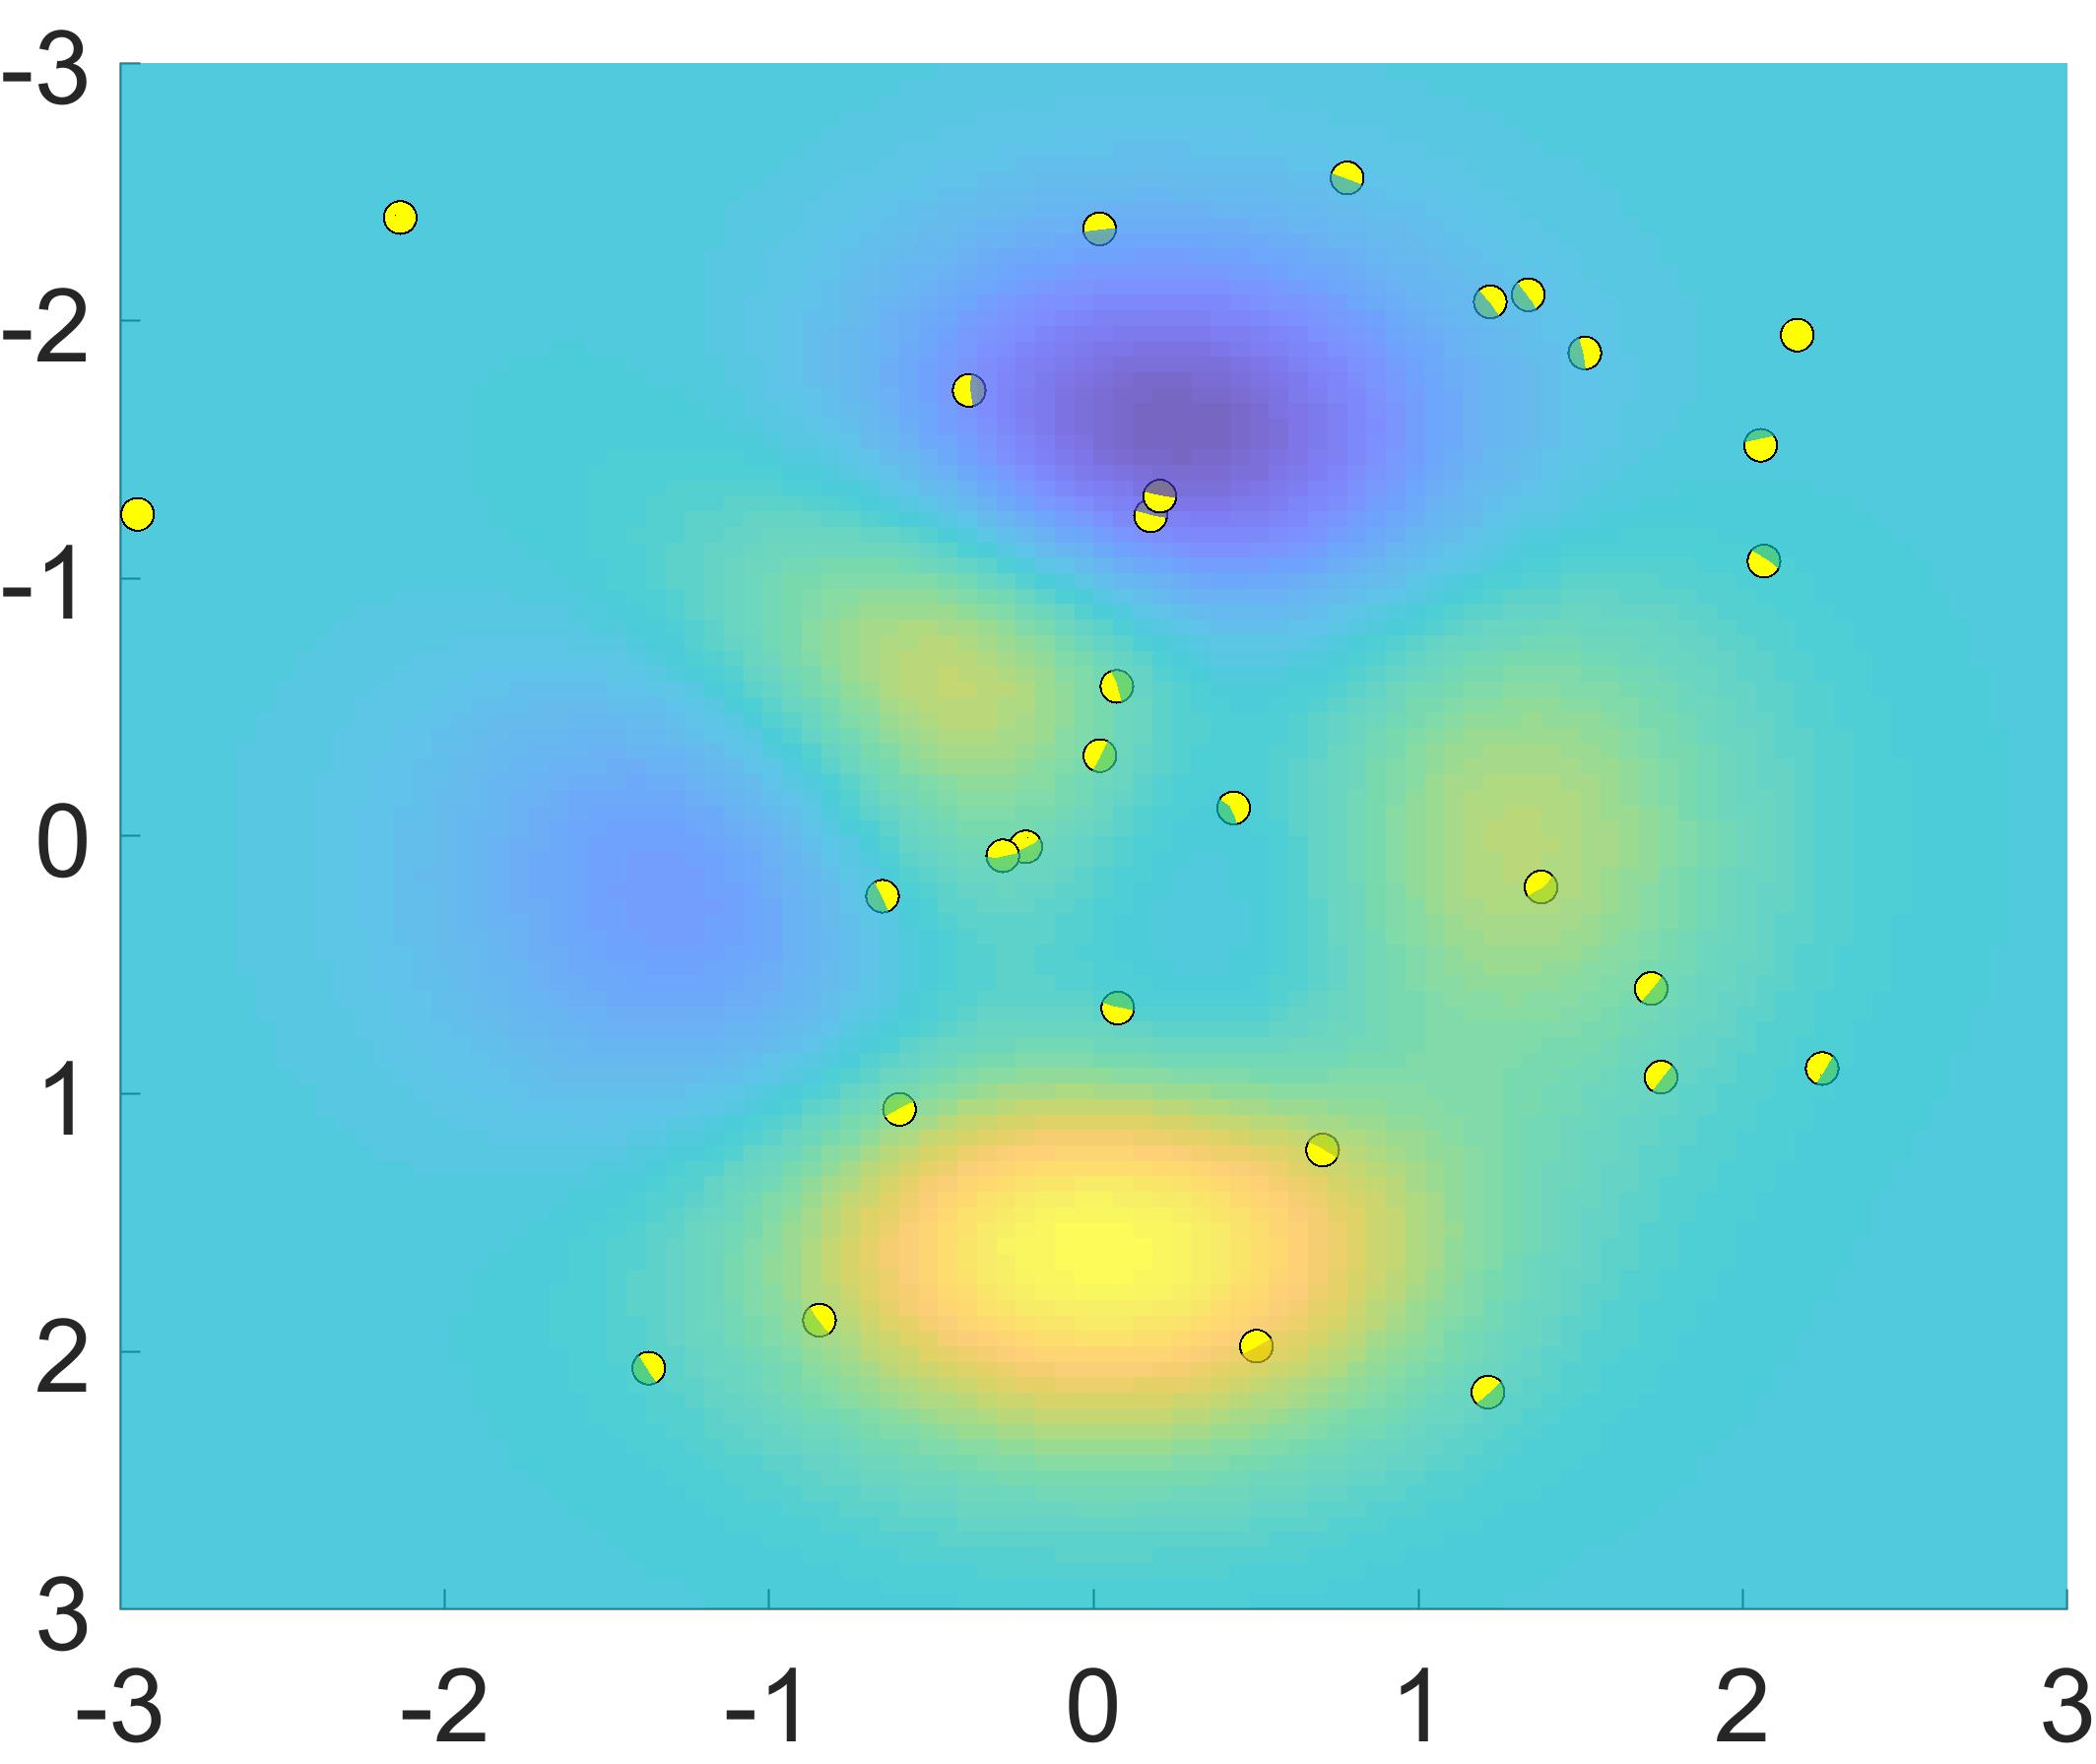
\includegraphics[width=\textwidth, height=\textwidth]{"Part 2 - Search-Based Optimization/Particle Swarm Optimization/Images/FIG2.1.jpg"}
    \caption{Distribution of the swarm at the initialization.}
    \label{fig:f2}
  \end{subfigure}
  \begin{subfigure}[b]{0.5\textwidth}
    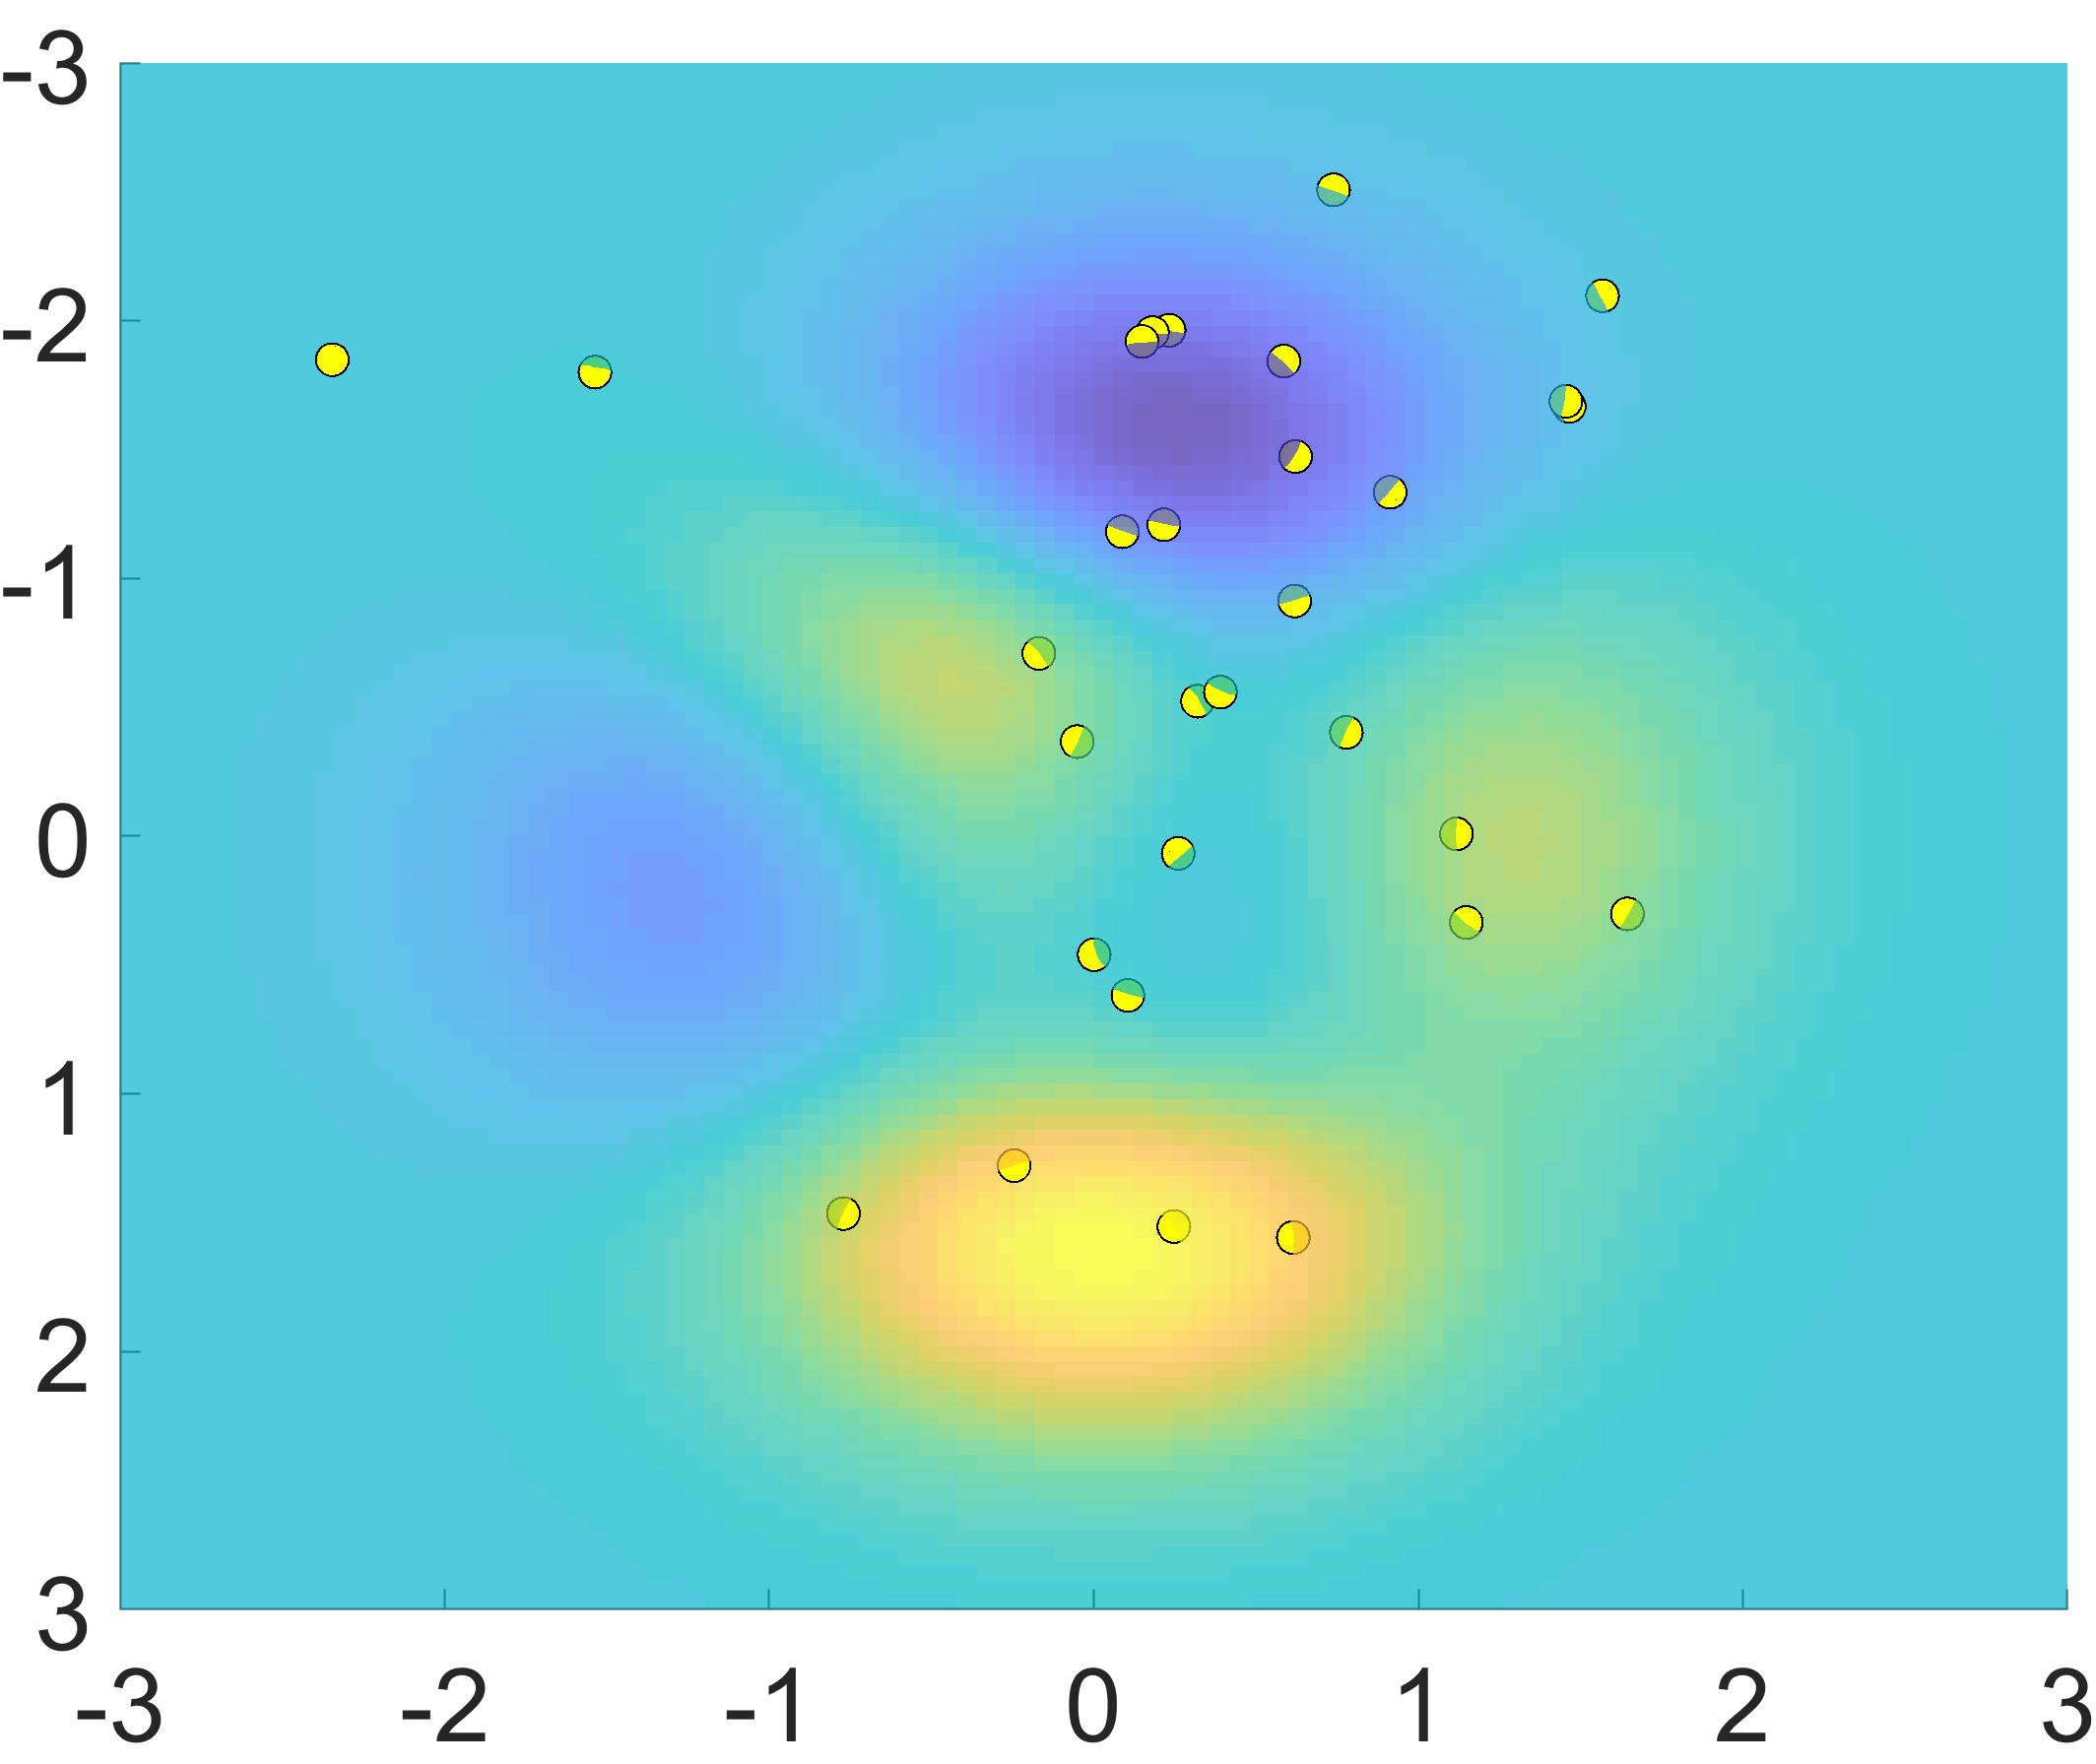
\includegraphics[width=\textwidth, height=\textwidth]{"Part 2 - Search-Based Optimization/Particle Swarm Optimization/Images/FIG3.1.jpg"}
    \caption{Distribution of the swarm at 50 iterations.}
    \label{fig:f3}
  \end{subfigure}
  \begin{subfigure}[b]{0.5\textwidth}
    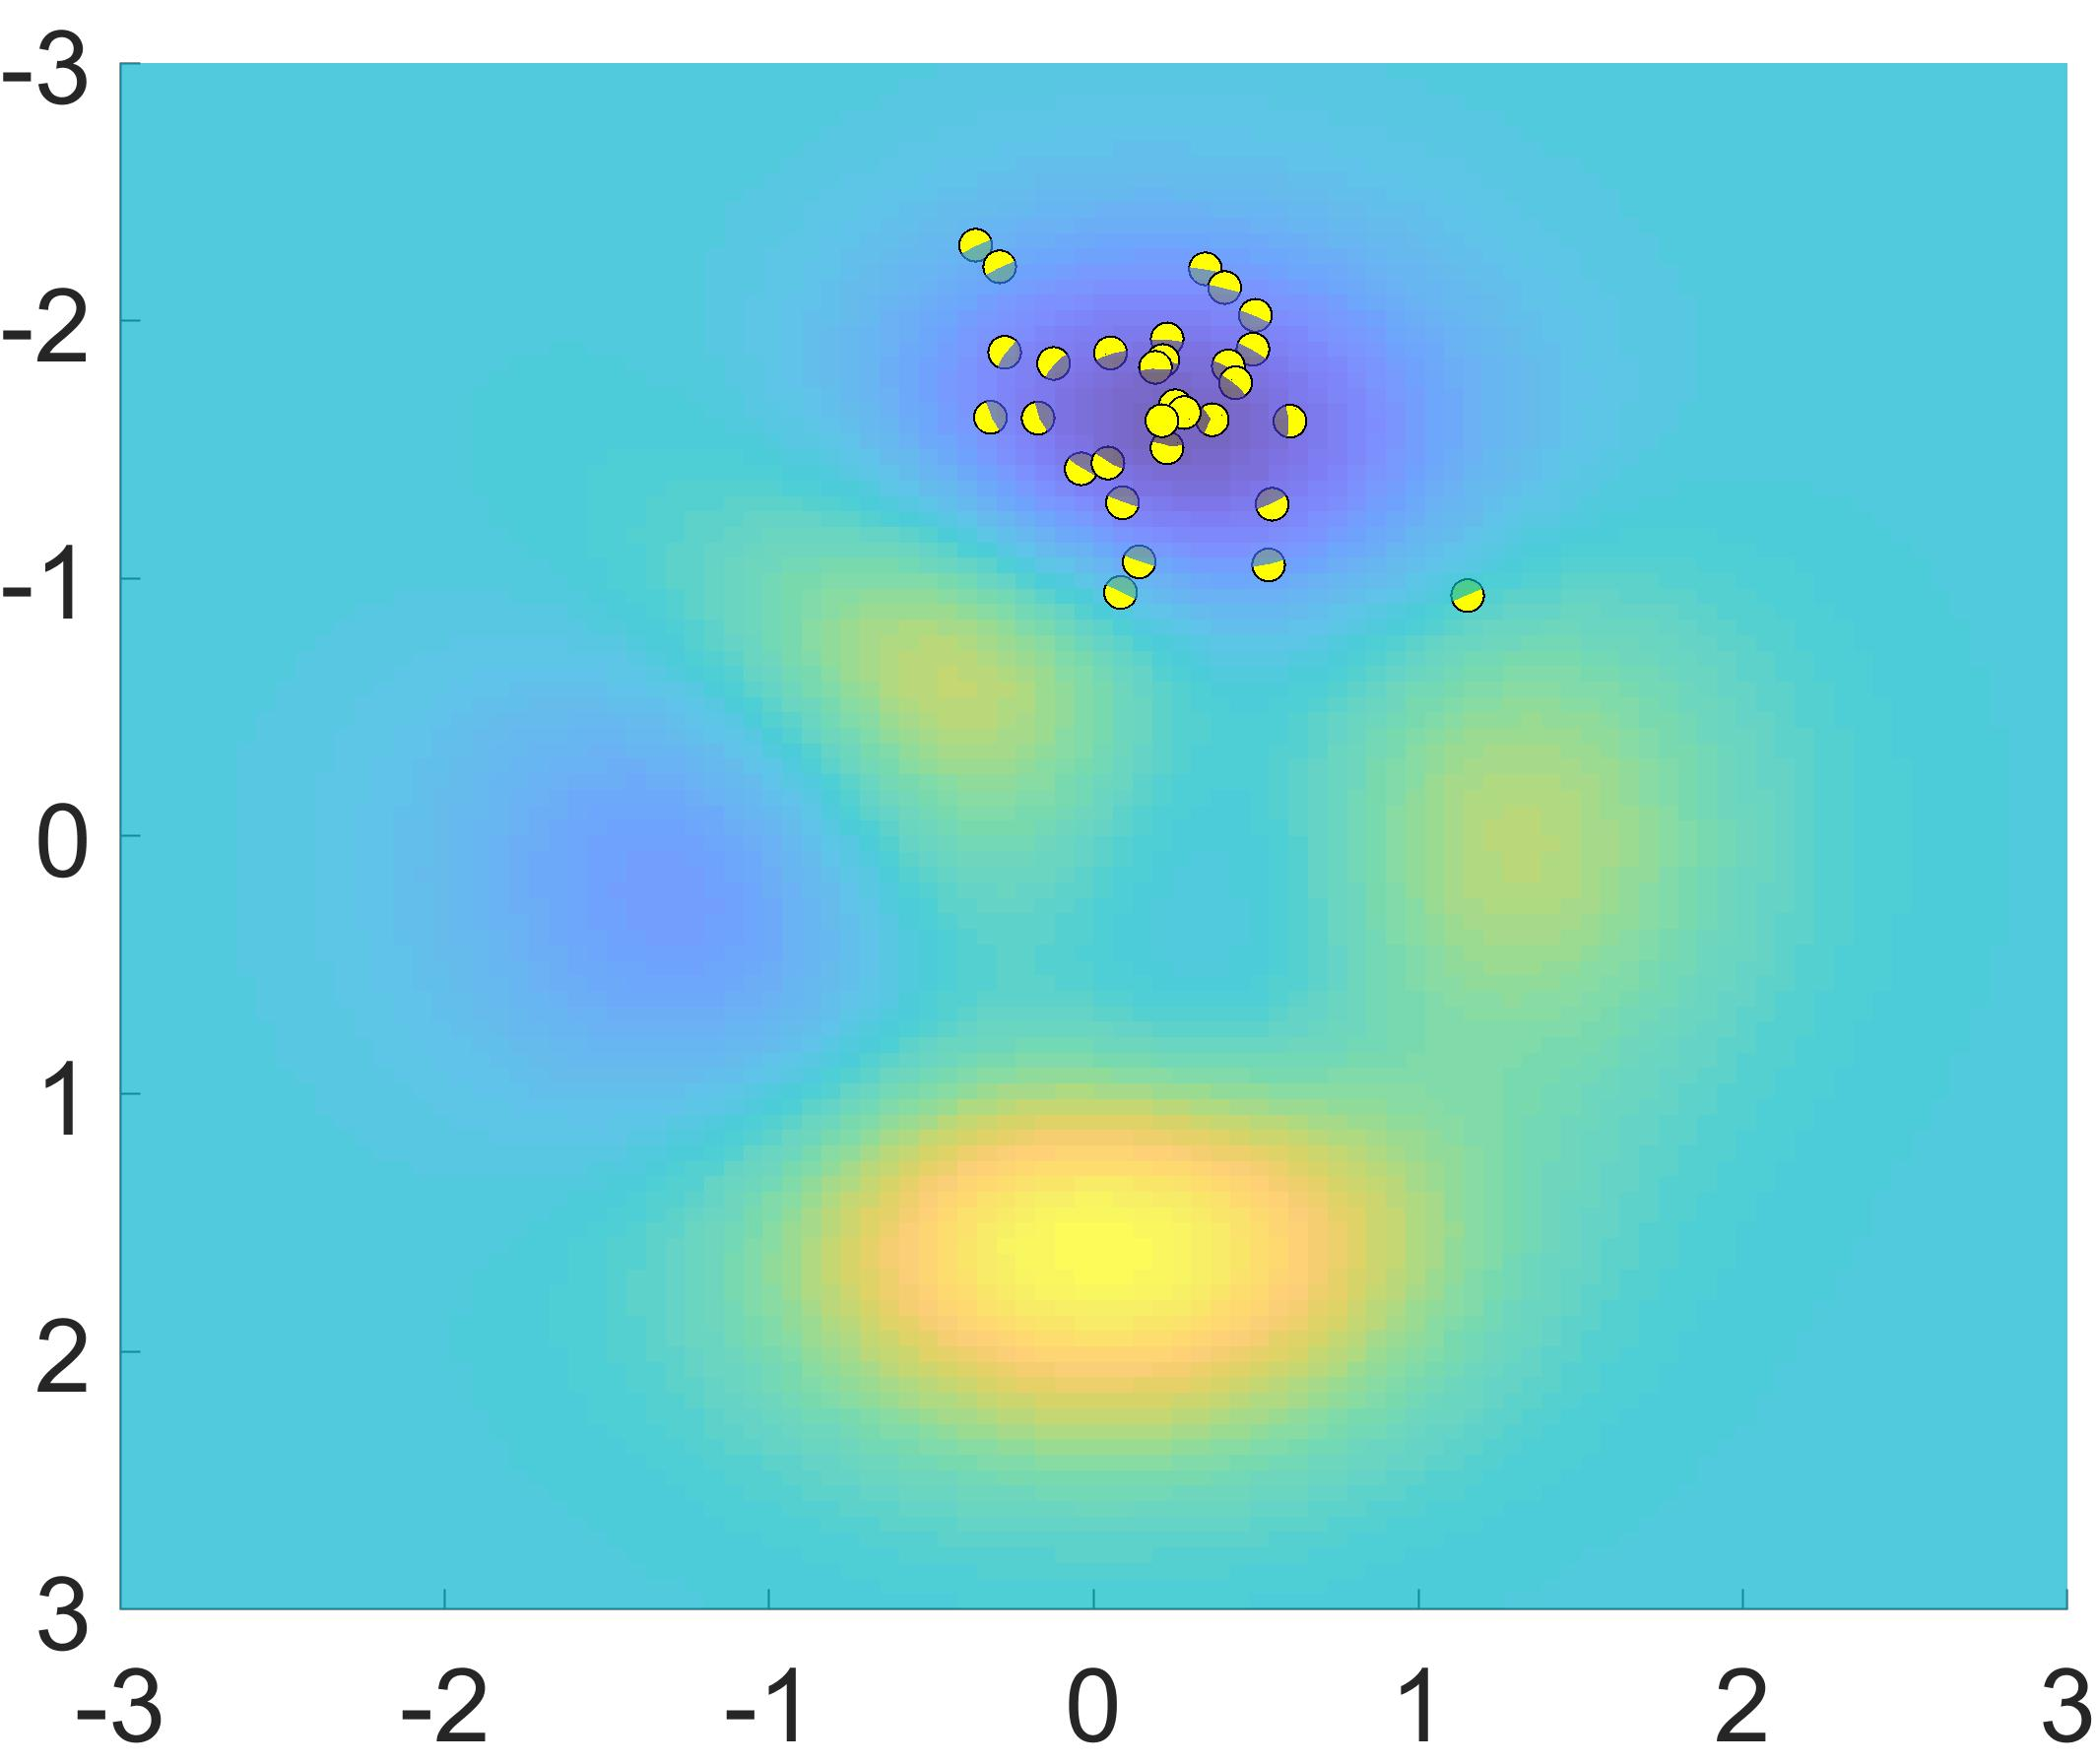
\includegraphics[width=\textwidth, height=\textwidth]{"Part 2 - Search-Based Optimization/Particle Swarm Optimization/Images/FIG4.1.jpg"}
    \caption{Distribution of the swarm at 300 iterations.}
    \label{fig:f4}
  \end{subfigure}
  \begin{subfigure}[b]{0.5\textwidth}
    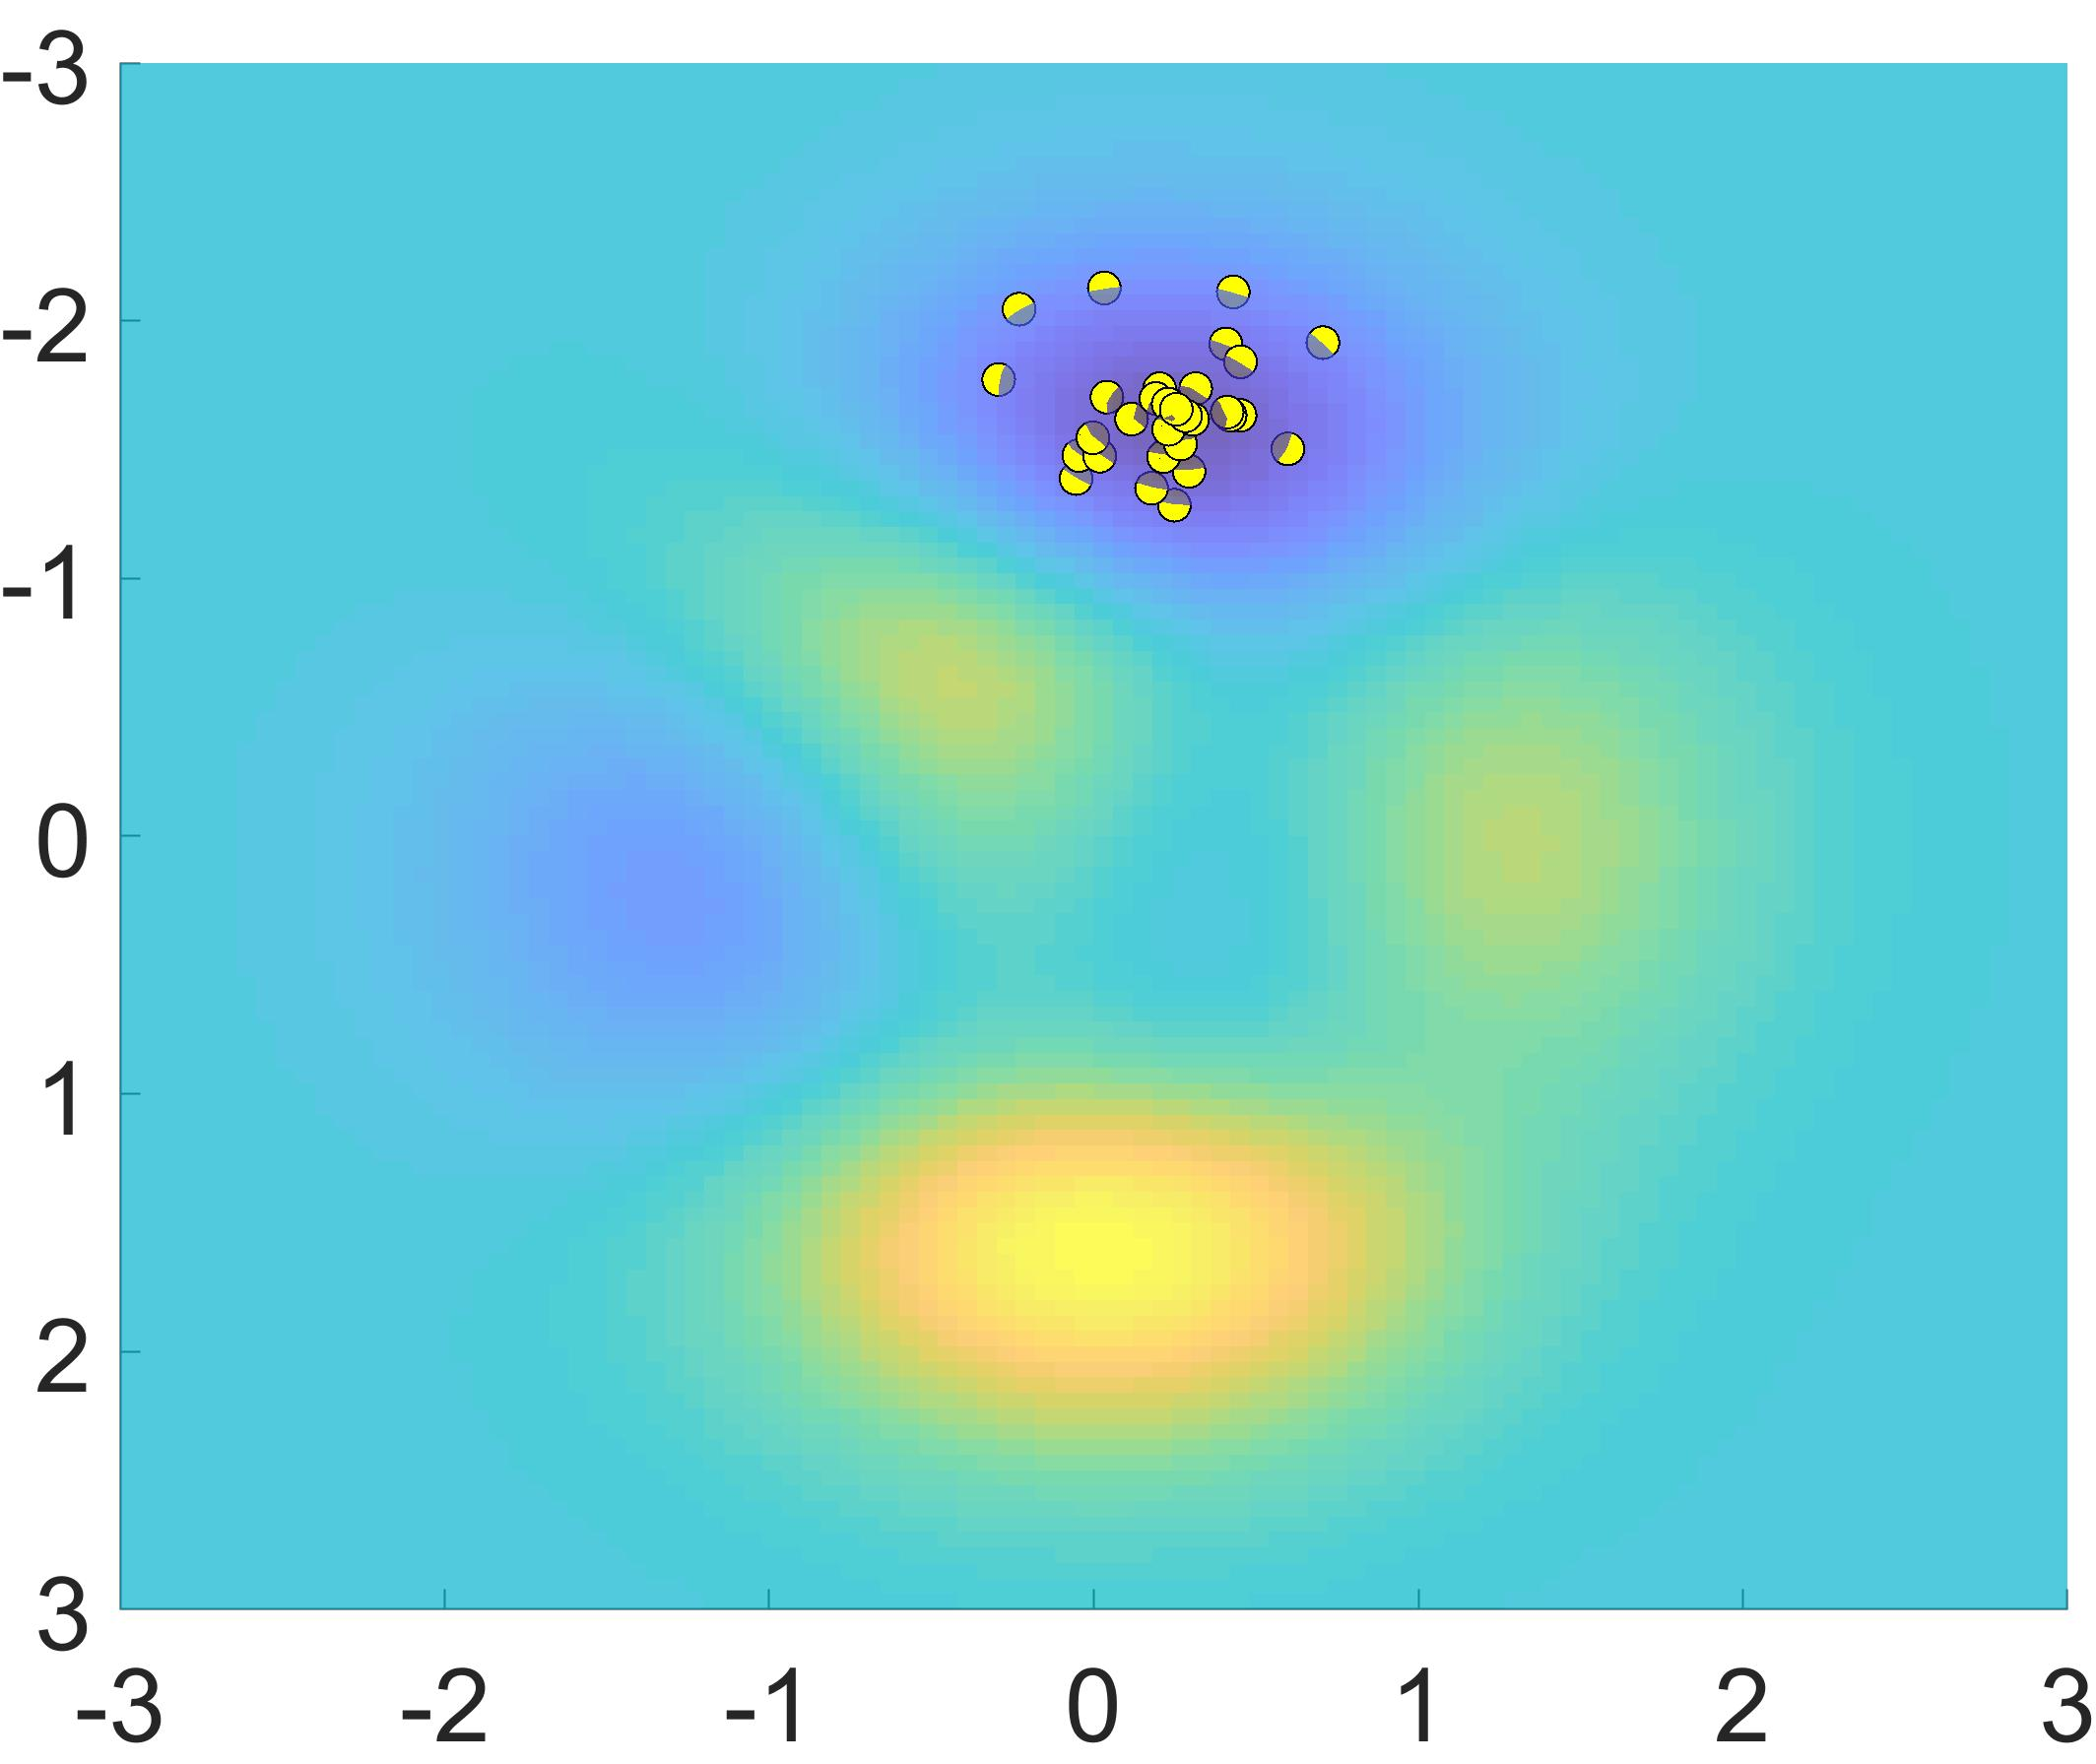
\includegraphics[width=\textwidth, height=\textwidth]{"Part 2 - Search-Based Optimization/Particle Swarm Optimization/Images/FIG5.1.jpg"}
    \caption{Distribution of the swarm at 600 iterations.}
    \label{fig:f5}
  \end{subfigure}
   \begin{subfigure}[b]{0.5\textwidth}
    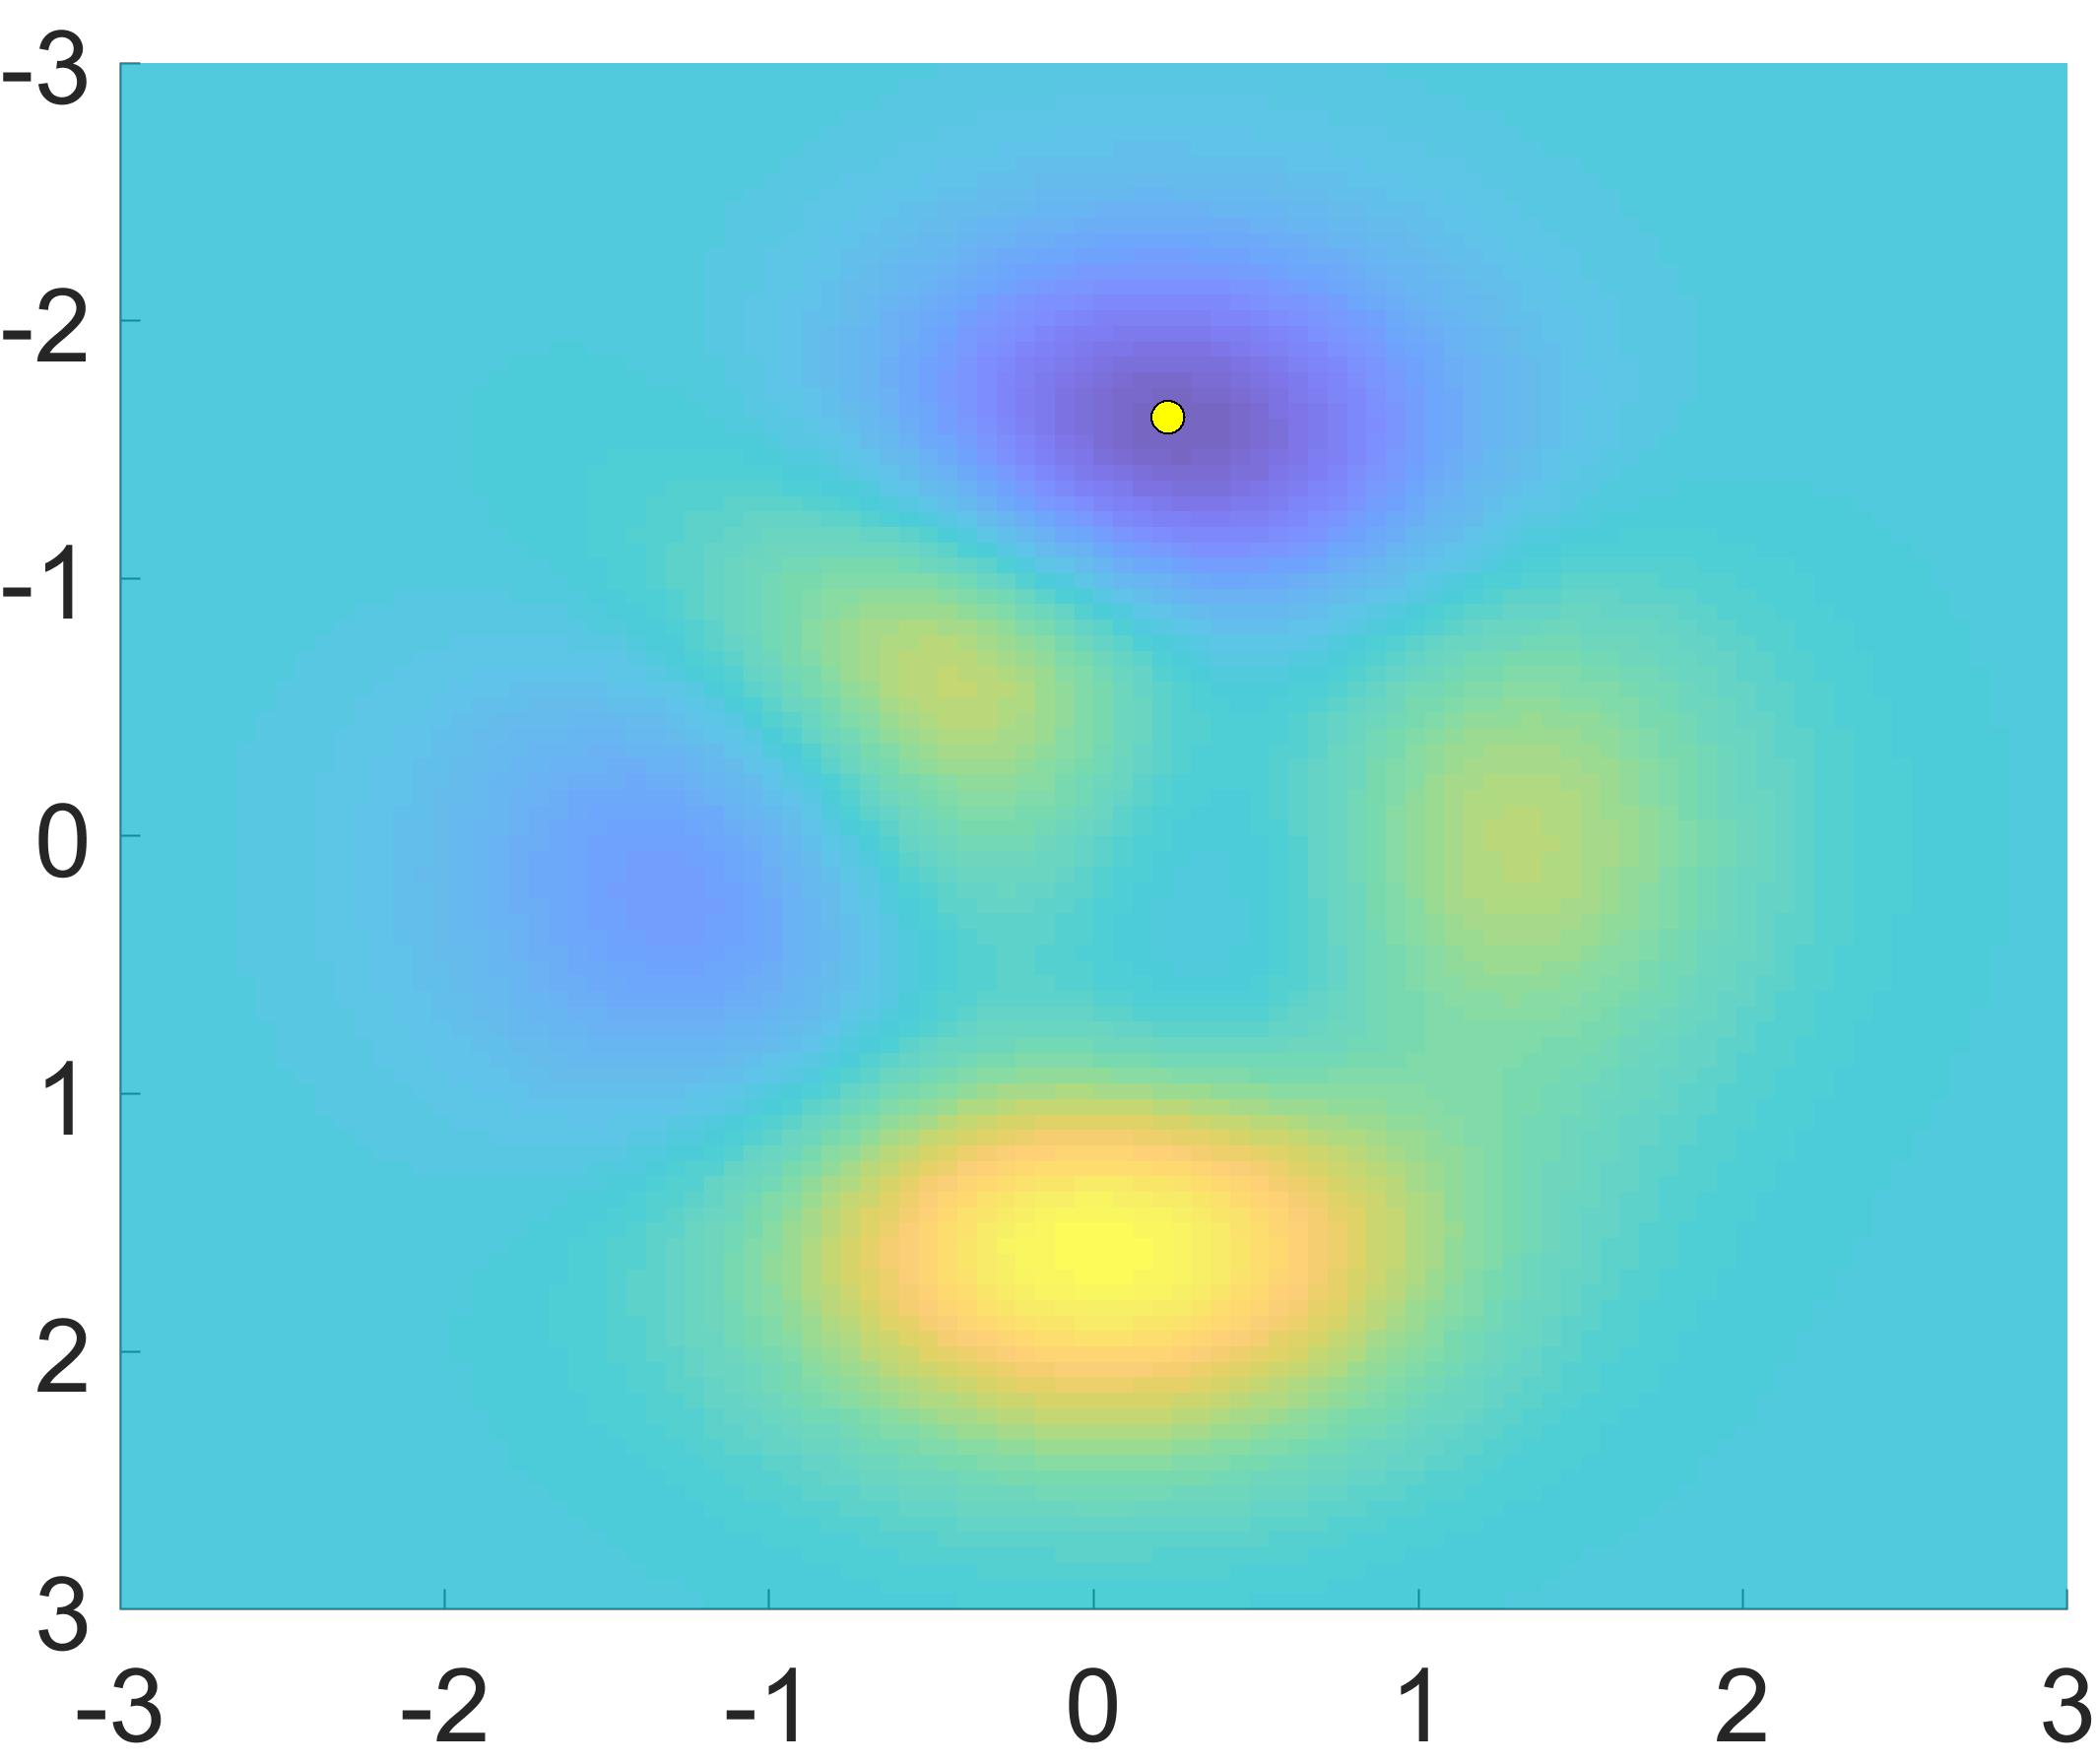
\includegraphics[width=\textwidth, height=\textwidth]{"Part 2 - Search-Based Optimization/Particle Swarm Optimization/Images/FIG8.1.jpg"}
    \caption{Final distribution of the swarm at 999 iterations.}
    \label{fig:f6}
  \end{subfigure}
  \caption{An example of the PSO along the iterative process.}
  \label{fig:fplots}
\end{figure}

%Optimization problems are problems where we want to find solutions that minimize or maximize one or more objective functions, potentially subject to certain constraints. Some examples are:

%\begin{itemize}
%\item Routing problems, e.g., to find a path from a city of origin to a city of destination that minimizes the distance travelled, while ensuring that non-existent direct paths between any two cities are not used. 
%\item Bin packing problems, e.g., to find an assignment of items to bins that minimizes the number of bins used, while ensuring that the maximum volume of the bins is not exceeded.
%\item Scheduling problems, e.g., to find an allocation of staff to tasks in a software project, so as to minimize the cost and duration of this project, while ensuring that staff are only allocated to tasks for which they have the necessary skills.
%\item Hyperparameter optimization, e.g., to find the hyperparameter values that minimize the loss (error) on the validation set for a given machine learning algorithm.
%\end{itemize}

%As we can see, in all examples above, we are interested in minimizing or maximizing a certain function (e.g., the distance travelled, the number of bins used, the cost and duration of the project and the error on the validation set). And, several these problems specify certain constraints (e.g., ensuring that non-existent direct paths are not used, ensuring that the maximum volume of the bins is not exceeded, and ensuring that staff have the necessary skills). Candidate solutions to optimization problems are referred to as \textit{feasible} if they satisfy the constraints of the problem, and \textit{infeasible} when they fail to satisfy one or more constraints.

%The examples above have been mentioned in rough terms, to give a general idea of what optimization problems are. In Section \ref{sec:formulation}, we will see what needs to be specified to formulate them more formally, so that they can be solved by optimization algorithms.


%\subsection{Optimization Algorithms}

%Optimization algorithms are algorithms that attempt to find solutions to optimization problems. They typically create one (or more) full initial candidate solutions to the problem, and then try to iteratively improve such candidate solution(s) in an attempt to find an optimal solution. This is different from search tree-based search algorithms, which attempt to systematically explore the search space to find actions that build a solution over time. 

%For example, consider a routing problem where we wish to find a path to go from a given city A to city F. Consider also that cities B, C, D, E, G, H are also cities in the map. A search tree-based algorithm would start with city A, and then it may add city B to this path, and then add city C, and so on, until a full path between city A and city F is found. Such path is being constructed over time by systematically exploring the space of possible paths in the problem.

%Different from that, an optimization algorithm to solve a routing problem might start with an initial solution which consists of a vector of cities [A, B, C, G]. The algorithm would consider this to be a full \textit{candidate} solution to the problem, despite being infeasible, as it does not reach the destination city F. The algorithm would then modify this candidate solution over time, possibly by replacing, adding or removing cities, in an attempt to find better candidates solutions to the problem. 

%Optimization algorithms typically do not maintain a data structure to store all the explored portion of the space of possible solutions to the problem, being usually more space-efficient than search tree-based algorithms. Several optimization algorithms from the artificial intelligence literature are also more time efficient than the search tree-based algorithms, depending on the problem that is being solved. In addition, they usually don't require problem-specific heuristics that are difficult to design, which is an advantage over search algorithms such as A*. Optimization algorithms from the artificial intelligence literature are frequently \textit{not guaranteed} to find optimal or feasible solutions, but will frequently be able to find good (or near optimal) solutions in a reasonable amount of time.


%\subsection{Formulating Optimization Problems}
%\label{sec:formulation}

%Without loss of generality, an optimization problem is a problem with the following general form:
%\[
%\begin{tabular}{ll}
%minimize        & $f_k(\mathbf{x})$, \ \ \ \ \ \ \ \ \ \ \ $k=\{1,2,\cdots,p\}$ \\ 
%subject to      & $g_i(\mathbf{x}) \leq 0$, \ \ \ \ \ $i=\{1,2,\cdots,m\}$ \\
%                & $h_j(\mathbf{x}) = 0$, \ \ \ \ \ $j=\{1,2,\cdots,n\}$ \\
%\end{tabular}
%\]

%Here, we wish to find a solution $\mathbf{x} \in \mathcal{X}$ that minimizes the functions $f_k(\mathbf{x})$ while satisfying the constraints $g_i(\mathbf{x}) \leq 0$ and $h_i(\mathbf{x}) = 0$, where $p$ is the number of objective functions to be optimised, $m$ is the number of constraints of the type $g_i$ and $n$ is the number of constraints of the type $h_j$ and $\mathcal{X}$ is the domain of $\mathbf{x}$. 

%Such kind of problem contains three main components:
%\begin{itemize}
%\item \textit{Design variable} $\mathbf{x}$. This is the variable that represents candidate solutions to the optimization problem. The domain $\mathcal{X}$ of $\mathbf{x}$ depends on the optimization problem, and could consist of numeric, categorical or ordinal variables, a mix of these, or any other kind of variable that may be relevant to the problem. In addition, $\mathbf{x}$ is not necessarily a vector. It could be any other kind of data structure that may be relevant to the problem in hands. For example, if one is trying to allocate staff members to tasks in a problem, it would be reasonable to consider that $\mathbf{x}$ is a matrix where the rows represent staff members and the columns represent tasks, where each position $x_{i,j}$ contains the value 1 if staff member $i$ is allocated to task $j$ and 0 otherwise. The design variable and its domain define the \textit{search space} of the optimization problem. This is the space of all possible candidate solutions to the problem.

%\item \textit{Objective function(s)} $f_k(\mathbf{x})$, where $k=\{1,2,\cdots,p\}$. These are the functions that we wish to optimise (maximize or minimize). We refer to a problem where $p=1$ as a single-objective optimization problem, and to a problem where $p>1$ as a multi-objective optimization problem. When dealing with a single-objective optimization problem, the $k$ value is frequently omitted from the name of the objective function, i.e., we typically write $f(\mathbf{x})$ instead of $f_1(\mathbf{x})$. You may also hear the term many-objective optimization problems when there are $p>3$ objectives. You will note that the general form above lists a minimisation problem. We can also replace ``minimize'' by ``maximize'' in the general form above if we are dealing with a maximisation problem. It is also possible to use a mix of objectives to be minimized and maximized. However, it is possible to convert maximisation problems into minimisation problems, reason why the general form above lists only minimisation without loss of generality. 

%\item \textit{Constraint(s)}  $g_i(\mathbf{x}) \leq 0$ and $h_j(\mathbf{x}) = 0$, where $i=\{1,2,\cdots,m\}$ and $j=\{1,2,\cdots,n\}$. These are the constraints that a candidate solution $\mathbf{x}$ must satisfy in order to be a feasible solution to the problem. The $g_i$ type of constraints are called inequality constraints, whereas the $h_j$ type of constraints are called the equality constraints. When $m=0$ and $n=0$, the problem is called an unconstrained optimization problem. When $m>0$ or $n>0$, the problem is called a constrained optimization problem. Problems may also involve constraints with inequalities of the type $\geq$ instead of $\leq$. However, it is possible to convert inequalities of the type $\geq$ to inequalities of the type $\leq$, reason why the general form above lists only $\leq$ without loss of generality \footnote{Strict inequalities ($>$ or $<$) are typically not used in optimization problems, as they can lead to ill-posed problems. For instance, consider a problem where we wish to minimize $f(x) = x^2$, subject to $x>0$, where $x$ is a real value. Had the constraint been $x \geq 0$, the optimal solution would have been $x=0$. However, as the constraint is $x>0$, there is no minimizing value. You can always get $x$ values that are closer and closer and close to zero, without ever reaching a minimum. Alternatively, if $x$ was an integer value, this problem would not occur. However, in this case it would be possible to convert the strict inequality $x>0$ into the inequality $x\geq 1$, meaning that the general form of the optimization problem does not need to have strict inequality constraints.}.
%\end{itemize}

%In order to formulate an optimization problem, all the components above must be specified. The more mathematical the problem formulation is, the less ambiguous it is likely to be. However, more mathematical formulations may become more abstract, meaning that it may become more difficult to understand its underlying meaning in the context of the problem of interest. Therefore, it is advisable to provide a problem formulation that is the most formal (mathematical) possible, while including an explanation of it using natural language. %Some examples of problem formulations are provided in the lecture slides.

%\section{Dealing with Constraints}
%
%Optimization algorithms from the artificial intelligence literature frequently don't include themselves strategies to deal with constraints. Instead, we need to design such strategies. There are many different ways to deal with constraints in optimization algorithms. Two examples of strategies are the following:
%
%\begin{itemize}
%\item Representation, initialisation and neighbourhood operators: this kind of strategy requires to design a representation, initialisation procedure and neighbourhood operators that do not allow any infeasible solution to ever be generated by the optimization algorithm. Its advantage is that it makes the optimization algorithms complete, i.e., guaranteed to find feasible solutions. Its disadvantage is that it is problem-dependent and thus not easy to design. Moreover, it may restrict the search space too much, which can sometimes hinder the search for optimal solutions. In the worse case scenario, such restrictions may eliminate the optimal solution from the reachable areas of the search space, meaning that the optimal solution cannot be found. 
%
%Some optimization algorithms are not based on neighbourhood operators, but other kinds of operators. In such cases, these other kinds of operators must also ensure that infeasible solutions are never generated.
%
%\item Objective function: it is possible to modify the objective function in order to penalise the objective values of infeasible solutions. Considering the general form of optimization problems shown in Section \ref{sec:formulation} with $k=1$, the objective function could be modified as shown below in order to deal with the constraints.
%
%\[
%\begin{tabular}{ll}
%minimize        & $f(\mathbf{x}) + Q(\mathbf{x})$\\
%subject to      & $g_i(\mathbf{x}) \leq 0$, \ \ \ \ \ $i=\{1,2,\cdots,m\}$ \\
%                & $h_j(\mathbf{x}) = 0$, \ \ \ \ \ $j=\{1,2,\cdots,n\}$ \\
%\end{tabular}
%\]
%
%\noindent where:
%
%\[ Q(\mathbf{x}) =
%  \begin{cases}
%    0       & \text{if } \mathbf{x} \text{ is feasible.}\\
%    P [g_a(\mathbf{x})^2 + g_b(\mathbf{x})^2 + \cdots + h_{a'}(\mathbf{x})^2 + h_{b'}(\mathbf{x})^2 + \cdots] & \text{otherwise}
%  \end{cases}
%\]
%
%\noindent where $P$ is a very large positive constant, and the indexes $a$, $b$, ..., $a'$, $b'$, ..., represent the indexes of the constraints that are violated. For example, consider a candidate solution $\mathbf{x}$ that violates only the constraints $g_2(\mathbf{x})$, $g_5(\mathbf{x})$ and $h_3(\mathbf{x})$. In this case, $Q(\mathbf{x}) = P [g_2(\mathbf{x})^2 + g_5(\mathbf{x})^2 + h_3(\mathbf{x})^2]$. The constant $P$ should ideally be large enough to make the objective value of infeasible solutions worse (larger) than the objective value of any feasible solution. The power of two used in the functions $g$ and $h$ ensures that the values of these functions will always be positive, such that the penalty will always increase (worsen) the objective value. % \footnote{The use of square can also help the optimization process depending on the optimization algorithm being adopted. This is because it causes the values of the objective function of infeasible solutions that violate a given constraint by different amounts to differ more from each other. For example, consider an infeasible solution $\mathbf{x}$ for which $g_a(\mathbf{x}) = 1$ and another infeasible solution $\mathbf{x}$ for which $g_a(\mathbf{x}) = 2$. The penalty applied to these }.
%
%The advantage of this strategy to deal with constraints is that it is very general. The same strategy could potentially be adopted for any optimization problem. However, as it enables infeasible solutions to be generated, the optimization algorithm would have to spend time searching for feasible solutions. For some problems where that are too many infeasible solutions, the algorithm may struggle to find feasible solutions based solely on the objective function, in which case the strategy based on representation, initialisation and neighbourhood operators may be more adequate. 
%
%An example of use of these two types of strategies to deal with constraints is provided in the lecture slides.
%
%
%\end{itemize}

\section{The PSO variants}
\label{sec:variants}

This algorithm has been so successful since its emergence that it has been the base for designing new methods. Same that preserves the essence and structure of the PSO but adds improvements in operators, parameters, initialization, or combines concepts that make the algorithm more specialized for specific problems. The most important variants are listed below, divided into two fields, single-objective and multi-objective optimization:\\ 

\subsection{Top PSO variants for single-objective problems}
\label{tab:pso_variants}
There are many publications related to PSO variants for single-objective optimization. Most of them were compiled and sorted by year of publication, adding the citations obtained from publication date up to the current year $2021$. Based on this information, the top 30 most cited PSO variants were obtained (see Table~\ref{tab:pso_variants}).

\input{"Part 2 - Search-Based Optimization/Particle Swarm Optimization/tables/table1"}


The following is a brief description of the most widely used PSO variants. Considering the ranking in Table~\ref{tab:pso_variants} and some state of the art reviews,~\cite{garcia2012brief},~\cite{sousa2017review}~\cite{sedighizadeh2009particle}~\cite{kameyama2009particle} indicating which are the most popular variants. The objective is to present some of the most representative varieties of the PSO algorithm considering significant modifications in terms of several concepts such as social topology between particles, new definitions of equations for velocity and position, and methodologies that make the algorithm adaptive in some of its global parameters.  

\subsubsection{Standard PSO 2011}

In the initialization process of standard PSO (SPSO), the size of the swarm is defined by the user, but it is empirically suggested $N=40$ particles. The algorithm starts initializing the particles following a random distribution \cite{clerc2010particle}, while the other elements are initialized following a uniform distribution. If any element goes out of bounds, these act as a barrier returning the element within the bounds $[lb_j, up_j]$ resetting the particle velocity to $0$, where $j$ corresponds to the dimension number.
Until the 2007 versions, the velocity is updated dimension by dimension, as can be seen in Eq.~\ref{eq:equation2}, and the performance of the algorithm depends mainly on the coordinate system obtained (rotation sensitivity)~\cite{clerc2012beyond},~\cite{spears2012biases}.


\begin{figure} [H]
\centering
    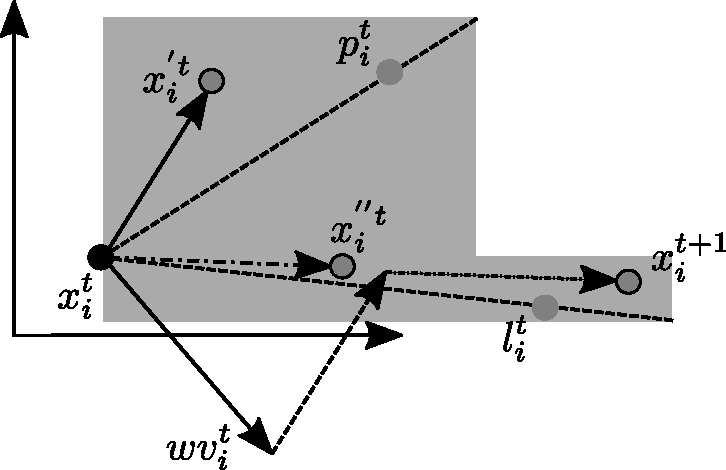
\includegraphics[width=0.60\textwidth]{"Part 2 - Search-Based Optimization/Particle Swarm Optimization/Images/SPSO2011-1.pdf"}
    \caption{Geometrical representation of standard PSO until 2007}
    \label{fig:STANDARDPSO_1}
\end{figure}


    
Figure~\ref{fig:STANDARDPSO_1} shows that each particle at each time step gets its distribution of all nearby positions and which is also a combination of two rectangles $D$ with sides parallel to the axes, with uniform probability distribution within each rectangle. In contrast, the variant proposed in 2011~\cite{clerc2012beyond} suggests the idea of an adaptive random topology in terms of communication between search agents and exploits the idea of rotational invariance (see Fig.~\ref{fig:STANDARDPSO}).


\begin{figure} [H]
\centering
    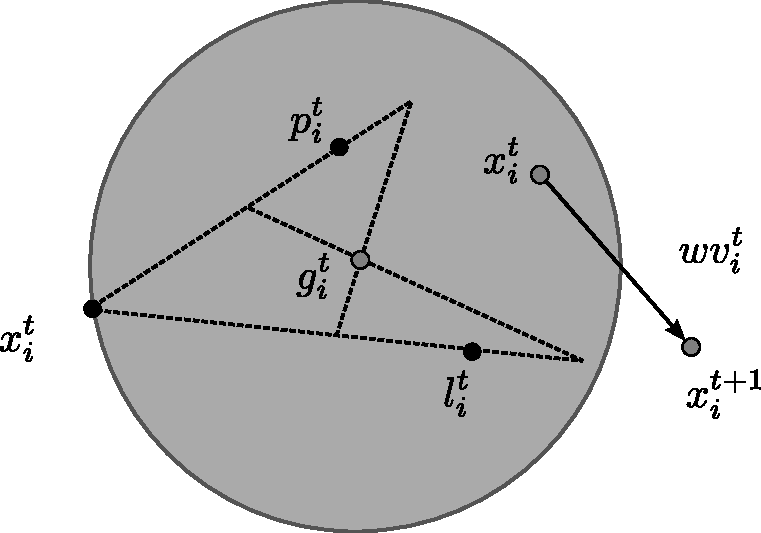
\includegraphics[width=0.60\textwidth]{"Part 2 - Search-Based Optimization/Particle Swarm Optimization/Images/SPSO2011.pdf"}
    \caption{Geometrical representation of standard PSO}
    \label{fig:STANDARDPSO}
\end{figure}



For each particle $i$ and at each time stage $t$, a center of gravity ${\vec{g}}_i^t$ is defined around three points:

\begin{itemize}
    \item The current position~(${\vec{x}}_i^t$)
    \item Point a little ``beyond" the best previous personal position~(${\vec{p}}_i^t$) defined as:
    
    \begin{equation}\label{eq:bestpreviouspersonal position}
        {\vec{p}}_i^t={\vec{x}}_i^t+\ c_1{\vec{r}}1_i^t\otimes(\ {\vec{lB}}_i^t\ - {\vec{x}}_i^t)
    \end{equation}
    
    \item Point a little “beyond” the best previous position in the neighborhood~($ {\vec{l}}_i^t$) defined as:

      \begin{equation}\label{eq:best previous position in the neighbourhood}
        {\vec{l}}_i^t={\vec{x}}_i^t+\ c_2{\vec{r}}2_i^t\otimes(\ {\vec{gB}}^t\ - {\vec{x}}_i^t)
    \end{equation}
    
    \item Center of gravity(${\vec{g}}_i^t$) finally defined as:
    
    \begin{equation}\label{eq:gravitycentre}
        {\vec{g}}_i^t=\frac{\left({\vec{x}}_i^t+{\vec{p}}_i^t+{\vec{l}}_i^t\right)}{3}
    \end{equation}
    
\end{itemize}


In the case of Fig.~\ref{fig:STANDARDPSO} the $distribution~of~all~possible~next~positions$ (DNPP) obtained is a D-dimensional sphere defined as $\mathcal{H}_i({\vec{g}}_i^t, ||\vec{g}_i^t,\vec{x}_i^t||$), which is rotational invariant about its center, i.e., it does not change when the function is rotated.\\
In SPSO-2011, velocity is updated as follows:


\begin{equation}
       {\vec{v}}_i^{t+1}=w{\vec{v}}_i^t{+\mathcal{H}}_i({\vec{g}}_i^t,||\vec{g}_i^t - \vec{x}_i^t||)-\ {\vec{x}}_i^t
\end{equation}


While particle position is updated following Eq.~\eqref{eq:equation3}.

\subsubsection{Fully-informed PSO}

Human social behaviors inspired the authors to conclude that individuals are not influenced by a single individual but by those around them. Based on observations, they proposed a modification of the velocity equation of the canonical version of PSO~\cite{kennedy1995particle} with the purpose that each particle is influenced by the performance of all its neighbors and not by the performance of a single individual. The equations for the update of velocity and position are defined as: 

\begin{equation}\label{eq:speedwithneighbors}
      \vec{v}_i^{t+1}=w\vec{v}_i^t+\sum_{m=1}^{\left|C_i\right|}{\gamma_m^t\frac{(\mathcal{Y}_m^t-x_i^t)}{\left|C_i\right|}}
\end{equation}

\begin{equation}
       \vec{x}_i^{t+1}=\vec{x}_i^t +\ \vec{v}_i^{t+1}
\end{equation}


Inspired by the fact that an individual is influenced by the behavior of the individuals around him, the authors define the Eq.~\ref{eq:speedwithneighbors}. Where $C_i$ is the set of particles in the neighborhood of $i$, and $\gamma_m^t \in [0, c_1+\ c_2]^j$, where $c_1$ and $c_2$ are the learning coefficients, $j$ is the dimensionality of the problem and the position $\mathcal{Y}_m^t$ represents the best position that particle $m$ has visited until iteration $t$ (a position that has obtained the best evaluation of the objective function).
The main contribution of this algorithm published in $2004$ that makes it different from other variants is the type of topology used in its particles~\cite{mendes2004population}. Since they all have the exact source of information, there is no difference in the amount of information shared. Some of the topologies that can affect or improve the performance of PSO are the following:

\begin{itemize}
    \item \textit{Ring}:
      this topology has a network configuration where the particle connections create a circular trajectory. Each particle in the network is fully connected to two others, thus forming a single continuous route, resulting in a ring structure as illustrated in Fig.~\ref{fig:ringtopology}. The algorithm that results from this topology is called Lbest PSO; in addition, such a topology can be generalized to a network structure in which neighborhoods of larger size are used.
    \item \textit{Star}:
    this social topology is shown in Fig.~\ref{fig:startopology}. Here, it is observed that all the particles in the swarm are interconnected. A PSO using the star topology is commonly named the Gbest PSO . The original implementation of the PSO used the star topology~\cite{kennedy1995particle}.
    \item \textit{Von Neumann}:
    this topology is a square grid where each particle has four neighbors. The 2-D variant is represented in Fig.~\ref{fig:squaretopology}, and the 3-D variant is represented in Fig.~\ref{fig:cubetopology}. This class of topologies allows the communication between the particles to be unusual and different from other social communication topologies.
\end{itemize}

\begin{figure}[H]\centering
  \begin{subfigure}[b]{0.23\textwidth}
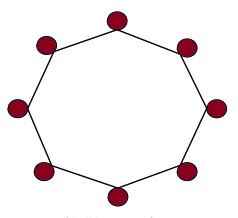
\includegraphics[width=\textwidth]{"Part 2 - Search-Based Optimization/Particle Swarm Optimization/Images/RING.jpg"}
    \caption{Ring.}
    \label{fig:ringtopology}
  \end{subfigure}
 \hfill
  \begin{subfigure}[b]{0.23\textwidth}
    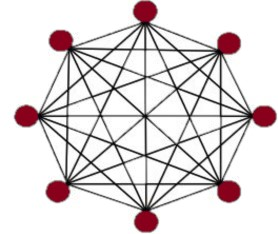
\includegraphics[width=\textwidth]{"Part 2 - Search-Based Optimization/Particle Swarm Optimization/Images/STAR.jpg"}
    \caption{Star.}
    \label{fig:startopology}
  \end{subfigure}
  \hfill
  \begin{subfigure}[b]{0.23\textwidth}
    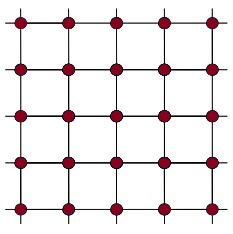
\includegraphics[width=\textwidth]{"Part 2 - Search-Based Optimization/Particle Swarm Optimization/Images/SQUARE.jpg"}
    \caption{Square.}
    \label{fig:squaretopology}
  \end{subfigure}
  \hfill
  \begin{subfigure}[b]{0.23\textwidth}
    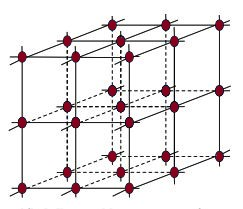
\includegraphics[width=\textwidth]{"Part 2 - Search-Based Optimization/Particle Swarm Optimization/Images/CUBE.jpg"}
    \caption{Cube.}
    \label{fig:cubetopology}
  \end{subfigure}
\caption{Social topologies}
  \label{fig:topologies}
\end{figure}

\subsubsection{Comprehensive Learning PSO}


The main novelty of this algorithm is that the authors propose a new function for updating the particle velocity defined as:

\begin{equation}
     \vec{v}_{i}^{t+1}=w\ast \vec{v}_{i}^t + c \ast {\vec{r1}_i^t} \ast \left ( \vec{lB}_{f_i}^t - \vec{x}_{i}^t \right ) 
\end{equation}


\noindent where $fi=[f_i(1),f_i(2),\cdots,f_i(D)]$ defines which particles of $lB$ the particle $i$ should follow, and $D$ represents the dimensionality of the problem. The value of $lB_{f_i(j),j}$ can be any particle’s $lB$ including its own $lB$. The decision depends on probability $P_c$, referred to as the learning probability, which can take different values for different particles.
For each dimension of particle $i$, the authors generate a random number. If this random number is higher than $P_{c_i}$, the corresponding dimension will learn from its own $lB$; otherwise, it will learn from another particle’s $lB$.The selection method used by the tournament and the main steps for selection are as follows:

\begin{itemize}
    \item First, two particles are chosen randomly from the population, except the particle with its updated velocity.
     \item The objective value of the two particles($lB$) is compared, and the best of these is selected. In CLPSO the objective value is defined as the higher, the better, which means that to solve minimization problems, use the negative values of the function as objective values.
      \item Finally, using the winning particle as an example for the next generations to learn from that dimension, if all individuals are their own $lB$, then a random dimension is chosen for the particles to learn from the best $lB$ particles working on it.
\end{itemize}

\subsubsection{Fuzzy Adaptative PSO} 

This version of PSO is based on fuzzy inference systems. For more information about this computational area, the reader is advised to refer to the following references \cite{Sugeno1985,Jang1993}. Readers may understand this version of PSO more fully after learning about fuzzy inference systems, but a brief description of this approach is provided below.

%\paragraph{\textit{Fuzzy inference system}}
Fuzzy inference systems are basically conditional statements expressed in the form IF A THEN B, where A and B are labels of fuzzy sets defined by appropriate membership functions \cite{Zadeh1973}. A fuzzy inference system is depicted in Fig.~\ref{fig:FUZZY} and is composed of four functional blocks as described below:

\begin{figure}[h!]
\centering
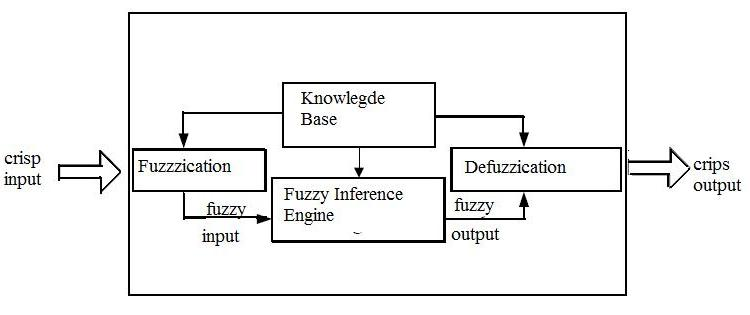
\includegraphics[width=0.90\textwidth]{"Part 2 - Search-Based Optimization/Particle Swarm Optimization/Images/Fig. 1.8.png"}
\caption{Fuzzy inference system}
\label{fig:FUZZY}
\end{figure}

\begin{itemize}
\item A \textit{knowledge base} containing a number of fuzzy if-then rules and the definitions of the memebership functions of the fuzzy sets used in the fuzzy rules.
\item A \textit{fuzzy inference engine} which performs the inference operations based on the fuzzy rules.
\item A \textit{fuzzification interface} that transforms the crisp inputs into degrees of match with linguistic values.
\item A defuzzification interface which transforms the fuzzy results of the inference into a crisp output.
\end{itemize}


The authors of the paper \cite{shi2001fuzzy} published in 2001 proposed to adapt $PSO$ by using a fuzzy system to adjust the inertia weight dynamically. 
%at four different levels: environment, population, individual, and component level. 
As mentioned previously, the inertia weight is an important parameter in PSO, since it affect the convergence and exploration-exploitation trade-off in PSO process. As the inertia weight is a global variable, it can be applied to the whole population. %A fuzzy system is basically an environment composed of if-then rules that determine the operation of the environment \cite{shi2001fuzzy}. 
The authors thus designed a fuzzy system to adapt the inertia weight dynamically as a global variable. 
The fuzzy system's input variables are the performance of the best candidate solution found so far by the PSO in normalised format and the current inertia weight, whereas the output variable is the change in inertia weight. %The current best performance evaluation named $CBPE$ indicates the best solution found by the $PSO$. Due to the wide variety of optimization problems, this term must be converted into a normalized format called $NCPBE$. Assume that we wish to solve a minimization problem and that the actual minimum is denoted $CBPE_{min}$ and the non-optimal $CBPE$ is denoted $CBPE_{max}$, which represents any suboptimal solution. % that is equal to or greater than $CBPE_{max}$. 
%The normalized $CBPE$ ($NCBPE$) can be computed as three fuzzy variables in order to 
All variables are associated to three fuzzy sets: low, medium, and high with associated membership functions as $left\_triangle$, $triangle$ and $right\_triangle$, respectively. The definitions of these three membership functions are: 

\begin{equation}
    f_{left\_triangle}=
    \begin{cases}
    1 & \text{if $x < x_1$}\\
    \frac{x_2 -x}{x_2 -x_1} & \text{if $x_1 \leq x \leq x_2$}\\
    0 & \text{if $x > x_2$}
    \end{cases}
\end{equation}

\begin{equation}
    f_{triangle}= \begin{cases}
    0 & \text{if $x<x_1$}\\
    2 \frac{x - x_1}{x_2 -x_1} & \text{if $x_1 \leq x \leq \frac{x_2 +x_1}{2}$}\\
    2 \frac{x_2 -x}{x_2 -x_1} & \text{if $\frac{x_2 +x_1}{2} < x \leq x_2$}\\
    0 & \text{if $x > x_2$}
    \end{cases}
\end{equation}

\begin{equation}
    f_{right\_triangle} = \begin{cases}
    0 & \text{if $x < x_1$}\\
    \frac{x -x_1}{x_2 -x_1} & \text{if $x_1 \leq x \leq x_2$}\\
    1 & \text{if $x > x_2$}
    \end{cases}
\end{equation}

\noindent where $x_1$ and $x_2$ are critical parameters that determine the shape and location of the functions. Other definitions of membership functions are possible, but the authors have found that the ones they proposed are useful for various problems and are easy to implement on microcontrollers and microprocessors.

\subsection{Major PSO variants for multi-objective optimization}
\label{sec:variants2}

PSO is a powerful tool for solving single-objective problems; for that reason, researchers expanded its capabilities to the multi-objective domain. The idea is to generate PSO-based approaches that can optimize more than one objective function. Assume a multi-objective optimization problem in the canonical form given in the introduction of Part II of this book:

\[
\begin{tabular}{ll}
minimize        & $f_k(\mathbf{x})$, \ \ \ \ \ \ \ \ \ \ \ $k=\{1,2,\cdots,p\}$ \\ 
subject to      & $g_i(\mathbf{x}) \leq 0$, \ \ \ \ \ $i=\{1,2,\cdots,m\}$ \\
                & $h_j(\mathbf{x}) = 0$, \ \ \ \ \ $j=\{1,2,\cdots,n\}$ ,\\
\end{tabular}
\]

\noindent where $\mathbf{x} \in \mathcal{X}$ is the design variable being optimised, $p$ is the number of objective functions to be optimised, $m$ is the number of constraints of the type $g_i$ and $n$ is the number of constraints of the type $h_j$. 
Multi-objective optimization (MO) aims to find a set of solutions called a Pareto set \cite{coello2007evolutionary}, where each solution is non-dominated by any other solution in the search space. A solution $\mathbf{x}^{(1)}$ is said to dominate another solution $\mathbf{x}^{(2)}$ if and only if:

\begin{equation}
\begin{tabular}{l}
$\forall i, f_i(\mathbf{x}^{(1)}) \leq f_i(\mathbf{x}^{(2)})$  and  \\
$\exists i, f_i(\mathbf{x}^{(1)}) < f_i(\mathbf{x}^{(2)})$ \label{eq:dominance}
\end{tabular}
\end{equation}

As such, the Pareto set can be seen as composed of solutions that represent different trade-offs among the objectives. This section briefly discusses the most relevant versions of the PSO for MO problems. These variants were selected based on their citations in scientific repositories.

\subsubsection{MOPSO} 

This algorithm proposed in 2002 introduces concepts of multiobjective optimization to modify the original PSO algorithm and implement it to solve multiobjective optimization problems. The authors named this approach MultiObjective Particle Swarm Optimization (MOPSO)~\cite{coello2002mopso} and validated it by comparing it with algorithms such as Pareto Archived Evolution Strategy (PAES)~\cite{knowles1999pareto} and the Non-dominated Sorting Genetic Algorithm II (NSGA II)~\cite{deb2000fast}.
%
%The analogy of the particle swarm with evolutionary algorithms made it evident that this algorithm could be designed for a multi-objective approach. Introducing concepts such as the Pareto front and using a memory known as a global repository in which each particle will deposit its flight experiences after each cycle to establish dominance degrees. Another adapted mechanism was that each particle could choose a different leader to perform the search and is based on the generation of hyper-cubes, which allows dividing the search space into already explored spaces; 
%
The general structure of the MOPSO algorithms is listed below:

\begin{enumerate}
    \item Initialize population with random position and velocity vectors.
    \item Evaluate the objective values of each particle. %, with their respective constraints and bounds $lb$ and $ub$ using the Eq.~\ref{eq:mo_criterion}.
    \item Archive=non-dominated solutions found so far.
    \item Determine the personal best of each particle.
    \item Apply Eqs.~\ref{eq:equation2} and~\ref{eq:equation3}.
    \item Repeat steps 2 to 6 until the stop criterion is reached.
\end{enumerate}

%\begin{equation}
%\begin{split}\label{eq:mo_criterion}
%    \text{Minimize/Maximize } f_n (x) &,\quad n=\{1,2,\cdots,O\}\\
%    \text{Subject to } g_j(x) \geq &, \quad j = \{1,2,\cdots,J\}\\
%    h_k(x)=0 &, \quad k=\{1,2,\cdots,K\}\\
%    x_i^{(lb)} \leq x_i \leq x_i^{(ub)} &, \quad i=\{1,2,\cdots,N\}
%\end{split}
%\end{equation} 


In MOPSO the velocity and position update equations remain similar to Eq.~\eqref{eq:equation2} and Eq.~\eqref{eq:equation3} of PSO, but the personal best and global best are computed differently. The personal best is determined based on the non-dominance concept. If the new position of a particle dominates the previous personal best of this particle, the new position replaces the previous personal best. If the previous personal best dominates the new position, then the previous personal best is kept. If the new position and the previous personal best are non-dominated by each other, one of them is chosen uniformly at random to become (or remain) the personal best of this particle. The global best is randomly selected among the non-dominated solutions from the archive by giving higher chance to select solutions located in less crowded regions of the search space, i.e., in regions where there are few archive solutions. 

This multi-objective algorithm has been widely used in the literature for applications in different fields; three of the most notable fields, according to the reports in~\cite{lalwani2013comprehensive} are Electrical Engineering, Industrial Engineering, Flow-shop, and Job-shop Scheduling.

\subsubsection{SMPSO}

In 2009, Nebro et al.~\cite{nebro2009smpso} studied six representative variants of MOPSO and found that they had problems solving multi-modal problems, i.e., problems with two or more optimal solutions. The problem was the ``swarm explosion"~\cite{clerc2002particle}: erratic movements toward the upper and lower boundaries of particle positions that occur when particles acquire very high velocity. Based on a MOPSO algorithm, they presented in~\cite{nebro2009smpso} a new multi-objective PSO algorithm using the velocity constraint strategy~\cite{clerc2002particle}. Their proposal could obtain proper particle positions when high velocity was present, avoiding the swarm explosion effect. The new algorithm, called Speed-constrained Multi-objective PSO (SMPSO), uses the following equations to adjust the velocity of the particles:

\begin{equation} \label{eq:con_coe}
\chi = \frac{2}{2 -\varphi - \sqrt{\varphi^2 -4\varphi}}
\end{equation}
\noindent where
\begin{equation}
\varphi = \left\{ \begin{matrix}
    c_1 + c_2 & \rm{if} \quad c_1 +c_2 > 4 \\ 
    1 & \rm{if} \quad c_1 +c_2 \leq 4
\end{matrix} \right.
\end{equation}
\noindent where $c_1$ and $c_2$ are the parameters to control the effect of the personal and global best particles.
Once the velocity of the particles is calculated in the original form ~\cite{nebro2009smpso}, it is multiplied by the constriction coefficient $\chi$, which helps to enable diverse solutions so that exploitation is not too much intensified. Then,
the velocity is constrained by Eq.~\ref{eq:vel_con}: 

\begin{equation} \label{eq:vel_con}
v_{i, j}^t = \left\{ \begin{matrix}
    \Delta b_j & {\rm if} \, v_{i,j}^t > \Delta b_j\\
    -\Delta b_j & {\rm if} \, v_{i,j}^t \leq -\Delta b_j\\
    v_{i,j}^t & {\rm otherwise}
\end{matrix} \right.
\end{equation}
\noindent where
\begin{equation}
    \Delta b_j = \frac{(ub_j -lb_j)}{2}
\end{equation}
\noindent where $ub$ and $lb$ are the upper and lower boundaries of search space defined by $\mathcal{X}$, and $\Delta b_j$ is the center point between them.
By implementing this strategy, SMPSO overcomes the swarm explosion effect of MOPSO algorithms. 
They reported that the approximations to the Pareto front found by their algorithm were better than the MOPSO algorithms. The SMPSO was the fastest algorithm converged to the Pareto front in their experiments.

\subsubsection{FC-MOPSO}

This algorithm presented in 2017~\cite{mokarram2018new} originally targeted at the problem of multi-objective design of engineering problems with few function evaluations.
%The main contributions are the following:
%\begin{itemize}
%    \item Effective leader selection process for each particle to guarantee diversity and fast convergence.
%    \item The FC-MOPSO is a modified algorithm for handling discrete optimization problems.
%    \item Use of constant value close to unity: $\alpha = 0.9.$.
%\end{itemize}
It generalizes the concept of personal best $\vec{lB}_i^t$ to the set $P_i$, which contains all non-dominated solutions found so far by the particle $i$. A particle called $\vec{psel}_i$ is selected from $P_i$ for the purpose updating the velocity (and position) of the particle $i$ in the algorithm. Similarly, the concept of local best $\vec{lB}_i$, which is used by some PSO variants to capture the best particle found in the neighbourhood of particle $i$ instead of in the population of particles as a whole, is also generalized to randomly select non-dominated solutions. 

The authors also suggest that FC-MOPSO starts with random velocities no greater than $v_{m} = 0.1(ub - lb)$, where $ub$ and $lb$ are the upper and the lower boundaries of the search space defined by $\mathcal{X}$, respectively. In other words, they prevent the method from starting with large velocities while starting with some speeds to start the search at a more advanced stage. 

%lgorithms should use the package algorithmic. An example is given below:


%%%%%%%%%%%%%%%%%%%%%%%% ALGORITHM
%\begin{algorithm}[ht!]
	%\renewcommand{\baselinestretch}{0.8}
%	\caption{Example algorithm}
    
 %   Parameters: enter parameters here
    
  %  Output: enter output here.
    
%	\begin{algorithmic}[1] 
%		\STATE{Do this.}
		
%        \REPEAT
		
%		\FOR{each model $m$}
		
%		\STATE Do that.
				
%		\ENDFOR
%		\UNTIL the maximum number of iterations is reached
		
%	\end{algorithmic}
	
%\end{algorithm}
%%%%%%%%%%%%%%%%%%%%%%%% ALGORITHM

\section{PSO Applications} \label{sec:apps}

The applications presented were chosen based on the relevance of current works consulted in the $Google Scholar$ repositories.\\
In recent years, robotics has undergone significant development. The specialization of many tasks requires the optimization of execution times and precision in the robot's movements.
In this sense, the modeling parameters of the robot were explored in~\cite{bingul2011dynamic}, where the researchers used a combination of the Least Square (LS) method and PSO to estimate a robotic arm's inertia parameters. The estimation performed by the algorithm matches closely with the manufacturer-provided values.
The trajectory planning for mobile
robots through PSO was implemented by Abdalla et al.~\cite{abdalla2017mobile}, Zeng et al.~\cite{zeng2016path}, and Wang et al.~\cite{wang2015trajectory}. Zeng et al. used a PSO based on a non-homogeneous Markov chain and Differential Evolution algorithm to generate a path into a space with obstacles for intelligent robots. Abdalla et al. proposed a combination of the artificial potential field (APF) with fuzzy logic, where PSO was used to optimize the membership functions of the fuzzy controller to acquire the mobiles robot trajectory, and Wang et al. combined the PSO algorithm with kinematics equations to trajectory planning in the free-floating space robot, simulating a couple of a spacecraft and a manipulator robot.

Electrical energy has been studied for centuries, and its use has been extended to all possible areas in recent decades. Now, with the renewable production of electrical energy, it is imperative to optimize its use and its distribution and production for maximum utilization.
Electricity sometimes came from a cascade system of hydroelectric generators. Evaporation, irrigation systems, and other factors affect the water level in the reservoirs. Mahor and Saroj~\cite{mahor2012short} used a PSO based algorithm to optimize the generation schedule of a real system of hydroelectric cascade system in India.
In \cite{bahrami2014short} Bahrami et al. use the PSO algorithm to determine the optimal parameter in a grey model. This model brings the opportunity to forecast the electric load in the short term, using minimal historical data. The method was used to forecast the load in Iran and New York electrical networks.
In 2016, Mesbahi et al. used a hybrid PSO-Nelder-Mead algorithm to identify and model electric vehicle batteries and then used this information to simulate vehicle energy demand, which allows maximum energy harvesting~\cite{mesbahi2016dynamical}. Finally, Mesbahi et al. compare their results against the power consumption of a physical urban electric vehicle, with a modeling error inferior to 0.5\%.
Mozafar et al. applied a multiobjective algorithm, using PSO combined with GA to optimize the location and capacity of renewable power sources and electric vehicle charging stations within the same distribution network.~\cite{mozafar2017simultaneous}.

\section{Conclusions}
\label{sec:conclusions}

The PSO is an interesting algorithm that has attracted the attention of researchers and practitioners from different areas over the years. The simplicity of the PSO makes it a popular mechanism for single-objective optimization. Their operators are easy to implement and permit finding solutions to complex problems. Since the PSO has been extensively used, it has also been modified to improve its performance.
Multi-objective problems require more sophisticated algorithms that permit handle with them.
In this sense, the PSO has been extended for multi-objective optimization. Regarding the importance of the PSO, it is possible to see how this method stills being a source of research from different repositories. The multiple modifications of the PSO algorithm are an excellent example of this. This chapter just considered the most relevant derivative work of PSO from 2010 to 2020. There exists more, but analyzing them is a complex and irrelevant task to the present work scopes. The quantity of derivative works is similar to the number of applications of the PSO; since its implementation is relatively easy and the code is entirely available, it is possible to find a significant number of articles that reports result from different fields of applications. It is possible to conclude that the PSO is one of the most important meta-heuristic algorithms, and the research related to it is still has lots to promise.

\subsection{Exercises}
\label{sec:exeercises}

\begin{enumerate}
    \item Program the Rosenbrock function defined as follows:
    
    \begin{equation} \label{eq:rosen}
    f(x_1 \cdots x_n) = \sum_{i=1}^{n-1} (100(x_i^2 - x_{i+1})^2 + (1-x_i)^2)
\end{equation}

\noindent where $-2.048 \leq x_i \leq 2.048$ and $\text{ the minimum at }f(1, 1, \cdots, 1) = 0$.  Once you have implemented the Rosenbrock function plot its surface in 2 dimensions.

    \item Considering the Rosenbrock function, initialize a random population of 50 particles and plot them in the the 2-dimensional surface of the function.
    
    \item Implement the standard version of the PSO explained in this chapter to minimize the Rosenbrock function. You need to obtain the curve of convergence of the best solution at each iteration and plot it.
    
    \item Implement a code of the Fully Informed PSO that was explained in this chapter. The Fully Informed PSO should be able to minimize the Rosenbrock function. Obtain the convergence curve and compare it with the one obtained by the standard PSO. 
    
\end{enumerate}

\subsection{Answers to the exercises}
\label{sec:answers}

\begin{enumerate}
    \item Rosenbrock function top view
    \begin{figure} [H]
    \centering
        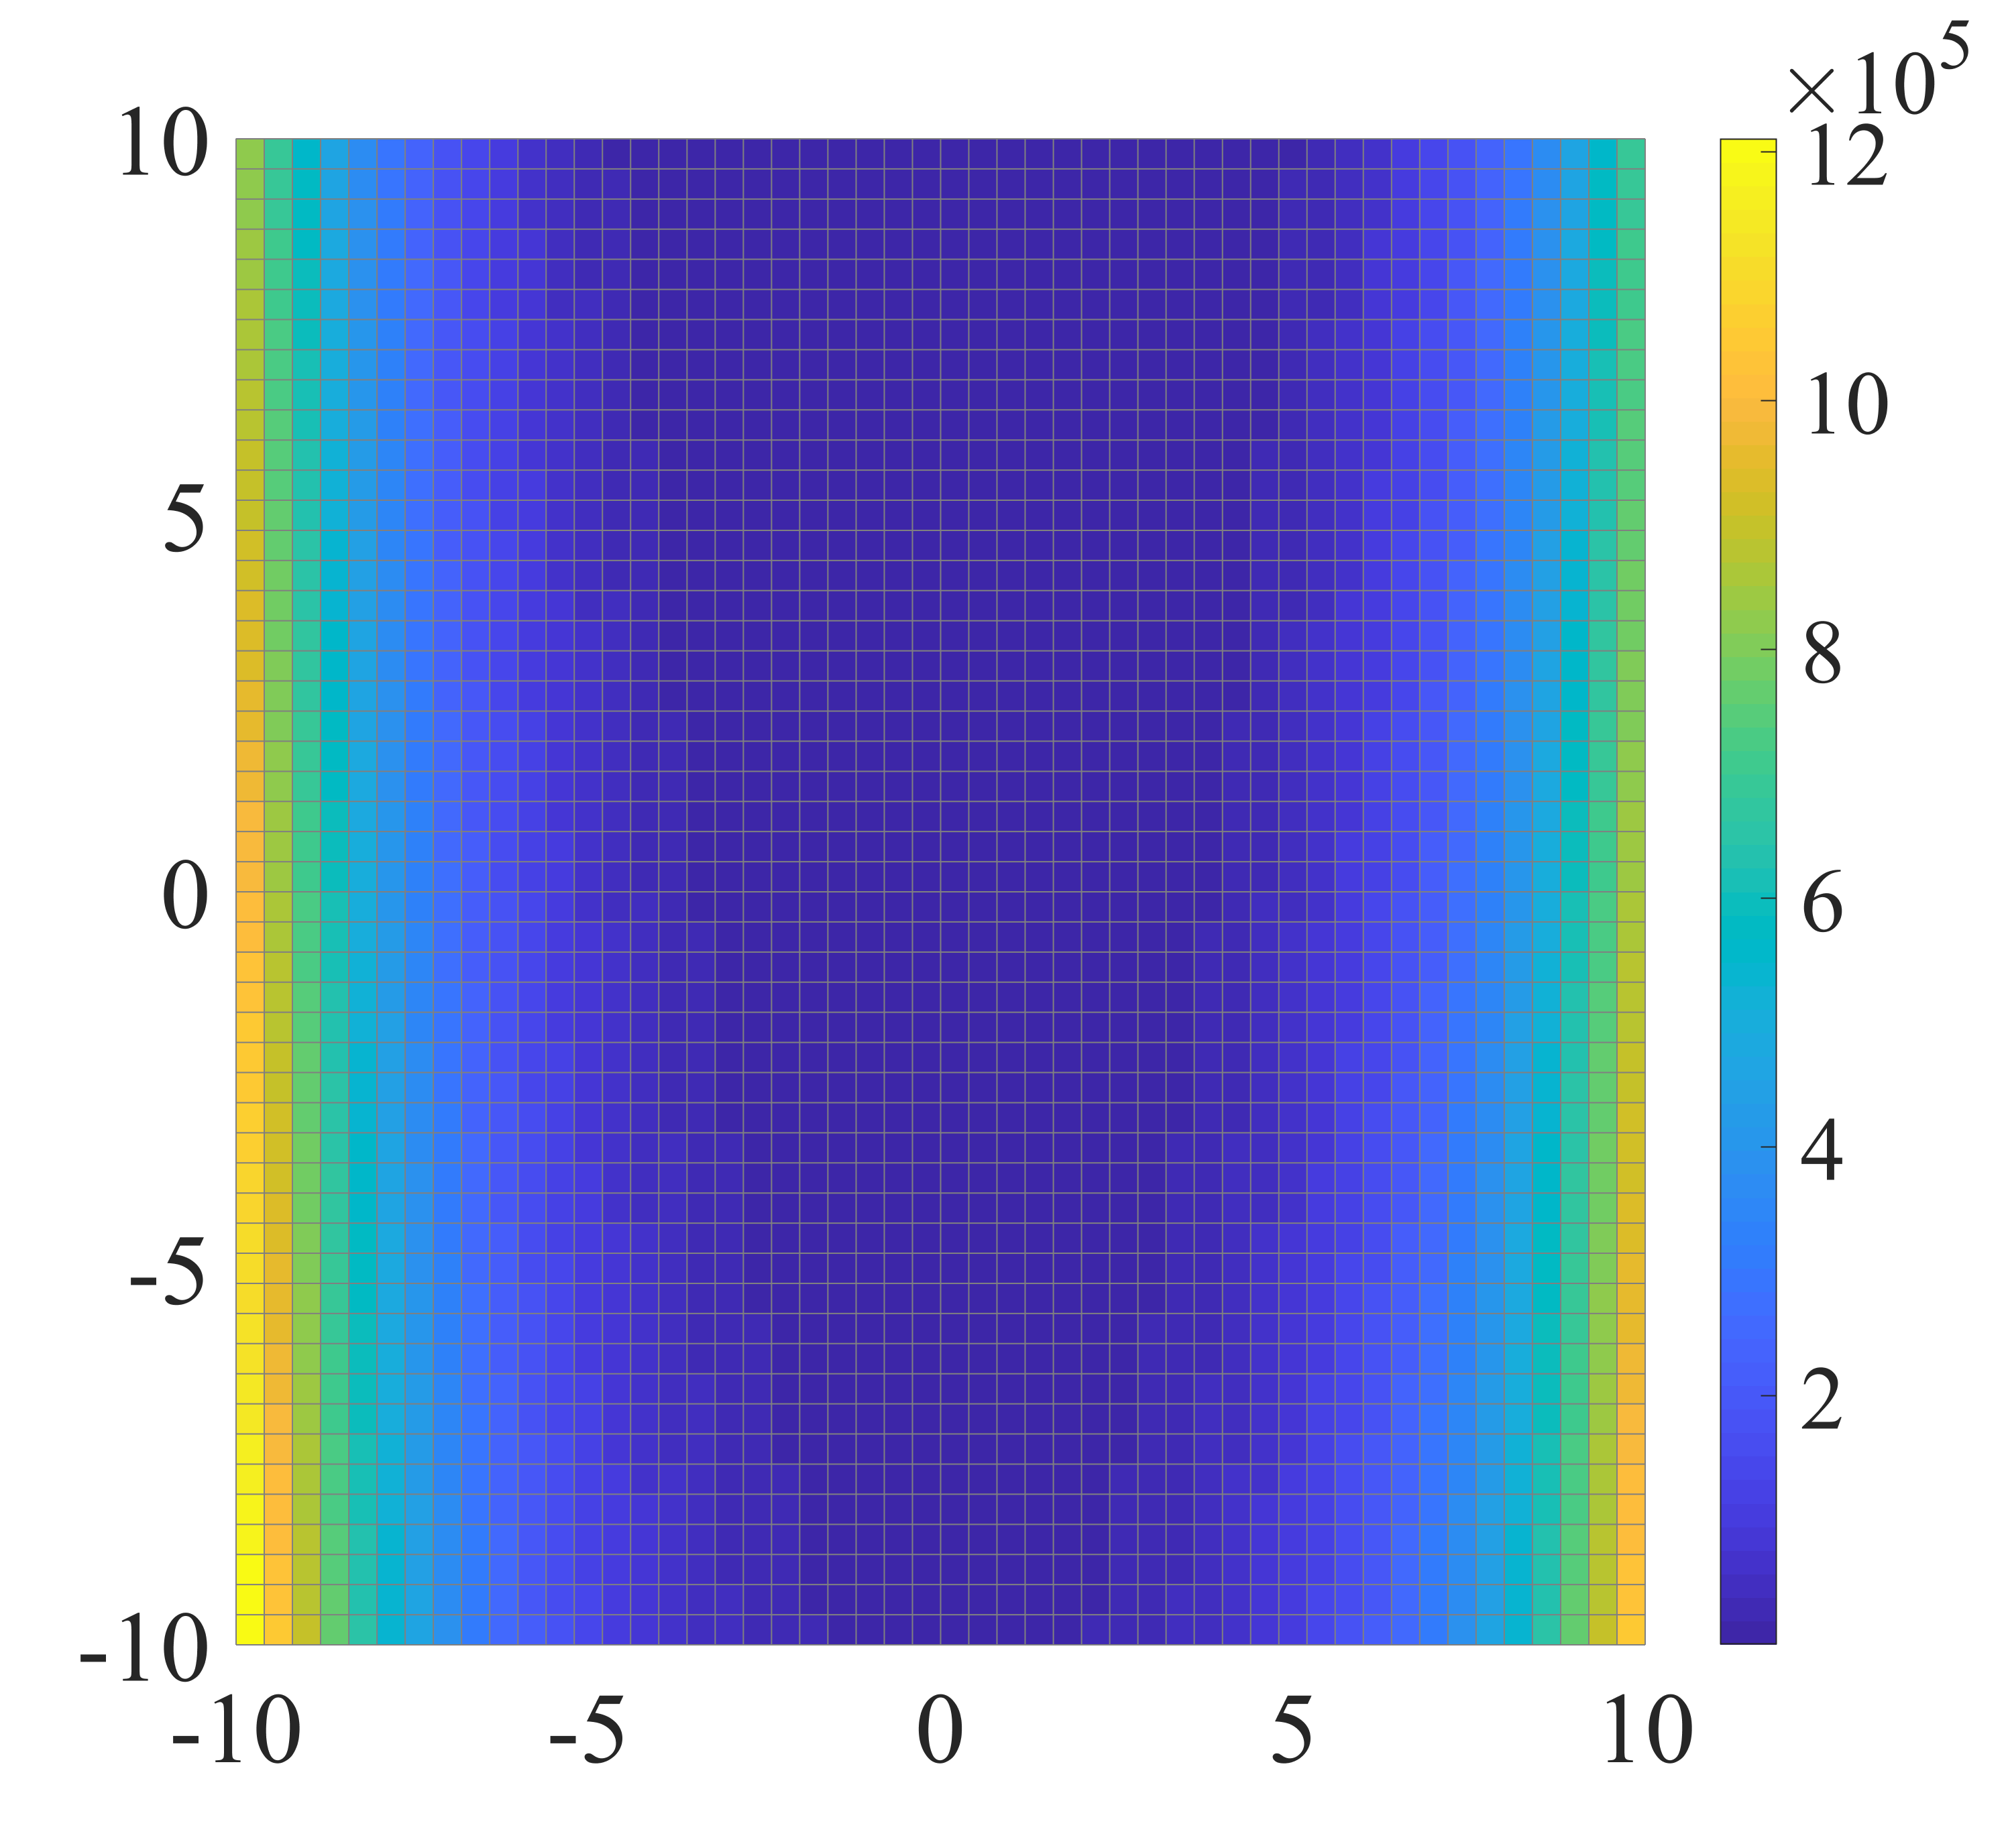
\includegraphics[width=0.60\textwidth]{"Part 2 - Search-Based Optimization/Particle Swarm Optimization/Images/rosenbrock.PNG"}
        \caption{Rosenbrock function}
        \label{fig:rosenbrock_function}
    \end{figure}
    
    \item initialization of a random population of 50 particles on the 2-dimensional surface of the Rosenbrock function.
    \begin{figure} [H]
    \centering
        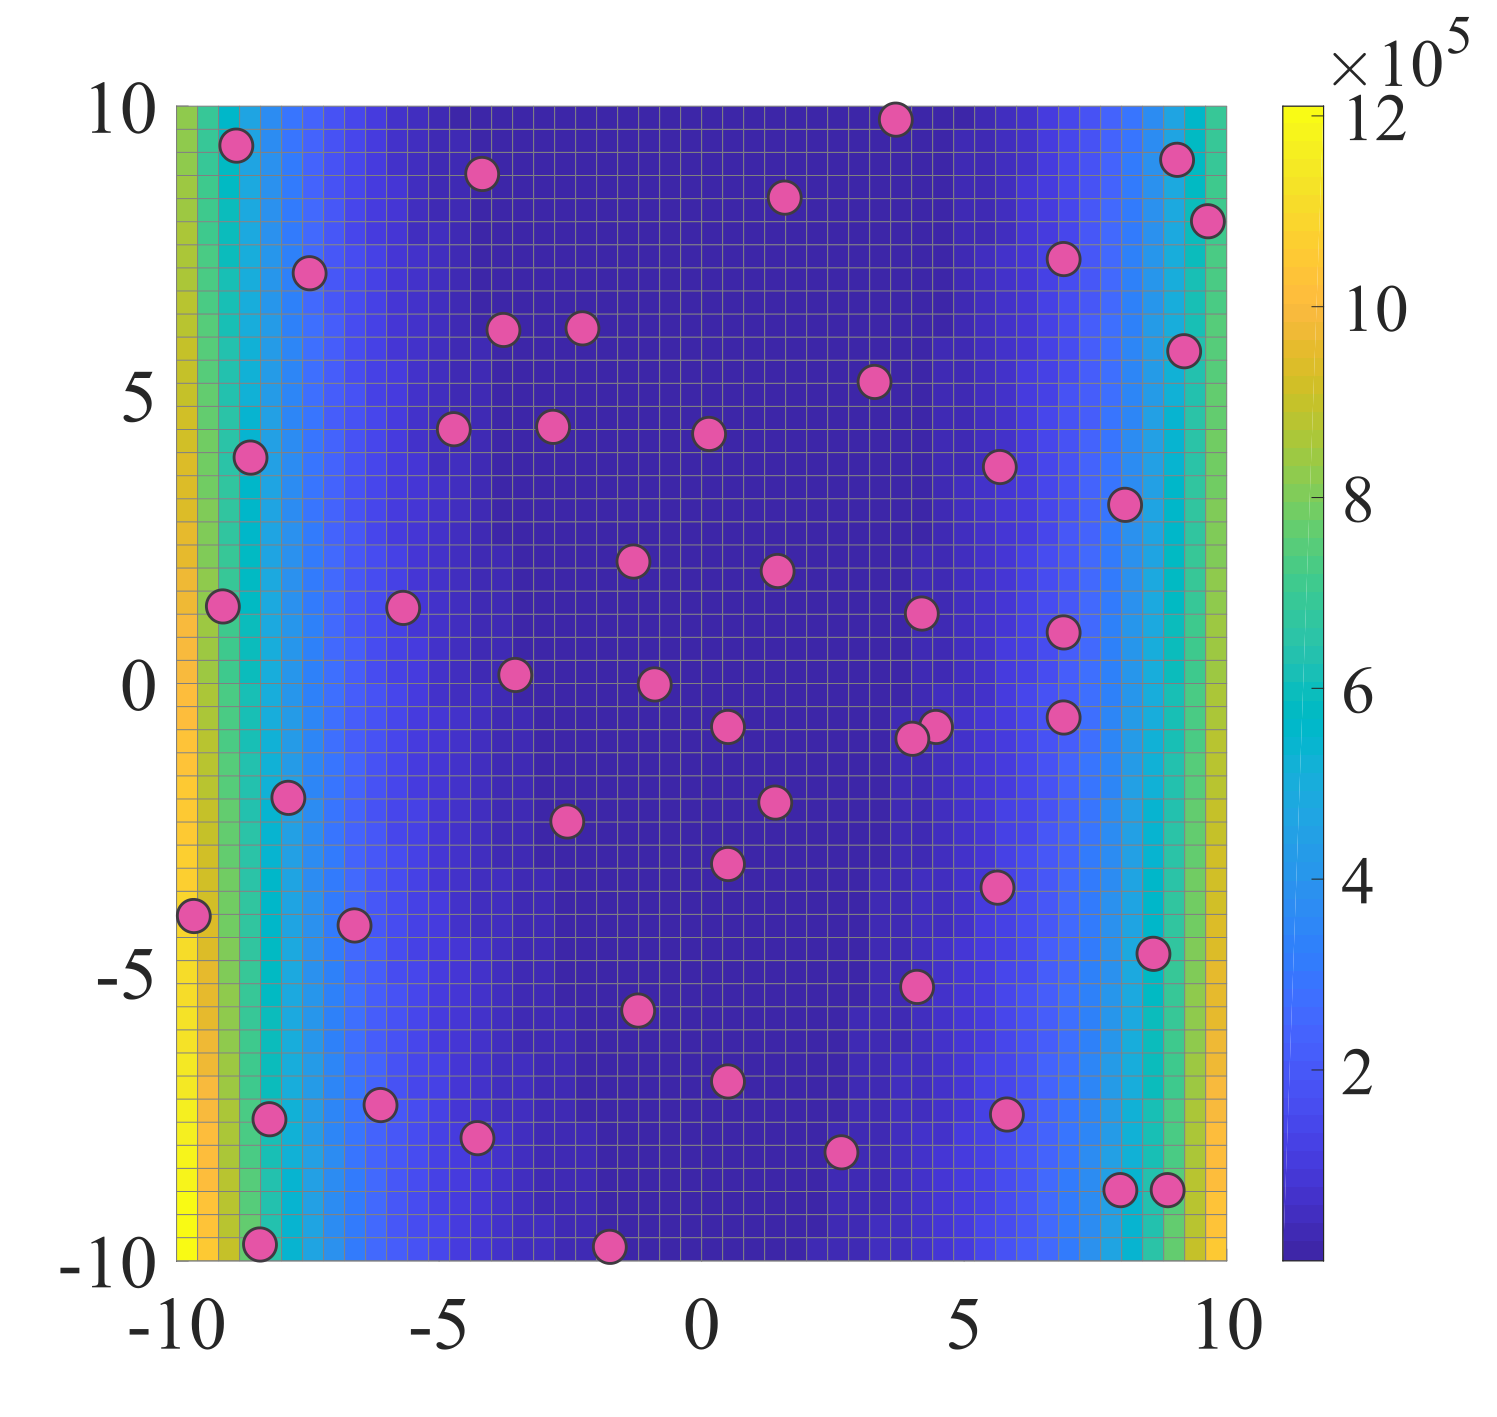
\includegraphics[width=0.60\textwidth]{"Part 2 - Search-Based Optimization/Particle Swarm Optimization/Images/rosenbrock_plot_particles.PNG"}
        \caption{Initialization of 50 particles on the Rosenbrock function}
        \label{fig:rosenbrock_function_inicializarion_particles}
    \end{figure}

    \item Convergence plot of standard particle swarm optimization version 
    
        \begin{figure} [H]
    \centering
        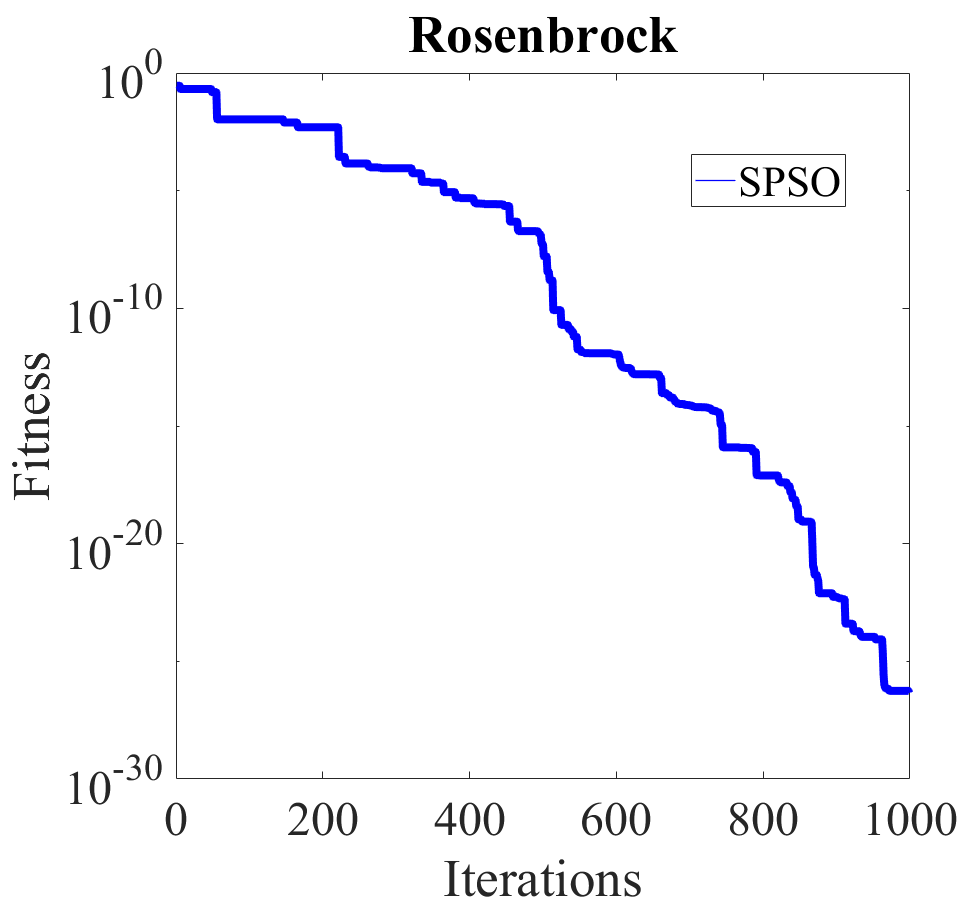
\includegraphics[width=0.60\textwidth]{"Part 2 - Search-Based Optimization/Particle Swarm Optimization/Images/SPSO.png"}
        \caption{SPSO convergence graph}
        \label{fig:SPSO_convergence_graph}
    \end{figure}
    
    \item Comparison of convergence plots between standard particle swarm optimization~(SPSO) and Fully informed Particle Swarm~(FIPS).
    
     \begin{figure} [H]
    \centering
        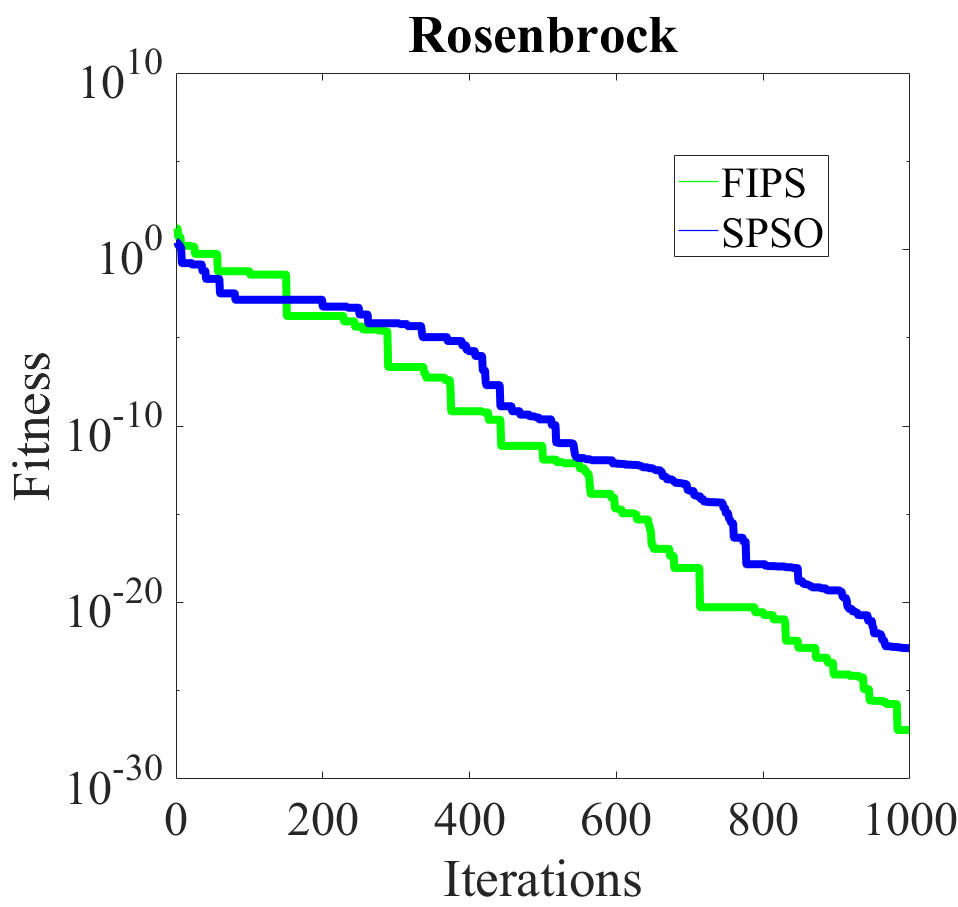
\includegraphics[width=0.60\textwidth]{"Part 2 - Search-Based Optimization/Particle Swarm Optimization/Images/VersusPS.png"}
        \caption{SPSO vs. FIPS convergence plots}
        \label{fig:SPSOvs.FIPS_convergence_plots}
    \end{figure}
    
\end{enumerate}



\bibliographystyle{unsrt}
\bibliography{bibliography}

\chapter{Other Search-Based Optimization Approaches}
\label{chp:other-search-based-optimization-approaches}


\title{Local Search}
\label{chp:local-search}
\author{Sara Ceschia, Luca Di Gaspero, Andrea Schaerf}
\institute{DPIA, University of Udine\\ 
\texttt{\{sara.ceschia,luca.digaspero,andrea.schaerf\}@uniud.it}}
\maketitle


\emph{Local Search} is an algorithmic paradigm for combinatorial
search and optimization, which has been shown to be very effective for many
problems in the scientific literature. A large number
of techniques based on local search have been proposed to successfully
address a variety of practical problems.


Local search techniques belong to the larger class of the so-called
\emph{selective} methods that are based on the exploration of the
search space composed by complete solutions. This is opposed to
\emph{constructive} methods that build the solution in a step-by-step
manner by iteratively adding a new piece to the partial solution constructed
that far.  

In addition, local search techniques are non-exact, as they
do not guarantee to find the optimal solution. In the cases in which
the optimal solution is found, there is no way to prove that it is
indeed optimal, unless it has been established
with exact techniques that it is not possible to reach a value lower than that (i.e., it is a proven \emph{lower bound}).

Local search is based on the simple idea of \emph{navigating} the
search space by iteratively stepping from one state to one of its
\emph{neighbors}. The neighborhood of a state is the set of states
that can be obtained by applying a ``local change'' to it. The
definition of the neighborhood relation is dependent on the specific
problem under consideration, although there are some common
patterns that can be applied to search spaces with
similar structure.  The mechanism upon which the neighbor is selected
at each step is one of the main design choices that varies
among different local search techniques. In any case, this selection
mechanism relies upon the definition of the \emph{cost function} $F$,
which assesses the quality of each neighbor state, and it is also
problem dependent.

% NEW PARAGRAPH
Even though it is difficult to assess precisely when local search should be 
used instead of other optimization methods, a general observation is that 
its behavior depends on the landscape of the cost function. More precisely, if the 
landscape is relatively \emph{smooth} with respect to local 
changes, it is more likely that local search techniques will be successful.


In this chapter, we discuss the key elements of the local
search paradigm, which are independent of both the specific problem 
and the specific local search technique chosen to solve it.

We also introduce the basic local search techniques and discuss some
improvements and variations of such basic methods. We refer to
the following chapters %Chapter~\ref{cap:simulated-annealing} 
and the book by Hoos and St\"utzle \cite{HoSt05} for more complex local search
techniques. % others?



\section{Local Search Elements}

We first introduce one by one the key elements of local search.  In
detail, we will introduce the notions of \emph{search space},
\emph{neighborhood relation}, \emph{cost function}, \emph{initial
  solution selection}, \emph{move selection and acceptance criterion},
and \emph{stop criterion}.

\subsection{Search Space}

Given a search or optimization problem $P$ and an instance $I$ of $P$, we
associate to it a search space $S$, with the following properties:

\begin{itemize}
\item each element $s\in S$ represents a solution of $I$, not
  necessarily feasible (i.e., it might violate some constraint of the problem);
\item for search problems, at least one feasible solution of $I$ is
  represented in $S$;
\item for optimization problems, at least one optimal solution of $I$
  is represented in $S$.
\end{itemize}

If the previous requirements are met, we have a \emph{valid
  representation} of the problem. We refer to an element $s\in S$ as a
\emph{state}.

% Q: is n-queens already defined?
Consider for example the classical $n$-queens problem, which consists
in placing $n$ queens in an $n\times n$ chessboard so that they do not
attack each other neither vertically, nor horizontally, nor diagonally.

The direct representation of the problem would be with an $n\times n$
matrix of boolean-values, each representing the presence/absence of a
queen in the corresponding square. However, the intuitive search
spaces for local search already partition the chessboard in columns,
making use of $n$ integer-valued variables $\mathbf{x} = [x_1, x_2,
\dots, x_n]$ such that the assignment $x_i = j$ corresponds to place a
queen in position $(j,i)$ in the chessboard. Since this representation
places only one queen in each column, it implicitly provides against
vertical attacks.

There are two typical options for the definition of the
search space for the $n$-queens problem:

\begin{itemize}
\item \textbf{Assignment}: any variable $x_1,\dots, x_n$ can assume
  any value in the domain $\chi = \{1,\dots,n\}$. 
\item \textbf{Permutation}: variables can assume only distinct values in the domain $\chi = \{1,\dots,n\}$, resulting in a permutation of the numbers $1,\dots,n$. 
\end{itemize}

For example, $\mathbf{s_1} = [4,6,1,6,8,4,2,1]$ is a state for the instance with
$n = 8$ for \textbf{Assignment}, and $\mathbf{s_2} = [4,1,7,6,8,3,2,5]$ is a
state for both search spaces. These states are depicted in Figures~\ref{fig:nqueens-assignment} and \ref{fig:nqueens-permutation}.
% replace il the figure X with s_1 and s_2 (LUCA)

\begin{figure}
  \subfigures 
  \begin{minipage}{\textwidth}
    \leftfigure[t]{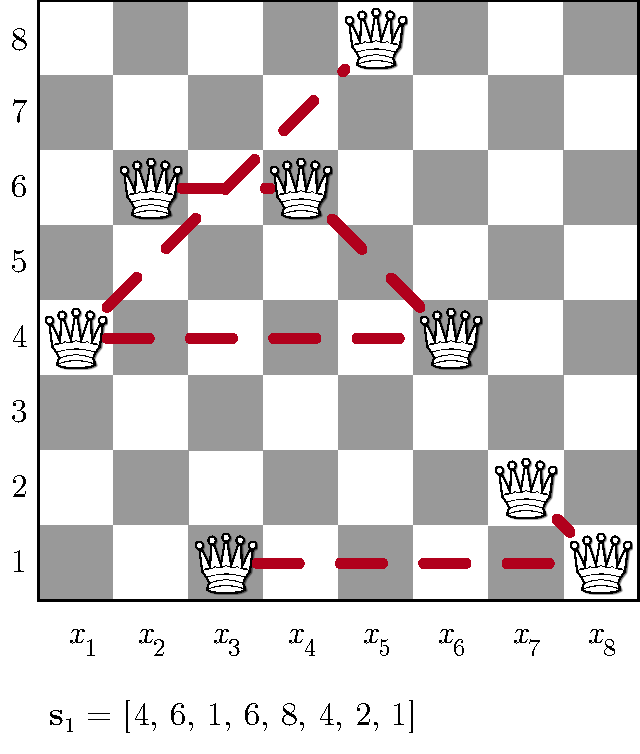
\includegraphics[width=0.4\textwidth]{"Part 2 - Search-Based Optimization/Local Search/n-queens/assignment.pdf"}}
    \hspace{\fill}
    \rightfigure[t]{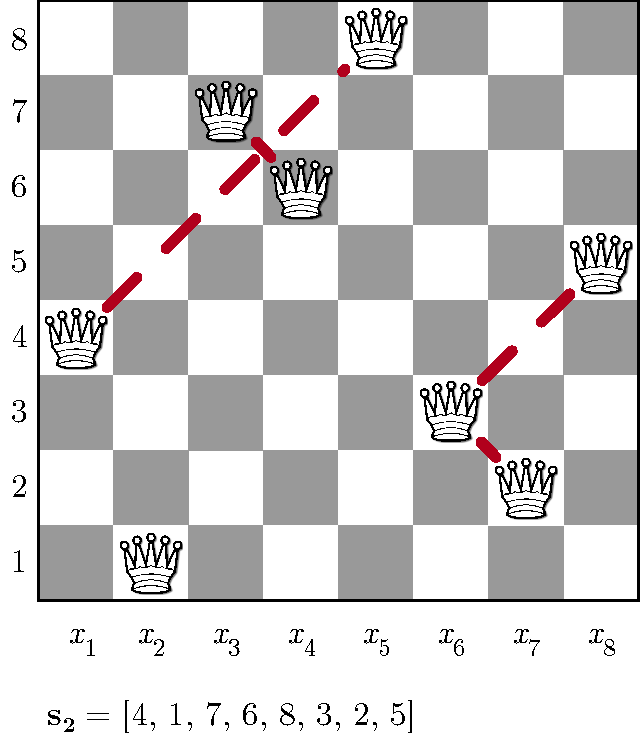
\includegraphics[width=0.4\textwidth]{"Part 2 - Search-Based Optimization/Local Search/n-queens/permutation.pdf"}}
  \end{minipage}
  \leftcaption{A state for the $n$-queens problem in the \textbf{Assignment} search space. \label{fig:nqueens-assignment}}
  \rightcaption{A state for the $n$-queens problem in the \textbf{Permutation} search space (and also in the \textbf{Assignment} one). \label{fig:nqueens-permutation}}
\end{figure}

In the \textbf{Assignment} space, horizontal and diagonal attacks have
to be taken care by the cost function $F$. In the \textbf{Permutation}
space, instead, since the search space is restricted so that two variables
cannot have the same value, also horizontal attacks are prevented by construction. In
this case, the only possible constraint violations come from the
diagonal attacks. It is easy to see that both choices are valid representations in the
sense defined above.

\subsection{Neighborhood Relation}

Given a problem $P$, an instance $I$ and a search space $S$ for it, we
assign to each element $s\in S$ a set $\mathcal{N}(s) \subseteq S$ of
neighboring states of $s$. The set $\mathcal{N}(s)$ is called the
\emph{neighborhood} of $s$ and each member $s'\in \mathcal{N}(s)$ is
called a \emph{neighbor} of $s$.

The set $\mathcal{N}(s)$ does not need to be listed explicitly, but usually
it is implicitly defined by referring to a set of possible
\emph{moves}, which define transitions between states. A move $m$
is defined by a small set of attributes that describe local
modifications of some parts of $s$. We call $s \oplus m$ the state
obtained by the application of move $m$ to state $s$. The ``locality''
of moves is the key ingredient of local search, and it has
also given the name of the whole search paradigm. Nevertheless, from
the definition above there is no implication that there is
``closeness'' in some sense among neighbors, and in fact complex
neighborhood definitions can be used as well.

The only condition that needs to be imposed on the neighborhood relation
$\mathcal{N}$ is that the search space $\mathcal{S}$ is connected
under $\mathcal{N}$. That is, every state $s$ of $\mathcal{S}$ can be
reached from any other state $s'$ by a finite-length sequence of moves
coming from $\mathcal{N}$.

Following the $n$-queens example, we consider two possible
neighborhood relations:

\begin{itemize}\itemsep 2mm
\item \textsf{Change} (\textsf{C}), for \textbf{Assignment} search space:\\
  The move \textsf{C}$\langle q,v\rangle$ assigns value $v$ to variable $x_q$.\\
  \underline{Precondition:} $x_q \neq v$.\\
%  \underline{Example:}   $[3,4,1,7,8,\textbf{4},2,1] \oplus \textsf{C} \langle 6, 1\rangle ~\rightarrow~[3,4,1,7,8,\textbf{1},2,1]$ \\
  
\item \textsf{Swap} (\textsf{S}), for \textbf{Permutation} search space:\\
The move \textsf{S}$\langle q_1,q_2\rangle$ swaps the  values assigned to variables $x_{q_1}$ and $x_{q_2}$.\\
\underline{Precondition:} $q_1\neq q_2$.\\
%\underline{Example:} $[4,\textbf{3},6,5,2,\textbf{1},8,7] \oplus \textsf{S}\langle2, 6\rangle~\rightarrow~[4,\textbf{1},6,5,2,\textbf{3},8,7]$ \\
\end{itemize}

See Figures~\ref{fig:nqueens-change} and~\ref{fig:nqueens-swap} for an example of each move, where the black arrows represent the transitions.

\begin{figure}
  \subfigures 
  \begin{minipage}{\textwidth}
    \leftfigure[t]{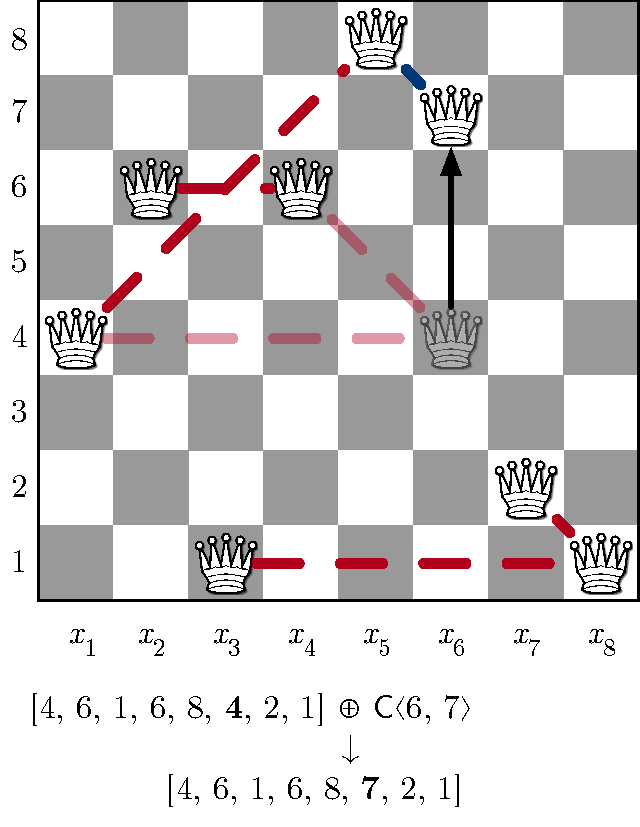
\includegraphics[width=0.4\textwidth]{"Part 2 - Search-Based Optimization/Local Search/n-queens/assignment_change.pdf"}}
    \hspace{\fill}
    \rightfigure[t]{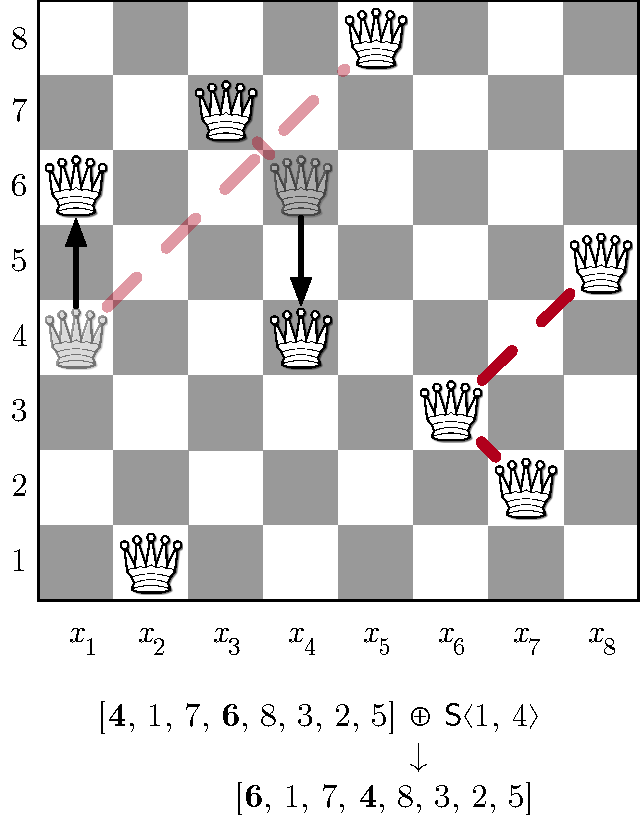
\includegraphics[width=0.4\textwidth]{"Part 2 - Search-Based Optimization/Local Search/n-queens/permutation_swap.pdf"}}
  \end{minipage}
  \leftcaption{An example of \textsf{Change} move. \label{fig:nqueens-change}}
  \rightcaption{An example of \textsf{Swap} move. \label{fig:nqueens-swap}}
\end{figure}


Notice that the \textsf{Change} neighborhood could not be applied to
the \textbf{Permutation} search space, as the moves would lead outside
the search space by duplicating some values. The \textsf{Swap}
neighborhood, instead, can also be applied to the \textbf{Assignment}
search space, but the space would not be connected under this
neighborhood, as the number of repetitions of each value does not
change upon the application of \textsf{Swap} moves, so that certain
states (with different number of repetitions) are never reached.

Nowadays there is a large body of scientific literature that shows the
effectiveness of different neighborhoods on the various problem
domains (e.g., routing and scheduling \cite{IIKM05}).
Nonetheless, the definition of a suitable neighborhood for the
specific novel problem remains a creative activity that the designers
have to undertake using their own intuition and experience. The proof
that the search space is connected under a specific neighborhood is
also a designer's task, which however is relatively easy to do for
most problems. For example, for the $n$-queens problem, for the two
proposed combinations of search space and neighborhood, it is rather
trivial to show that the search space is connected.

One of the key features of the design of the neighborhood relation is
the possibility to compute efficiently the so-called \emph{delta}
function, which is the cost difference between two neighbor states.
For example, for a \textsf{Change} move for the $n$-queens problem,
only the attacks created (resp.\ removed) by the presence in the new
(resp.\ old) position of the specific queen involved in the move needs
to be evaluated. This is easily done in linear time (with respect to
$n$). On the contrary, the full evaluation of the new state obtained
by applying the move would have a quadratic computational cost.

\subsection{Cost Function}

The selection of the move to be performed at each step is based on the
\emph{cost function} $F$ that associates to each element $s\in S$ a
value $F(s)$ that assesses the quality of the solution. For the sake
of simplicity, we assume that the value of $F$ is integer-valued and
non-negative, or in other words, that the co-domain of $F$ is the set
of natural numbers $\mathbb{N}$.

When applied to search problems, the function $F$ normally counts the
number of constraint violations, which is also known as 
\emph{distance to feasibility}. For example, in the $n$-queens
problem, the customary cost function counts the number of attacking
pairs of queens. For the state $s_1 = [4,6,1,6,8,4,2,1]$ 
represented in Figure~\ref{fig:nqueens-assignment},
we have $F(s_1) = 6$, as there are 6 pairs of queens attacking each
other $\{(x_1,x_5), (x_1,x_6), (x_2,x_4), (x_3,x_8),  (x_4,x_6),  (x_7,x_8)\}$ 
connected in the figures with red dotted lines.\footnote{Note that we count also the so-called \emph{X-ray} attacks, i.e. the ones between non consecutive queens in a row (or diagonal) of more than two of them, which by the chess rules would not attack each other.}

In the case of an optimization problem (which, without loss of
generality, is assumed to be a minimization one), $F$ typically merges
together the distance to feasibility and the objective function $f$ of
the problem.  Therefore, the cost function is typically defined as a
weighted sum, with the highest weight assigned to the distance to
feasibility, so as to give preference to feasibility over
optimality. % It seems that optimality is neglected, I would try to rephrase
%
An alternative option is to do not assign weights, but rather consider
the cost function as a pair, and perform the comparison of values in a
hierarchical way, with priority assigned to feasibility.

For some optimization problems the search space can be defined in such
a way that it represents only feasible solutions, and in those cases the cost
function normally coincides with the objective function of the problem.

In some cases, the objective function is complemented by some
auxiliary components which account for ``invisible improvements'' that
incorporate some problem knowledge that is not explicitly considered
in the objective function.  These auxiliary components might be useful
to guide the search toward promising regions of the search space.
As an example of this concept, consider the bin-packing problem for
which the objective is to minimize the number of bins and the selected
neighborhood just moves one object from one bin to another. In this
case, it could be useful to include in the cost function an auxiliary
component that favors states in which bins are filled in an unbalanced
way, rather then a situation in which objects are equally distributed
in the bids. Indeed, such an auxiliary component could create a search
trajectory composed of improving moves leading towards the removal of
one bin. % citation? Sara's phd thesis? Sect 6.3.4

Finally, it is also possible that the cost function is a surrogate of
the real objective function in the case that the latter one is
computationally expensive~\cite{KoCL11}.

\subsection{Initial Solution Selection}

An essential component of any local search procedure is the selection of
the initial solution. Typical choices are a random
generation or the use of a greedy constructive heuristic. It is also possible to use any
other search method to obtain the initial solution.

For example, for the \textbf{Permutation} space for the $n$-queens, the
random state can be obtained by creating the identity permutation
$[1,2,\dots,n]$ and then shuffling it by using the Fischer
and Yates algorithm \cite{FiYa38}.


In order to decide whether to use just a random initial state or spend
some effort to search for a greedy one, we should take into account
different aspects. In fact, on the one hand, a better initial state
would in general require less local search iterations in order to reach
high quality solutions. This saves computational time, which could be used
to perform more steps or more independent runs. On the other hand,
though, it is also possible that the greedy heuristics biases the
search toward some specific regions of the search space, so that it
might become difficult to move away toward different areas.

In some cases, the greedy procedure might be necessary in order to
obtain an initial feasible solution that a random procedure would not
reach. This behavior would allows us to avoid to be forced to include
the distance to feasibility in the cost function by finding a feasible
initial solution, thus simplifying the cost function of the local
search procedure.

% in other cases (eg bin packing) a greedy heuristic finds an initial feasible solution that represents an upper bound, which is then improved by the iterative applying the local search procedure

%For some local search techniques the construction of the initial
%solution is part of the algorithm specification, and thus it is
%required to be done in a certain way.


\subsection{Move Selection and Acceptable Criterion}

At each search step, a single move is selected. The way this selection is
performed characterizes the specific local search strategy, and we
will discuss the different options in the following sections.

However, the selection of a specific move does not inevitably imply that
the move is \emph{accepted} and performed, so that the current state is changed. On
the contrary, the move is normally subject to an acceptance condition,
which is also dependent on the specific technique under consideration.

As a general rule, moves that improve (i.e., decrease) the cost function are
accepted, but also worsening moves (i.e., increasing ones) could be accepted in specific
situations, so as to let the search move away from a \emph{local minimum}.
A local minimum is a state $s$ such that $F(s) \leq F(s')$ for all $s'
\in \mathcal{N}(s)$. When this condition holds also with a strict inequality $<$, 
we call the state a \emph{strict} local minimum. Escaping from local minima is the key issue of all local search techniques.

\subsection{Stop Criterion}\label{sec:stop-criteria}

To end the presentation of the common key elements of local search
we discuss the stop criterion, which determines when the search
is over and the best solution found that far is returned.

Many criteria have been proposed in the literature, starting from the
basic ones, typically based on the expiration of a given amount of time, 
to more complex strategies (see for example \cite[Sect.~3.2]{FrSt19}).
The basic time-expiration strategies can either refer to the wall-clock time or to more
abstract temporal measures, such as the number of iterations. The latter one has the 
advantage of not being machine dependent.

Other options might regard specific qualities of the solution reached
or the so-called \emph{stagnation} detection. That is, when no
improvement is obtained for a given number of iterations, the search is
stopped.  This way, search trials that are exploring promising paths
are let run longer than those that are stuck in regions without good
solutions or where the search is trapped.  It is also possible to
combine different criteria, by stopping the search when the first of a
set of conditions is met.  Similarly to the initial solution
selection, the stop criterion can be part of the specific technique,
therefore we will further discuss it in the following sections.
\vspace{\parskip}

Combining all the key elements presented so far, the pseudocode of a generic local search procedure is shown in
Algorithm~\ref{alg:local-search-pseudocode}.

\begin{algorithm}[ht!]
    %\renewcommand{\baselinestretch}{0.8}
    \caption{LocalSearch} \label{alg:local-search-pseudocode}   
    Parameters: SearchSpace $\mathcal{S}$, Neighborhood $\mathcal{N}$, CostFunction $F$\\   
    Output: $s_{best}$
    \begin{algorithmic}[1]
            \STATE $s \gets InitialState(\mathcal{S})$
            \STATE $s_{best} \gets s$
            \WHILE{\NOT{$StopCriterion$}}
                \STATE $m \gets SelectMove(s,\mathcal{N})$
                \STATE $\Delta F \gets F(s \oplus m) - F(s)$
                \IF{$AcceptMove(m,\Delta F)$}
                    \STATE $s \gets s \oplus m$
            \IF{$F(s) < F(s_{best})$}
                \STATE  $s_{best} \gets s$ \\
            \ENDIF
                \ENDIF
            \ENDWHILE
    \RETURN $s_{best}$
    \end{algorithmic}
\end{algorithm}

The specific definitions of the subprocedures $InitialState$, $StopCriterion$, $SelectMove$, and $AcceptMove$ characterize the specific local search technique.

%%%%%%%%%%%%%%%%%%%%%%%%%%%%%%%%%%%%%%%%%%%%%%%%%%%%%%%%%%%%%%%%%
\section{Basic Local Search Techniques}\label{sec:basics}
%%%%%%%%%%%%%%%%%%%%%%%%%%%%%%%%%%%%%%%%%%%%%%%%%%%%%%%%%%%%%%%%%

The simplest local search techniques are based on some
form of the so-called \emph{Iterative Descent} (also known as
\emph{Iterative Improvement} or \emph{Hill Climbing}).  The idea behind these 
techniques is to select at each step a move that improves the value of the objective
function or reduces the distance to feasibility, never
performing worsening moves.


\subsection{Steepest Descent}

The most well-known form of Iterative Descent is the so-called
\emph{Steepest Descent} (SD) technique. At each iteration, SD selects,
from the whole neighborhood $\mathcal{N}(s)$ of the current state
$s$, the element $s' = s \oplus m$ which has the best value of the
cost function $F$.  The SD procedure accepts the move $m$ only if it
an improving move, i.e., it decreases the value of the cost function. 
Consequently, it naturally stops as soon as it reaches a
local minimum. Therefore, assuming (as customary for combinatorial optimization) that the search space is finite and thus at least one local minimum exists, we don't need to define any other specific stop criterion.

The exhaustive exploration of the neighborhood is obtained by
enumerating the moves in a fixed order.  For example, the
\textsf{Swap} neighborhood for the $5$-queens problem, can be
enumerated in the following lexicographic order: $\{\langle 1,2\rangle, \langle
1,3\rangle, \langle 1,4\rangle, \langle 1,5\rangle, \langle
2,3\rangle, \langle 2,4\rangle, \langle 2,5\rangle, \langle
3,4\rangle, \langle 3,5\rangle, \langle 4,5\rangle\}$.

Notice that if there are two moves that lead to the same state, such as $\langle i,j\rangle$ and $\langle j,i\rangle$ in this case, only one of them should be included in order to prevent wasting time by visiting the same neighbor twice.

The enumeration of the neighborhood raises the issue of tie-breaking
in case of multiple solutions whose value of the cost function is equally good. 
The typical strategy is
to break ties in a uniform random way. That is, if there are $k$
neighbors with the same minimal cost, then each of them might be selected with
probability $1/k$.

\subsection{First-Improving Descent}


The exhaustive neighborhood exploration prescribed by the SD technique might be
rather expensive from the computational point of view. To overcome
this problem, the \emph{First-Improving Descent} (FID) technique accepts a move and moves
to a new neighbor as soon as an improving move is found. FID also
stops when there are no improving moves so that a local minimum is
detected.

In order to avoid the bias toward some specific attributes (e.g., the variables
with low indexes in the above example), the exploration of the
neighborhood should not proceed always in the same fixed order. The
simplest way to avoid such a bias is to start from a random move and
proceed onward in a circular way, by going from the last move to the first one. The procedure stops when the initial
random one is encountered again. For example, the exploration could proceed in the
following order $\{\langle 2,4\rangle,
\langle 2,5\rangle, \langle 3,4\rangle, \langle 3,5\rangle, \langle
4,5\rangle, \langle 1,2\rangle, \langle 1,3\rangle, \langle
1,4\rangle, \langle 1,5\rangle, \langle 2,3\rangle\}$ and stop as soon as an improving move has been found.

\subsection{Random Descent}

Another option to mitigate the computation burden of exhaustive neighborhood exploration 
consists in sampling the neighborhood by drawing random moves. This leads to
the \emph{Random Descent} (RD) technique that draws a (uniform) random move
at each iteration and performs it only if it is improving. 

Care should be taken to ensure that the draw is uniform. Drawing the attributes one at 
the time selecting among available values might bias the search toward moves 
that have a smaller number of possible values for the latest attributes.
For example, for the \textsf{Swap} neighborhood, drawing a random value $i$ between $1$ and 
$n-1$ and then a random value between $i+1$ and $n$, would move the queens with higher indexes move often.


The presence of a local minimum cannot be detected by RD, consequently one of
the stop criteria mentioned in Section~\ref{sec:stop-criteria} should
be used in order to decide when to finish the search.

Notice that the exhaustive exploration of the neighborhood and the random
selection can be seen as two extreme options in the trade-off between
effectiveness and efficiency of the move selection strategy. The
intermediate strategies explore exhaustively only a specific share of the
neighborhood. To this regard, a classical choice is to select randomly
a variable, but exploring all possible alternative values for that
variable and selecting the best one.


\subsection{Non-Ascent Techniques}

All the techniques discussed above can be modified by changing the
acceptance rule so that it accepts also states with equal cost value (the
so-called \emph{sideways} moves). This variant allows the search to move away
from a local minimum, but is still trapped by a strict local minimum.

In this case, we call these methods Non-Ascent techniques, rather than Descent
ones (Steepest, First-Improving, and Random). Non-Ascent
techniques have the ability to navigate through \emph{plateaux},
which are areas of the search space with equal cost, which are often
present in the landscape of many problems.

The navigation through \emph{plateaux} is often useful in reaching states from which the cost can be decreased again. On the other hand, in some cases such navigation might take a long time without producing any improvement.

\section{Discussion}\label{sec:discussion}

In this concluding section of the chapter we discuss some general
issues of local search procedures.

\subsection{Diversification vs.\ Intensification}

The main issue of local search techniques is the way they deal
with the local minima of the cost function. Even if the search
procedure employs some specific mechanism for escaping them (see, e.g., the chapter on Simulated Annealing),
a local minimum still behaves as a sort of \emph{attractor}.
Intuitively, when a trajectory moves away from a local minimum and
steps through a solution ``near'' to it, even though it is not allowed
to go back to the minimum itself, it still tends to move ``forward''
it (i.e., is attracted) instead of moving in an ``opposite'' direction.

For the above reason, the search procedure needs to use some form of
\emph{diversification} strategy that allows the search trajectories
not only to escape a local minimum but to move ``far'' from it thus
avoiding this sort of \emph{chaotic trapping}. 
 
On the other hand, for practical problems the landscape of the
cost function usually has the property that the value is
correlated in neighbors (and near) states.  Therefore, once a good
solution is found, it is reasonable to search in the proximity of it
for a better one. For this reason, when a local minimum is reached the
search should be in some way \emph{intensified} around it.  

In conclusion, the search algorithm should be able to balance two
sometimes conflicting objectives; it should diversify and intensify by
moving outside the attraction area of already visited local minima,
but not too far from it.  


\subsection{Smart Neighborhood Exploration}
%%%%%%%%%%%%%%%%%%%%%%%%%%%%%%%%%%%%%%%%%%%%%%%%%%%%%%%%%%%%%%%%%

Another issue in local search is the computational cost of the
exploration of the neighborhood.  Various ideas have been proposed in
the literature in order to reduce the cost of the exploration, without
penalizing the effectiveness of the search. We mention here just one
idea, known as the \emph{elite candidate list} (see, e.g., \cite[Section 3.2]{GlLa97}).

The mechanism is based on the idea of reusing the evaluations made in the
previous explorations of the neighborhood. The intuition is that if a move $m$
was good in a given solution $s$, very likely it will be still good in the neighbor 
$s' = s \oplus m'$ obtained by performing another move
$m'$.  Based on this intuition, during each neighborhood evaluation, aside selecting the best move, 
we also collect a set of other promising moves (called elite moves). 

In the subsequent iterations, the elite moves previously selected, but
not executed yet, are re-evaluated and possibly executed without
redoing the full exploration. The full exploration, and the
corresponding collection of elite moves, is performed when all
previous elite moves have been executed or discarded.



\subsection{Strategic Oscillation}
\label{sec:strategic-oscillation}
%%%%%%%%%%%%%%%%%%%%%%%%%%%%%%%%%%%%%%%%%%%%%%%%%%%%%%%%%%%%%%%%%

A strategy to overcome the risk of being trapped in a local minimum comes from the manipulation of the cost function.

The cost function of a typical local search procedure is composed by a weighted sum of a
number of components, coming from the distance to feasibility and the objective function
of the problem.  Such weights reflect the relative importance of the
various components of the objective function and the constraints.  

Even though the weights reflect the ``real'' importance of the corresponding
components, to improve effectiveness, their values might be modified during
the search procedure so as to vary the landscape of the cost function. The
temporary modification of the landscape of the cost function, known as \emph{strategic oscillation} 
can help to escape from local minima. 

The idea can be pushed further, by assigning an independent dynamic
weight not to the cost components but to each single constraint.  Such
finer grain weighting could be useful for dealing with problems with
strong asymmetries, i.e., problems in which the number of constraints
involved can be different by a large factor from variable to variable.

An analogous mechanism is based on the idea of adding to the cost
function some additional components which are specifically designed to
escape from local minima. Those extra components are chosen among the
attributes of the elements of the search space in such a way that they
get a high value on the local minimum under
consideration (see, e.g., \cite{VoTA10}).



\subsection{Complex Neighborhoods}

The last topic that we briefly discuss in this introductory chapter on local search regards the neighborhood relation. We know from the literature that for most problems there are various potential neighborhood relations available. Obviously, a state that is a local minimum for one neighborhood might not be a minimum for another neighborhood, so that the alternate use of different ones could help with the key issue of escaping local minima.

Even in cases of one single neighborhood, it is possible to consider chains of moves of length two or more that can be used as alternative relations, which would clearly have different local minima. 

In general, there are different ways to employ more than one neighborhood relation during the search. They range from considering the set-union of all neighborhoods (see, e.g., \cite{BCDS21}), to the interleaving of distinct phases in which the basic neighborhoods are used, to the use of chains of basic moves as the basic neighborhood. 

In all cases, the resulting neighborhood relation would be rather large and the exhaustive exploration problematic from the efficiency point of view. The discussion on how to explore a large neighborhood is complex and it is outside the scope of this chapter (see \cite{AEOP02}). 

\section{Exercises}

\begin{exercise}
Consider the classical \emph{graph coloring} problem, in which a given indirected graph has to be colored with a fixed number of colors avoiding that two adjacent nodes have the same color. Define a valid search space, a suitable neighborhood relation, and the cost function for this problem. 
\end{exercise}

\begin{exercise}\label{exe:flow-shop}
Consider the classical \emph{permutation flow-shop} problem, in which the order of a set of \emph{jobs} and the start and end times of their processing on a predetermined sequence of machines has to be decided. The objective is to minimize the \emph{makespan}, that is the latest completion time of a job on the last machine. Define a valid search space, one or more suitable neighborhood relations, and the cost function for this problem. 
\end{exercise}

\begin{exercise}
Consider the problem of Exercise~\ref{exe:flow-shop}, with in addition the presence of \emph{strict} due dates for the jobs, that is each job must be completely processed within its due date. How do you modify the cost function? Conversely, if the due dates are soft and the problem requires to minimize the total \emph{tardiness}, i.e., the summation of the lateness of each job, how is the cost function defined in this case?
\end{exercise}


\bibliographystyle{unsrt}
\bibliography{local_search}

\title{Simulated Annealing}
\label{chp:simulated-annealing}
\author{Alberto Franzin, Thomas St\"utzle}
\institute{Universit\'e Libre de Bruxelles}
\maketitle

\urldef\supplementurlsa\url{https://github.com/ieee-cis/IEEE-CIS-Open-Access-Book-Volume-1/tree/main/Part%202%20-%20Search-Based%20Optimization/Simulated%20Annealing/SupplementaryMaterial}

\newcommand{\initialtemperature}{\textsc{Initial Temperature}\xspace}
\newcommand{\stoppingcriterion}{\textsc{Stopping Criterion}\xspace}
\newcommand{\explorationcriterion}{\textsc{Neighbourhood Exploration}\xspace}
\newcommand{\acceptancecriterion}{\textsc{Acceptance Criterion}\xspace}
\newcommand{\temperaturelength}{\textsc{Temperature Length}\xspace}
\newcommand{\coolingscheme}{\textsc{Cooling Scheme}\xspace}
\newcommand{\temperaturerestart}{\textsc{Temperature Restart}\xspace}
\newcommand{\initialsolution}{\textsc{Initial Solution}\xspace}
\newcommand{\neighbourhood}{\textsc{Neighbourhood}\xspace}
\newcommand{\brsa}{\texttt{BR1}\xspace}
\newcommand{\qsa}{\texttt{Q8-7}\xspace}

\label{sec:introduction}

The origins of simulated annealing lie in the work of Metropolis 
\textit{et al.} in statistical physics \cite{MetRosRosTel53}, who proposed an algorithm to simulate the displacement of particles in
a solid body. A random displacement is effectively performed (``accepted'')
if it lowers the total energy of the system, while it is performed with 
probability $\exp{(-\Delta E / k_BT)}$ if the energy variation $\Delta E$ is
positive. In the Metropolis formula, $k_B$ is the Boltzmann constant and $T$
is the temperature at which the displacement is evaluated.
For a temperature value $T$, the higher $\Delta E$, the lower the chance
the displacement effectively happens. Likewise, if the given $\Delta E$ is held constant but positive,
the higher the temperature, the higher the probability of the displacement.

In one of the first
instances of algorithmic development inspired by natural phenomena, 
Kirkpatrick, Gelatt and Vecchi \cite{Kirkpatrick83},
and independently \v{C}erny \cite{Cer85}, thought to
view a combinatorial optimization problem as a solid, whose states are the
feasible solutions of the problem. The objective function value of
a particular solution is related to the level of energy of the system in
a particular configuration. The system is first heated
and then cooled little by little until it ``freezes''. 
Out of the metaphor, the algorithm starts from an initial solution
and iteratively evaluates candidate ones.
The temperature used to evaluate an exchange starts at a high value,
and is progressively lowered following a geometric trend. For temperature
values low enough, the probability of accepting worsening moves becomes
effectively zero, and the algorithm behaves like an iterative improvement.


The function originally proposed to determine the acceptance
or the rejection of a move is the so-called \textit{Metropolis criterion} \cite{MetRosRosTel53},
where a solution of equal or better quality is accepted always. If, however, the new solution $\mathbf{x^\prime}$ is worse than 
the current solution $\mathbf{x}$, it is accepted with a probability $\exp{(-(f(\mathbf{x^\prime}) - f(\mathbf{x}))/T)}$ for 
minimization or with a probability $\exp{(f(\mathbf{x^\prime}) - f(\mathbf{x})/T)}$ for maximization problems, where $f(\cdot)$ is the objective function. 
Here, we always will assume minimization problems; it is straightforward 
to adapt the algorithm for a maximization problem.
The probability of accepting worsening moves depends 
on the relative worsening in terms of
solution quality from the incumbent one and on the scalar parameter $T$, called \textit{temperature}.
For a proposed worsening move, high values of the temperature parameter provide a higher chance of 
accepting it than lower values. High temperature values therefore promote a stronger exploration behaviour,
while low values are associated to a strong exploitation.
Simulated annealing can thus be considered as a local search with 
a diversification mechanism governed by the temperature parameter.

The choice of the value for the temperature parameter is crucial in obtaining good results. 
The original formulation, the conventions and the folklore deriving
from the annealing metaphor, but
also the theoretical works on simulated annealing, make use of a sequence of values.
In general, the temperature value is set at a ``high'' initial value,
and progressively decreased to a final ``low'' value, to make
the algorithm transition from a highly exploration behaviour to a converging,
exploitative one. Optionally, the temperature value is raised again or restored
to its initial value, to promote a cycle of diversification and intensification
phases.

Immediately after its introduction, simulated annealing attracted the attention of 
several researchers, thanks to its simple formulation and the quality
of the results obtained in several works. 
It became therefore one of the most popular algorithms for combinatorial
optimization problems, and it has been used in thousands of works.
Along with its use, researchers became interested in modeling its behaviour from
a theoretical perspective. A series of works, mostly in the 80s' and early 90s',
focused on conditions for the cooling scheme to obtain the optimal solution for a
given problem and instance, mostly under unrealistic conditions such as an
infinite number of evaluations \cite{GemGem1984,LundyMees1986,Hajek1988,RomSan1991}. 
Yet, by simply enumerating the
search space one could guarantee to find the optimal solution even in
finite time but, in the end, very large time which is usually infeasible.  
Thus, a more important question would refer to the
convergence speed of simulated annealing, that is, how quickly good solutions are found; yet, results addressing this
question are rare. Also, practical annealing schedules decrease the
temperature much faster than what is implied by the theoretical results and
therefore the convergence proofs do not apply in this case. 

In this chapter we summarize research on simulated annealing and its behaviour.
We show how implementing a simulated annealing algorithm can be seen as a configuration task,
and makes use of efficient artificial intelligence tools to automatically generate high-performing
algorithms for different scenarios. We then explore quickly the results and the algorithms we 
obtain and then conclude the chapter.



\section{A simulated annealing algorithm}

\subsection{A basic simulated annealing algorithm}


Implementing a basic simulated annealing algorithm is quite fast. First, one needs a starting 
solution, which can be a uniformly random solution in the simplest case, or one computed using a simple heuristic
like a constructive one. 
Second, one needs a neighbourhood, which is an essential ingredient. 
Sometimes the neighbourhood can be more complicated as 
for some problems one needs to have various neighbourhoods and decide how to schedule them. Then one has to choose a 
simulated annealing acceptance criterion. As the simplest one,
use the Metropolis criterion, which we have detailed in the introduction of this chapter
 \cite{MetRosRosTel53,JohAraMcGSch1989,JohAraMcGSch1991}. As a reminder, an 
improving or equal move is always accepted and a worsening one is accepted with a probability 
$\exp{(-(f(\mathbf{x^\prime}) - f(\mathbf{x}))/T)}$. The rest is embedding the annealing criterion in an 
\textit{annealing schedule}, which is also called \textit{cooling schedule}. 
It is defined by an initial temperature $T_0$, a scheme saying how the new temperature is
obtained from the previous one, the number of search steps to be performed at
each temperature, and a termination condition. A common choice is in simulated annealing to use
a geometric cooling, which is that  $T_{i+1} = \alpha T_i$, where $\alpha$ is a parameter 
with $0 < \alpha < 1$. This operation, called annealing step, is usually done 
after a number of search steps (that is, candidate solution evaluations) performed at 
the same temperature, often for a number of evaluations that is a multiple of the neighbourhood size. 
Finally the termination criterion is often based on the acceptance ratio, that is, 
the ratio of proposed steps versus the accepted steps. 

\subsection{A component-based overview of simulated annealing}
\label{sec:sacomponents}

To use a full-fledged simulated annealing one has to set still 
the control parameters, such as the initial temperature value,
the temperature update factor, or the number of moves to be evaluated at the same temperature.
We have now a somewhat reasonable algorithm and
in the meantime, with the thousands of papers, much more involved 
simulated annealing algorithms have been proposed. So in 
\cite{FraStu2019:cor}, we identified a total 
of seven components, whose function and connection
define what a simulated annealing is, and how it works. Two other components 
are necessary to elaborate information for the specific problem considered,
and are not unique to simulated annealing. Problem-specific components can be considered as 
inputs to simulated annealing.
The outline is given in Algorithm \ref{algo:simannealing}, and the components
are subsequently described.

\begin{algorithm}[ht!]
	  \caption{Component-based formulation of SA. The components we
      have identified for our analysis are written in \textsc{Smallcaps}.}
     \label{algo:simannealing}
    
    Parameters: a problem instance $\mathcal{I}$, a \neighbourhood $\mathcal{N}$ for the solutions, an \initialsolution $\mathbf{x}_0$, control parameters
    
    Output: the best solution $\mathbf{x^*}$ found during the search.
    
	\begin{algorithmic}[1] 
		\STATE{$\textrm{best solution } \mathbf{x^*} := \textrm{incumbent solution } \mathbf{\hat{x}} := \mathbf{x}_0$\;}
		\STATE{$i := 0$\;}
        \STATE{Initialize temperature $T_0$ according to \initialtemperature\;}
		\WHILE{\stoppingcriterion is not met}
		\STATE{choose a solution $\mathbf{x}_{i+1}$ in the \neighbourhood of $\mathbf{\hat{x}}$ according to \explorationcriterion criterion\;}
		\IF{$\mathbf{x}_{i+1}$ meets \acceptancecriterion}
		\STATE{$\mathbf{\hat{x}} := \mathbf{x}_{i+1}$\;}
		\IF{$\mathbf{\hat{x}}$ improves over $\mathbf{x^*}$}
		\STATE{$\mathbf{x^*} := \mathbf{\hat{x}}$\;}
		\ENDIF
		\ENDIF
		\IF{\temperaturelength is met}
		\STATE{update temperature according to \coolingscheme\;}
		\STATE{reset temperature according to \temperaturerestart scheme\;}
		\ENDIF
		\STATE{$i := i + 1$\;}
		\ENDWHILE
        \STATE{return $\mathbf{x^*}$\;}
	\end{algorithmic}
	
\end{algorithm}

{\initialtemperature.}
The initial value of the temperature parameter, and, usually, the
maximum value the temperature will take. It also defines the maximum amount of 
diversification, that is, how likely the algorithm is to accept worsening moves,
and it is therefore best computed starting from instance characteristics. 
For example, the initial temperature can be set proportionally to the initial solution value, 
or computed according to some search space statistics such as the maximum gap 
or the average gap between consecutive moves computed during a preliminary random walk.

{\initialsolution (problem-specific).}
Simulated annealing starts from an initial solution that has to be provided 
by a problem-specific component, for example, using a
constructive heuristic, another local search, or even a
random solution. Anyway, if one starts from a problem-specific, 
good candidate solution one should use a low temperature start, since 
otherwise the initial solutions gets destroyed. 

{\neighbourhood (problem-specific).}
The neighbourhood function generates the solutions that are at
distance of one move from the incumbent one. This is also the
component that deals with constraints when necessary, repairing 
infeasible solutions or ensuring that the candidate solutions
generated are feasible. In the simplified environment this is one 
neighbourhood, but it may be that for other problems various 
neighbourhoods are important. 

{\explorationcriterion.}
This component is devoted to selecting one candidate solution to evaluate for acceptance, in the neighbourhood
of the incumbent one. The traditional simulated annealing uses the random selection of a neighbour solution, but alternative
schemes are possible, such as a sequential evaluation following an enumeration
of the solution in the neighbourhood, or even mini-local searches \cite{COnnolly1990,IshMisTan1995}.

%\paragraph
{\acceptancecriterion.} 
The function that determines whether the solution selected by the 
\explorationcriterion should be accepted and replace the incumbent.
The traditional and most popular criterion is the Metropolis condition described at the beginning of this chapter,
but several other criteria have been proposed.
Notably, the Threshold Acceptance is a deterministic variant of simulated annealing 
that always accepts candidate moves that worsen the solution quality of an amount bounded by the temperature value
\cite{DueSch90,MosFon1990}. The Late Acceptance Hill Climbing can also 
be considered as an acceptance criterion that can be fit in the simulated annealing 
structure \cite{BurByk2017}. This latter scheme maintains a history of accepted moves,
and always accepts a candidate solution that is improving over either
the incumbent one, or the incumbent solution of $\kappa$ iterations before.

%\paragraph
{\coolingscheme.}
The function that controls the decrease of the temperature parameter.
The original simulated annealing papers use a geometric criterion, that decreases the temperature
value by a multiplicative factor $\alpha \in (0,1)$, i.e. $T_{i+1}=\alpha T_i$, with $\alpha$ constant throughout
the whole search \cite{Kirkpatrick83,Cer85}. In accordance with the annealing metaphor and the idea of
transitioning from exploration to exploitation, cooling schemes generally yield
monotonically decreasing sequences of temperature values. Some authors have,
however, deviated from the annealing behaviour and proposed schemes that
always keep the same temperature value, or have the temperature value
``fluctuate'', allowing for phases of both controlled increase and decrease
of the temperature parameter \cite{HuKahTsa95}. 
This fluctuation is intended to exhibit a behaviour similar to a fixed temperature value,
while at the same time promoting alternating phases of limited exploration and exploitation,
thus bridging the two opposite SA behaviours.

%\paragraph
{\temperaturelength.}
This component controls the amount of candidate solutions that will be
evaluated using the same temperature value; in other words, it determines when
the \coolingscheme should be used.
The simplest options are constant values, either absolute or proportional to 
some problem characteristic such as instance or neighbourhood size
\cite{HusStu2014cor,JajMinHarPro1992}. However, 
adaptive schemes that make the decision on when to update the temperature 
based on the outcome of the search (for example, a certain amount of accepted moves \cite{Abramson1991})
can provide a more fine-grained control of the exploration/exploitation
trade-off.

%\paragraph
{\temperaturerestart.}
This component determines if and when the temperature value
should be reset to its original value, or set to another higher value (reheat).
Its purpose is to promote a new phase of exploration once the temperature has 
decreased enough to void its diversification potential.
As for the \temperaturelength there are many possibilities, both constant and
adaptive \cite{Kirkpatrick1984,AbrAmoDan1999}.

{\stoppingcriterion.}
The last algorithmic component determines when the search terminates.
This can be set according to fixed conditions such as a given runtime
or amount of moves evaluated, or adaptive conditions such as a too low
acceptance rate \cite{JohAraMcGSch1989,JohAraMcGSch1991}.


\subsection{Composing efficient simulated annealing algorithms}
To implement a new or existing simulated annealing, the developer needs
to face several choices. First of all, 
it is necessary to define the choices
that are related to the specific problem considered, that is, an initial
solution from where to start the search, and the neighbourhood function
used to generate new candidate solutions.
Then the search components, that determine how to select a new candidate
solution, whether to accept it, and how to update the control parameters
have to be implemented.

Since the structure of SA is fixed, designing a simulated annealing algorithm
means to choose which components and which numerical parameters
to use. 
A good starting point to determine which choices to make is the existing body of literature.
Even when limiting ourselves to the algorithm-specific components,
we can find plenty of options for each one of them. 

\begin{table}[tb]
    \centering
    \caption{List of options we implemented for the algorithmic components of simulated annealing. 
    Several of these components include additional numerical parameters. 
    For a more formal description of each component and their implementation we refer to \cite{FraStu2019:cor}.}
    \begin{tabular}{l p{8.2cm}}
       \initialtemperature  & Fixed value; proportional to initial solution value; proportional to maximum gap in random walk; proportional to average gap in random walk; Connolly initial temperature scheme;  Misevicius initial temperature scheme; simplified Misevicius initial temperature scheme. \\
    \explorationcriterion  & Random; sequential; Ishibuchi-Misaki-Tanaka 1; Ishibuchi-Misaki-Tanaka 2. \\
    \acceptancecriterion & Metropolis; bounded Metropolis; precomputed Metropolis; Generalized simulated annealing; geometric acceptance; Threshold acceptance; Great Deluge; Record-to-Record; Late Acceptance Hill Climbing; Hill Climbing.\\
    \coolingscheme & Geometric 1; geometric 2; Lundy-Mees 1; Lundy-Mees 2;
    Q8-7; quadratic; arithmetic; no cooling; temperature band. \\
    \temperaturelength & Fixed; \# moves proportional to problem size; proportional to neighbourhood size; \# of accepted moves; bounded (\# accepted moves, max \# moves); arithmetic increase; geometric increase; logarithmic increase; exponential increase.\\
    \temperaturerestart & Never; Restart or reheat based on: \# moves; minimum temperature value; \% of initial temperature value; global acceptance rate; acceptance rate in the last moves; no recently accepted moves. \\
    \stoppingcriterion & runtime; \# moves; minimum temperature; \# cooling steps; \# temperature restarts; \# moves with no accepted solution; global acceptance rate; most recent acceptance rate; no new recent best solution.\\
    \end{tabular}
    \label{tab:options}
\end{table}

In \cite{FraPerStu2018ol} we collected a total of 66 different options for all the
components, reported in Table \ref{tab:options}, which are enough 
to assemble millions of valid simulated annealing
algorithms. Many of those components have their own set
of numerical parameters to choose \cite{HutHooLey2011lion,LopDubPerStuBir2016irace}. 

The traditional, manual implementation of an algorithm is effectively
an exploration of the space of possible valid algorithms. Finding the one
that performs the best over the entire application space (i.e. the whole test set)
is clearly a daunting task.
Developers therefore often revert on results from the
literature and on established practices and conventions. The first 
reasonable algorithm, either assembled or found in the literature,
is then fine-tuned on a limited set of instances.

Aside from being tedious, this process has several drawbacks. 
First, the combination of components and parameters raises a
complex interaction that is often unexpected
to the user. The developer is then forced to evaluate a restricted set of
options on a limited set of instances, thus prioritizing the
algorithmic solutions already explored in past applications and
in the literature. The bias that follows from this process
likely results in sub-optimal algorithms, whose behaviour and
results are unexplained.

In this chapter we demonstrate how the use of powerful algorithm
engineering tools is beneficial in automatically designing simulated annealing
algorithms that can outperform manually designed ones.
We follow the Programming by Optimization philosophy
that envisages increasing levels of automation of the development process
\cite{Hoos:PbO}. 
The implementation of an algorithms moves away
from a purely manual task, to one that relies on automatic tools
to improve existing algorithms, towards an automatic design of new algorithms.

This task can be framed as a machine learning one
\cite{Birattari09tuning}. In a nutshell, our goal is to find 
the parameter configuration that obtains the best results on a \textit{test set} 
of instances, that ideally represent a realistic practical application. 
In absence of an explicitely structured knowledge on the relationship
between configurations and instance characteristics in terms of results, 
we employ a \textit{training set} of instances, different from the test set 
but belonging to the same distribution. On this training set we 
select the configuration with the best results overall.
For more detailed instructions we refer to the existing literature, 
e.g. \cite{Hoos:PbO,MasLopDubStu2014cor,StuLop2019hb,PagStu2019:ejor} in general,
and \cite{FraStu2019:cor} for SA specifically.



\section{Experiments}
\label{sec:exp}


\subsection{Materials and methods}\label{sec:material}
We consider the Quadratic Assignment Problem (QAP), one of the classic NP-hard
problems where we want to find the assignment of $n$ facilities to $n$ locations
with the minimal cost \cite{KooBec57}. A QAP instance is defined by two
matrices, one with the distances $D_{k,l}$ between two locations $k$ and $l$, and
one with the flows $F_{i,j}$ between two facilities $i$ and $j$.
We represent a solution as a permutation $\pi$, whose
elements $\pi(i)$ contain the location of facility $i$. The objective function is
\begin{equation}
  \min\sum_{i=1}^n\sum_{j=1}^n F_{ij} D_{{\pi(i)}{\pi(j)}}.
\end{equation}

We use two groups of different QAP instances. In the first one the distance matrices 
define a structure in the landscape, and we refer to it as the class of \textit{structured} instances. 
In the second one, instead, the matrices are generated
uniformly at random, and we call this the \textit{random} instances class.
Each class
contains $100$ instances of sizes $60$, $80$ and $100$, equally partitioned into
a training set and a test set.
The training set is used to automatically configure 
and design the algorithms using irace, and the test set is used to 
evaluate the configurations obtained, whose results are reported
in the rest of this section.
Every simulated annealing execution runs for ten seconds.
We use the EMILI framework,
where we implemented 66 components and the relative numerical parameters,
for a total of 100 configurable parameters \cite{PagStu2019:ejor}.
We use a budget of $2000$ experiments to configure the numerical parameters
of two existing simulated annealing algorithms, and we automatically design simulated annealing algorithms
using $10$K, $20$K, $40$K and $80$K experiments, where one experiment is a SA run.
The experiments are done on a machine with two Intel Xeon E5-2680v3 CPUs 
at 2.5GHz with 16MB cache, with 2.4GB of RAM available for each experiment.

The algorithm configurator irace implements the iterated racing algorithm 
in an easy-to-use \texttt{R} package
\cite{LopDubPerStuBir2016irace,BirStuPaqVar02:gecco,MarMoo1997air}. 
The basic idea is to spend computational budget only on configurations
that are worth evaluating, rather than waste it on poor ones.
To configure an algorithm it requires only the definition of the parameters,
a training set of instances, and a script that executes the algorithm with 
a list of command-line parameters (provided by irace as input to the script) 
and returns a measure of the quality of the configuration observed on the instance. 
Such metric defines the configuration task as an optimization problem, and commonly 
used ones include the solution quality found by heuristic algorithms, 
or the runtime needed to find the optimal solution.
irace starts from a set of random configurations, and begins to evaluate all of them 
on the training instances, sequentially. The configurations are ranked for each instance, 
based on the results reported. After a few instances, irace begins to discard the configurations 
that perform statistically worse than the best ones, and proceeds to evaluate only the surviving ones. 
This process of configuration evaluation and statistical test, called \textit{race}, 
is iterated until either the budget for evaluations is exhausted, or a minimum number 
of surviving configuration remains. At this point, new configurations are sampled, 
with parameter values around the surviving configurations, and a new race takes place. 
Race after race, the new configurations get sampled increasingly closer to the last best ones.
When the total evaluation budget is terminated, irace returns to the user the best configurations found.

EMILI is a \texttt{C++} algorithmic framework for the development of modular 
stochastic local search algorithms \cite{PagStu2019:ejor}.
Algorithms are instantiated at runtime by selecting the desired combination of 
command-line parameters, that determine which components and numerical parameters 
are selected, and how they are combined.
The modular structure of EMILI makes it possible to design algorithms
bottom-up, so, in principle, of any shape.
However, its flexibility can of course be exploited to design algorithms 
of a given structure, as we do in this chapter by requiring the components 
to be placed in their proper place in the template of simulated annealing
in Algorithm \ref{algo:simannealing}.

\subsection{Simulated annealing algorithms for the QAP}
\label{sec:expsqap}

We start by reproducing two of the many simulated annealing algorithms
proposed for QAP. These algorithms are called \brsa and \qsa
\cite{BurRen1984,COnnolly1990}. 
The only common algorithmic component between the two algorithms is the Metropolis
acceptance criterion. 
\brsa  starts from an initial temperature computed as the maximum gap observed between
consecutive solutions in a random walk \cite{BurRen1984}.
It uses the random exploration of the neighbourhood to select a move to evaluate.
The temperature is updated with a geometric cooling scheme with coefficient $0.5$
every $2 \times n$ proposed moves, where $n$ is the problem size, and restarted 
to its original value after $|N(\mathbf{x})|$ moves, that is, the size of the neighbourhood.
\brsa therefore performs only a few but substantial temperature updates.
In its original formulation, \brsa terminates its search after $10$ temperature
restarts.

The \qsa algorithm from \cite{COnnolly1990} 
uses a custom mechanism to define the initial temperature, relating it to
the final one.
This algorithm uses a sequential exploration of the neighbourhood to select candidate moves,
imposing an order on the solutions in the neighbourhood and following it.
One particular characteristic of this algorithm is the \texttt{Q8-7} cooling scheme,
an adaptation of the Lundy-Mees cooling scheme \cite{LundyMees1986}. After the cooling phase, once $m$
consecutive moves have been rejected, this scheme restores the temperature to the value at which
the current best solution was found, forces the acceptance of the current 
proposed move, and stops the temperature update, keeping the same value until the end of the search.
The $m$ parameter is set proportionally
to the total number of moves evaluated by the algorithm.
During the initial cooling phase of the \texttt{Q8-7}, the temperature is lowered 
after every move evaluated, and there is no temperature restart.
The algorithm as reimplemented from the original paper terminates after
$50 \times |N(\mathbf{x})|$ moves.

Both algorithms start from a randomly generated permutation, and use the
$2$-exchange neighbourhood
\begin{equation}
  \mathcal{N}(\pi) = \{\pi'\:|\: \pi'(j) = \pi(h) \wedge
  \pi'(h) = \pi(j) \wedge \forall l \notin \{j,h\}\: :\pi'(l)
  = \pi(l) \} 
\end{equation}
that swaps two elements in positions $i$ and $j$ in a solution $\pi$. In total, \brsa has five tunable numerical parameters, 
while \qsa has six; as we will not tune the termination condition, this number reduces 
to respectively four and five. The pseudocode for \brsa and \qsa is reported, respectively, in Algorithms 
\ref{algo:brsa} and \ref{algo:qsa}.

\begin{algorithm}[ht!]

	  \caption{Component-based formulation of \brsa with its original parameters. 
	  The components are highlighted in \textit{italic}. The 
      tuned numerical parameters we obtained are: 
      $\theta^\prime = (k = 8.979, \beta = 51, \alpha = 0.9163, \gamma = 83)$ 
      for the structured instances and $\theta^\prime = (k = 6.3173, 
      \beta = 94, \alpha = 0.9206, \gamma = 79)$ for the random instances, 
      and the termination is replaced with a time-based one ($10$ seconds).}
     \label{algo:brsa}
    
    Parameters: a problem instance $\mathcal{I}$, the \textit{$2$-exchange neighbourhood}, 
    \textit{a random permutation $\mathbf{x}_0$}, control parameters 
    $\theta = (k = 1, t = 10, \beta = 2, \alpha = 0.5, \gamma = 1)$
    
    Output: the best solution $\mathbf{x^*}$ found during the search.
    
	\begin{algorithmic}[1] 
		\STATE{$\textrm{best solution } \mathbf{x^*} := \textrm{incumbent solution } \mathbf{\hat{x}} := \mathbf{x}_0$\;}
		\STATE{$i := 0$\;}
        \STATE{Initialize temperature $T_0$ as \textit{the max gap between consecutive solutions in a random walk of length $l=10^4$, with a scaling factor $k$} \;}
		\WHILE{\textit{less than $t$ temperature restarts have happened}}
		\STATE{choose a solution $\mathbf{x}_{i+1}$ in the \textit{$2$-exchange neighbourhood} of $ \mathbf{\hat{x}}$ \textit{at random}\;}
		\IF{$ \mathbf{x}_{i+1}$ meets \textit{Metropolis criterion}}
		\STATE{$ \mathbf{\hat{x}} := \mathbf{x}_{i+1}$\;}
		\IF{$ \mathbf{\hat{x}}$ improves over $\mathbf{x^*}$}
		\STATE{$\mathbf{x^*} :=  \mathbf{\hat{x}}$\;}
		\ENDIF
		\ENDIF
		\IF{$\beta$ \textit{times the instance size number of moves have been evaluated}}
		\STATE{update temperature according to \textit{geometric cooling with factor} $\alpha$\;}
		\STATE{reset temperature \textit{to initial value $\gamma$ times the neighbourhood size}\;}
		\ENDIF
		\STATE{$i := i + 1$\;}
		\ENDWHILE
        \STATE{return $\mathbf{x^*}$\;}
	\end{algorithmic}
	
\end{algorithm}
\begin{algorithm}[ht!]
	  \caption{Component-based formulation of \qsa with its original parameters. 
	  The components are highlighted in \textit{italic}. The 
      tuned numerical parameters we obtained are: $\theta^\prime = (k = 6.7411, 
      \alpha = 0.9114, \beta = 0.2183, m = 600676, j = 97)$ for the structured instances and 
      $\theta^\prime = (k = 5.5683, \alpha = 0.8597, \beta = 0.04, m = 234615, j = 76)$ 
      for the random instances, and the termination is replaced with a time-based one ($10$ seconds).}
     \label{algo:qsa}
    
    Parameters: a problem instance $\mathcal{I}$, the \textit{$2$-exchange neighbourhood}, 
    \textit{a random permutation $\mathbf{x}_0$}, control parameters 
    $\theta = (k = 1, t = 10, \alpha = 1, \beta = 1, m = |N(s)|, j = 1)$
    
    Output: the best solution $\mathbf{x^*}$ found during the search.
    
	\begin{algorithmic}[1] 
		\STATE{$\textrm{best solution } \mathbf{x^*} := \textrm{incumbent solution } \mathbf{\hat{x}} := \mathbf{x}_0$\;}
		\STATE{$i := 0$\;}
        \STATE{Initialize temperature $T_0$ according to \textit{custom formula \cite{COnnolly1990}, with scaling factor $k$} \;}
		\WHILE{\textit{less than $t\times |N(\mathbf{x})|$ moves} have been evaluated}
		\STATE{choose a solution $\mathbf{x}_{i+1}$ in the \textit{$2$-exchange neighbourhood} of $\mathbf{\hat{x}}$ using a \textit{sequential neighbourhood exploration}\;}
		\IF{$ \mathbf{x}_{i+1}$ meets \textit{Metropolis criterion}}
		\STATE{$ \mathbf{\hat{x}} := \mathbf{x}_{i+1}$\;}
		\IF{$ \mathbf{\hat{x}}$ improves over $\mathbf{x^*}$}
		\STATE{$\mathbf{x^*} :=  \mathbf{\hat{x}}$\;}
		\ENDIF
		\ENDIF
		\IF{\textit{$j$ moves have been evaluated}}
		\STATE{update temperature according to \textit{Q8-7 cooling scheme with parameters $\alpha$, $\beta$, $m$}\;}
		\STATE{\textit{never} reset temperature\;}
		\ENDIF
		\STATE{$i := i + 1$\;}
		\ENDWHILE
        \STATE{return $\mathbf{x^*}$\;}
	\end{algorithmic}
	
\end{algorithm}

\subsubsection{Reinstantiating and improving existing algorithms} 
We start with three types of experiments.
In the first one we run the algorithms using their original parameter settings, including the
termination (thus resulting in different running times);
in the second one we take the original parameters but force each algorithm to run for 10 seconds; and a third one where we tune the parameters with irace, forcing an algorithmic runtime of 10 seconds. 
The results are reported in Figure \ref{fig:resqap1}.

\begin{figure}[tb]
  \begin{center}
    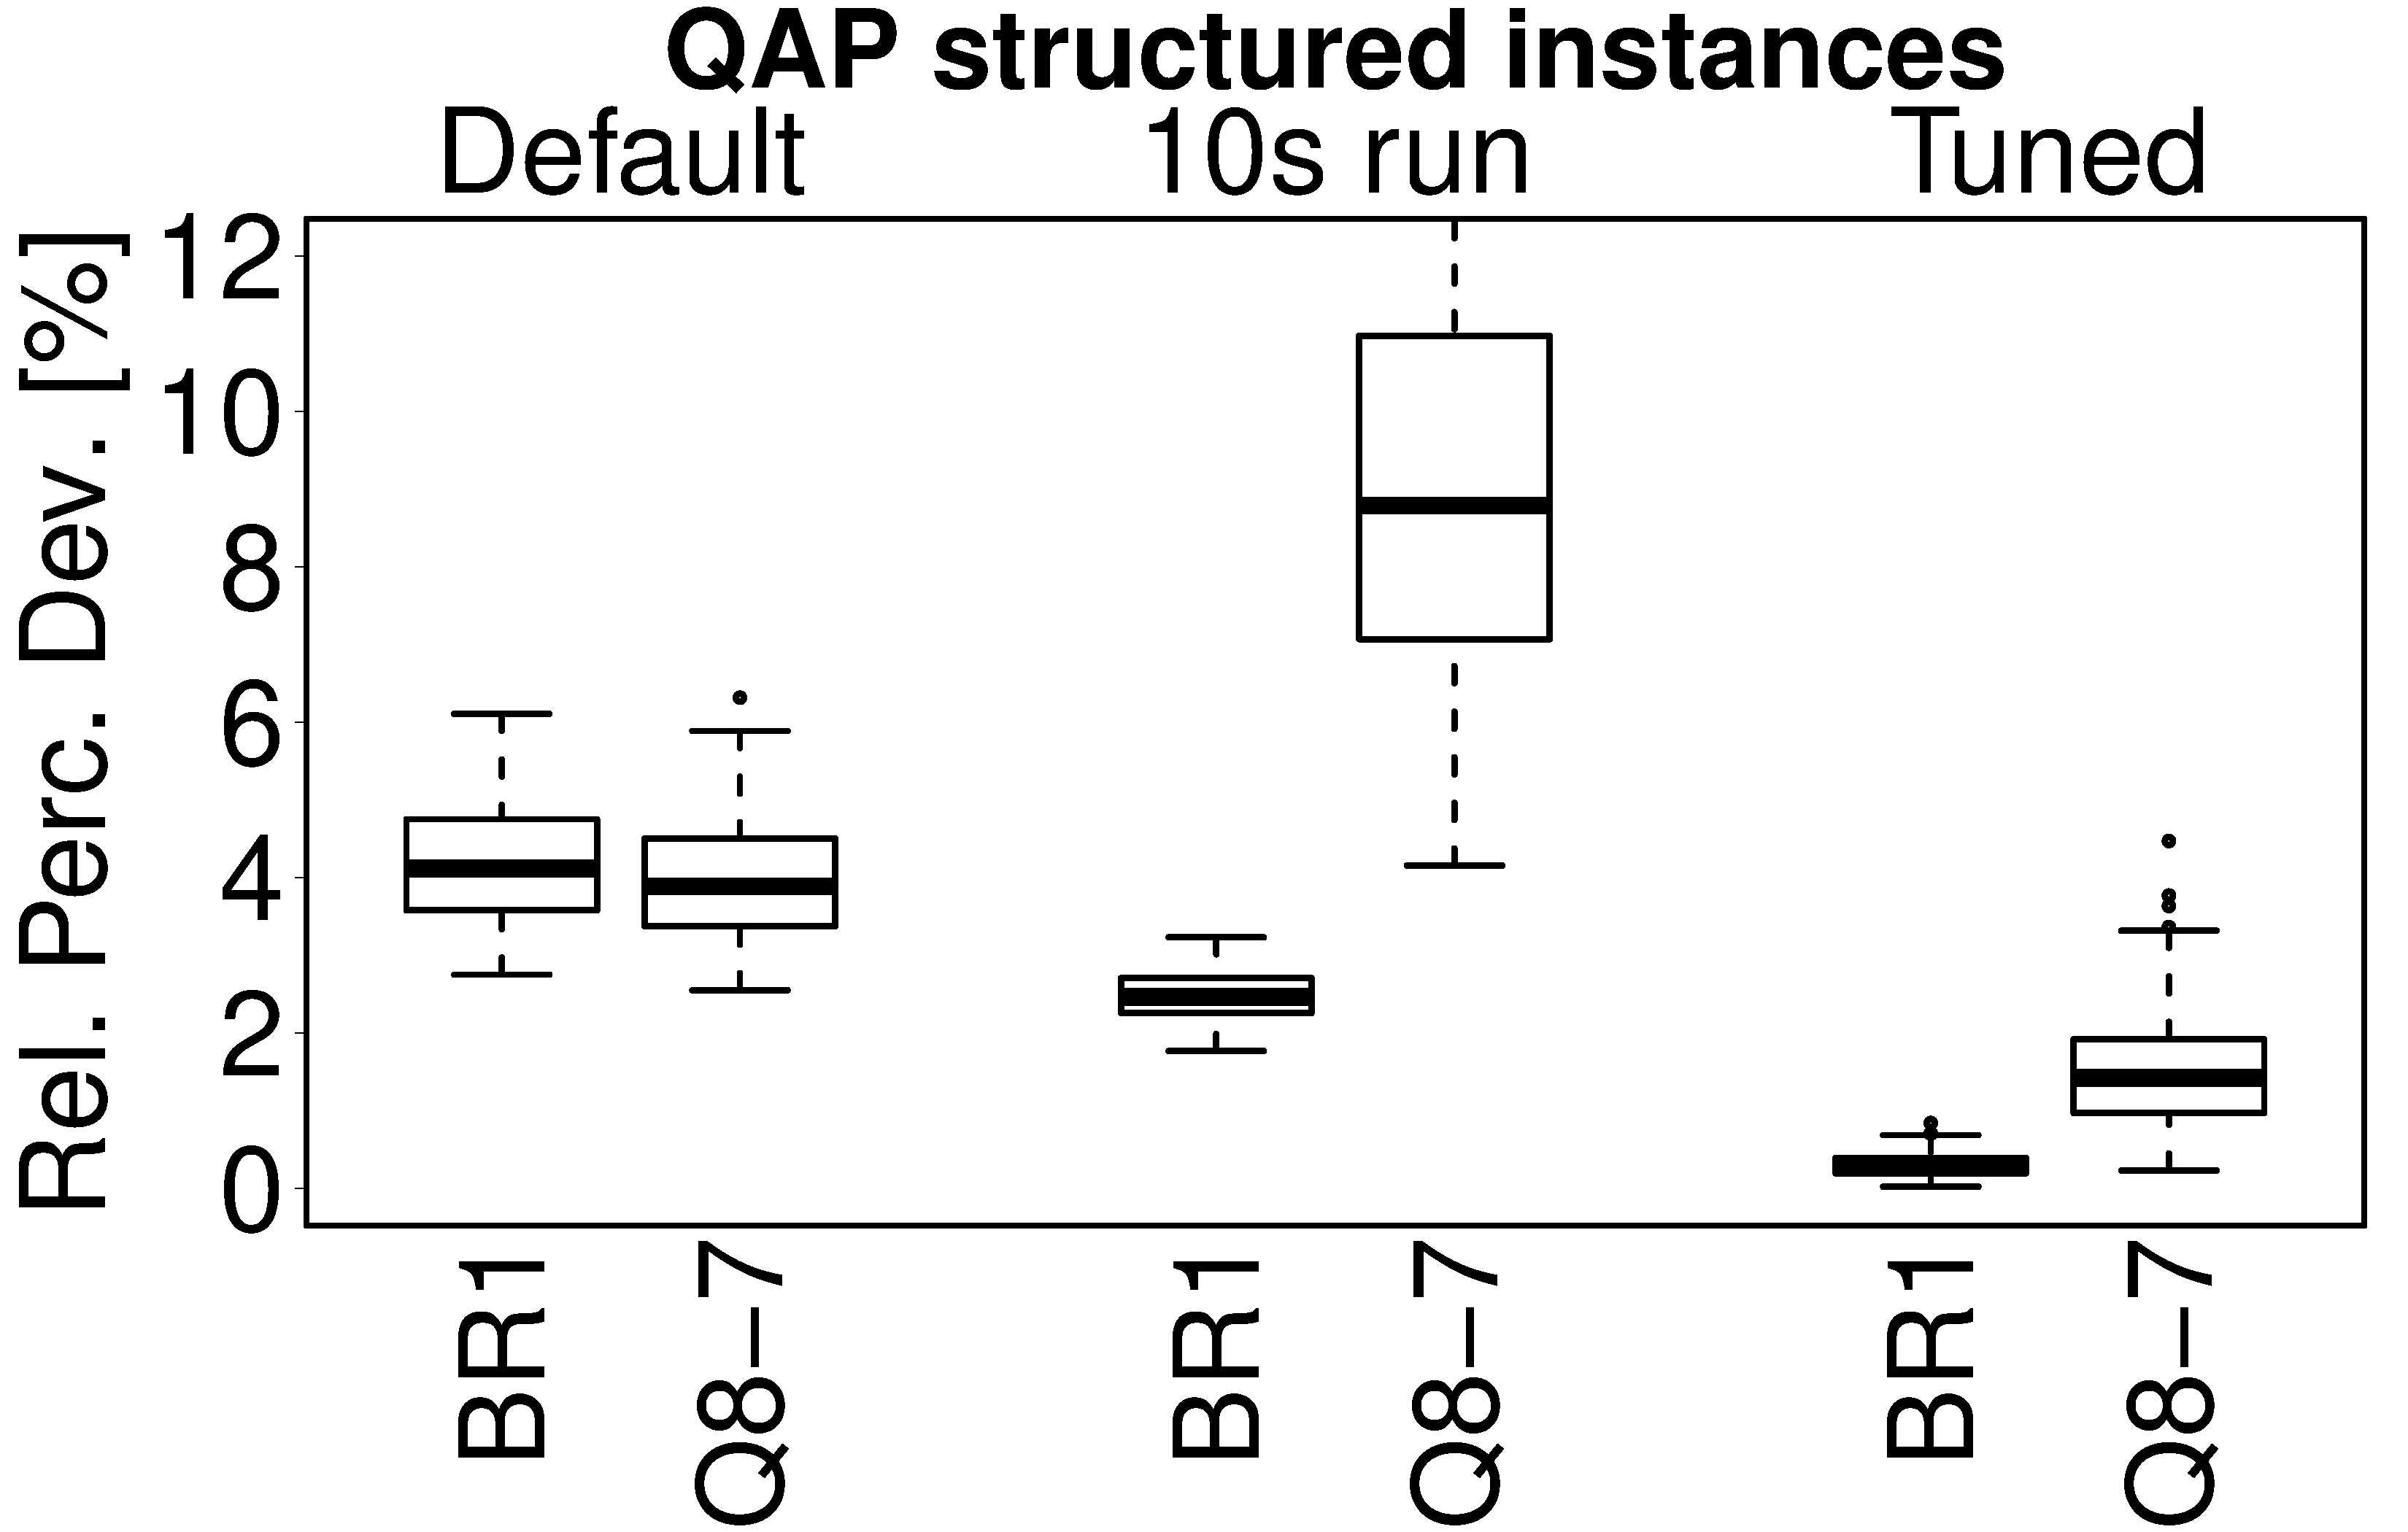
\includegraphics[width=0.49\textwidth]{Part 2 - Search-Based Optimization/Simulated Annealing/figures/es-bxp.pdf}
    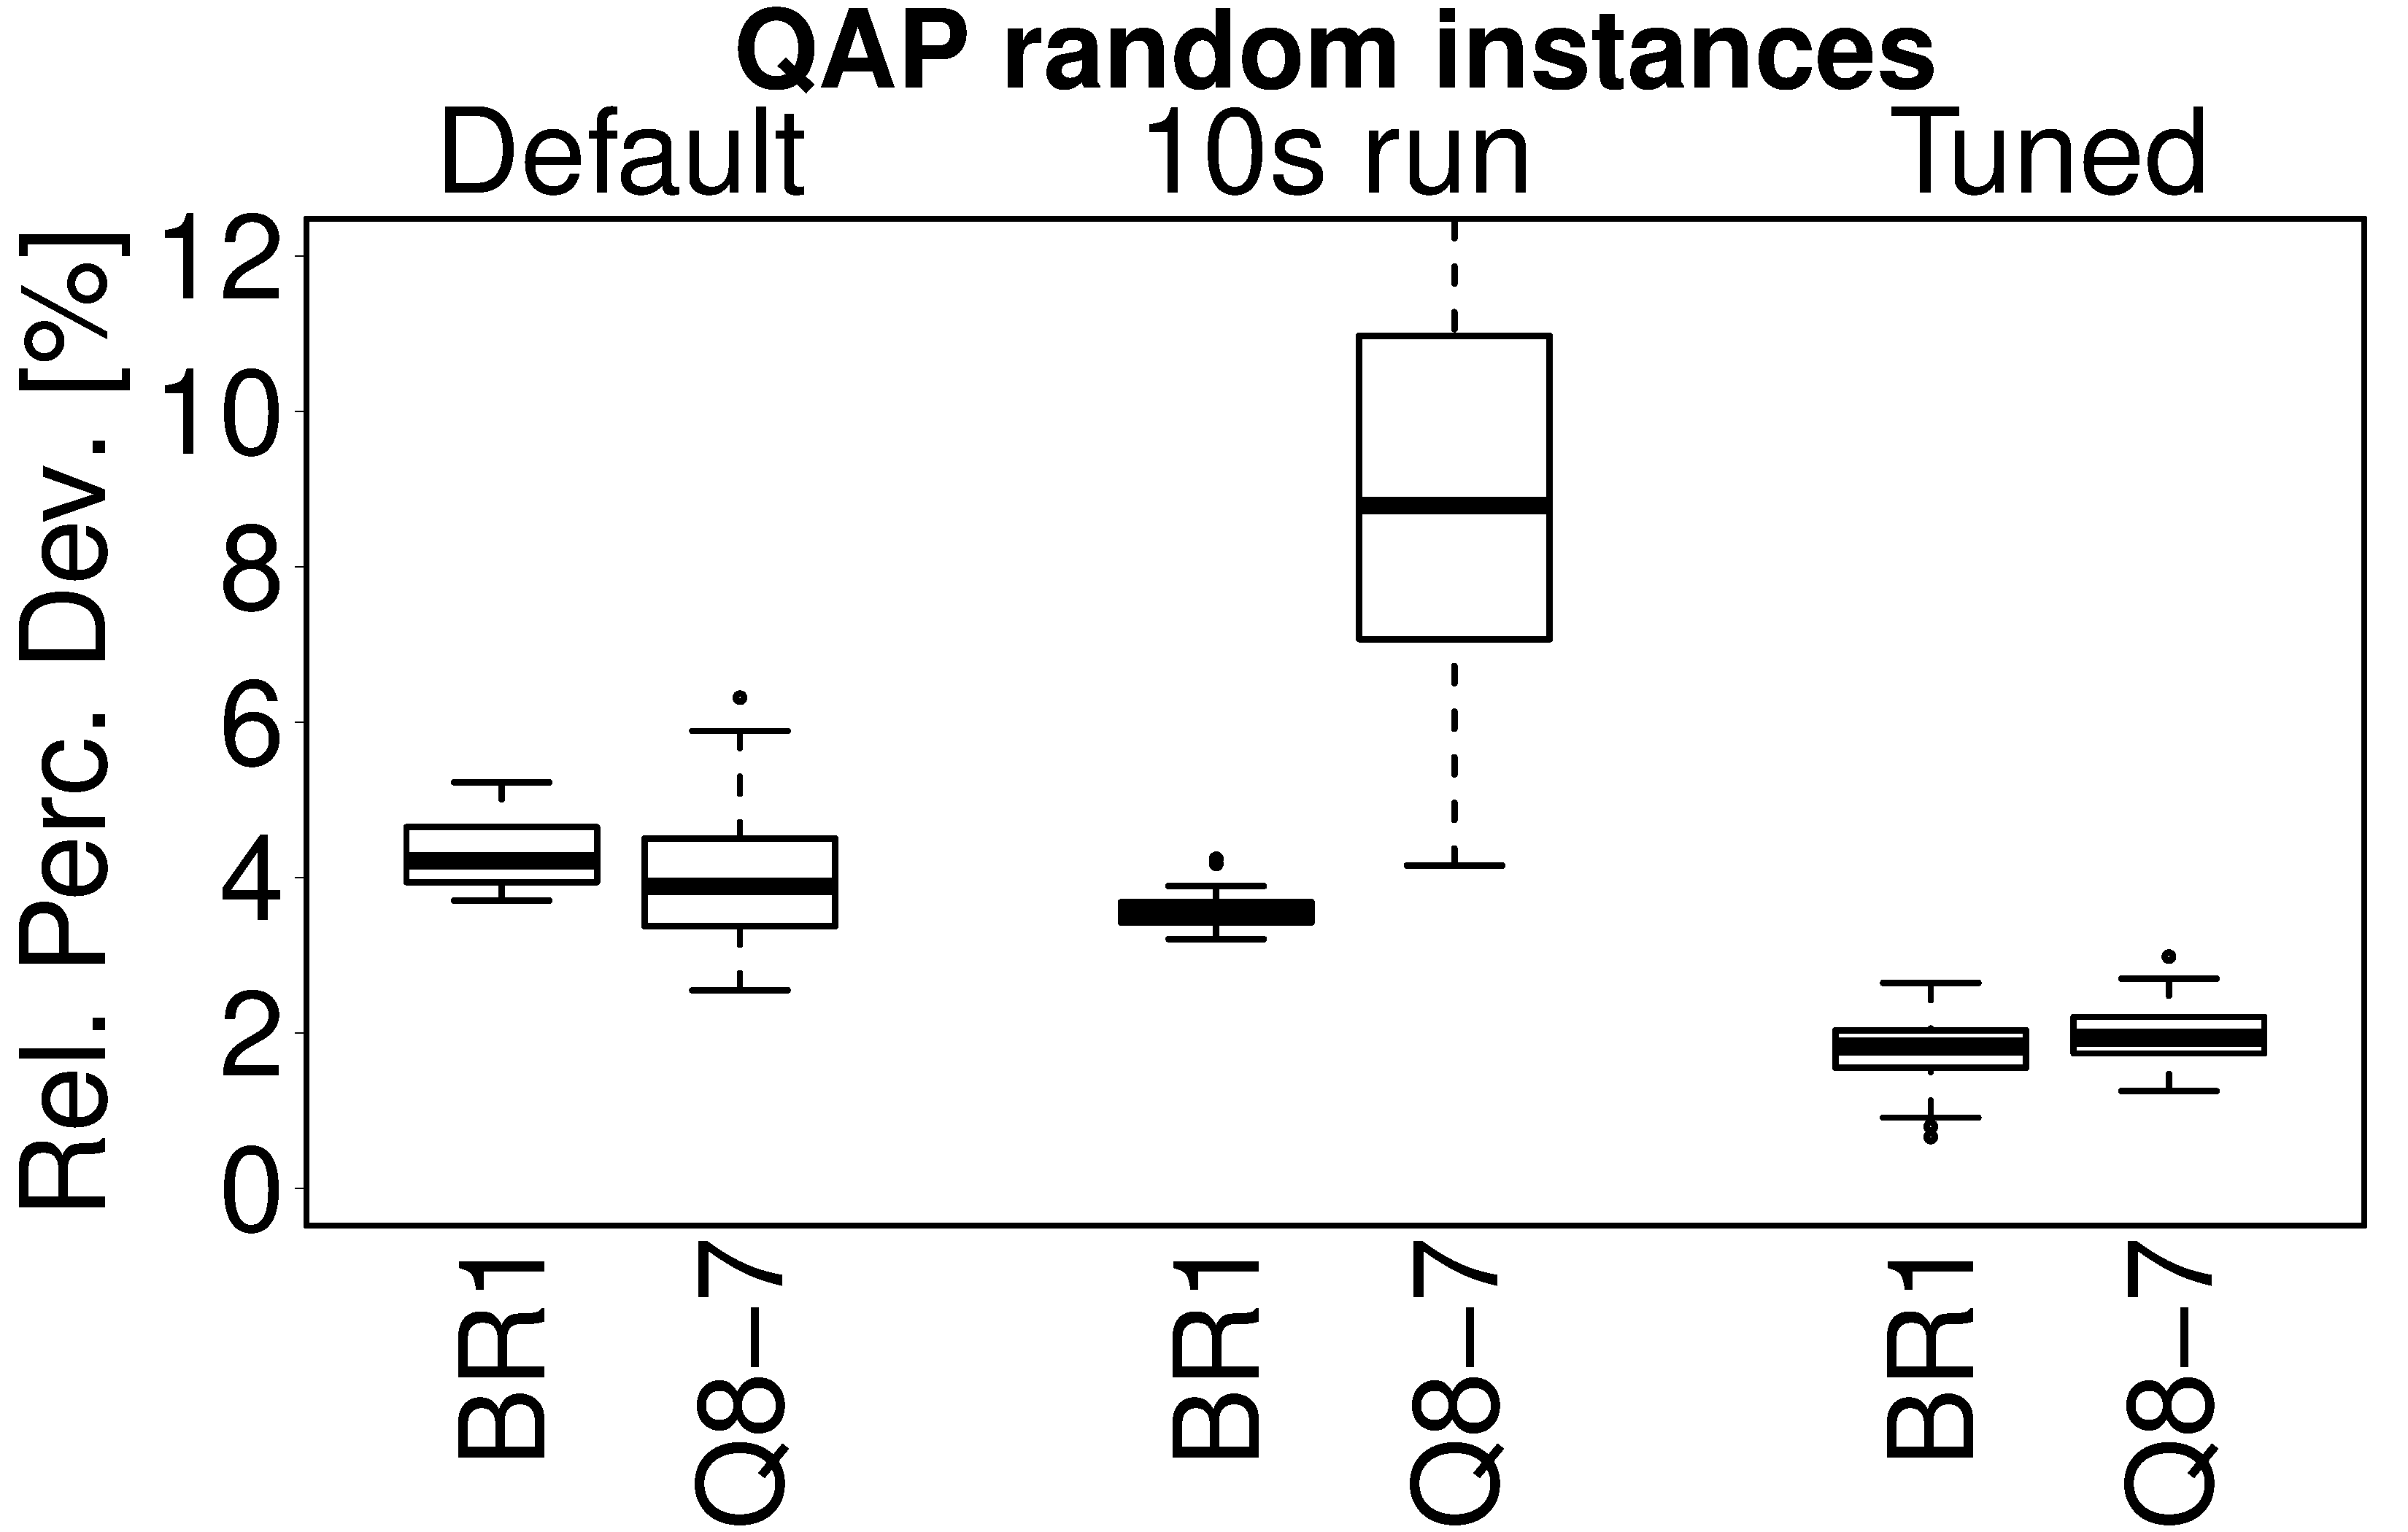
\includegraphics[width=0.49\textwidth]{Part 2 - Search-Based Optimization/Simulated Annealing/figures/rr-bxp.pdf}
  \end{center}
  \caption{Percentage deviation from the best known solutions obtained
  by the two simulated annealing algorithms on our structured
  and random QAP test set in their default settings, when let run for ten seconds,
  and when tuned using irace on a separate training set.}
  \label{fig:resqap1}
\end{figure}

In the first experiment the results obtained by \brsa and \qsa are similar, with a relative percent 
deviation (RPD) around $4\%$. This is because the algorithms are fairly old and 
most likely they have been manually
fine-tuned on small instances with little computational power available. 
If we let them run for a longer time, 
which can be done by simply replacing the termination condition,
this clearly favours \brsa that improves its results. 
The same modification has however a surprising effect on \qsa, which 
significantly worsens its results. This can be explained by considering 
how the Q8-7 cooling scheme is defined in the original paper. When 
this component is re-implemented exactly as described, one of the parameters
is computed relatively to the expected number of total move 
evaluations of the search. This value defines
therefore a delicate balance, that collapses if this value 
increases dramatically, as it is the case in our experiments. The resulting 
value makes therefore the temperature update too slow, and the algorithm
is unable to remain on good converging paths as it has a very high probability
of accepting worsening moves for a too large part of the search. 
We then tune the numerical parameters of the algorithms using irace, paying
attention to modifying the Q8-7 cooling scheme such that its parameters
can be independently configured. In this case, on both instance classes
both algorithms significantly improve their performance. 
On the structured instances, however, \brsa with an RPD of around $0.2\%$ 
clearly outperforms \qsa, which finds solutions on average worse than $1\%$ 
over the best known ones. On the random instances, instead, both algorithms obtain 
solutions on average just below $1\%$ of RPD, with \brsa marginally better than \qsa.

\begin{figure}[tb]
  \begin{center}
    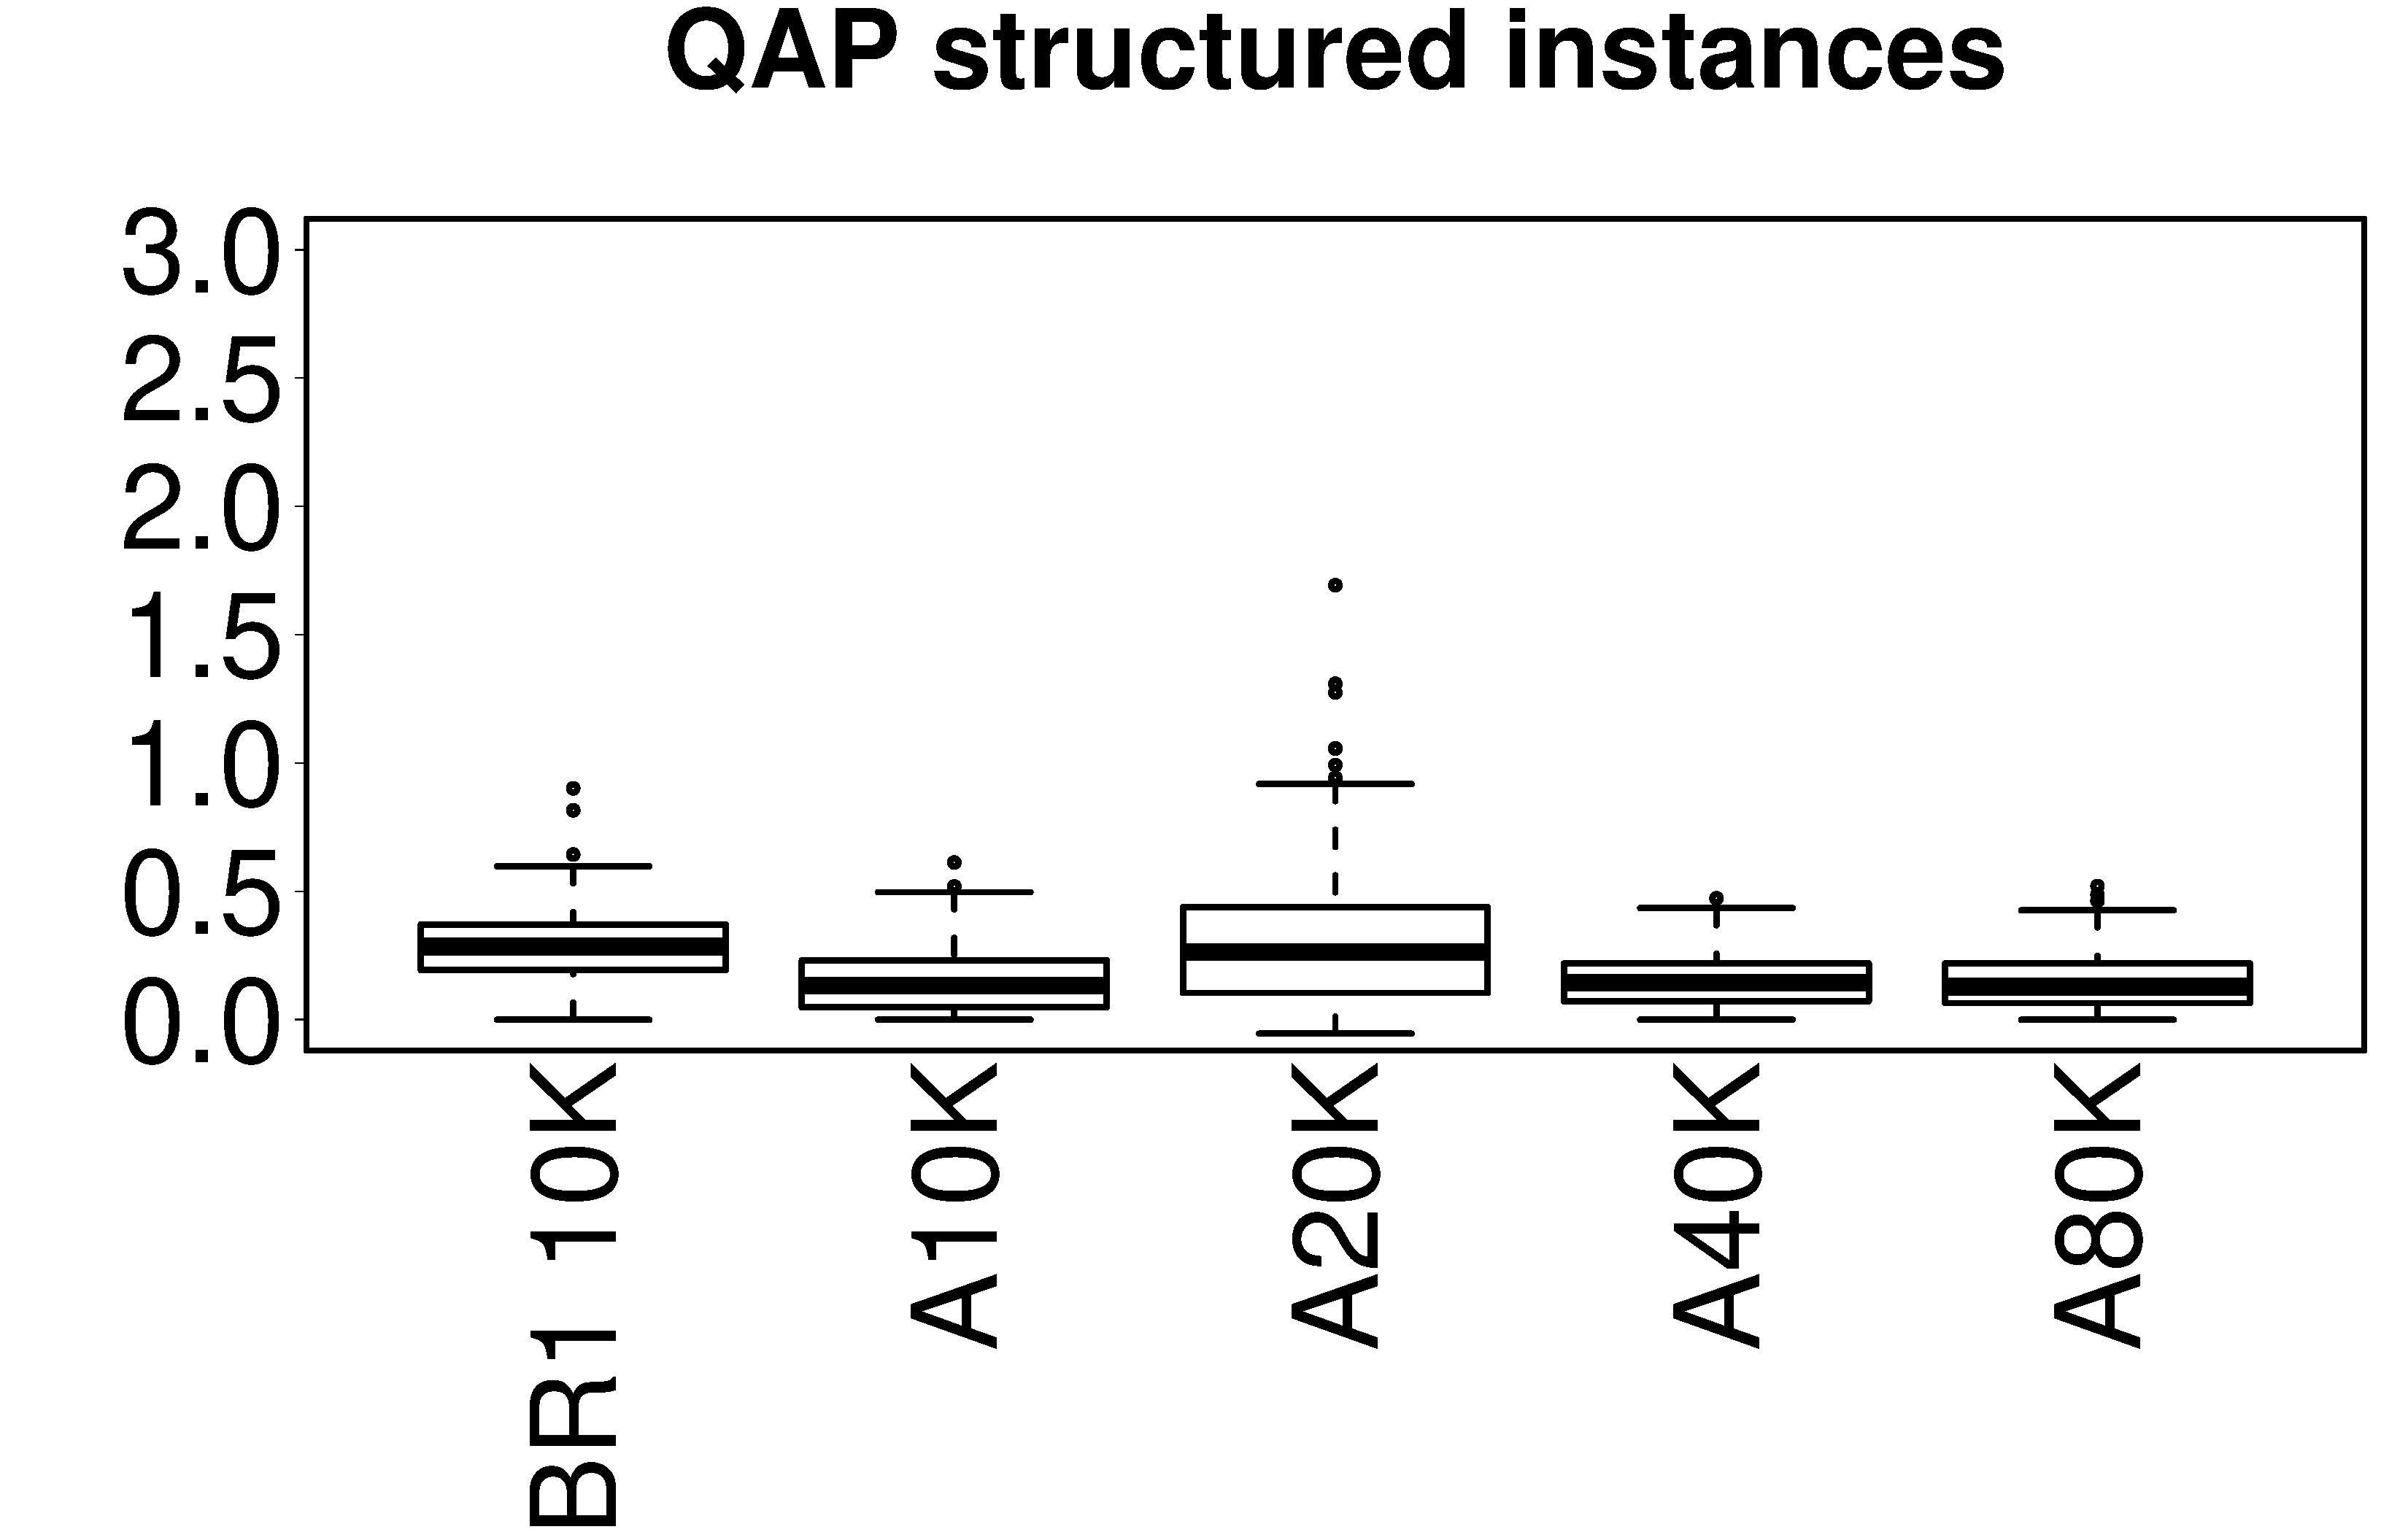
\includegraphics[width=0.49\textwidth]{Part 2 - Search-Based Optimization/Simulated Annealing/figures/esall-bxp.pdf}
    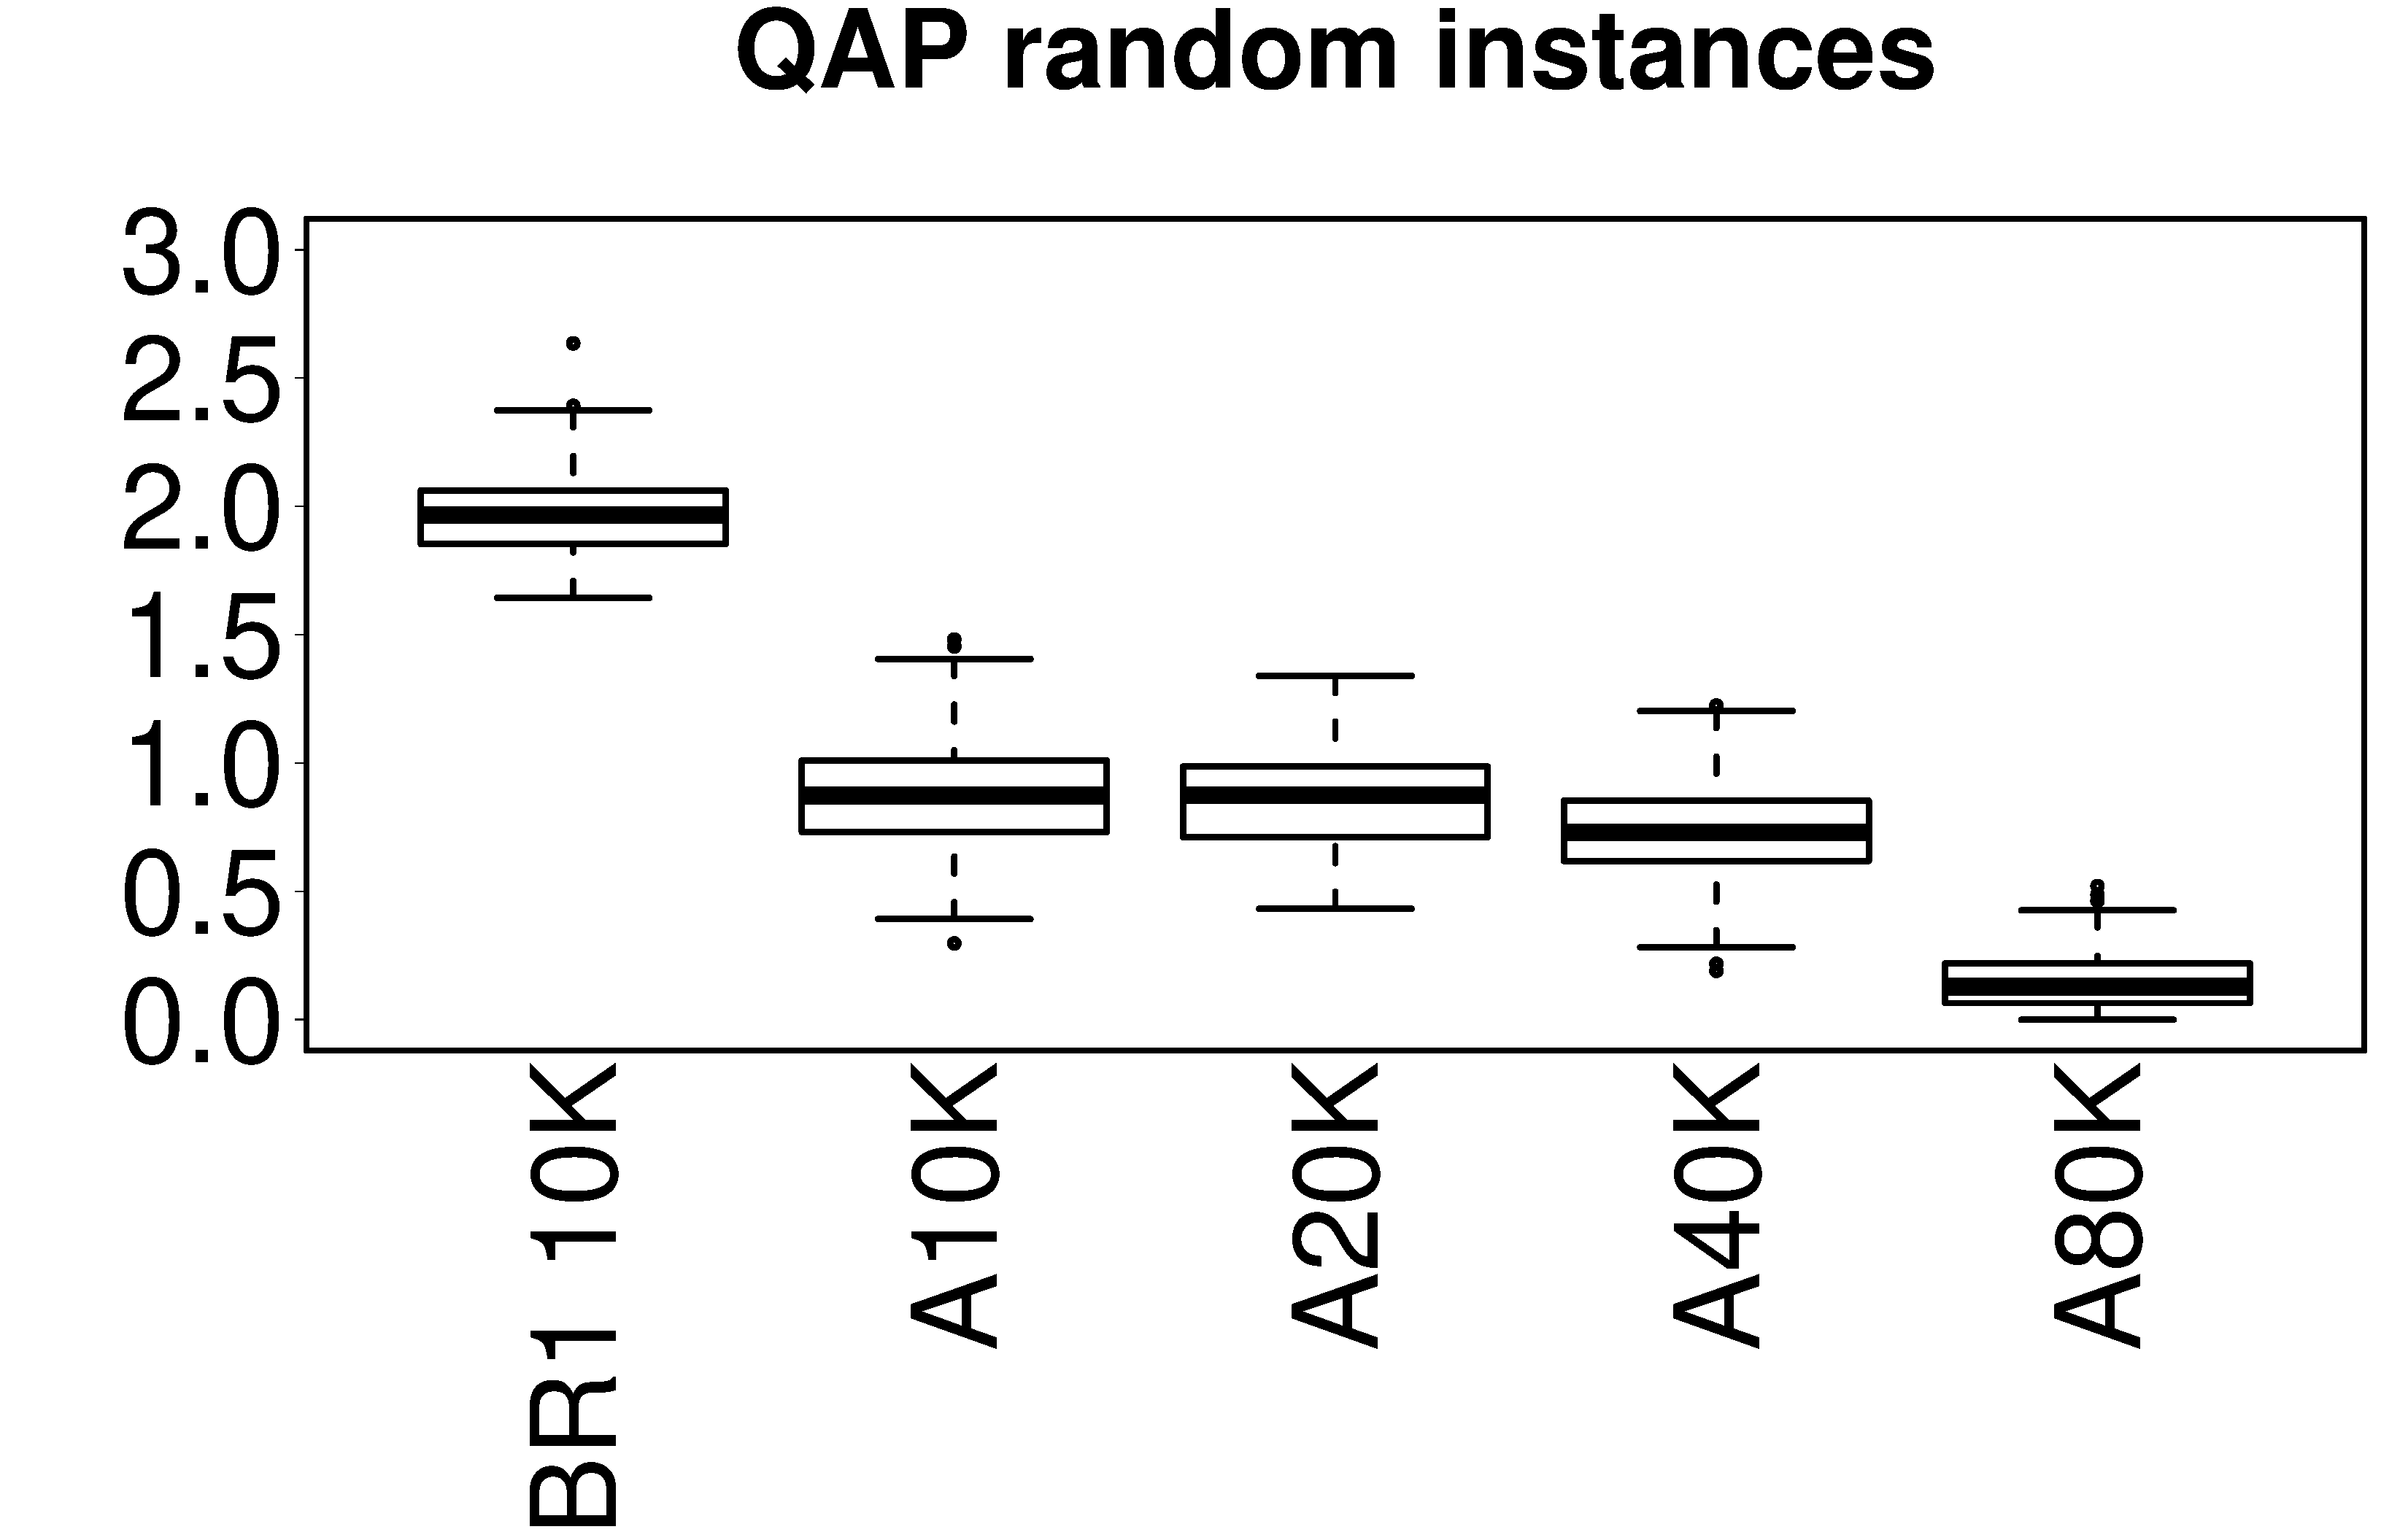
\includegraphics[width=0.49\textwidth]{Part 2 - Search-Based Optimization/Simulated Annealing/figures/rrall-bxp.pdf}
  \end{center}
  \caption{Percentage deviation from the best known solutions obtained
  when automatically designing simulated annealing algorithms from scratch using $10$K, $20$K, 
  $40$K and $80$K experiments on our structured and random QAP test set, compared
  with \brsa tuned with $10$K experiments.}
  \label{fig:res2qap}
\end{figure}


\subsubsection{Generating new algorithms}
Finally, we exploit the whole set of options identified in the literature
for the different simulated annealing components, using irace to automatically select
the best combination and thus design new algorithms from scratch. We report
in Figure \ref{fig:res2qap}
the results obtained by the algorithms that result from automated design tasks
with $10$K, $20$K, $40$K and $80$K experiments.
The algorithms obtained with the highest budget are reported 
in Algorithms \ref{algo:allsaes} and \ref{algo:allsarr} for 
structured and random instances, respectively.


\begin{algorithm}[ht!]
	  \caption{Component-based formulation of the SA automatically designed 
	  for the structured instances with a tuning budget of $80$ thousands experiments. 
	  The components are highlighted in \textit{italic}.}
     \label{algo:allsaes}
    
    Parameters: a problem instance $\mathcal{I}$, the \textit{$2$-exchange neighbourhood}, 
    \textit{a random permutation $\mathbf{x}_0$}, control parameters 
    $\theta = (p, 0.2249, k = 0.6969, \beta = 4645.392, \alpha = 0.6921, \gamma = 32)$
    
    Output: the best solution $\mathbf{x^*}$ found during the search.
    
	\begin{algorithmic}[1] 
		\STATE{$\textrm{best solution } \mathbf{x^*} := \textrm{incumbent solution } \mathbf{\hat{x}} := \mathbf{x}_0$\;}
		\STATE{$i := 0$\;}
        \STATE{Initialize temperature $T_0$ as \textit{the value that gives an expected initial acceptance probability $p$ of worsening moves in a random walk of length $l=10^4$, with a scaling factor $k$} \;}
		\WHILE{\textit{less than $10$ seconds of runtime}}
		\STATE{choose a solution $\mathbf{x}_{i+1}$ in the \textit{$2$-exchange neighbourhood} of $\mathbf{\hat{x}}$ \textit{at random}\;}
		\IF{$ \mathbf{x}_{i+1}$ meets \textit{Metropolis criterion}}
		\STATE{$ \mathbf{\hat{x}} := \mathbf{x}_{i+1}$\;}
		\IF{$ \mathbf{\hat{x}}$ improves over $\mathbf{x^*}$}
		\STATE{$\mathbf{x^*} :=  \mathbf{\hat{x}}$\;}
		\ENDIF
		\ENDIF
		\IF{\textit{the temperature value drops below} $\beta$}
		\STATE{update temperature according to \textit{geometric cooling with factor} $\alpha$\;}
		\STATE{reset temperature \textit{to initial value $\gamma$ times the neighbourhood size}\;}
		\ENDIF
		\STATE{$i := i + 1$\;}
		\ENDWHILE
        \STATE{return $\mathbf{x^*}$\;}
	\end{algorithmic}
\end{algorithm}


\begin{algorithm}[ht!]

	  \caption{Component-based formulation of the SA automatically designed for 
	  the random instances with a tuning budget of $80$ thousands experiments. 
	  The components are highlighted in \textit{italic}.}
     \label{algo:allsarr}
    
    Parameters: a problem instance $\mathcal{I}$, the \textit{$2$-exchange neighbourhood}, 
    \textit{a random permutation $\mathbf{x}_0$}, control parameters 
    $\theta = (k = 0.5438, \delta = 632, \alpha = 0.0.5927, \beta = 0.65, \gamma = 1208, r = 71822, s = 0.0828)$
    
    Output: the best solution $\mathbf{x^*}$ found during the search.
    
	\begin{algorithmic}[1] 
		\STATE{$\textrm{best solution } \mathbf{x^*} := \textrm{incumbent solution } \mathbf{\hat{x}} := \mathbf{x}_0$\;}
		\STATE{$i := 0$\;}
        \STATE{Initialize temperature $T_0$ as \textit{the average gap between consecutive solutions in a random walk of length $l=10^4$, with a scaling factor $k$} \;}
		\WHILE{\textit{less than $10$ seconds of runtime}}
		\STATE{choose a solution $\mathbf{x}_{i+1}$ in the \textit{$2$-exchange neighbourhood} of $\mathbf{\hat{x}}$ \textit{as the best one among $\delta$ randomly chosen ones}\;}
		\IF{$ \mathbf{x}_{i+1}$ meets \textit{Metropolis criterion}}
		\STATE{$ \mathbf{\hat{x}} := \mathbf{x}_{i+1}$\;}
		\IF{$ \mathbf{\hat{x}}$ improves over $\mathbf{x^*}$}
		\STATE{$\mathbf{x^*} :=  \mathbf{\hat{x}}$\;}
		\ENDIF
		\ENDIF
		\IF{\textit{exponentially increasing temperature length with parameters $r,s$} is met}
		\STATE{update temperature according to \textit{geometric cooling variant with factors} $\alpha, \beta$\;}
		\STATE{reset temperature \textit{to the one of the best solution found if no move accepted in the last $\gamma$ ones}\;}
		\ENDIF
		\STATE{$i := i + 1$\;}
		\ENDWHILE
        \STATE{return $\mathbf{x^*}$\;}
	\end{algorithmic}
\end{algorithm}

On the structured instances the results are slightly better than those obtained
by \brsa, with the exception of the configuration found with $20$K experiments.
This is a somewhat easy scenario, and it takes relatively little effort
to find good solutions. 
The random instances scenario is instead more challenging, and it takes 
more experiments to find a suitably good configuration. In fact, while
the tuning with $10$ thousand experiments improves a lot over \brsa,
it takes $40$ thousand experiments to marginally improve the results. Using
$80$ thousand experiments, however, it is possible to find configurations that
find solution qualities comparable to the structured instances case.

For different budgets, the results obtained on the structured instances
are very similar, and so are the algorithms. They all feature original simulated annealing components
such as the Metropolis acceptance, a geometric cooling scheme with cooling rates 
between $0.61$ and $0.83$ and a
random neighbourhood exploration.
There are instead different strategies for the temperature length and restart.
The initial temperature is defined in different ways, all of them relatively to 
some statistics computed during a preliminary random walk in the solution space. 
The algorithms obtained for the random instances are more different among each other.
The only common component is the Metropolis acceptance criterion. 
A closer inspection of the search trajectory reveals instead that
the algorithms effectively maintain the same or almost the same temperature value
for large portions of the search. In other words, the tuning process ends up shaping
a relatively complex algorithm that works like a very simple one. Our set of options
includes the possibility of maintaining the same temperature throughout the whole search, 
but it is more difficult to initially sample one with good settings, that has the chance of
surviving during the tuning.

The difference in the algorithms obtained can be explained with a closer
inspection to the landscapes traversed by the algorithms. On the random instances
the neighbourhoods have a distribution of solution values 
relatively similar to solutions in areas of different quality around the solution space, 
making this a scenario
that does not require variations of the algorithm parameters. On the 
structured instances, instead, neighbourhoods centered around average quality solutions
have different distributions of values than neighbourhoods around good solutions, and in this case
the flexibility of simulated annealing makes it more likely to adapt the algorithm to
the different areas of the landscape encountered \cite{IRIDIA-2021-005}.

It has to be noted that we considered only one tuning task for every budget, and
repeating each task with a different random seed may give algorithms that are different,
to a certain extent. At the same time, we have run the configuration tasks for the algorithm 
that has the full training set of 100 parameters for four different budgets. We commonly observe 
that a higher budget usually is good especially if the configuration tasks have many parameters. 
Anyway, one should observe that on the structured instances with 20K one has a relatively 
poor algorithm, 
something that can happen due to the stochasticity in the configuration process.



\section{Summary and Discussion}
\label{sec:conclusions}

In this chapter, we have seen how to implement a simulated annealing 
algorithm in terms of the design choices to make. 
We have shown how to combine the knowledge on algorithmic components 
and parameter settings  with automatic configuration tools 
to develop efficient simulated annealing
algorithms. This methodology is nonetheless general, 
and works for any stochastic local search method.
There are some inherent advantages 
for this such as making these components and parameters available for 
future use, allowing experimental analyses to identify the circumstances under which
every component will be most successful,
and exploiting directly the recent advances in the automatic 
configuration of algorithms.
This applies even more strongly when we want to design an algorithm that finds
good solutions as soon as possible, or, in other words, that exhibits a good 
\textit{anytime behaviour}. 

In the experiments we observed how good simulated annealing algorithms look 
like for different QAP instance classes.  
In general, in \cite{FraStu2019:cor} we have many more simulated annealing algorithms 
for the QAP identified and, independent of which simulated annealing we have, 
we found the automated configured simulated annealing with the variety of our settings 
always superior to these specifically designed algorithm for the QAP.
An importance analysis conducted across different problems and instance classes
indicated in fact that the acceptance criterion is the most important component in a
simulated annealing, followed by the neighbourhood exploration criterion. 
These two components are precisely the ones that operate locally in the neighbourhood.
In general, we have seen that different scenarios require different algorithms,
but even for the same scenario we may have different algorithms that perform 
equally well. 
Quantifying the appropriate diversification and understanding what algorithm 
could obtain the desired behaviour are anyway tasks 
better performed with the help of automatic tools. They can, in fact, 
select the best options for each algorithmic component and parameter, 
thus making the best out of the available body of knowledge that can be
found in the literature. 

A different approach is extending our approach to other stochastic local search methods and to 
generate extended frameworks. Ideally, these extensions would be 
generated within a same framework so that possibly rich hybrids 
among these methods may be generated. This would enable us to 
compare automatically designed simulated annealings against other automatically 
designed stochastic local searches, to study the role, impact and composition of 
simulated annealing algorithms when combined with or used as part of other 
stochastic local searches. Ultimately, we can try to understand 
when and how to move beyond the simulated 
annealing structure, to automatically design bottom up new methods without 
constraining them to a predetermined form.

\section{Exercise}\label{sec:exercise}
In addition to \brsa and \qsa, in the literature there are several papers
proposing SA algorithms for the QAP or for problems that can be modeled
as such. 
We propose an open-ended exercise to become acquainted not only with 
Simulated Annealing, but also with a component-based perspective
on stochastic local search algorithms, and its automatic optimization.
You can take inspiration from the Supplementary Material of this chapter\footnote{\supplementurlsa}, but you can also start with a new clean implementation.

\begin{enumerate}
    \item Choose a SA for the QAP to implement. You can start from the works we
    cited in this Chapter, or you can look for other SA algorithms.
    \item Identify the components of the algorithm you chose
    comparing it with against the template we provide in Section
    \ref{sec:sacomponents}, along with their numerical parameters.
    \item Understand how they interact: think about each of them as a separate
    function, and analyze which data can be considered \textit{input}
    and \textit{output}.
    Use the template given in Algorithm \ref{algo:simannealing} as a  
    reference to determine the flow of information among the components.
    \item Implement the algorithm, making sure you can specify the 
    numerical values as command line parameters. SA is
    a stochastic algorithm, so remember to
    make it possible to specify a random seed too.
    \item Run some tests on the instances we provide in the Supplementary
    Material\footnote{\supplementurlsa}. Use different random seeds and record the results
    you observe.
    \item Play with the numerical parameters, trying to find
    a parameter combination that performs consistently better than
    the original parameter values.
    \item Use irace and the templates
    provided in the Supplementary Material\footnote{\supplementurlsa} to automatically tune
    the numerical parameters \cite{LopDubPerStuBir2016irace}. 
    Re-run the tests, and observe the difference of results.
    \item If you feel brave, implement alternative components, such as
    new functions to update the temperature value, or to determine 
    whether to accept a candidate solution. You can take these ideas
    from existing papers, or come up with new components on your own.
    An implementation that reflects the component-based perspective
    of SA will make it way easier to observe the impact of your new
    components. You can even introduce a new command line parameter
    to add the choice at runtime.
\end{enumerate}

\section*{Acknowledgments}
Alberto Franzin acknowledges support from the 
Service Public de Wallonie Recherche under grant n\textdegree 2010235 - ARIAC by DIGITALWALLONIA4.AI.
Thomas St\"utzle acknowledges support from the Belgian F.R.S.-FNRS,
of which he is a Research Director. 

\bibliographystyle{unsrt}
\bibliography{bibliography}

\title{Differential Evolution}
\label{chp:differential-evolution}
\author{}
\institute{}
\maketitle


Add your content here


\bibliographystyle{unsrt}
\bibliography{bibliography}

\title{Particle Swarm Optimization}
\label{chp:particle-swarm-optimization}
\author{Diego Oliva, Alfonso Ramos-Michel, Mario A. Navarro, Eduardo H. Haro, Angel Casas}
\institute{Universidad de Guadalajara, CUCEI}
\maketitle

%\textbf{Abstract}\\
%Particle swarm optimization (PSO) is one of the most important meta-heuristic algorithms. It serves as a base for modern methods and has been applied in several fields. Its importance is due to its simplicity and collective behavior that permits finding the optimal solutions to complex problems. The popularity of the PSO also permits researchers to design different variants that improve its performance. This chapter analyzes the importance of the PSO as an intelligent algorithm. Here are presented the basic concepts of the PSO, some examples, and a study of the most important variants and applications. The idea is to provide the reader with an overview of this interesting approach.


%This file lists some brief information about how optimization problems are going to be defined in the IEEE CIS Open Book. We ask your book sections to follow the notations listed here for consistency. If you have any questions regarding the notation, please contact Leandro Minku (l.l.minku@bham.ac.uk). 

%Please use the svmult style file and follow Springer's svmult guidelines, which can be downloaded here: \url{https://www.springer.com/birkhauser/mathematics?SGWID=0-40292-2-122598-0}. Please use the ruled and graybox options of the style file.

%Section \ref{sec:intro} presents the notation for machine learning. Section \ref{sec:optimization} presents the notation and some definitions for optimization. Section \ref{sec:alg} presents the notation for pseudocode. Example citations are as follows: \cite{KocaguneliEtAl2013}, \cite{KocaguneliEtAl2013-2}.

%We also ask authors to adopt American spelling for the English language used in the sections, if possible. 


%\hfill
%\section{Introduction}
%\label{sec:intro}

Nature is the source of inspiration for different processes in science and engineering. Since nature is an example of the world, humans have tried to imitate different behaviors over the years. This occurs not only in a personal way but also happens in the creations and constructions. The collective behavior that is present in an animal that lives in groups is a clear example of how nature solves the problem of finding sources of food, shelters, or places to migrate. In the case of food sources or hunting, a group is more capable of finding food than a single animal. This means that with more members of the group have more probability of catching prey. 

In computer sciences, intelligent algorithms' design could be seen as an attempt to imitate nature. In this sense, techniques such as Particle Swarm Optimization (PSO) is an example of inspiration from nature as a base to solve complex problems \cite{kennedy1995particle}. The PSO is part of a group of methods called meta-heuristic algorithms that are widely important in artificial intelligence and applied mathematics. Meta-heuristic algorithms can use a biological, physical, or social phenomenon as a source of inspiration and provide the basis for modeling operators to perform optimization.

The PSO was initially proposed by Kennedy and Eberhart in 1995. It was developed to simulate the unpredictable choreography of birds flocking, but later it was used to solve many problems defined discrete-valued spaces where the domain of the variables is infinite \cite{kennedy1995particle}. Nonetheless, particle swarm optimization has attracted the scientific attention of miscellaneous engineering and physics areas; this is because there are several fields of study where it is necessary to find better solutions according to specific established criteria. Some other classical optimization approaches cannot be used in these types of problems because they could get caught in local optima \cite{janeza2009pso}. Even though particle swarm optimization has some similarities with genetic algorithms and other optimization approaches, the main difference is that instead of using mutation/crossover operators, it uses the global communication and real-number randomness as the swarm particles \cite{yang2010nature}.

The PSO works with a population of candidate solutions that are called particles. Each particle of the population collaborates with its search strategy to improve the quality of the solutions. In the early research related to PSO, we can see that the operators move the population as birds flock or school of fishes. PSO is then a simple optimization algorithm that allows to explore a search space and find the optimal solution. Due to its simplicity, PSO is a popular method, and it has been applied in different domains, from benchmark optimization problems to medical applications \cite{shi2001particle}. PSO has been studied by researchers over the years not only to use it for solving complex problems but also to understand how this algorithm works and to validate its performance from theoretical and empirical points of view \cite{shi1999empirical}. PSO is considered a powerful tool for optimization, and it is a classical approach that helps to inspire other algorithms such as swarm intelligence \cite{eberhart2001swarm}. However, PSO, like many other algorithms, has some drawbacks; for example, it could be trapped in sub-optimal solutions in complex search spaces (multi-modal problems). In this sense, in the related literature, they are more than 100 modifications of the PSO, and their modification is still growing every year \cite{imran2013overview}.

The popularity of PSO is reflected in the number of cites and publications indexed in different databases like Scopus. Figure~\ref{fig:PSOyear} shows a plot extracted from Scopus related to PSO from 2010 to 2021. From this graph, it is possible to see that in 2010 they were around 4000 documents published, and in 2020 the number of publications was between 8000 and 9000.

\begin{figure}[h!]
  %\vspace*{-.2cm}
  \centering
  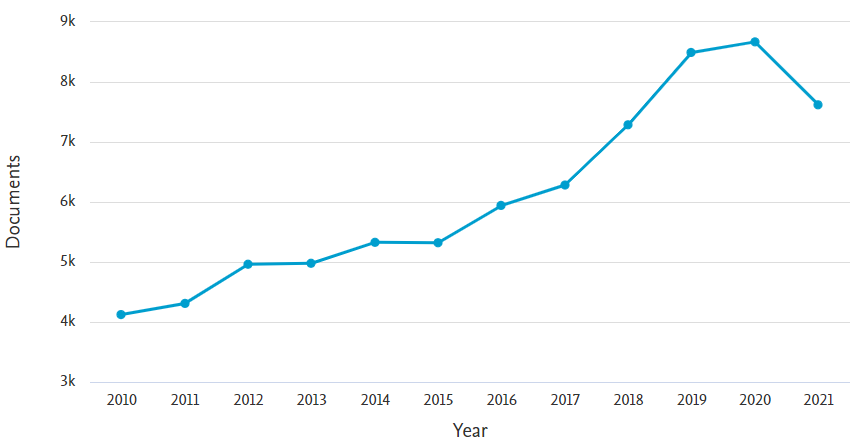
\includegraphics[scale=0.5]{"Part 2 - Search-Based Optimization/Particle Swarm Optimization/Images/PSO Year.PNG"}
  %%\vspace*{-.4cm}
  \caption{Number of articles per year of PSO between 2010 and 2021. \label{fig:PSOyear}}
  %\vspace*{-.3cm}
\end{figure}


%The modifications of PSO are also part of this case in the computer science or engineering field. 
To graphically show where the PSO impacts in the last ten years Fig.~\ref{fig:PSOarea}  presents a pie chart. The main field of application is engineering, followed by computer sciences, and third place in mathematics.

\begin{figure}[h!]
  %\vspace*{-.2cm}
  \centering
  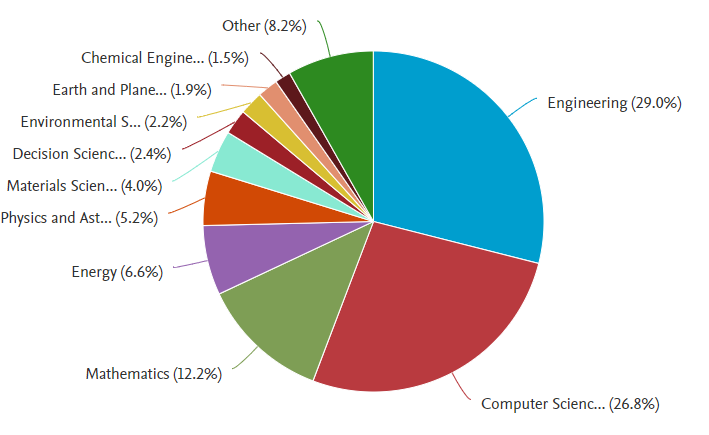
\includegraphics[scale=0.5]{"Part 2 - Search-Based Optimization/Particle Swarm Optimization/Images/PSO Area.PNG"}
  %%\vspace*{-.4cm}
  \caption{Documents by subject area related to PSO between 2010 and 2021. \label{fig:PSOarea}}
  %\vspace*{-.3cm}
\end{figure}

In this chapter, an introduction to the PSO algorithm is given. The goal is to provide an overview of the PSO, explain its basic concepts and operators, and present examples and exercises. Besides, the variants of the PSO are also discussed based on their importance in the scientific community. In the same context, they also studied the most important application of this vital algorithm.

The rest of the chapter is organized as follows: Section \ref{sec:psobasics} explains the operators of the PSO. Section \ref{sec:variants} discusses the main modification of the PSO. In Section \ref{sec:apps} are analyzed the most important PSO applications. Finally, Section \ref{sec:conclusions} discuses some conclusions and proposes some exercises.
%\todo[inline]{ DIEGO}
%Supervised learning: consider a set of examples 

%\[\mathcal{T} = \{(\mathbf{x}^{(1)},y^{(1)}),(\mathbf{x}^{(2)},y^{(2)}),\cdots,(\mathbf{x}^{(N)},y^{(N)})\}\]

%\noindent where $(\mathbf{x}^{(i)},y^{(i)}) \in \mathcal{X} \times \mathcal{Y}$  are drawn i.i.d. (independently and identically distributed) from a fixed albeit unknown joint probability distribution $p(\mathbf{x},y)$.

%Supervised learning aims at building a (predictive) model able to generalise to unseen (test) examples of the same probability distribution $p(\mathbf{x},y)$. In classification problems, $\mathcal{Y}$ is a set of categories / classes. In regression problems, $\mathcal{Y}$ is $\mathbb{R}$.

%Supervised learning aims at learn a (predictive) model able to generalise to unseen (test) examples of the same probability distribution% $p(\mathbf{x},y)$. In classification problems, $\mathcal{Y}$ %is a set of categories / classes. In regression problems, $\mathcal{Y}$ is $\mathbb{​R}$.


%Mathematical notations:
%\begin{itemize}
%\item Scalar: lower case, e.g., $a$, $b$.
%\item Column vector: lower case, bold, e.g., $\textbf{x}$.
%\item Vector element: lower case with subscript, e.g., $x_1$, $x_2$.
%\item Matrix: upper case, bold, e.g., $\textbf{X}$.
%\item Matrix element: upper case with subscripts, e.g., $X_{1,2}$.
%\item If enumerating these (e.g., having multiple vectors), superscript will be used to differentiate this from indices, e.g., $\textbf{x}^{(1)}$, $\textbf{x}^{(2)}$.
%\item Use mathcal font for sets, e.g., $\mathcal{T}$ for training set.
%\end{itemize}

%Terms to be adopted:
%\begin{itemize}
%\item Please use the term ``input variable'' instead of ``independent variable'' or ``input attribute''.
%\item Please use the term ``output variable'' instead of ``dependent variable'' or ``output attribute''.
%\item Please use the term ``example'' instead of ``observation'', ``data point'' or ``instance''.
%\end{itemize}
 

%\newpage
\section{The fundamentals of PSO algorithm}
\label{sec:psobasics}

This section introduces the basic concepts of the standard PSO and how it works. The pseudocode is described easily, and an example permits an analysis of the behavior of the algorithm.

\subsection{The PSO structure}

Essentially, each particle in the swarm (which is considered a candidate solution) is randomly distributed and represented by a vector in a multidimensional search space; all this set of particles is considered the initial population. Once established the initial population, PSO searches for optima by updating each particle according to notions such as position, velocity, inertia, etc. These notions can be defined as a vector usually called \textit{the velocity vector}, which helps to determine the next movement of the particle. Nonetheless, this movement is not entirely random; each particle is attracted towards both its own personal best position and the best position of the swarm. Then, the population is evaluated in the objective function to determine the population quality. This also allows finding the best element that will be defined as a criterion to beat in the subsequent evaluation. The new generated positions of the particles and the speed with which they are moving are calculated considering the value of the best global element and the actual value of every particle compared with a random number \cite{erick2021matlab}.\\

When the population is initialized and evaluated, the particle with the lowest or highest objective value is obtained depending on whether it is a minimization or maximization problem, respectively. This found particle is called \textit{the global particle} $gB$. On the other hand, in each iteration of the algorithm, the current particle is compared with the newly generated particle; in other words, particles have to be evaluated in the objective function every time they are moved. If the generated particle is better than the current one, then it is replaced by the new particle, receiving the usual name of \textit{the actual best particle} $lB$. The general pseudocode of the particle swarm optimization algorithm is shown in Algorithm~\ref{alg:PSO}. In contrast, the phases of initialization and movement of particles that compose the PSO are explained in the following two subsections.\\

In order to better understand the pseudocode shown in Algorithm~\ref{alg:PSO}, it is enough to appreciate that it is divided into two main parts, the unnumbered part and the numbered part. The unnumbered part refers to those terms that the algorithm requires in order to perform its operation, terms such as the population number, dimensions, etc. Once the previous points have been established, the numbered part is given, which begins with the initialization of the population and its respective evaluation. The terms ``repeat" and ``until" refer to the beginning and end of the while loop, which is the main body of the algorithm.

\begin{algorithm}[h!]
\caption{Particle swarm optimization pseudocode}
Parameters $\rightarrow$ Dimensions, Bounds, Maximum iteration number, Number of particles.\\
Output $\rightarrow gB$.   
\begin{algorithmic}[1]
\STATE{Initialize the particles of population.}
\STATE{Evaluate the objective function.}
\REPEAT
\FOR{All particles in all dimensions}

\STATE Generate a new velocity.
\STATE Calculate a new position.
\STATE Evaluate again the objective function.
\ENDFOR
		
\STATE Update the best particle of population.
\UNTIL the maximum number of iterations is reached.
\end{algorithmic}
\label{alg:PSO}
\end{algorithm}

\subsubsection{Initialization of the PSO}

All meta-heuristic algorithms have an initialization phase that has the primary purpose of creating the initial population, where each particle represents a candidate solution for the optimization problem. These particles are randomly generated in a search space, which is delimited by the established bounds. Generally, the initialization phase also defines the parameters of the problem to optimize \cite{erick2021matlab}. The initialization of the PSO algorithm is defined by Eq.~\ref{eq:equation1}, which describes the optimization of its individual particles.

\begin{equation}
\vec{x}_{i,j}^t=lb_j+rand(ub_j-lb_j)
\label{eq:equation1}
\end{equation}

\noindent where $\vec{x}_{i,j}^t$ is the $i-th$ population particle, $i \in \{i=1,2,3,...,N\}$ represents the index of a given particle, $N$ is the maximum number of particles, $j$ represents the $j_{th}$ dimension of the design variable, where $0<j\leq d$ and $d$ is the dimensionality of the design variable. The iteration number is represented by $t$. While $lb_j$ and $ub_j$ define the lowest and upper limit, respectively. It is worth saying that $rand$ is a uniformly distributed random number between $0$ and $1$. Once established the respective position of each particle, it is necessary to define the velocity each one of them will move around the search space to find the global optimal. We will explain that phase next.

\subsubsection{Velocity and movement of particles}

To find the velocity, it is necessary to get the best global and local values of each particle, commonly called $\vec{gB}^t$ and $\vec{lB}_i^t$ respectively. Eq.~\ref{eq:equation2} defines the velocity calculation for each particle $i$:

\begin{equation}
\vec{v}_i^{t+1}=w \times \vec{v}_i^{t}+c_{1} \times \vec{r1}_i^t \times (\vec{lB}_i^t-\vec{x}^{t}_i)+c_{2} \times \vec{r2}_i^t \times (\vec{gB}^t-\vec{x}^{t}_i)
\label{eq:equation2}
\end{equation}

\begin{equation}
\vec{x}_i^{t+1}=\vec{x}_i^{t}+\vec{v}_i^{t+1}
\label{eq:equation3}
\end{equation}

\noindent where $\vec{v}_i^{t+1}$ is the particle $i$'s velocity of the iteration $t+1$, $\vec{v}_i^{t}$ is the particle $i$'s velocity in the previous iteration, the vector that contains each particle $i$'s position is $\vec{x}_i^{t}$ and $\vec{r1}_i^t$ and $\vec{r2}_i^t$ represent $d$-dimensional vectors containing uniformly distributed random numbers between $0$ and $1$. It is worth to say that $c_{1}$ and $c_{2}$ are called learning coefficients, and $w$ represents an inertia weight that affects the convergence and exploration-exploitation trade-off in PSO process. Since inception of inertia Weight in PSO, a large number of variations of Inertia Weight strategy have been proposed, nonetheless, it is generally established as 1. Meanwhile, Eq.~\ref{eq:equation3} is used to displace the particles to new positions in the next iteration. Where $\vec{x}_i^{t+1}$ is the vector where the new obtained position of particle $i$ at iteration $t+1$ is stored, $\vec{x}_i^{t}$ corresponds to the previous position of particle $i$ calculated at iteration $t$, and finally $\vec{v}_i^{t+1}$ is the velocity vector obtained by Eq.~\ref{eq:equation2}.

It is essential to mention that the majority of modifications to the PSO algorithm have as purpose to find new ways to accelerate the particles as best as possible \cite{erick2016optimizacion}. To end this section, Fig.~\ref{fig:PSOmovement} shows a graphic description of particle's velocity and their movement in the particle swarm optimization algorithm for a better understanding by the reader.\\

\begin{figure}[h!]
\centering
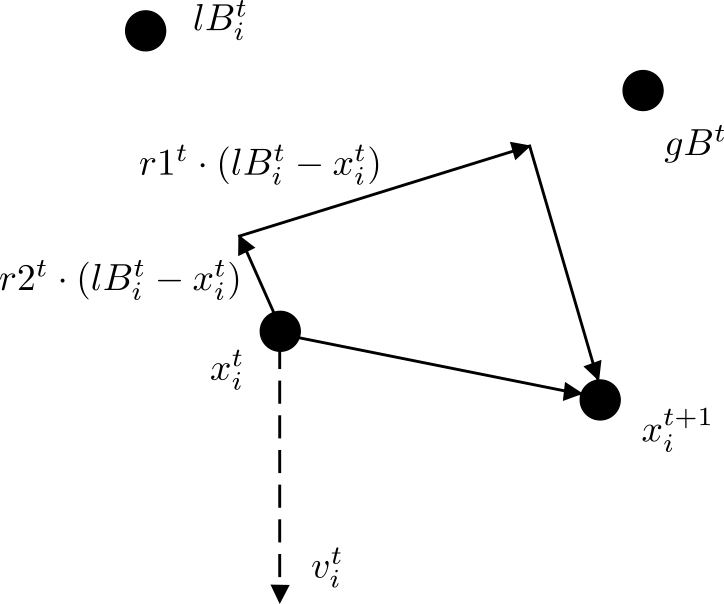
\includegraphics[scale=0.4]{"Part 2 - Search-Based Optimization/Particle Swarm Optimization/Images/Fig.1.3.png"}
\caption{Velocity and movement of particles in PSO.}
\label{fig:PSOmovement}
\end{figure}

\subsection{A PSO example}

To show how the PSO works here is presented a graphical example. Figure~\ref{fig:f1} shows the peaks function plotted in 3D with a lateral view. This function is commonly used in the literature to explain the behavior of optimization algorithms. Figure~\ref{fig:f2} shows the random initialization of the population of a particle (swarm) in PSO \cite{kennedy1995particle}. The population has 30 particles uniformly distributed in the search space defined by the peaks function with an upper bound as $ub=3$ and a lower bound as $lb=-3$ (from the top view).\\
The examples show the distribution of particles at different stages of the optimization process establishing $1000$ iterations as a stop criteria. In Figs.~\ref{fig:f3}, \ref{fig:f4}, \ref{fig:f5} and \ref{fig:f6} it is shown the interaction of the swarm in 50, 300, 600 and 999 iterations in the test function. Finally, in Fig.~\ref{fig:f6} it is possible to see that the swarm has found the zone of the global minimum according to the color bar for the z-axis of Fig.~\ref{fig:f1}.

\begin{figure}[hbp]
  \begin{subfigure}[b]{0.5\textwidth}
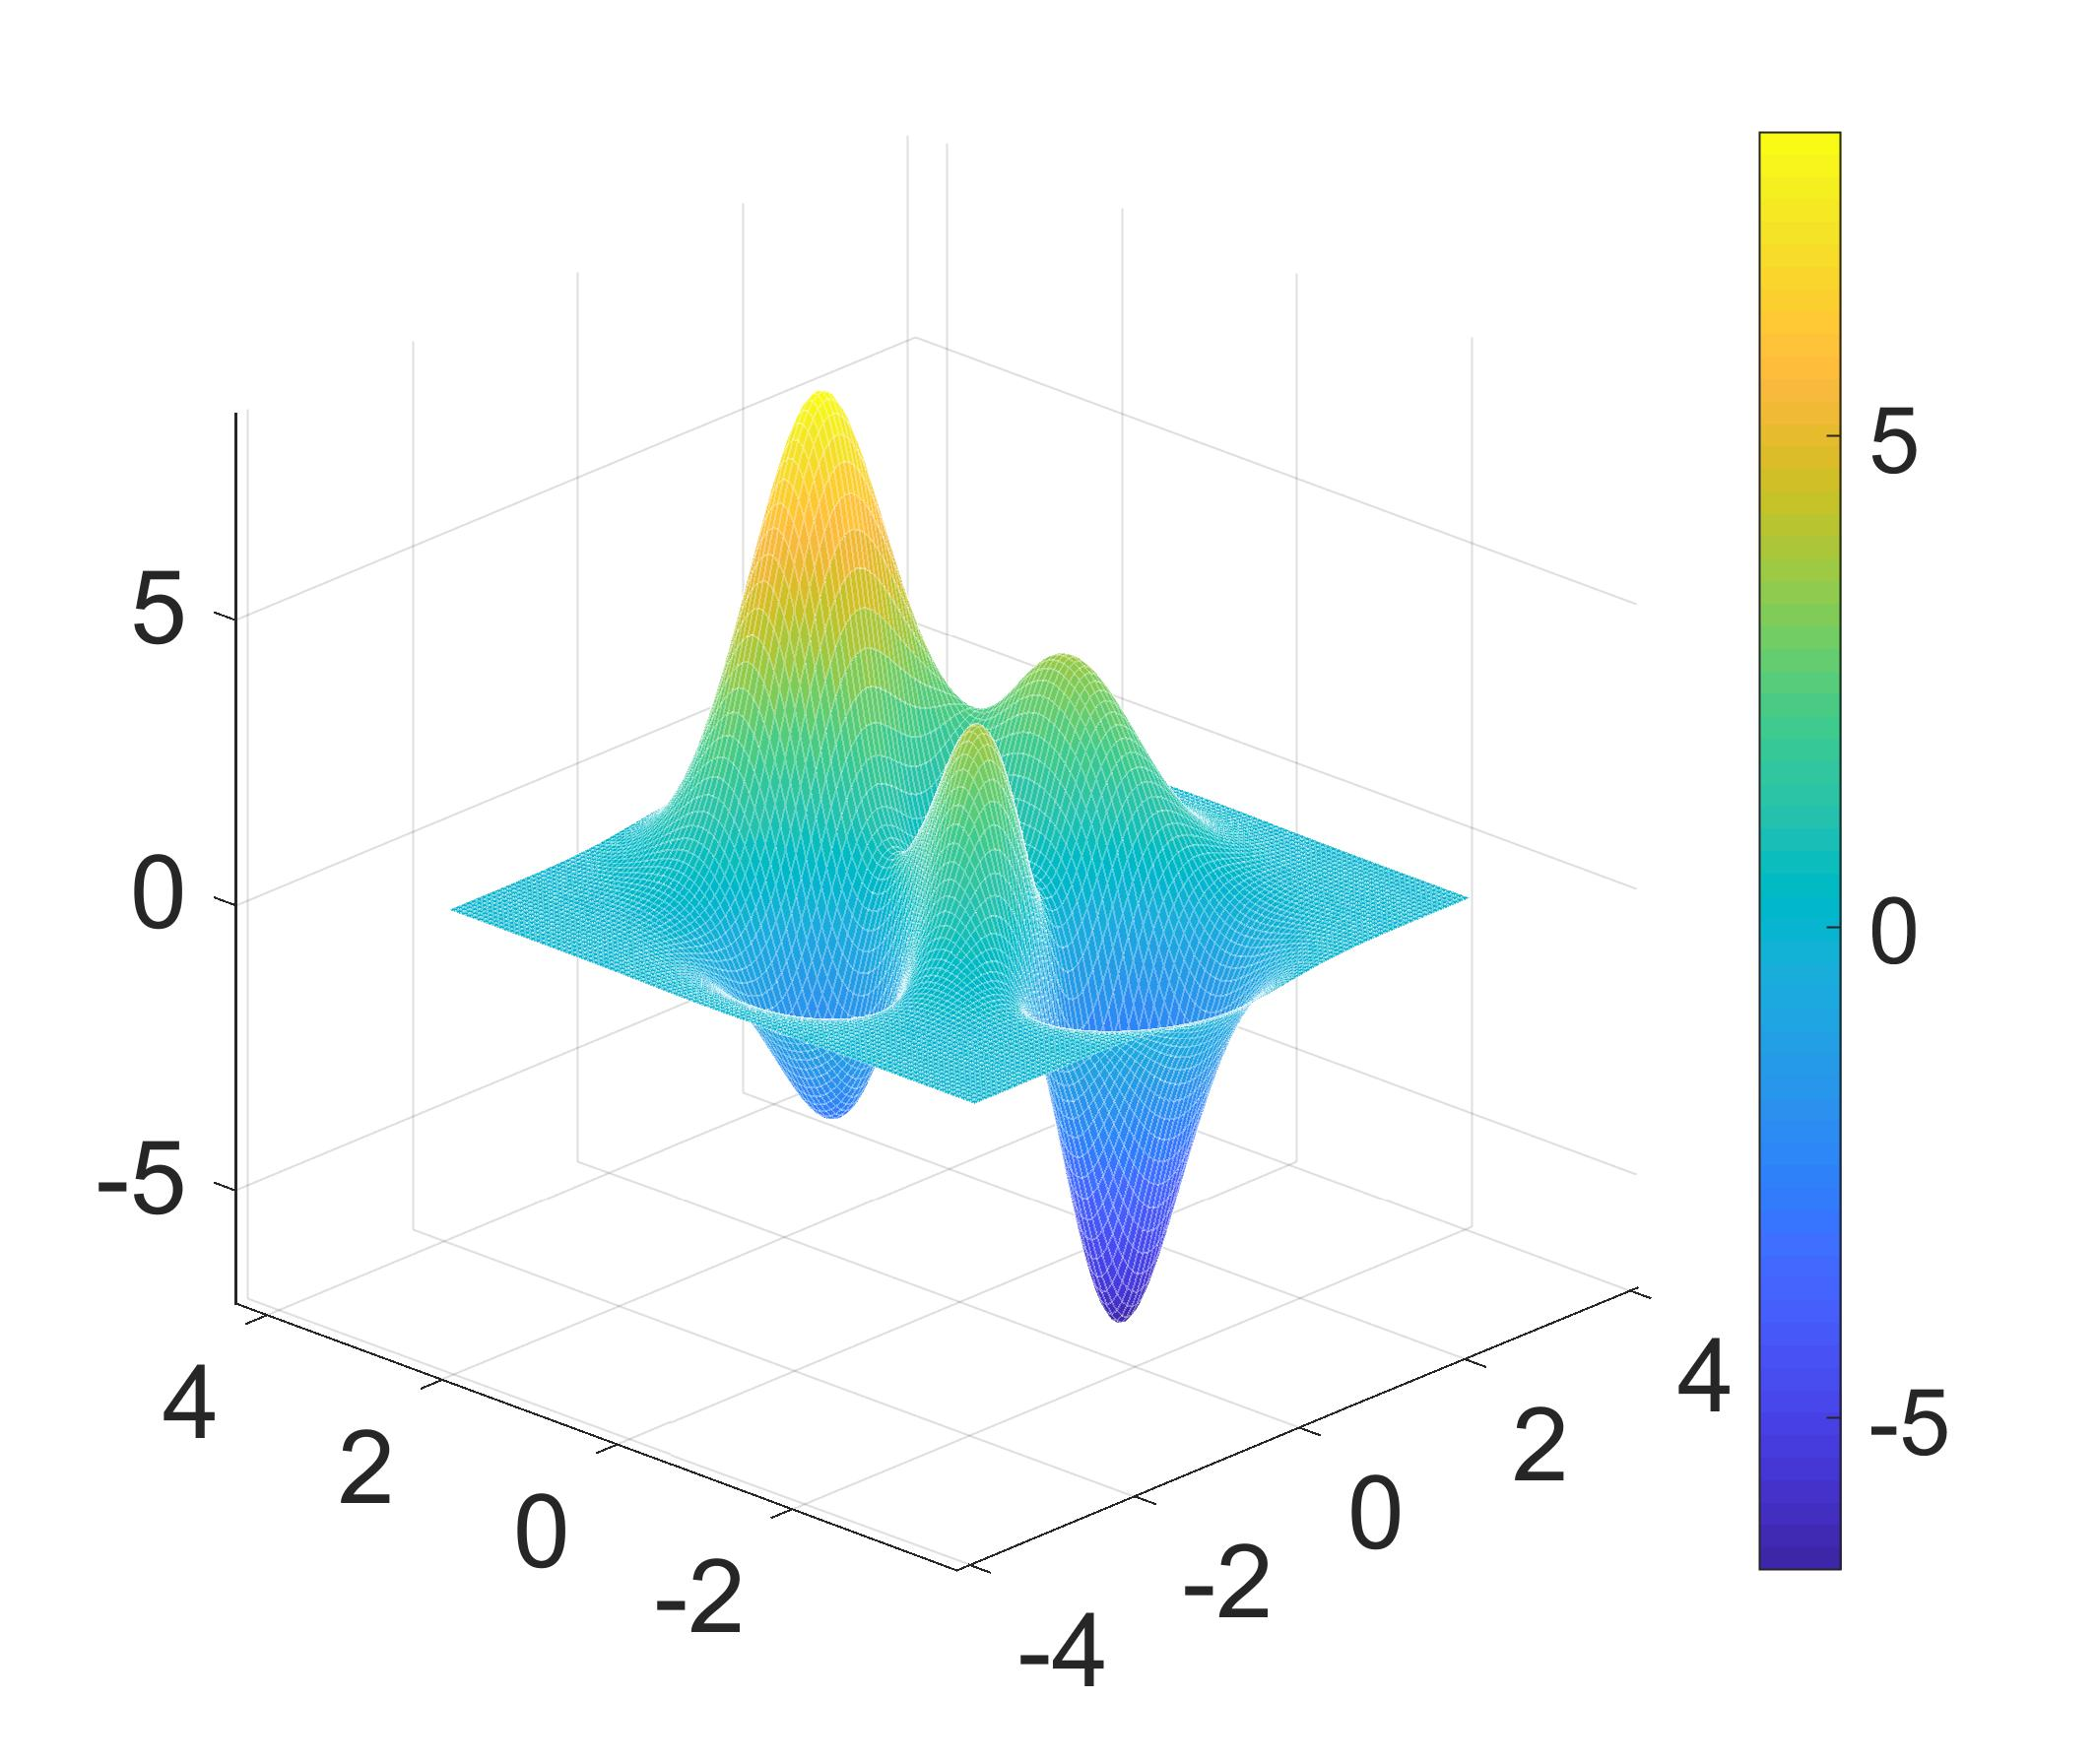
\includegraphics[width=\textwidth, height=\textwidth]{"Part 2 - Search-Based Optimization/Particle Swarm Optimization/Images/FIG1.1.jpg"}
    \caption{Peaks function.}
    \label{fig:f1}
  \end{subfigure}
  \hfill
  \begin{subfigure}[b]{0.5\textwidth}
    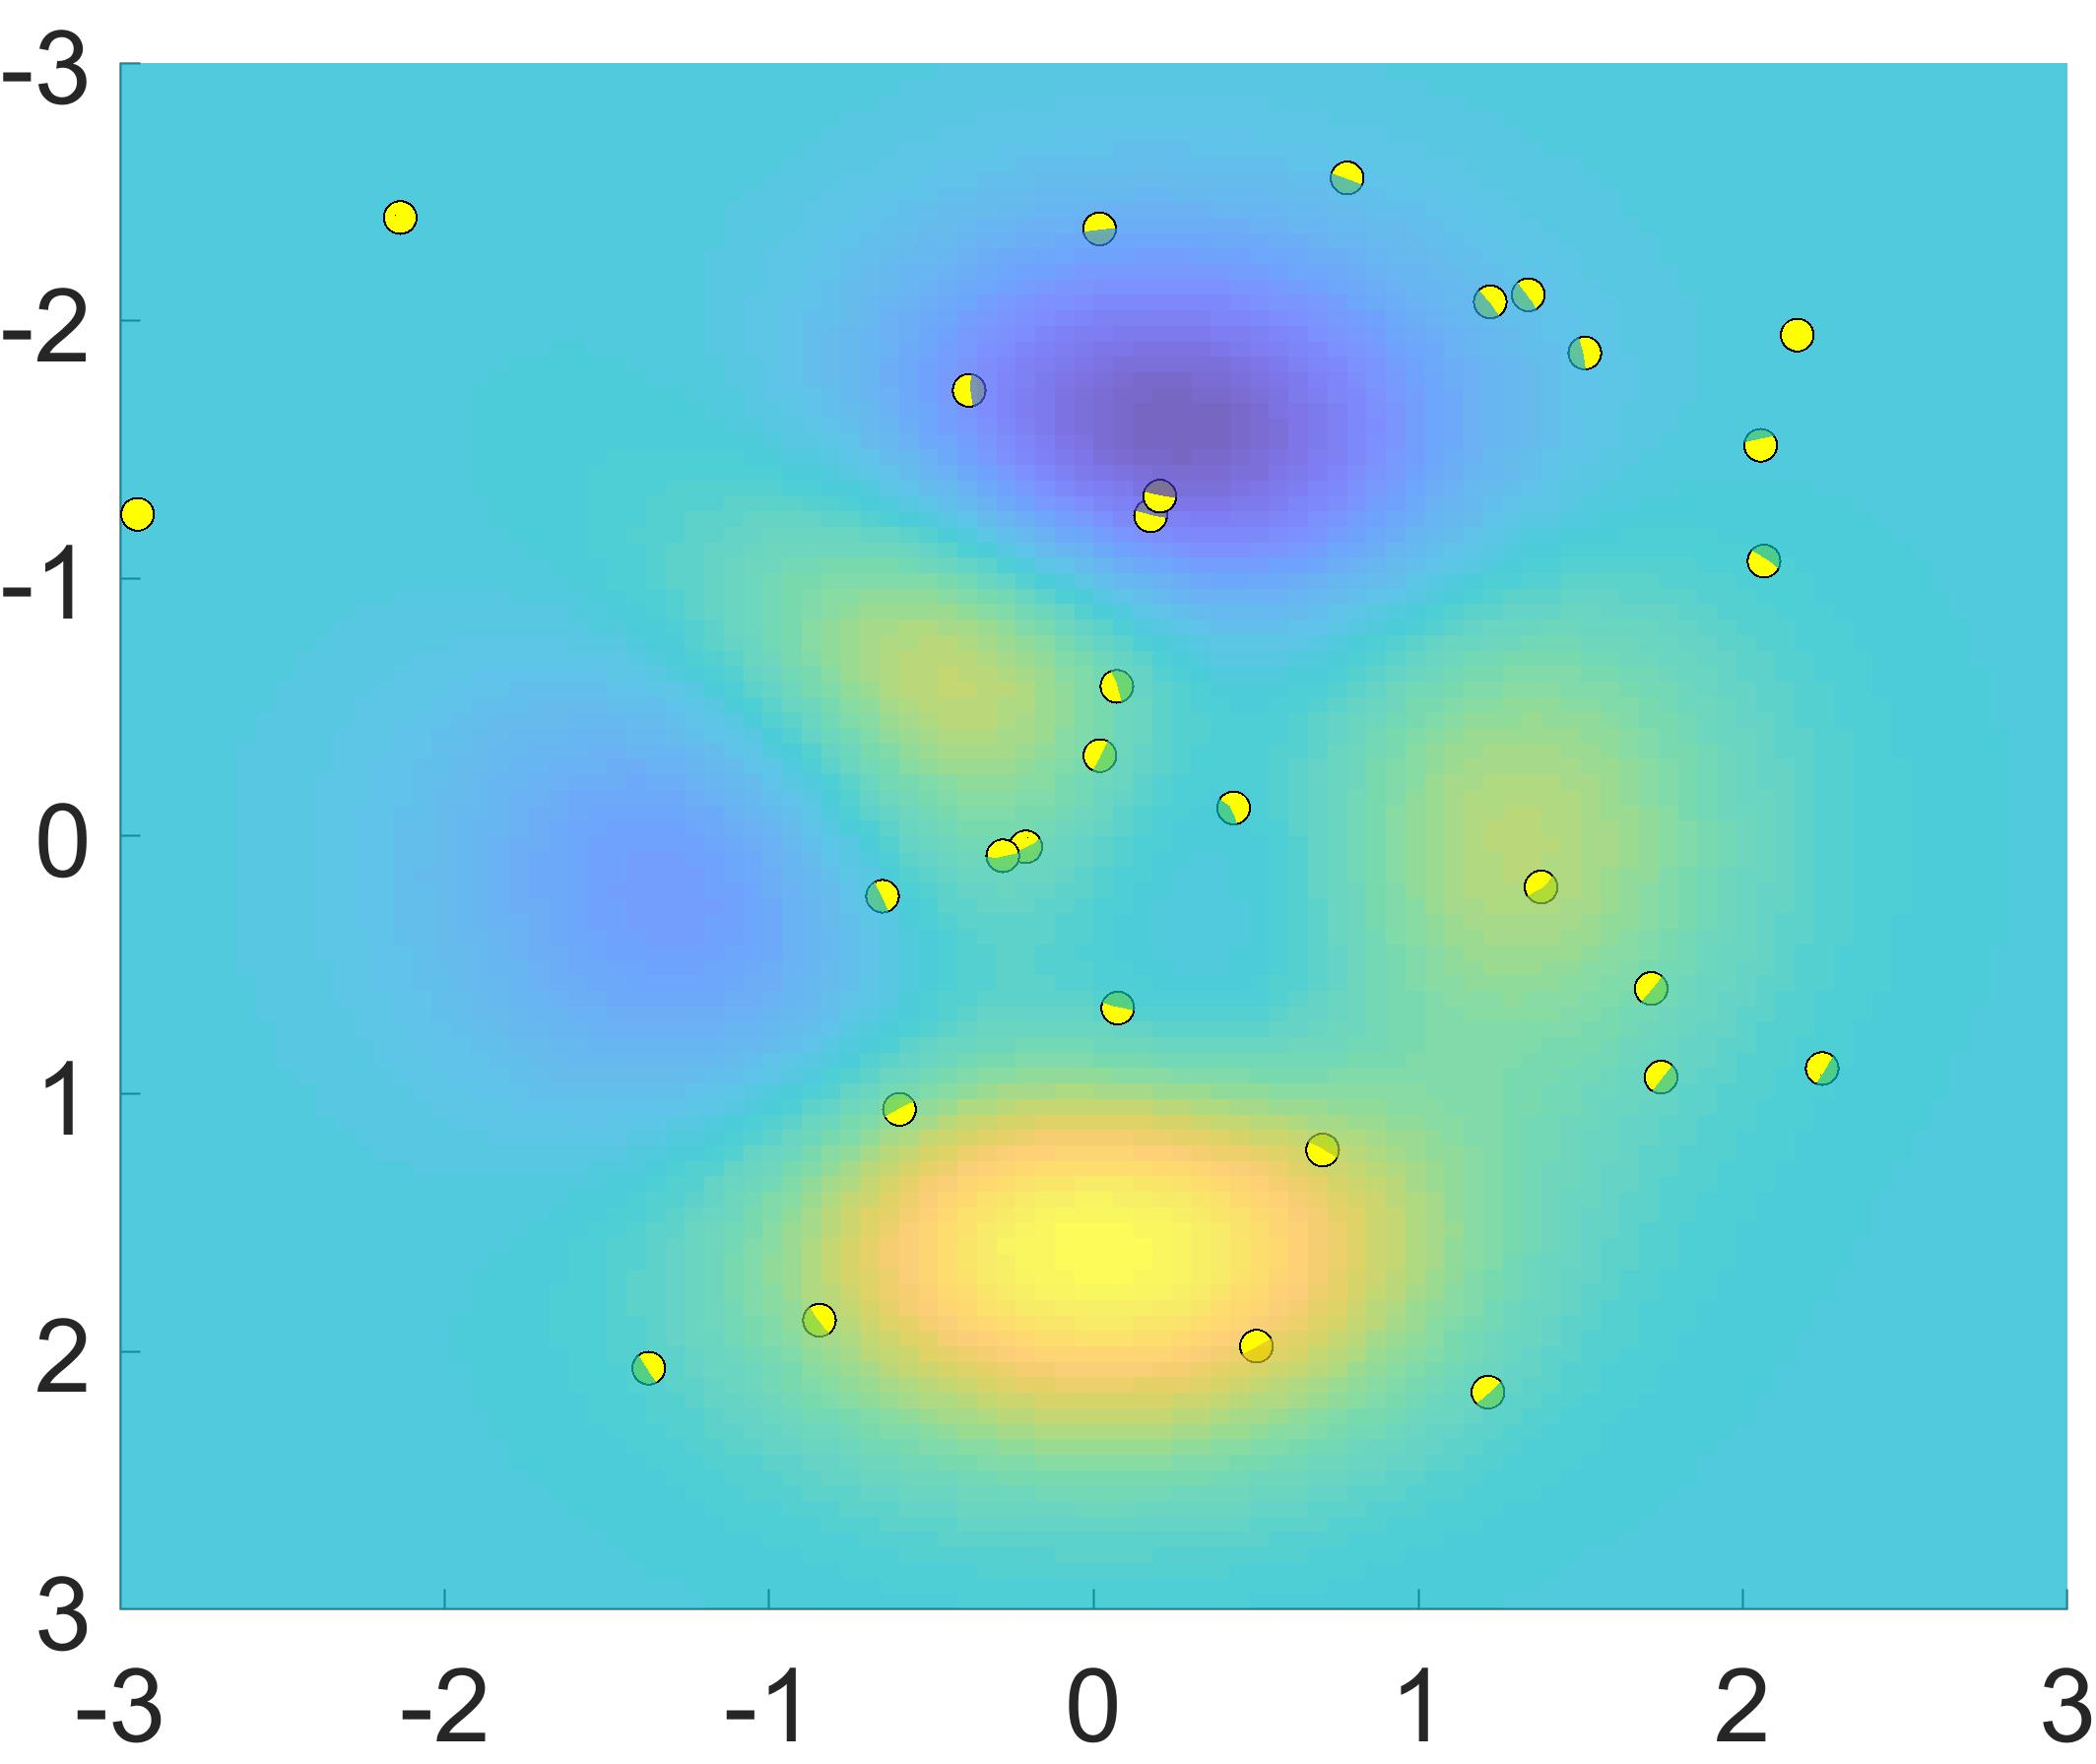
\includegraphics[width=\textwidth, height=\textwidth]{"Part 2 - Search-Based Optimization/Particle Swarm Optimization/Images/FIG2.1.jpg"}
    \caption{Distribution of the swarm at the initialization.}
    \label{fig:f2}
  \end{subfigure}
  \begin{subfigure}[b]{0.5\textwidth}
    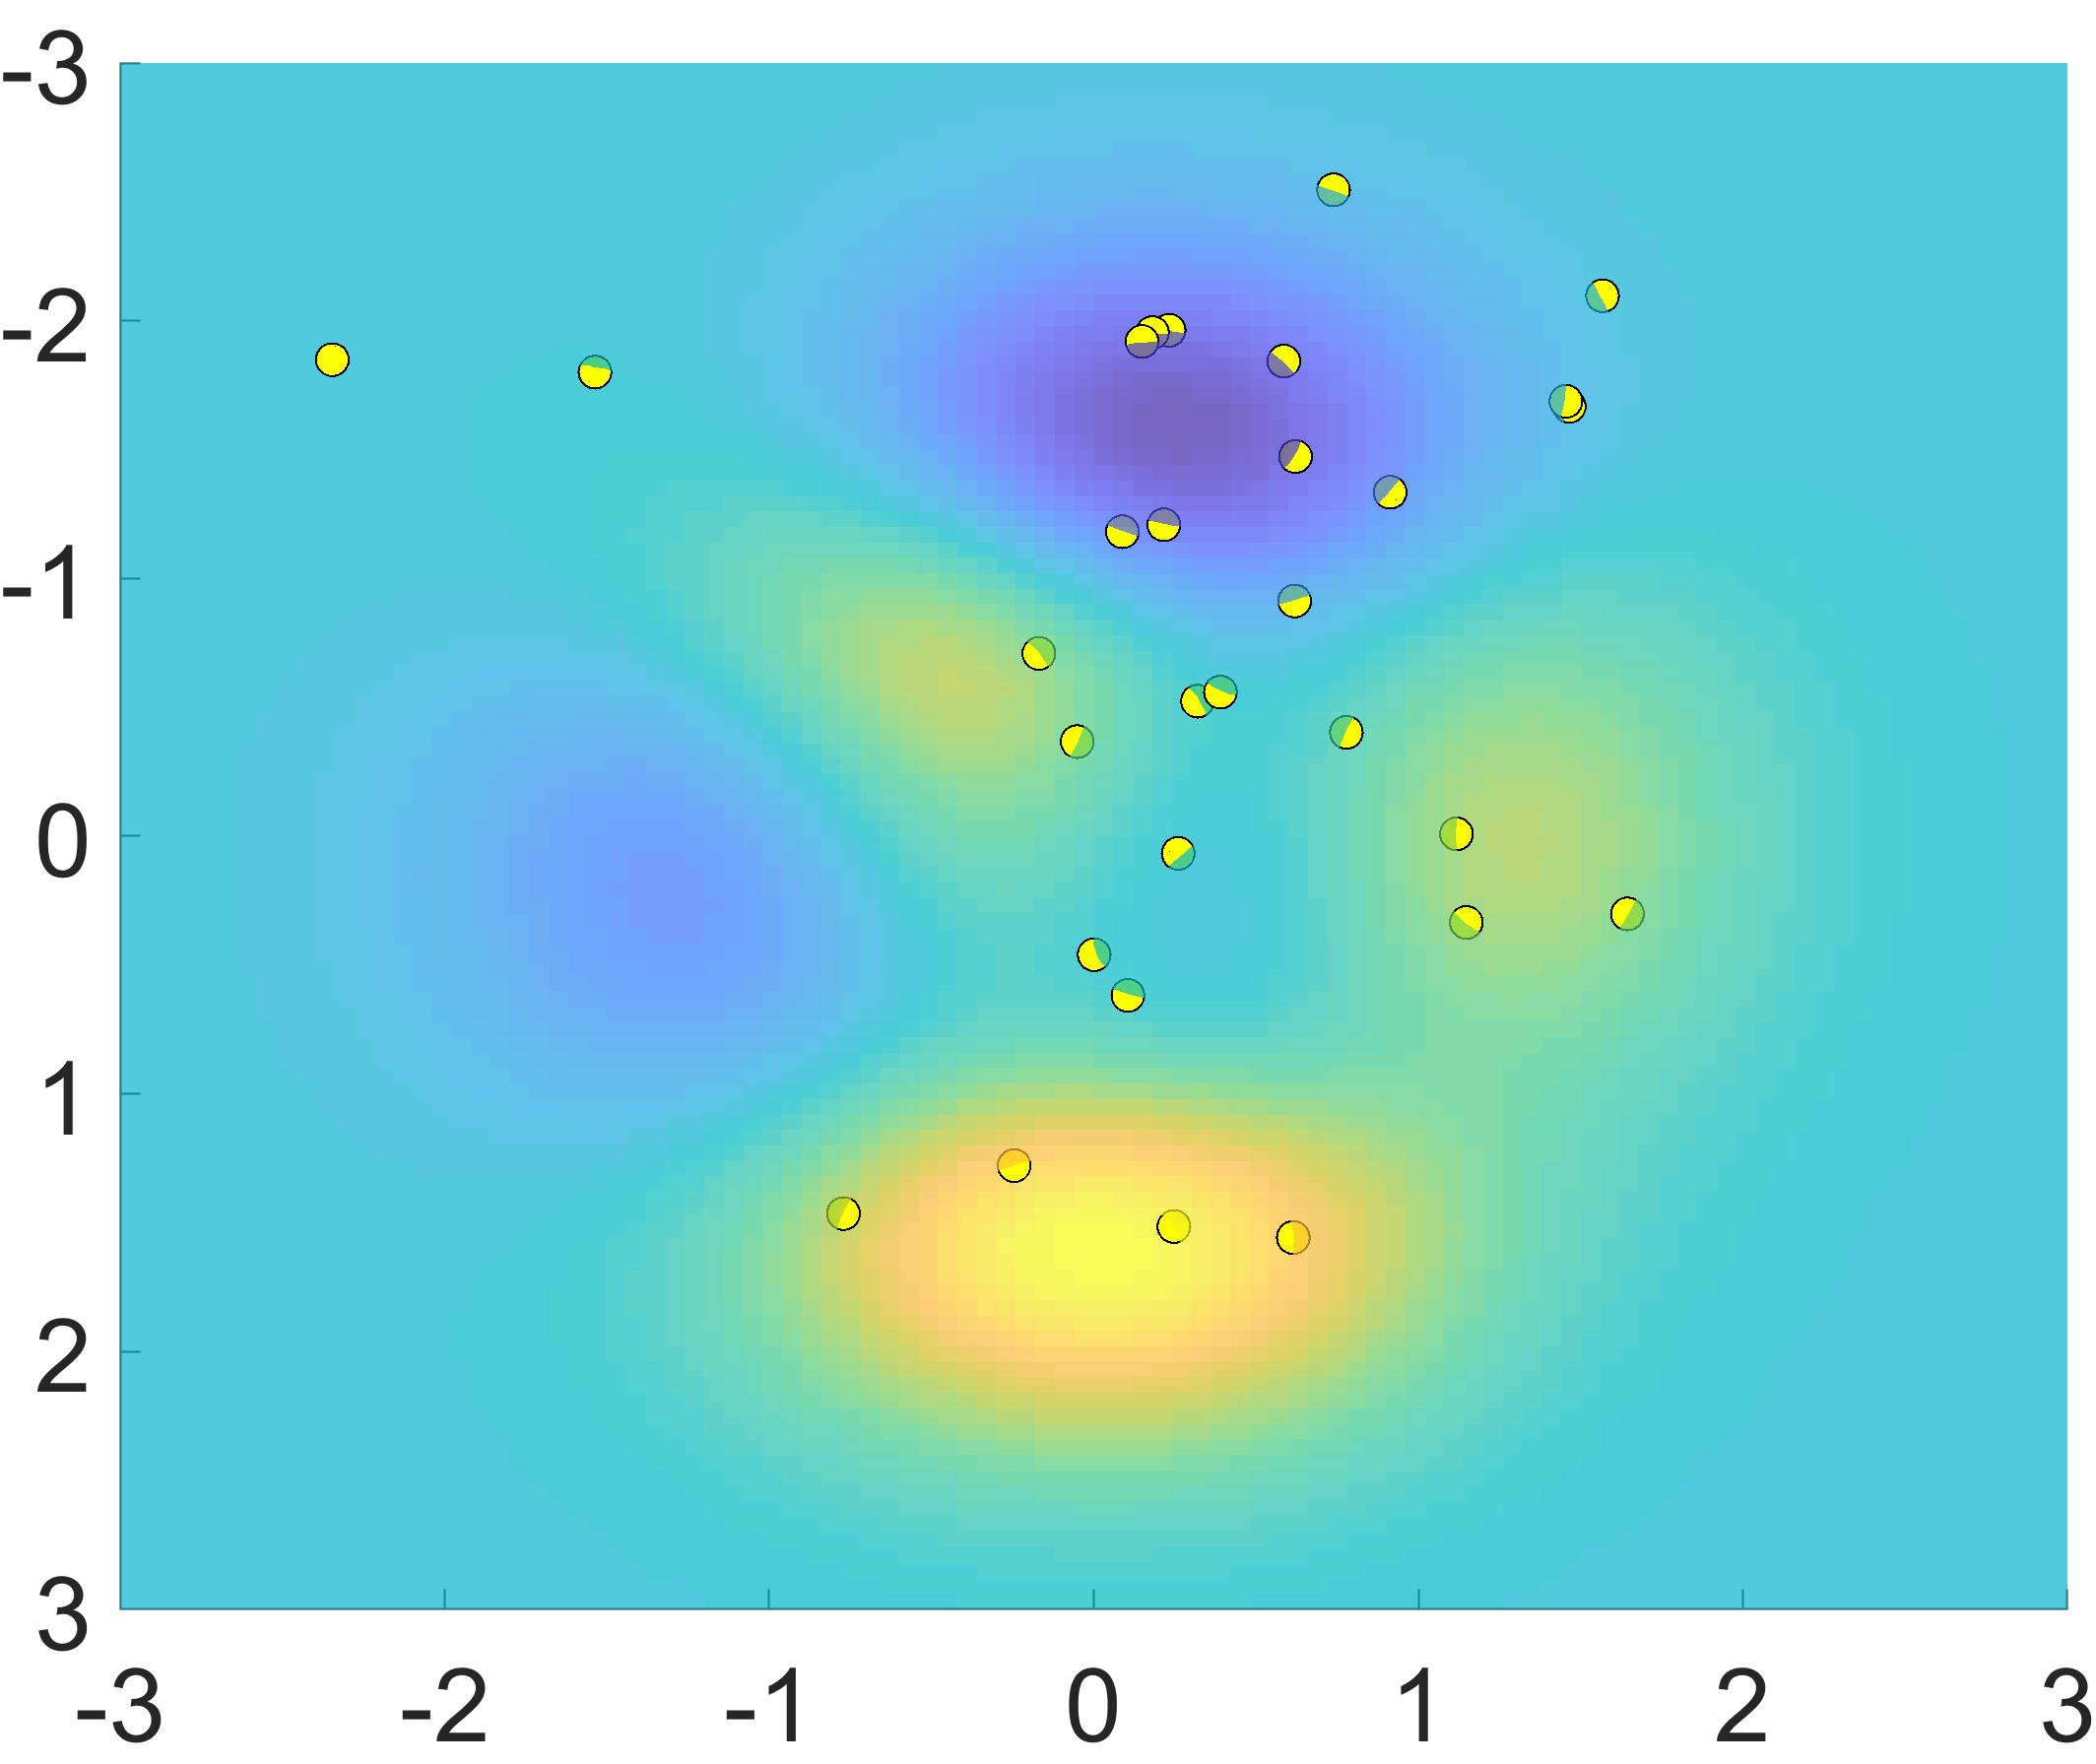
\includegraphics[width=\textwidth, height=\textwidth]{"Part 2 - Search-Based Optimization/Particle Swarm Optimization/Images/FIG3.1.jpg"}
    \caption{Distribution of the swarm at 50 iterations.}
    \label{fig:f3}
  \end{subfigure}
  \begin{subfigure}[b]{0.5\textwidth}
    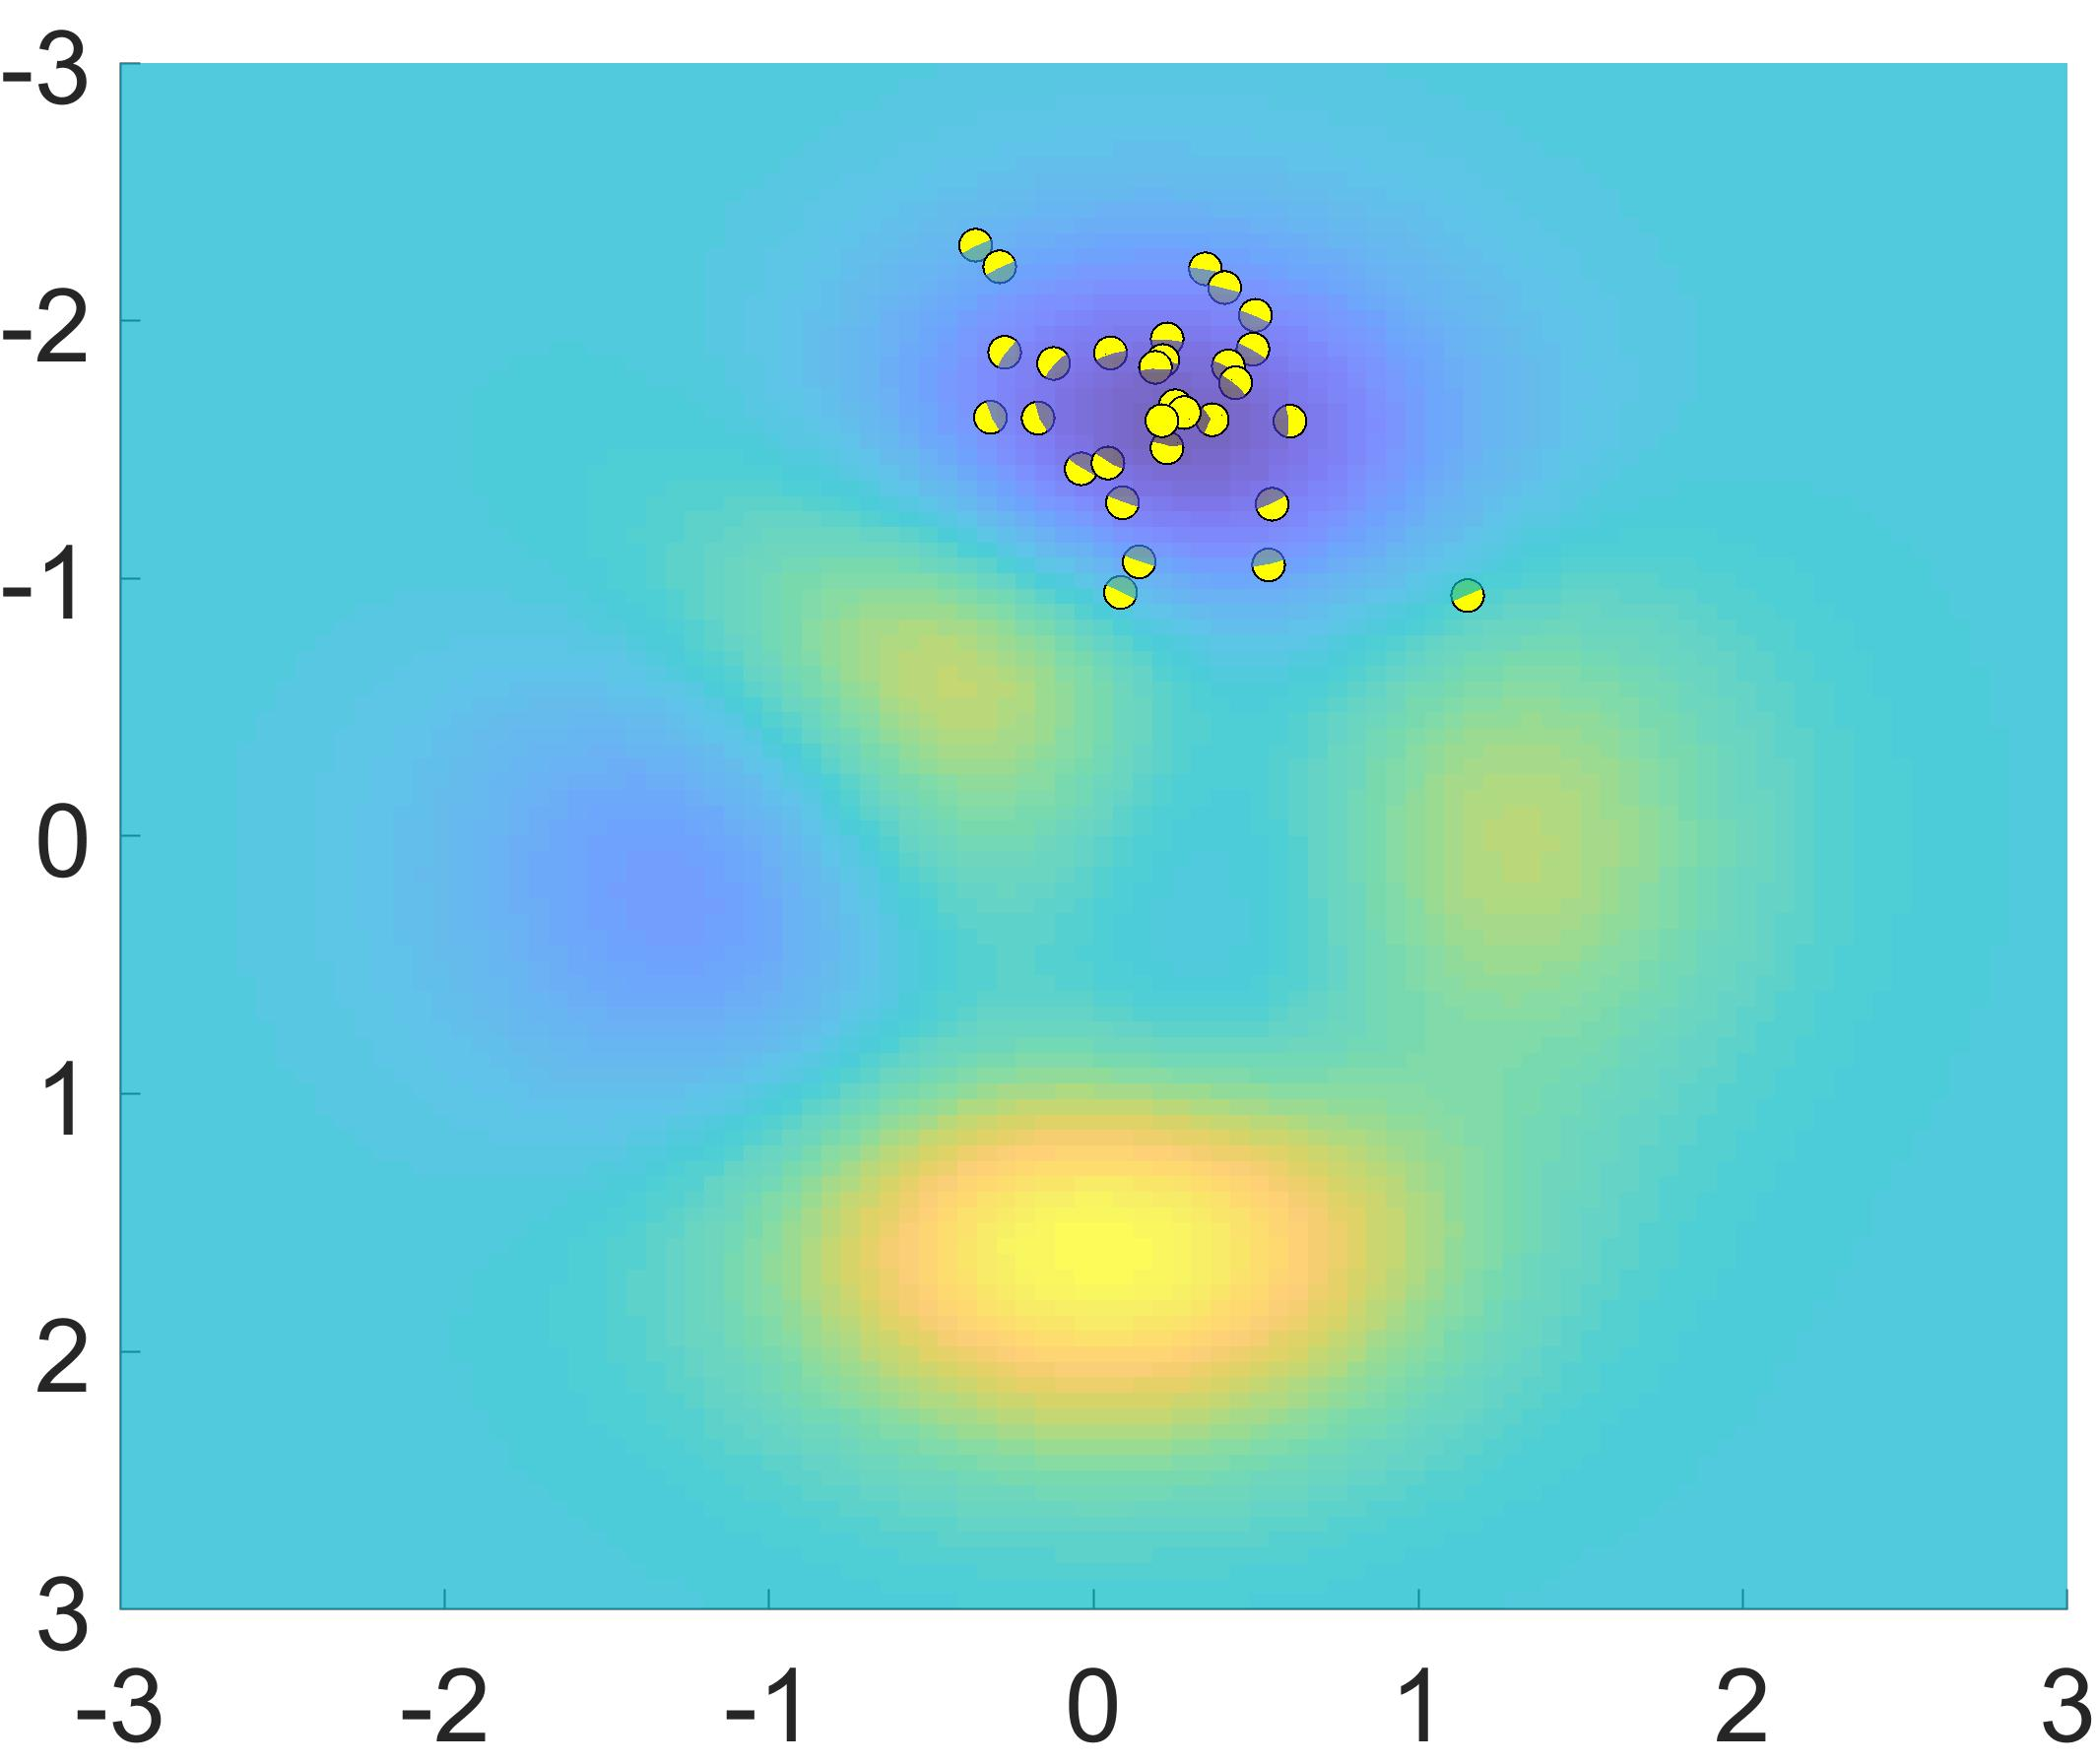
\includegraphics[width=\textwidth, height=\textwidth]{"Part 2 - Search-Based Optimization/Particle Swarm Optimization/Images/FIG4.1.jpg"}
    \caption{Distribution of the swarm at 300 iterations.}
    \label{fig:f4}
  \end{subfigure}
  \begin{subfigure}[b]{0.5\textwidth}
    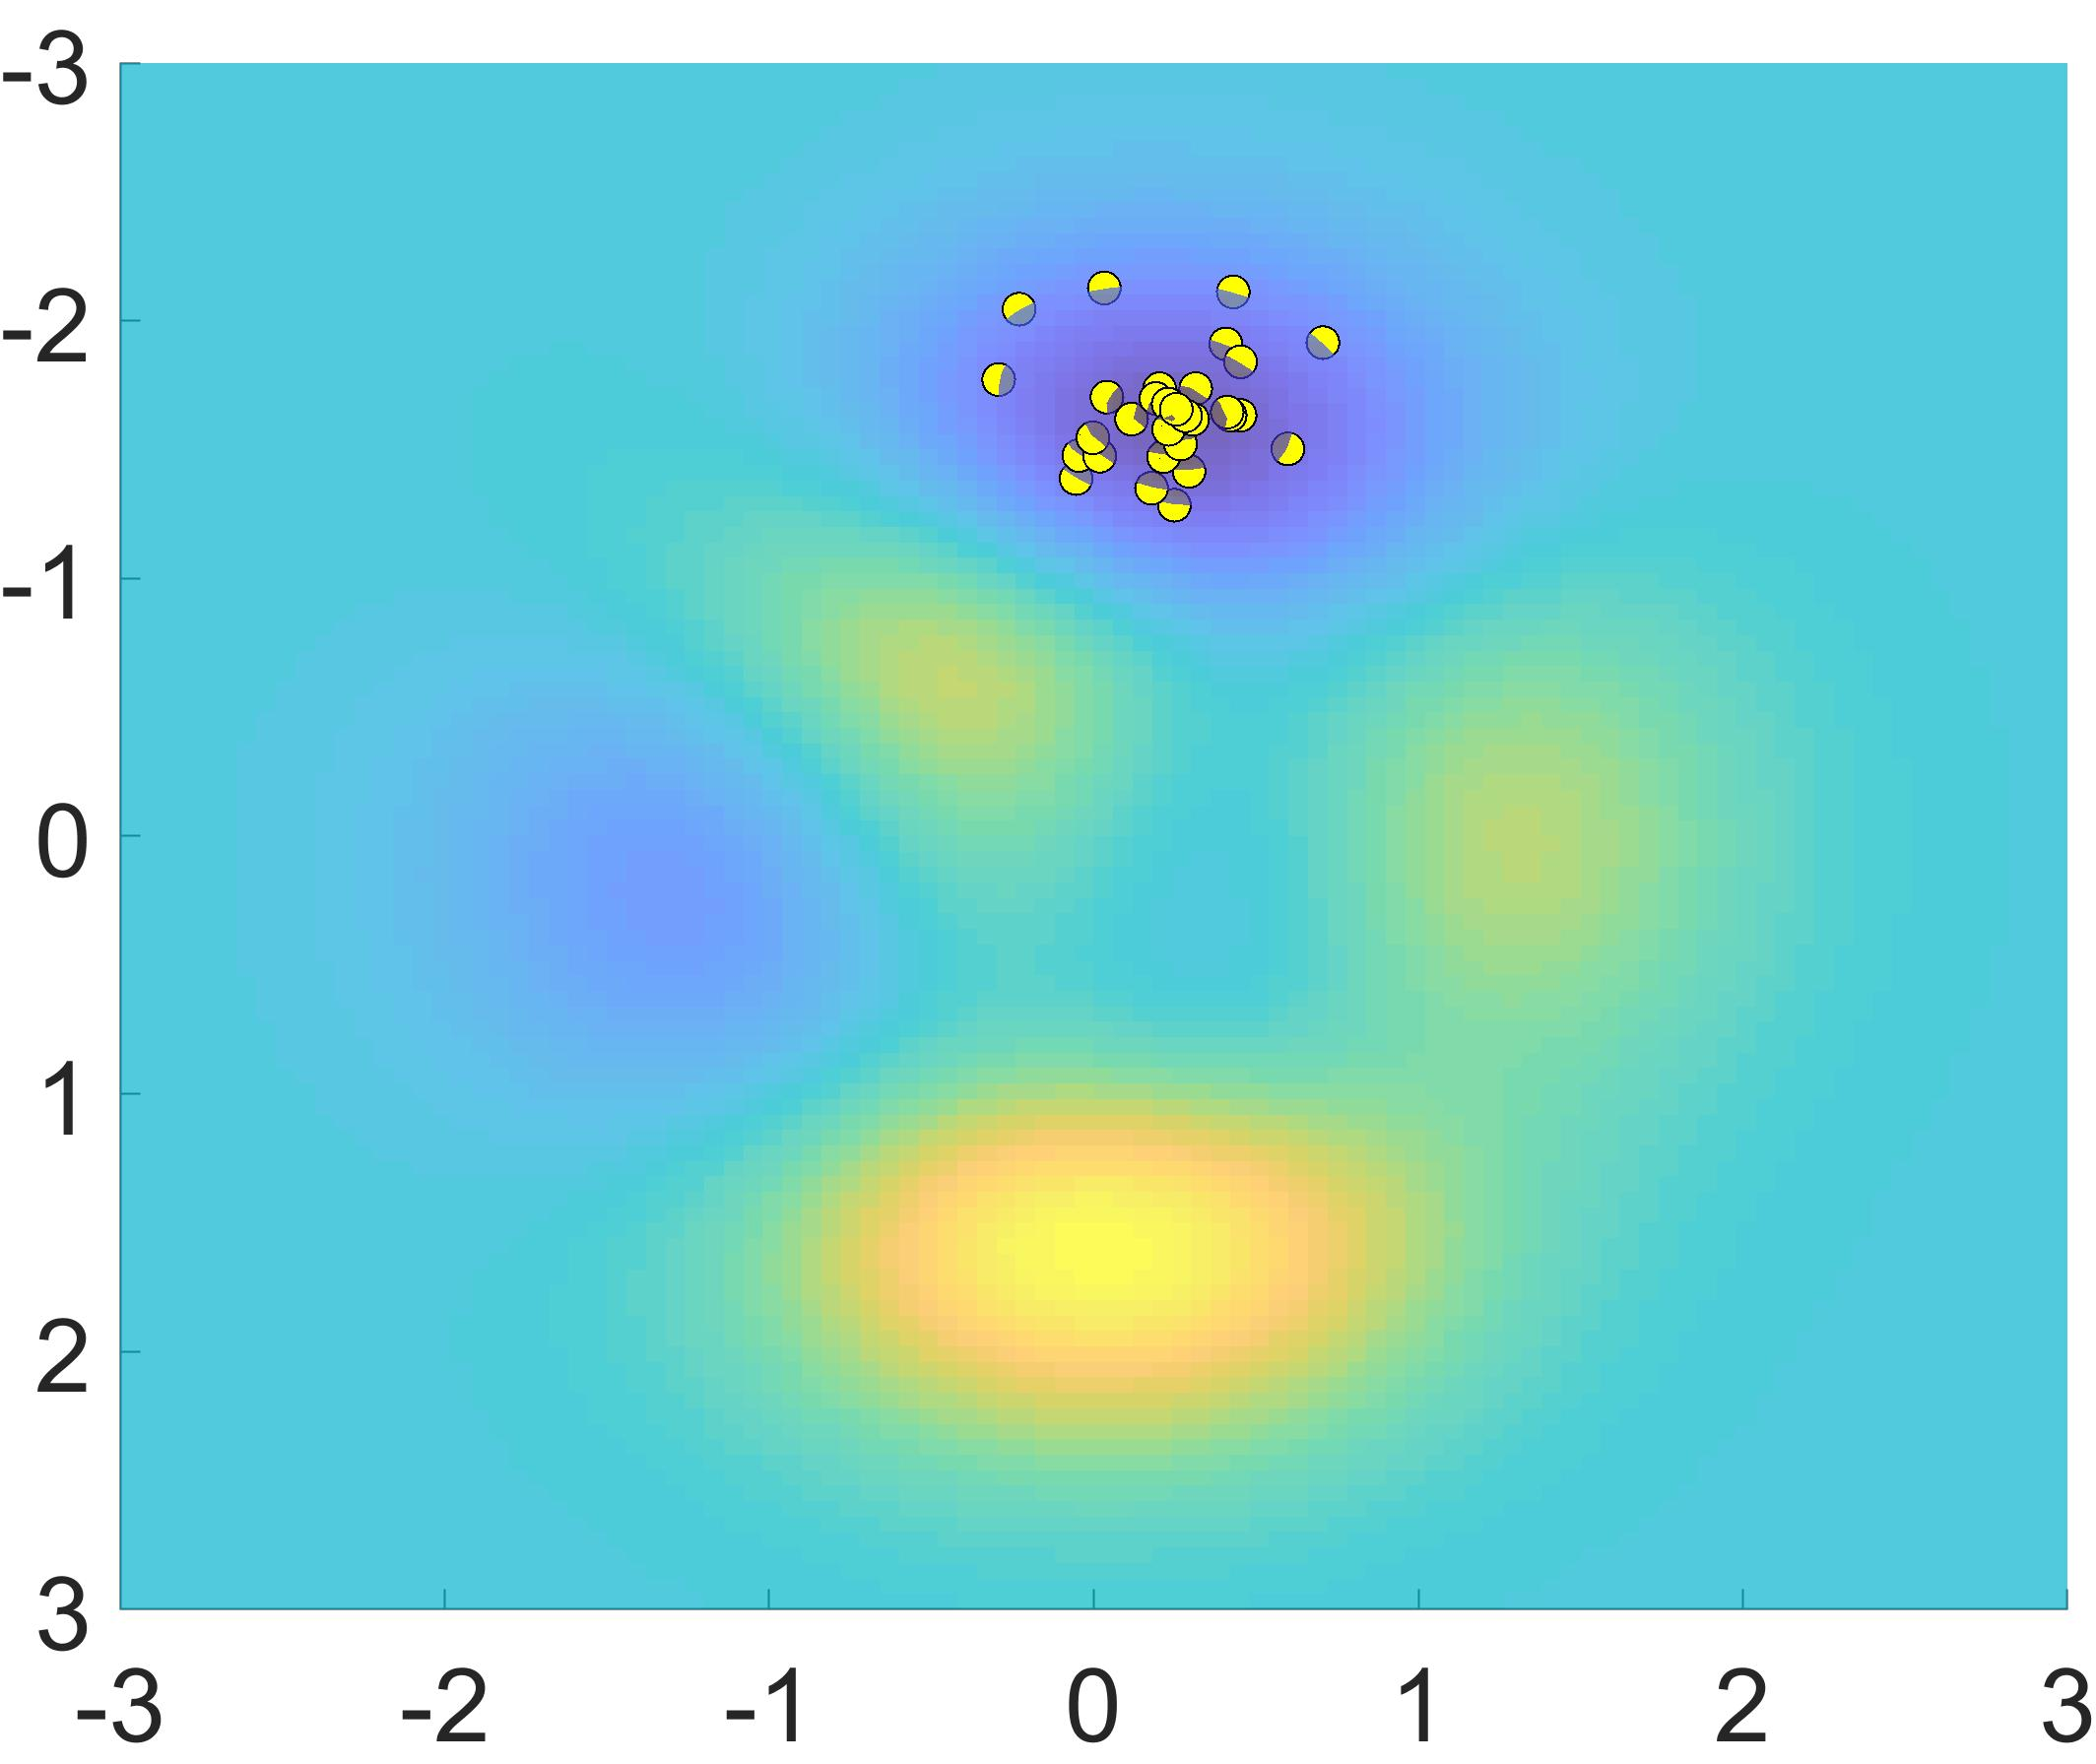
\includegraphics[width=\textwidth, height=\textwidth]{"Part 2 - Search-Based Optimization/Particle Swarm Optimization/Images/FIG5.1.jpg"}
    \caption{Distribution of the swarm at 600 iterations.}
    \label{fig:f5}
  \end{subfigure}
   \begin{subfigure}[b]{0.5\textwidth}
    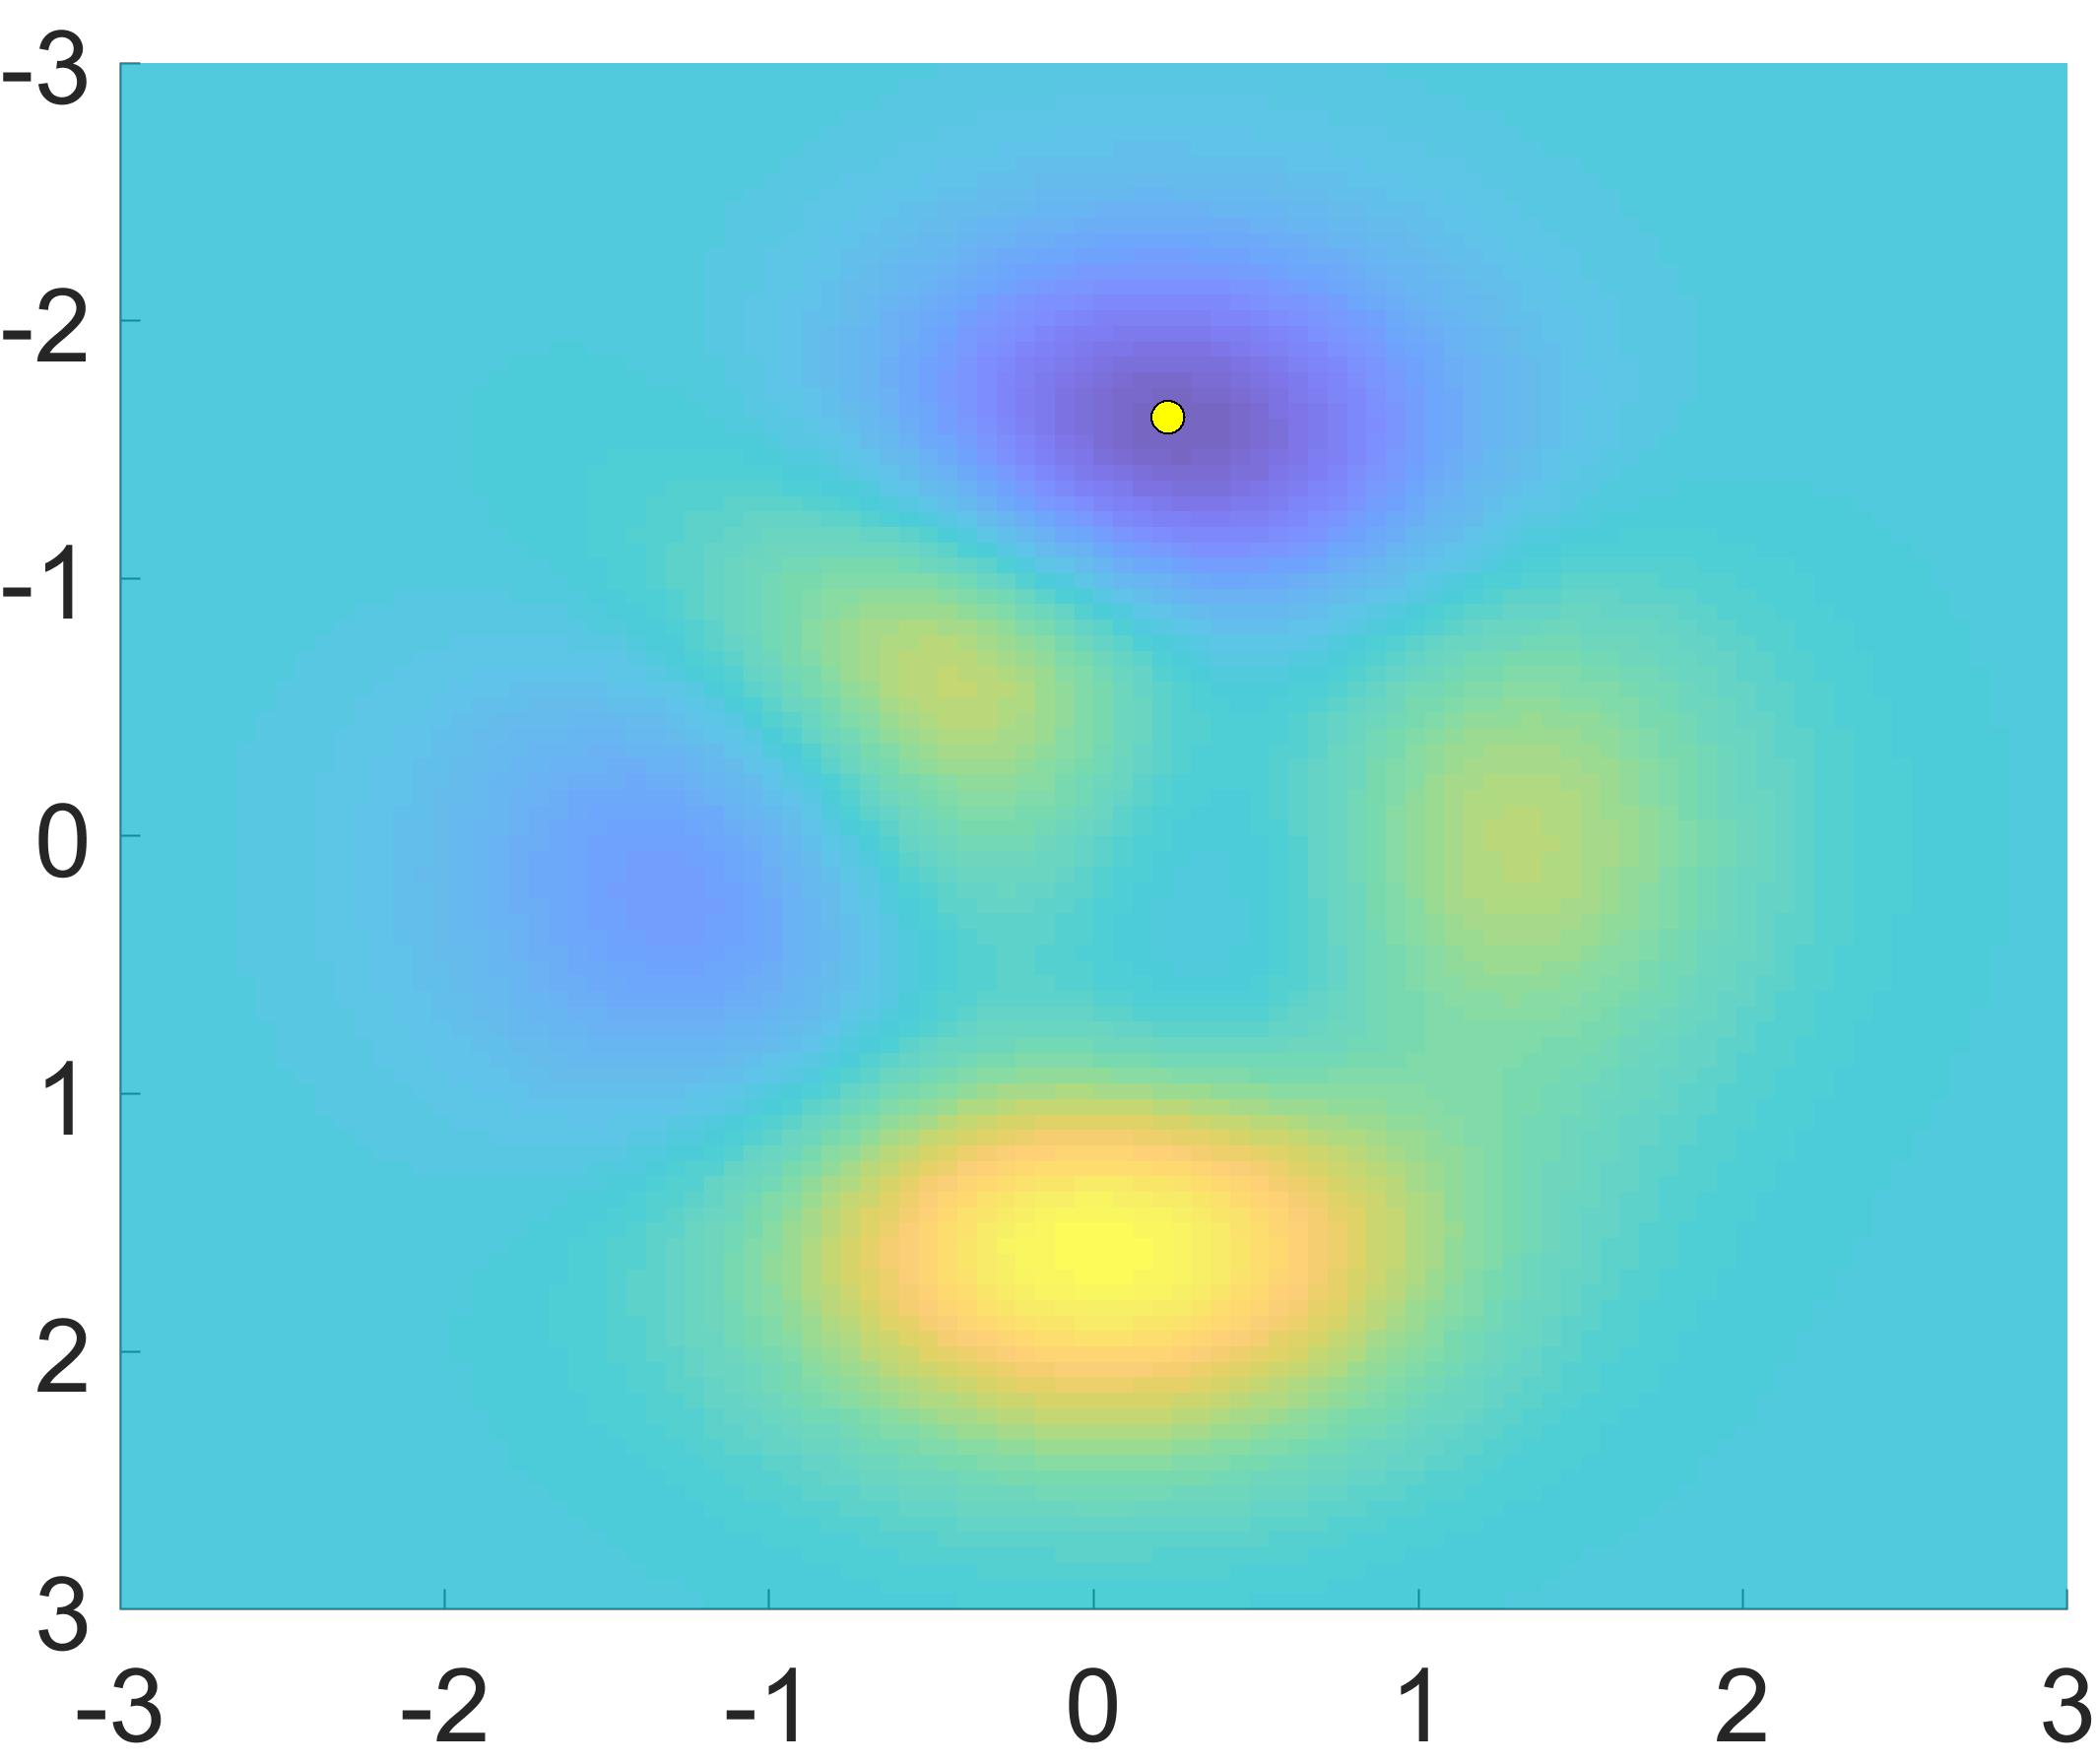
\includegraphics[width=\textwidth, height=\textwidth]{"Part 2 - Search-Based Optimization/Particle Swarm Optimization/Images/FIG8.1.jpg"}
    \caption{Final distribution of the swarm at 999 iterations.}
    \label{fig:f6}
  \end{subfigure}
  \caption{An example of the PSO along the iterative process.}
  \label{fig:fplots}
\end{figure}

%Optimization problems are problems where we want to find solutions that minimize or maximize one or more objective functions, potentially subject to certain constraints. Some examples are:

%\begin{itemize}
%\item Routing problems, e.g., to find a path from a city of origin to a city of destination that minimizes the distance travelled, while ensuring that non-existent direct paths between any two cities are not used. 
%\item Bin packing problems, e.g., to find an assignment of items to bins that minimizes the number of bins used, while ensuring that the maximum volume of the bins is not exceeded.
%\item Scheduling problems, e.g., to find an allocation of staff to tasks in a software project, so as to minimize the cost and duration of this project, while ensuring that staff are only allocated to tasks for which they have the necessary skills.
%\item Hyperparameter optimization, e.g., to find the hyperparameter values that minimize the loss (error) on the validation set for a given machine learning algorithm.
%\end{itemize}

%As we can see, in all examples above, we are interested in minimizing or maximizing a certain function (e.g., the distance travelled, the number of bins used, the cost and duration of the project and the error on the validation set). And, several these problems specify certain constraints (e.g., ensuring that non-existent direct paths are not used, ensuring that the maximum volume of the bins is not exceeded, and ensuring that staff have the necessary skills). Candidate solutions to optimization problems are referred to as \textit{feasible} if they satisfy the constraints of the problem, and \textit{infeasible} when they fail to satisfy one or more constraints.

%The examples above have been mentioned in rough terms, to give a general idea of what optimization problems are. In Section \ref{sec:formulation}, we will see what needs to be specified to formulate them more formally, so that they can be solved by optimization algorithms.


%\subsection{Optimization Algorithms}

%Optimization algorithms are algorithms that attempt to find solutions to optimization problems. They typically create one (or more) full initial candidate solutions to the problem, and then try to iteratively improve such candidate solution(s) in an attempt to find an optimal solution. This is different from search tree-based search algorithms, which attempt to systematically explore the search space to find actions that build a solution over time. 

%For example, consider a routing problem where we wish to find a path to go from a given city A to city F. Consider also that cities B, C, D, E, G, H are also cities in the map. A search tree-based algorithm would start with city A, and then it may add city B to this path, and then add city C, and so on, until a full path between city A and city F is found. Such path is being constructed over time by systematically exploring the space of possible paths in the problem.

%Different from that, an optimization algorithm to solve a routing problem might start with an initial solution which consists of a vector of cities [A, B, C, G]. The algorithm would consider this to be a full \textit{candidate} solution to the problem, despite being infeasible, as it does not reach the destination city F. The algorithm would then modify this candidate solution over time, possibly by replacing, adding or removing cities, in an attempt to find better candidates solutions to the problem. 

%Optimization algorithms typically do not maintain a data structure to store all the explored portion of the space of possible solutions to the problem, being usually more space-efficient than search tree-based algorithms. Several optimization algorithms from the artificial intelligence literature are also more time efficient than the search tree-based algorithms, depending on the problem that is being solved. In addition, they usually don't require problem-specific heuristics that are difficult to design, which is an advantage over search algorithms such as A*. Optimization algorithms from the artificial intelligence literature are frequently \textit{not guaranteed} to find optimal or feasible solutions, but will frequently be able to find good (or near optimal) solutions in a reasonable amount of time.


%\subsection{Formulating Optimization Problems}
%\label{sec:formulation}

%Without loss of generality, an optimization problem is a problem with the following general form:
%\[
%\begin{tabular}{ll}
%minimize        & $f_k(\mathbf{x})$, \ \ \ \ \ \ \ \ \ \ \ $k=\{1,2,\cdots,p\}$ \\ 
%subject to      & $g_i(\mathbf{x}) \leq 0$, \ \ \ \ \ $i=\{1,2,\cdots,m\}$ \\
%                & $h_j(\mathbf{x}) = 0$, \ \ \ \ \ $j=\{1,2,\cdots,n\}$ \\
%\end{tabular}
%\]

%Here, we wish to find a solution $\mathbf{x} \in \mathcal{X}$ that minimizes the functions $f_k(\mathbf{x})$ while satisfying the constraints $g_i(\mathbf{x}) \leq 0$ and $h_i(\mathbf{x}) = 0$, where $p$ is the number of objective functions to be optimised, $m$ is the number of constraints of the type $g_i$ and $n$ is the number of constraints of the type $h_j$ and $\mathcal{X}$ is the domain of $\mathbf{x}$. 

%Such kind of problem contains three main components:
%\begin{itemize}
%\item \textit{Design variable} $\mathbf{x}$. This is the variable that represents candidate solutions to the optimization problem. The domain $\mathcal{X}$ of $\mathbf{x}$ depends on the optimization problem, and could consist of numeric, categorical or ordinal variables, a mix of these, or any other kind of variable that may be relevant to the problem. In addition, $\mathbf{x}$ is not necessarily a vector. It could be any other kind of data structure that may be relevant to the problem in hands. For example, if one is trying to allocate staff members to tasks in a problem, it would be reasonable to consider that $\mathbf{x}$ is a matrix where the rows represent staff members and the columns represent tasks, where each position $x_{i,j}$ contains the value 1 if staff member $i$ is allocated to task $j$ and 0 otherwise. The design variable and its domain define the \textit{search space} of the optimization problem. This is the space of all possible candidate solutions to the problem.

%\item \textit{Objective function(s)} $f_k(\mathbf{x})$, where $k=\{1,2,\cdots,p\}$. These are the functions that we wish to optimise (maximize or minimize). We refer to a problem where $p=1$ as a single-objective optimization problem, and to a problem where $p>1$ as a multi-objective optimization problem. When dealing with a single-objective optimization problem, the $k$ value is frequently omitted from the name of the objective function, i.e., we typically write $f(\mathbf{x})$ instead of $f_1(\mathbf{x})$. You may also hear the term many-objective optimization problems when there are $p>3$ objectives. You will note that the general form above lists a minimisation problem. We can also replace ``minimize'' by ``maximize'' in the general form above if we are dealing with a maximisation problem. It is also possible to use a mix of objectives to be minimized and maximized. However, it is possible to convert maximisation problems into minimisation problems, reason why the general form above lists only minimisation without loss of generality. 

%\item \textit{Constraint(s)}  $g_i(\mathbf{x}) \leq 0$ and $h_j(\mathbf{x}) = 0$, where $i=\{1,2,\cdots,m\}$ and $j=\{1,2,\cdots,n\}$. These are the constraints that a candidate solution $\mathbf{x}$ must satisfy in order to be a feasible solution to the problem. The $g_i$ type of constraints are called inequality constraints, whereas the $h_j$ type of constraints are called the equality constraints. When $m=0$ and $n=0$, the problem is called an unconstrained optimization problem. When $m>0$ or $n>0$, the problem is called a constrained optimization problem. Problems may also involve constraints with inequalities of the type $\geq$ instead of $\leq$. However, it is possible to convert inequalities of the type $\geq$ to inequalities of the type $\leq$, reason why the general form above lists only $\leq$ without loss of generality \footnote{Strict inequalities ($>$ or $<$) are typically not used in optimization problems, as they can lead to ill-posed problems. For instance, consider a problem where we wish to minimize $f(x) = x^2$, subject to $x>0$, where $x$ is a real value. Had the constraint been $x \geq 0$, the optimal solution would have been $x=0$. However, as the constraint is $x>0$, there is no minimizing value. You can always get $x$ values that are closer and closer and close to zero, without ever reaching a minimum. Alternatively, if $x$ was an integer value, this problem would not occur. However, in this case it would be possible to convert the strict inequality $x>0$ into the inequality $x\geq 1$, meaning that the general form of the optimization problem does not need to have strict inequality constraints.}.
%\end{itemize}

%In order to formulate an optimization problem, all the components above must be specified. The more mathematical the problem formulation is, the less ambiguous it is likely to be. However, more mathematical formulations may become more abstract, meaning that it may become more difficult to understand its underlying meaning in the context of the problem of interest. Therefore, it is advisable to provide a problem formulation that is the most formal (mathematical) possible, while including an explanation of it using natural language. %Some examples of problem formulations are provided in the lecture slides.

%\section{Dealing with Constraints}
%
%Optimization algorithms from the artificial intelligence literature frequently don't include themselves strategies to deal with constraints. Instead, we need to design such strategies. There are many different ways to deal with constraints in optimization algorithms. Two examples of strategies are the following:
%
%\begin{itemize}
%\item Representation, initialisation and neighbourhood operators: this kind of strategy requires to design a representation, initialisation procedure and neighbourhood operators that do not allow any infeasible solution to ever be generated by the optimization algorithm. Its advantage is that it makes the optimization algorithms complete, i.e., guaranteed to find feasible solutions. Its disadvantage is that it is problem-dependent and thus not easy to design. Moreover, it may restrict the search space too much, which can sometimes hinder the search for optimal solutions. In the worse case scenario, such restrictions may eliminate the optimal solution from the reachable areas of the search space, meaning that the optimal solution cannot be found. 
%
%Some optimization algorithms are not based on neighbourhood operators, but other kinds of operators. In such cases, these other kinds of operators must also ensure that infeasible solutions are never generated.
%
%\item Objective function: it is possible to modify the objective function in order to penalise the objective values of infeasible solutions. Considering the general form of optimization problems shown in Section \ref{sec:formulation} with $k=1$, the objective function could be modified as shown below in order to deal with the constraints.
%
%\[
%\begin{tabular}{ll}
%minimize        & $f(\mathbf{x}) + Q(\mathbf{x})$\\
%subject to      & $g_i(\mathbf{x}) \leq 0$, \ \ \ \ \ $i=\{1,2,\cdots,m\}$ \\
%                & $h_j(\mathbf{x}) = 0$, \ \ \ \ \ $j=\{1,2,\cdots,n\}$ \\
%\end{tabular}
%\]
%
%\noindent where:
%
%\[ Q(\mathbf{x}) =
%  \begin{cases}
%    0       & \text{if } \mathbf{x} \text{ is feasible.}\\
%    P [g_a(\mathbf{x})^2 + g_b(\mathbf{x})^2 + \cdots + h_{a'}(\mathbf{x})^2 + h_{b'}(\mathbf{x})^2 + \cdots] & \text{otherwise}
%  \end{cases}
%\]
%
%\noindent where $P$ is a very large positive constant, and the indexes $a$, $b$, ..., $a'$, $b'$, ..., represent the indexes of the constraints that are violated. For example, consider a candidate solution $\mathbf{x}$ that violates only the constraints $g_2(\mathbf{x})$, $g_5(\mathbf{x})$ and $h_3(\mathbf{x})$. In this case, $Q(\mathbf{x}) = P [g_2(\mathbf{x})^2 + g_5(\mathbf{x})^2 + h_3(\mathbf{x})^2]$. The constant $P$ should ideally be large enough to make the objective value of infeasible solutions worse (larger) than the objective value of any feasible solution. The power of two used in the functions $g$ and $h$ ensures that the values of these functions will always be positive, such that the penalty will always increase (worsen) the objective value. % \footnote{The use of square can also help the optimization process depending on the optimization algorithm being adopted. This is because it causes the values of the objective function of infeasible solutions that violate a given constraint by different amounts to differ more from each other. For example, consider an infeasible solution $\mathbf{x}$ for which $g_a(\mathbf{x}) = 1$ and another infeasible solution $\mathbf{x}$ for which $g_a(\mathbf{x}) = 2$. The penalty applied to these }.
%
%The advantage of this strategy to deal with constraints is that it is very general. The same strategy could potentially be adopted for any optimization problem. However, as it enables infeasible solutions to be generated, the optimization algorithm would have to spend time searching for feasible solutions. For some problems where that are too many infeasible solutions, the algorithm may struggle to find feasible solutions based solely on the objective function, in which case the strategy based on representation, initialisation and neighbourhood operators may be more adequate. 
%
%An example of use of these two types of strategies to deal with constraints is provided in the lecture slides.
%
%
%\end{itemize}

\section{The PSO variants}
\label{sec:variants}

This algorithm has been so successful since its emergence that it has been the base for designing new methods. Same that preserves the essence and structure of the PSO but adds improvements in operators, parameters, initialization, or combines concepts that make the algorithm more specialized for specific problems. The most important variants are listed below, divided into two fields, single-objective and multi-objective optimization:\\ 

\subsection{Top PSO variants for single-objective problems}
\label{tab:pso_variants}
There are many publications related to PSO variants for single-objective optimization. Most of them were compiled and sorted by year of publication, adding the citations obtained from publication date up to the current year $2021$. Based on this information, the top 30 most cited PSO variants were obtained (see Table~\ref{tab:pso_variants}).

\input{"Part 2 - Search-Based Optimization/Particle Swarm Optimization/tables/table1"}


The following is a brief description of the most widely used PSO variants. Considering the ranking in Table~\ref{tab:pso_variants} and some state of the art reviews,~\cite{garcia2012brief},~\cite{sousa2017review}~\cite{sedighizadeh2009particle}~\cite{kameyama2009particle} indicating which are the most popular variants. The objective is to present some of the most representative varieties of the PSO algorithm considering significant modifications in terms of several concepts such as social topology between particles, new definitions of equations for velocity and position, and methodologies that make the algorithm adaptive in some of its global parameters.  

\subsubsection{Standard PSO 2011}

In the initialization process of standard PSO (SPSO), the size of the swarm is defined by the user, but it is empirically suggested $N=40$ particles. The algorithm starts initializing the particles following a random distribution \cite{clerc2010particle}, while the other elements are initialized following a uniform distribution. If any element goes out of bounds, these act as a barrier returning the element within the bounds $[lb_j, up_j]$ resetting the particle velocity to $0$, where $j$ corresponds to the dimension number.
Until the 2007 versions, the velocity is updated dimension by dimension, as can be seen in Eq.~\ref{eq:equation2}, and the performance of the algorithm depends mainly on the coordinate system obtained (rotation sensitivity)~\cite{clerc2012beyond},~\cite{spears2012biases}.


\begin{figure} [H]
\centering
    \includegraphics[width=0.60\textwidth]{"Part 2 - Search-Based Optimization/Particle Swarm Optimization/Images/SPSO2011-1.pdf"}
    \caption{Geometrical representation of standard PSO until 2007}
    \label{fig:STANDARDPSO_1}
\end{figure}


    
Figure~\ref{fig:STANDARDPSO_1} shows that each particle at each time step gets its distribution of all nearby positions and which is also a combination of two rectangles $D$ with sides parallel to the axes, with uniform probability distribution within each rectangle. In contrast, the variant proposed in 2011~\cite{clerc2012beyond} suggests the idea of an adaptive random topology in terms of communication between search agents and exploits the idea of rotational invariance (see Fig.~\ref{fig:STANDARDPSO}).


\begin{figure} [H]
\centering
    \includegraphics[width=0.60\textwidth]{"Part 2 - Search-Based Optimization/Particle Swarm Optimization/Images/SPSO2011.pdf"}
    \caption{Geometrical representation of standard PSO}
    \label{fig:STANDARDPSO}
\end{figure}



For each particle $i$ and at each time stage $t$, a center of gravity ${\vec{g}}_i^t$ is defined around three points:

\begin{itemize}
    \item The current position~(${\vec{x}}_i^t$)
    \item Point a little ``beyond" the best previous personal position~(${\vec{p}}_i^t$) defined as:
    
    \begin{equation}\label{eq:bestpreviouspersonal position}
        {\vec{p}}_i^t={\vec{x}}_i^t+\ c_1{\vec{r}}1_i^t\otimes(\ {\vec{lB}}_i^t\ - {\vec{x}}_i^t)
    \end{equation}
    
    \item Point a little “beyond” the best previous position in the neighborhood~($ {\vec{l}}_i^t$) defined as:

      \begin{equation}\label{eq:best previous position in the neighbourhood}
        {\vec{l}}_i^t={\vec{x}}_i^t+\ c_2{\vec{r}}2_i^t\otimes(\ {\vec{gB}}^t\ - {\vec{x}}_i^t)
    \end{equation}
    
    \item Center of gravity(${\vec{g}}_i^t$) finally defined as:
    
    \begin{equation}\label{eq:gravitycentre}
        {\vec{g}}_i^t=\frac{\left({\vec{x}}_i^t+{\vec{p}}_i^t+{\vec{l}}_i^t\right)}{3}
    \end{equation}
    
\end{itemize}


In the case of Fig.~\ref{fig:STANDARDPSO} the $distribution~of~all~possible~next~positions$ (DNPP) obtained is a D-dimensional sphere defined as $\mathcal{H}_i({\vec{g}}_i^t, ||\vec{g}_i^t,\vec{x}_i^t||$), which is rotational invariant about its center, i.e., it does not change when the function is rotated.\\
In SPSO-2011, velocity is updated as follows:


\begin{equation}
       {\vec{v}}_i^{t+1}=w{\vec{v}}_i^t{+\mathcal{H}}_i({\vec{g}}_i^t,||\vec{g}_i^t - \vec{x}_i^t||)-\ {\vec{x}}_i^t
\end{equation}


While particle position is updated following Eq.~\eqref{eq:equation3}.

\subsubsection{Fully-informed PSO}

Human social behaviors inspired the authors to conclude that individuals are not influenced by a single individual but by those around them. Based on observations, they proposed a modification of the velocity equation of the canonical version of PSO~\cite{kennedy1995particle} with the purpose that each particle is influenced by the performance of all its neighbors and not by the performance of a single individual. The equations for the update of velocity and position are defined as: 

\begin{equation}\label{eq:speedwithneighbors}
      \vec{v}_i^{t+1}=w\vec{v}_i^t+\sum_{m=1}^{\left|C_i\right|}{\gamma_m^t\frac{(\mathcal{Y}_m^t-x_i^t)}{\left|C_i\right|}}
\end{equation}

\begin{equation}
       \vec{x}_i^{t+1}=\vec{x}_i^t +\ \vec{v}_i^{t+1}
\end{equation}


Inspired by the fact that an individual is influenced by the behavior of the individuals around him, the authors define the Eq.~\ref{eq:speedwithneighbors}. Where $C_i$ is the set of particles in the neighborhood of $i$, and $\gamma_m^t \in [0, c_1+\ c_2]^j$, where $c_1$ and $c_2$ are the learning coefficients, $j$ is the dimensionality of the problem and the position $\mathcal{Y}_m^t$ represents the best position that particle $m$ has visited until iteration $t$ (a position that has obtained the best evaluation of the objective function).
The main contribution of this algorithm published in $2004$ that makes it different from other variants is the type of topology used in its particles~\cite{mendes2004population}. Since they all have the exact source of information, there is no difference in the amount of information shared. Some of the topologies that can affect or improve the performance of PSO are the following:

\begin{itemize}
    \item \textit{Ring}:
      this topology has a network configuration where the particle connections create a circular trajectory. Each particle in the network is fully connected to two others, thus forming a single continuous route, resulting in a ring structure as illustrated in Fig.~\ref{fig:ringtopology}. The algorithm that results from this topology is called Lbest PSO; in addition, such a topology can be generalized to a network structure in which neighborhoods of larger size are used.
    \item \textit{Star}:
    this social topology is shown in Fig.~\ref{fig:startopology}. Here, it is observed that all the particles in the swarm are interconnected. A PSO using the star topology is commonly named the Gbest PSO . The original implementation of the PSO used the star topology~\cite{kennedy1995particle}.
    \item \textit{Von Neumann}:
    this topology is a square grid where each particle has four neighbors. The 2-D variant is represented in Fig.~\ref{fig:squaretopology}, and the 3-D variant is represented in Fig.~\ref{fig:cubetopology}. This class of topologies allows the communication between the particles to be unusual and different from other social communication topologies.
\end{itemize}

\begin{figure}[H]\centering
  \begin{subfigure}[b]{0.23\textwidth}
\includegraphics[width=\textwidth]{"Part 2 - Search-Based Optimization/Particle Swarm Optimization/Images/RING.jpg"}
    \caption{Ring.}
    \label{fig:ringtopology}
  \end{subfigure}
 \hfill
  \begin{subfigure}[b]{0.23\textwidth}
    \includegraphics[width=\textwidth]{"Part 2 - Search-Based Optimization/Particle Swarm Optimization/Images/STAR.jpg"}
    \caption{Star.}
    \label{fig:startopology}
  \end{subfigure}
  \hfill
  \begin{subfigure}[b]{0.23\textwidth}
    \includegraphics[width=\textwidth]{"Part 2 - Search-Based Optimization/Particle Swarm Optimization/Images/SQUARE.jpg"}
    \caption{Square.}
    \label{fig:squaretopology}
  \end{subfigure}
  \hfill
  \begin{subfigure}[b]{0.23\textwidth}
    \includegraphics[width=\textwidth]{"Part 2 - Search-Based Optimization/Particle Swarm Optimization/Images/CUBE.jpg"}
    \caption{Cube.}
    \label{fig:cubetopology}
  \end{subfigure}
\caption{Social topologies}
  \label{fig:topologies}
\end{figure}

\subsubsection{Comprehensive Learning PSO}


The main novelty of this algorithm is that the authors propose a new function for updating the particle velocity defined as:

\begin{equation}
     \vec{v}_{i}^{t+1}=w\ast \vec{v}_{i}^t + c \ast {\vec{r1}_i^t} \ast \left ( \vec{lB}_{f_i}^t - \vec{x}_{i}^t \right ) 
\end{equation}


\noindent where $fi=[f_i(1),f_i(2),\cdots,f_i(D)]$ defines which particles of $lB$ the particle $i$ should follow, and $D$ represents the dimensionality of the problem. The value of $lB_{f_i(j),j}$ can be any particle’s $lB$ including its own $lB$. The decision depends on probability $P_c$, referred to as the learning probability, which can take different values for different particles.
For each dimension of particle $i$, the authors generate a random number. If this random number is higher than $P_{c_i}$, the corresponding dimension will learn from its own $lB$; otherwise, it will learn from another particle’s $lB$.The selection method used by the tournament and the main steps for selection are as follows:

\begin{itemize}
    \item First, two particles are chosen randomly from the population, except the particle with its updated velocity.
     \item The objective value of the two particles($lB$) is compared, and the best of these is selected. In CLPSO the objective value is defined as the higher, the better, which means that to solve minimization problems, use the negative values of the function as objective values.
      \item Finally, using the winning particle as an example for the next generations to learn from that dimension, if all individuals are their own $lB$, then a random dimension is chosen for the particles to learn from the best $lB$ particles working on it.
\end{itemize}

\subsubsection{Fuzzy Adaptative PSO} 

This version of PSO is based on fuzzy inference systems. For more information about this computational area, the reader is advised to refer to the following references \cite{Sugeno1985,Jang1993}. Readers may understand this version of PSO more fully after learning about fuzzy inference systems, but a brief description of this approach is provided below.

%\paragraph{\textit{Fuzzy inference system}}
Fuzzy inference systems are basically conditional statements expressed in the form IF A THEN B, where A and B are labels of fuzzy sets defined by appropriate membership functions \cite{Zadeh1973}. A fuzzy inference system is depicted in Fig.~\ref{fig:FUZZY} and is composed of four functional blocks as described below:

\begin{figure}[h!]
\centering
\includegraphics[width=0.90\textwidth]{"Part 2 - Search-Based Optimization/Particle Swarm Optimization/Images/Fig. 1.8.png"}
\caption{Fuzzy inference system}
\label{fig:FUZZY}
\end{figure}

\begin{itemize}
\item A \textit{knowledge base} containing a number of fuzzy if-then rules and the definitions of the memebership functions of the fuzzy sets used in the fuzzy rules.
\item A \textit{fuzzy inference engine} which performs the inference operations based on the fuzzy rules.
\item A \textit{fuzzification interface} that transforms the crisp inputs into degrees of match with linguistic values.
\item A defuzzification interface which transforms the fuzzy results of the inference into a crisp output.
\end{itemize}


The authors of the paper \cite{shi2001fuzzy} published in 2001 proposed to adapt $PSO$ by using a fuzzy system to adjust the inertia weight dynamically. 
%at four different levels: environment, population, individual, and component level. 
As mentioned previously, the inertia weight is an important parameter in PSO, since it affect the convergence and exploration-exploitation trade-off in PSO process. As the inertia weight is a global variable, it can be applied to the whole population. %A fuzzy system is basically an environment composed of if-then rules that determine the operation of the environment \cite{shi2001fuzzy}. 
The authors thus designed a fuzzy system to adapt the inertia weight dynamically as a global variable. 
The fuzzy system's input variables are the performance of the best candidate solution found so far by the PSO in normalised format and the current inertia weight, whereas the output variable is the change in inertia weight. %The current best performance evaluation named $CBPE$ indicates the best solution found by the $PSO$. Due to the wide variety of optimization problems, this term must be converted into a normalized format called $NCPBE$. Assume that we wish to solve a minimization problem and that the actual minimum is denoted $CBPE_{min}$ and the non-optimal $CBPE$ is denoted $CBPE_{max}$, which represents any suboptimal solution. % that is equal to or greater than $CBPE_{max}$. 
%The normalized $CBPE$ ($NCBPE$) can be computed as three fuzzy variables in order to 
All variables are associated to three fuzzy sets: low, medium, and high with associated membership functions as $left\_triangle$, $triangle$ and $right\_triangle$, respectively. The definitions of these three membership functions are: 

\begin{equation}
    f_{left\_triangle}=
    \begin{cases}
    1 & \text{if $x < x_1$}\\
    \frac{x_2 -x}{x_2 -x_1} & \text{if $x_1 \leq x \leq x_2$}\\
    0 & \text{if $x > x_2$}
    \end{cases}
\end{equation}

\begin{equation}
    f_{triangle}= \begin{cases}
    0 & \text{if $x<x_1$}\\
    2 \frac{x - x_1}{x_2 -x_1} & \text{if $x_1 \leq x \leq \frac{x_2 +x_1}{2}$}\\
    2 \frac{x_2 -x}{x_2 -x_1} & \text{if $\frac{x_2 +x_1}{2} < x \leq x_2$}\\
    0 & \text{if $x > x_2$}
    \end{cases}
\end{equation}

\begin{equation}
    f_{right\_triangle} = \begin{cases}
    0 & \text{if $x < x_1$}\\
    \frac{x -x_1}{x_2 -x_1} & \text{if $x_1 \leq x \leq x_2$}\\
    1 & \text{if $x > x_2$}
    \end{cases}
\end{equation}

\noindent where $x_1$ and $x_2$ are critical parameters that determine the shape and location of the functions. Other definitions of membership functions are possible, but the authors have found that the ones they proposed are useful for various problems and are easy to implement on microcontrollers and microprocessors.

\subsection{Major PSO variants for multi-objective optimization}
\label{sec:variants2}

PSO is a powerful tool for solving single-objective problems; for that reason, researchers expanded its capabilities to the multi-objective domain. The idea is to generate PSO-based approaches that can optimize more than one objective function. Assume a multi-objective optimization problem in the canonical form given in the introduction of Part II of this book:

\[
\begin{tabular}{ll}
minimize        & $f_k(\mathbf{x})$, \ \ \ \ \ \ \ \ \ \ \ $k=\{1,2,\cdots,p\}$ \\ 
subject to      & $g_i(\mathbf{x}) \leq 0$, \ \ \ \ \ $i=\{1,2,\cdots,m\}$ \\
                & $h_j(\mathbf{x}) = 0$, \ \ \ \ \ $j=\{1,2,\cdots,n\}$ ,\\
\end{tabular}
\]

\noindent where $\mathbf{x} \in \mathcal{X}$ is the design variable being optimised, $p$ is the number of objective functions to be optimised, $m$ is the number of constraints of the type $g_i$ and $n$ is the number of constraints of the type $h_j$. 
Multi-objective optimization (MO) aims to find a set of solutions called a Pareto set \cite{coello2007evolutionary}, where each solution is non-dominated by any other solution in the search space. A solution $\mathbf{x}^{(1)}$ is said to dominate another solution $\mathbf{x}^{(2)}$ if and only if:

\begin{equation}
\begin{tabular}{l}
$\forall i, f_i(\mathbf{x}^{(1)}) \leq f_i(\mathbf{x}^{(2)})$  and  \\
$\exists i, f_i(\mathbf{x}^{(1)}) < f_i(\mathbf{x}^{(2)})$ \label{eq:dominance}
\end{tabular}
\end{equation}

As such, the Pareto set can be seen as composed of solutions that represent different trade-offs among the objectives. This section briefly discusses the most relevant versions of the PSO for MO problems. These variants were selected based on their citations in scientific repositories.

\subsubsection{MOPSO} 

This algorithm proposed in 2002 introduces concepts of multiobjective optimization to modify the original PSO algorithm and implement it to solve multiobjective optimization problems. The authors named this approach MultiObjective Particle Swarm Optimization (MOPSO)~\cite{coello2002mopso} and validated it by comparing it with algorithms such as Pareto Archived Evolution Strategy (PAES)~\cite{knowles1999pareto} and the Non-dominated Sorting Genetic Algorithm II (NSGA II)~\cite{deb2000fast}.
%
%The analogy of the particle swarm with evolutionary algorithms made it evident that this algorithm could be designed for a multi-objective approach. Introducing concepts such as the Pareto front and using a memory known as a global repository in which each particle will deposit its flight experiences after each cycle to establish dominance degrees. Another adapted mechanism was that each particle could choose a different leader to perform the search and is based on the generation of hyper-cubes, which allows dividing the search space into already explored spaces; 
%
The general structure of the MOPSO algorithms is listed below:

\begin{enumerate}
    \item Initialize population with random position and velocity vectors.
    \item Evaluate the objective values of each particle. %, with their respective constraints and bounds $lb$ and $ub$ using the Eq.~\ref{eq:mo_criterion}.
    \item Archive=non-dominated solutions found so far.
    \item Determine the personal best of each particle.
    \item Apply Eqs.~\ref{eq:equation2} and~\ref{eq:equation3}.
    \item Repeat steps 2 to 6 until the stop criterion is reached.
\end{enumerate}

%\begin{equation}
%\begin{split}\label{eq:mo_criterion}
%    \text{Minimize/Maximize } f_n (x) &,\quad n=\{1,2,\cdots,O\}\\
%    \text{Subject to } g_j(x) \geq &, \quad j = \{1,2,\cdots,J\}\\
%    h_k(x)=0 &, \quad k=\{1,2,\cdots,K\}\\
%    x_i^{(lb)} \leq x_i \leq x_i^{(ub)} &, \quad i=\{1,2,\cdots,N\}
%\end{split}
%\end{equation} 


In MOPSO the velocity and position update equations remain similar to Eq.~\eqref{eq:equation2} and Eq.~\eqref{eq:equation3} of PSO, but the personal best and global best are computed differently. The personal best is determined based on the non-dominance concept. If the new position of a particle dominates the previous personal best of this particle, the new position replaces the previous personal best. If the previous personal best dominates the new position, then the previous personal best is kept. If the new position and the previous personal best are non-dominated by each other, one of them is chosen uniformly at random to become (or remain) the personal best of this particle. The global best is randomly selected among the non-dominated solutions from the archive by giving higher chance to select solutions located in less crowded regions of the search space, i.e., in regions where there are few archive solutions. 

This multi-objective algorithm has been widely used in the literature for applications in different fields; three of the most notable fields, according to the reports in~\cite{lalwani2013comprehensive} are Electrical Engineering, Industrial Engineering, Flow-shop, and Job-shop Scheduling.

\subsubsection{SMPSO}

In 2009, Nebro et al.~\cite{nebro2009smpso} studied six representative variants of MOPSO and found that they had problems solving multi-modal problems, i.e., problems with two or more optimal solutions. The problem was the ``swarm explosion"~\cite{clerc2002particle}: erratic movements toward the upper and lower boundaries of particle positions that occur when particles acquire very high velocity. Based on a MOPSO algorithm, they presented in~\cite{nebro2009smpso} a new multi-objective PSO algorithm using the velocity constraint strategy~\cite{clerc2002particle}. Their proposal could obtain proper particle positions when high velocity was present, avoiding the swarm explosion effect. The new algorithm, called Speed-constrained Multi-objective PSO (SMPSO), uses the following equations to adjust the velocity of the particles:

\begin{equation} \label{eq:con_coe}
\chi = \frac{2}{2 -\varphi - \sqrt{\varphi^2 -4\varphi}}
\end{equation}
\noindent where
\begin{equation}
\varphi = \left\{ \begin{matrix}
    c_1 + c_2 & \rm{if} \quad c_1 +c_2 > 4 \\ 
    1 & \rm{if} \quad c_1 +c_2 \leq 4
\end{matrix} \right.
\end{equation}
\noindent where $c_1$ and $c_2$ are the parameters to control the effect of the personal and global best particles.
Once the velocity of the particles is calculated in the original form ~\cite{nebro2009smpso}, it is multiplied by the constriction coefficient $\chi$, which helps to enable diverse solutions so that exploitation is not too much intensified. Then,
the velocity is constrained by Eq.~\ref{eq:vel_con}: 

\begin{equation} \label{eq:vel_con}
v_{i, j}^t = \left\{ \begin{matrix}
    \Delta b_j & {\rm if} \, v_{i,j}^t > \Delta b_j\\
    -\Delta b_j & {\rm if} \, v_{i,j}^t \leq -\Delta b_j\\
    v_{i,j}^t & {\rm otherwise}
\end{matrix} \right.
\end{equation}
\noindent where
\begin{equation}
    \Delta b_j = \frac{(ub_j -lb_j)}{2}
\end{equation}
\noindent where $ub$ and $lb$ are the upper and lower boundaries of search space defined by $\mathcal{X}$, and $\Delta b_j$ is the center point between them.
By implementing this strategy, SMPSO overcomes the swarm explosion effect of MOPSO algorithms. 
They reported that the approximations to the Pareto front found by their algorithm were better than the MOPSO algorithms. The SMPSO was the fastest algorithm converged to the Pareto front in their experiments.

\subsubsection{FC-MOPSO}

This algorithm presented in 2017~\cite{mokarram2018new} originally targeted at the problem of multi-objective design of engineering problems with few function evaluations.
%The main contributions are the following:
%\begin{itemize}
%    \item Effective leader selection process for each particle to guarantee diversity and fast convergence.
%    \item The FC-MOPSO is a modified algorithm for handling discrete optimization problems.
%    \item Use of constant value close to unity: $\alpha = 0.9.$.
%\end{itemize}
It generalizes the concept of personal best $\vec{lB}_i^t$ to the set $P_i$, which contains all non-dominated solutions found so far by the particle $i$. A particle called $\vec{psel}_i$ is selected from $P_i$ for the purpose updating the velocity (and position) of the particle $i$ in the algorithm. Similarly, the concept of local best $\vec{lB}_i$, which is used by some PSO variants to capture the best particle found in the neighbourhood of particle $i$ instead of in the population of particles as a whole, is also generalized to randomly select non-dominated solutions. 

The authors also suggest that FC-MOPSO starts with random velocities no greater than $v_{m} = 0.1(ub - lb)$, where $ub$ and $lb$ are the upper and the lower boundaries of the search space defined by $\mathcal{X}$, respectively. In other words, they prevent the method from starting with large velocities while starting with some speeds to start the search at a more advanced stage. 

%lgorithms should use the package algorithmic. An example is given below:


%%%%%%%%%%%%%%%%%%%%%%%% ALGORITHM
%\begin{algorithm}[ht!]
	%\renewcommand{\baselinestretch}{0.8}
%	\caption{Example algorithm}
    
 %   Parameters: enter parameters here
    
  %  Output: enter output here.
    
%	\begin{algorithmic}[1] 
%		\STATE{Do this.}
		
%        \REPEAT
		
%		\FOR{each model $m$}
		
%		\STATE Do that.
				
%		\ENDFOR
%		\UNTIL the maximum number of iterations is reached
		
%	\end{algorithmic}
	
%\end{algorithm}
%%%%%%%%%%%%%%%%%%%%%%%% ALGORITHM

\section{PSO Applications} \label{sec:apps}

The applications presented were chosen based on the relevance of current works consulted in the $Google Scholar$ repositories.\\
In recent years, robotics has undergone significant development. The specialization of many tasks requires the optimization of execution times and precision in the robot's movements.
In this sense, the modeling parameters of the robot were explored in~\cite{bingul2011dynamic}, where the researchers used a combination of the Least Square (LS) method and PSO to estimate a robotic arm's inertia parameters. The estimation performed by the algorithm matches closely with the manufacturer-provided values.
The trajectory planning for mobile
robots through PSO was implemented by Abdalla et al.~\cite{abdalla2017mobile}, Zeng et al.~\cite{zeng2016path}, and Wang et al.~\cite{wang2015trajectory}. Zeng et al. used a PSO based on a non-homogeneous Markov chain and Differential Evolution algorithm to generate a path into a space with obstacles for intelligent robots. Abdalla et al. proposed a combination of the artificial potential field (APF) with fuzzy logic, where PSO was used to optimize the membership functions of the fuzzy controller to acquire the mobiles robot trajectory, and Wang et al. combined the PSO algorithm with kinematics equations to trajectory planning in the free-floating space robot, simulating a couple of a spacecraft and a manipulator robot.

Electrical energy has been studied for centuries, and its use has been extended to all possible areas in recent decades. Now, with the renewable production of electrical energy, it is imperative to optimize its use and its distribution and production for maximum utilization.
Electricity sometimes came from a cascade system of hydroelectric generators. Evaporation, irrigation systems, and other factors affect the water level in the reservoirs. Mahor and Saroj~\cite{mahor2012short} used a PSO based algorithm to optimize the generation schedule of a real system of hydroelectric cascade system in India.
In \cite{bahrami2014short} Bahrami et al. use the PSO algorithm to determine the optimal parameter in a grey model. This model brings the opportunity to forecast the electric load in the short term, using minimal historical data. The method was used to forecast the load in Iran and New York electrical networks.
In 2016, Mesbahi et al. used a hybrid PSO-Nelder-Mead algorithm to identify and model electric vehicle batteries and then used this information to simulate vehicle energy demand, which allows maximum energy harvesting~\cite{mesbahi2016dynamical}. Finally, Mesbahi et al. compare their results against the power consumption of a physical urban electric vehicle, with a modeling error inferior to 0.5\%.
Mozafar et al. applied a multiobjective algorithm, using PSO combined with GA to optimize the location and capacity of renewable power sources and electric vehicle charging stations within the same distribution network.~\cite{mozafar2017simultaneous}.

\section{Conclusions}
\label{sec:conclusions}

The PSO is an interesting algorithm that has attracted the attention of researchers and practitioners from different areas over the years. The simplicity of the PSO makes it a popular mechanism for single-objective optimization. Their operators are easy to implement and permit finding solutions to complex problems. Since the PSO has been extensively used, it has also been modified to improve its performance.
Multi-objective problems require more sophisticated algorithms that permit handle with them.
In this sense, the PSO has been extended for multi-objective optimization. Regarding the importance of the PSO, it is possible to see how this method stills being a source of research from different repositories. The multiple modifications of the PSO algorithm are an excellent example of this. This chapter just considered the most relevant derivative work of PSO from 2010 to 2020. There exists more, but analyzing them is a complex and irrelevant task to the present work scopes. The quantity of derivative works is similar to the number of applications of the PSO; since its implementation is relatively easy and the code is entirely available, it is possible to find a significant number of articles that reports result from different fields of applications. It is possible to conclude that the PSO is one of the most important meta-heuristic algorithms, and the research related to it is still has lots to promise.

\subsection{Exercises}
\label{sec:exeercises}

\begin{enumerate}
    \item Program the Rosenbrock function defined as follows:
    
    \begin{equation} \label{eq:rosen}
    f(x_1 \cdots x_n) = \sum_{i=1}^{n-1} (100(x_i^2 - x_{i+1})^2 + (1-x_i)^2)
\end{equation}

\noindent where $-2.048 \leq x_i \leq 2.048$ and $\text{ the minimum at }f(1, 1, \cdots, 1) = 0$.  Once you have implemented the Rosenbrock function plot its surface in 2 dimensions.

    \item Considering the Rosenbrock function, initialize a random population of 50 particles and plot them in the the 2-dimensional surface of the function.
    
    \item Implement the standard version of the PSO explained in this chapter to minimize the Rosenbrock function. You need to obtain the curve of convergence of the best solution at each iteration and plot it.
    
    \item Implement a code of the Fully Informed PSO that was explained in this chapter. The Fully Informed PSO should be able to minimize the Rosenbrock function. Obtain the convergence curve and compare it with the one obtained by the standard PSO. 
    
\end{enumerate}

\subsection{Answers to the exercises}
\label{sec:answers}

\begin{enumerate}
    \item Rosenbrock function top view
    \begin{figure} [H]
    \centering
        \includegraphics[width=0.60\textwidth]{"Part 2 - Search-Based Optimization/Particle Swarm Optimization/Images/rosenbrock.PNG"}
        \caption{Rosenbrock function}
        \label{fig:rosenbrock_function}
    \end{figure}
    
    \item initialization of a random population of 50 particles on the 2-dimensional surface of the Rosenbrock function.
    \begin{figure} [H]
    \centering
        \includegraphics[width=0.60\textwidth]{"Part 2 - Search-Based Optimization/Particle Swarm Optimization/Images/rosenbrock_plot_particles.PNG"}
        \caption{Initialization of 50 particles on the Rosenbrock function}
        \label{fig:rosenbrock_function_inicializarion_particles}
    \end{figure}

    \item Convergence plot of standard particle swarm optimization version 
    
        \begin{figure} [H]
    \centering
        \includegraphics[width=0.60\textwidth]{"Part 2 - Search-Based Optimization/Particle Swarm Optimization/Images/SPSO.png"}
        \caption{SPSO convergence graph}
        \label{fig:SPSO_convergence_graph}
    \end{figure}
    
    \item Comparison of convergence plots between standard particle swarm optimization~(SPSO) and Fully informed Particle Swarm~(FIPS).
    
     \begin{figure} [H]
    \centering
        \includegraphics[width=0.60\textwidth]{"Part 2 - Search-Based Optimization/Particle Swarm Optimization/Images/VersusPS.png"}
        \caption{SPSO vs. FIPS convergence plots}
        \label{fig:SPSOvs.FIPS_convergence_plots}
    \end{figure}
    
\end{enumerate}



\bibliographystyle{unsrt}
\bibliography{bibliography}

\chapter{Other Search-Based Optimization Approaches}
\label{chp:other-search-based-optimization-approaches}


\part{Learning Systems}

%\usepackage{natbib}
\usepackage{graphicx,color}
\usepackage{amsmath, amssymb}
\usepackage{listings}
\usepackage{algorithm2e}
%\usepackage{paralist}
\usepackage{hyperref}
\usepackage{tcolorbox}
\usepackage{diagbox}
\usepackage{algorithm2e}
\usepackage{tikz}
\usepackage{listings}

\renewcommand{\lstlistingname}{Algorithm}
\newcommand{\bdw}{\mathbf{\Delta w}}
\newcommand{\bSig}{\pmb{\Sigma}}
\newcommand{\bmu}{\pmb{\mu}}
\newcommand{\rT}{\mathrm{T}}
\newcommand{\bb}{\mathbf{b}}
\renewcommand{\bf}{\mathbf{f}}
\newcommand{\bm}{\mathbf{m}}
\newcommand{\bp}{\mathbf{p}}
\newcommand{\br}{\mathbf{r}}
\newcommand{\bs}{\mathbf{s}}
\newcommand{\bt}{\mathbf{t}}
\newcommand{\bx}{\mathbf{x}}
\newcommand{\by}{\mathbf{y}}
\newcommand{\bw}{\mathbf{w}}

\newcommand{\bbR}{\mathbb{R}}
\newcommand{\bbE}{\mathbb{E}}
\newcommand{\cL}{\mathcal{L}}
\newcommand{\cN}{\mathcal{N}}
\newcommand{\cD}{\mathcal{D}}
\newcommand{\cT}{\mathcal{T}}
\newcommand{\cE}{\mathcal{E}}
\newcommand{\cM}{\mathcal{M}}
\newcommand{\cV}{\mathcal{V}}
\newcommand{\cC}{\mathcal{C}}
\newcommand{\bA}{\mathbf{A}}
\newcommand{\bF}{\mathbf{F}}
\newcommand{\bI}{\mathbf{I}}
\newcommand{\bJ}{\mathbf{J}}
\newcommand{\bR}{\mathbf{R}}
\newcommand{\bS}{\mathbf{S}}
\newcommand{\bT}{\mathbf{T}}
\newcommand{\bX}{\mathbf{X}}
\newcommand{\lse}{\cL_\mathrm{LSE}}
\newcommand{\bPhi}{\mathbf{\Phi}}
\newcommand{\rd}{\mathrm{d}}
\newcommand{\inv}[1]{#1^{-1}}
\newcommand{\abs}[1]{\left\lvert #1\right\rvert}
\newcommand{\norm}[1]{\left\lvert\left\lvert #1\right\rvert\right\rvert}
\newcommand{\qmark}[1]{\mbox{}\hfill\textbf{[#1]}}
\newcommand{\argmin}{\operatorname*{arg\,min}}
\newcommand{\argmax}{\operatorname*{arg\,max}}
\newcommand{\var}{\operatorname*{var}}
\newcommand{\diag}{\operatorname*{diag}}
\newcommand{\tr}{\operatorname*{Tr}}
\newcommand{\dcos}{d_\mathrm{cos}}
\newcommand{\deuc}{d_\mathrm{euc}}
\newcommand{\figref}[1]{Figure~\ref{#1}}

%\newcommand{\figref}[1]{Figure \ref{#1}}
%\renewcommand{\eqref}[1]{Equation \eqref{#1}}
\tikzset{
  treenode/.style = {shape=rectangle, rounded corners,
                     draw, align=center,
                     top color=white, bottom color=blue!20},
  root/.style     = {treenode, font=\Large, bottom color=red!30},
  env/.style      = {treenode, font=\ttfamily\normalsize},
  dummy/.style    = {circle,draw}
}


%\title{Supervised and Unsupervised Learning}
%\author{Amanda Cristina Fraga De Albuquerque\\
%        Brendon Erick Euzebio Rus Peres\\
%        Erikson Freitas de Morais\\
%        Gilson Junior Soares\\
%        Jose Lohame Capinga\\
%        Marcella Scoczynski Ribeiro Martins}
%\authorrunning{Supervised and Unsupervised Learning}
%
%\begin{document}
%\maketitle

\textbf{Artificial Intelligence and Machine Learning}
\vspace{1cm}

In this part of the book we will provide an introduction to Artificial Intelligence and Machine Learning concepts;
In general, the term Artificial Intelligence (AI) refers to an area that has many strands and topics of study, where most are focused on making computers perform complex tasks, which were previously performed exclusively by humans.

Early AI studies tried and solved many problems that were considered difficult for humans but relatively easy for computers \cite{goodfellow2016}. These were problems that could be formally described using mathematical rules. As an example, we have the game of chess that, in 1997, champion Garry Kasparov lost to IBM Deep Blue (Figure \ref{fig:figure100}).

\begin{figure}
    \centering
    %\includegraphics[scale=0.1]{images/figure100.jpg}
    \includegraphics[scale=0.1]{"/Volumes/TOSHIBA EXT/Work/IEEE Activities/Education Portal 2021/book-git/IEEE-CIS-Open-Access-Book-Volume-1/Part 3 - Learning Systems/figure100.jpg"}
    \caption{IBM Deep Blue \cite{img:deepblue}.}
    \label{fig:figure100}
\end{figure}
\newpage

Over time, we began to realize that the difficulty did not reside in these problems, but in those that are easily, even instinctively and intuitively carried out by humans, such as recognizing familiar faces, understanding languages, etc. The point is that human beings, on a daily basis, receive and process huge amounts of information, so trying to make computers perform these activities only with rules described by us was not viable. Many, researchers started to develop techniques where the computer itself, through algorithms, learn to abstract these rules and information alone from raw databases, this is called Machine Learning.

Within the Machine Learning, we have a set of techniques and research areas and one of which uses a model based on biological brains, containing neurons and connections known as Neural Networks, often applied to several applications. In Figure  \ref{fig:figure101} we have a representation of neurons in the human cerebral cortex, where we can see the connections formed by them, which look like the neural network model in Figure \ref{fig:figure102}.

\begin{figure}
    \centering
%    \includegraphics[scale=0.30]{images/figure101.png}
    \includegraphics[scale=0.30]{"/Volumes/TOSHIBA EXT/Work/IEEE Activities/Education Portal 2021/book-git/IEEE-CIS-Open-Access-Book-Volume-1/Part 3 - Learning Systems/figure101.png"}
    \caption{Representation of the connection of neurons in the cerebral cortex \cite{cajal}.}
    \label{fig:figure101}
\end{figure}

Today, as we hear a lot about AI's, we tend to think this is a recent technique, but the idea of making computers mimic the brain's working scheme dates back to 1943, when Warren McCulloch and Walter Pitts suggested the idea in his article “A logical calculus of the ideas immanent in nervous activity” \cite{mcculloch1943}.

As can be seen in Figure \ref{fig:figure102}, neural networks are formed by layers, where the data enters through the Input layer, is processed in the Hidden layers and we have the output data in the Output layer. Each of these layers is formed by a number of neurons (in Figure \ref{fig:figure102} represented by circles) and their connections are represented by arrows.

\begin{figure}
    \centering
    %\includegraphics[scale=0.8]{images/figure102.png}
    \includegraphics[scale=0.8]{"/Volumes/TOSHIBA EXT/Work/IEEE Activities/Education Portal 2021/book-git/IEEE-CIS-Open-Access-Book-Volume-1/Part 3 - Learning Systems/figure102.png"}
    \caption{Artificial neural network.}
    \label{fig:figure102}
\end{figure}

In recent years, we have seen an ever-increasing range of applications for AI techniques. Our objective in this text is to introduce, mainly, the use of artificial neural networks in the area of computer vision, which is identified as one of the sub-areas of Artificial Intelligence as it seeks to reproduce some of the human capabilities from autonomous systems. The main interest of computer vision is to make computers perform functions similar to human vision, being able to receive visual data and with them perform recognition, classification and analysis. Analogous to the learning process of human beings, it is identified that the improvement in the performance of computer vision is strongly linked with the evolution of machine learning.

\textbf{Supervised and unsupervised learning}
\vspace{1cm}

Within machine learning algorithms, there is a feature that separates them into different types, based on their way of learning: supervised and unsupervised learning algorithms.

In supervised learning, algorithms previously have input-output pairs, that is, for each input we have prior knowledge of its output \cite{russell2016}, and from that, our algorithm must learn to generalize the entries well. We can formalize this as follows \cite{russell2016}:

Given a training set $\mathcal{T}$ of $\mathcal{N}$ pairs $(\mathbf{x}^{(1)},y^1),(\mathbf{x}^{(2)},y^2),\dots,(\mathbf{x}^{(N)},y^{(N)})$ where $\mathbf{x}^{(i)}$ are the input variables and $y^{(i)}=f(\mathbf{x}_{(i)})$ is the output variable, our algorithm must find the function $h$, known as a hypothesis, that best approximates $f$. To find out if our hypothesis approximates $f$ well, after having trained the algorithm, we use a set of tests - which contain different examples from the training set - and evaluate how well the algorithm generalizes (gives correct answers) to the new inputs.

In unsupervised learning, however, there is no response to the outputs of the algorithm, that is, it only receives input data. Therefore, one of the main tasks assigned to these types of algorithms is clustering, where the algorithm learns to find patterns in the input data and separate them into groups.


\bibliographystyle{unsrt}
\bibliography{bibliography}

%\end{document}


\begin{flushright}
\Large\textbf{\partname\ \thepart -(A)}\\
\Large\textbf{Supervised Learning}
\end{flushright}
\addcontentsline{toc}{part}{\partname\ \thepart -(A) Supervised Learning}

\title{$k$-Nearest Neighbors}
\label{chp:k-nearest-neighbors}
\author{George G. Cabral}
\institute{Department of Computing, Federal Rural University of Pernambuco, BR}




\maketitle

%\section{Introduction}

Among all supervised classifiers, the family of nearest neighbor (NN) based classifiers are, perhaps, the simplest and most intuitive ones. In a nutshell, given a set of examples $\mathcal{T}$ containing $n$ examples, and considering that we want to find the class of an unlabelled example \textbf{z}, the most basic form of NN (i.e., 1NN) finds the closest example (\textbf{x}$^{(i)}$) to \textbf{z}, among all $n$ examples in $\mathcal{T}$, and assigns the same class of \textbf{x}$
^{(i)}$ (i.e., $y^{(i)}$) to \textbf{z}.

In order to obtain the closest example, first it's necessary to define a distance, or a similarity, function. The Euclidean distance (Eq. \ref{eq:euclid_dist}) stands as the most widely used function. This metric consists in the distance between two examples in an $n$-dimensional Euclidean space. In Eq. \ref{eq:euclid_dist}, the distance between the examples \textbf{x}$^{(i)}$ and \textbf{z}, located in the $j_{th}$ dimensional space, is being computed.

\vspace{0.2cm}

\begin{equation}
    EuclidDist(\textbf{x}^{(i)},\textbf{z}) = \sqrt{(x^{(i)}_{1} - z_1)^{2} + (x^{(i)}_{2} - z_2)^{2} + \cdots + (x^{(i)}_j - z_j)^{2}}
    \label{eq:euclid_dist}
\end{equation}

\vspace{0.2cm}

In Figure \ref{fig:EucDistance}, the norm of the orange line (i.e., the length/distance between hypothetical examples \textbf{x} = [1,1] and \textbf{z} = [5,4]), obtained by using Eq. \ref{eq:euclid_dist}, is $\sqrt{(1-5)^2 + (1-4)^2}$ resulting in 5 units. 

\begin{figure}[h]
    \centering
    \includegraphics[height = 4.5cm, width =  5cm]{"Part 3 - Learning Systems/Supervised Learning/k-Nearest Neighbors/figures/EuclideanDistance2.png"}
    \caption{Euclidean Distance illustration between examples located at coordinates (1, 1) and (5, 4).}
    \label{fig:EucDistance}    
\end{figure}

Nevertheless, depending on the domain of the problem, the use of different distance functions might be more adequate. However, these functions must respect the following conditions:

\begin{itemize}
    \item Non-negativity: $d(x, y) \geq 0$
    \item Identity: $d(x, y) = 0$ if and only if $x = y$
    \item Symmetry: $d(x, y) = d(y, x)$    
    \item Triangle Inequality: $d(x, y) + d(y, z) >= d(x, z)$
\end{itemize} %fonte: https://www.kdnuggets.com/2020/11/most-popular-distance-metrics-knn.html

\section{Other Distance Metrics}

A number of different distances can be used according the domain of the specific application. Some of them are presented in the sequel:  

\subsection{Manhattan Distance}


The Manhattan distance \cite{Craw2010} (also known as taxicab or cityblock distance) between two examples in $j$-dimensional space is defined by the sum of the distances in each dimension. Equation \ref{eq:manDistance} computes this distance between two examples in the $j$-dimensional space.

\begin{equation}
    ManhDist(x,z) = \sum_{i=1}^{j} \|x_{i} - z_{i}\| 
    \label{eq:manDistance}
\end{equation}


Figure \ref{fig:manDistance} shows an example with two unit squares centered at coordinates (1.5, 1.5) and (4.5, 3.5). For this example, the Manhattan distance is $\|1.5 - 4.5\| + \|1.5 - 3.5\|$ resulting in 5 units.
 
\begin{figure}[h]
    \centering
    \includegraphics[height = 5cm, width =  5.5cm]{"Part 3 - Learning Systems/Supervised Learning/k-Nearest Neighbors/figures/manhattanDistance.png"}
    \caption{Manhattan Distance illustration between examples defined by coordinates (1.5, 1.5) and (4.5, 3.5).}
    \label{fig:manDistance}
\end{figure}

\subsection{Cosine Similarity}

The metric cosine similarity \cite{han2012mining} measures the angle between two vectors in the $j$-dimensional space. The intuition is that the smaller the angle between the two vectors is, more similar they are to each other.

This metric assumes the value 1 when two vectors are identical and the value -1 when they are completely opposite to each other. These situations take place when the angle between two vectors are 0 and 180 degrees (i.e., the vectors are parallel and have the same direction and the vectors are parallel but have opposite directions, respectively).

Equation \ref{eq:cosineSim} computes the cosine similarity. In Eq. \ref{eq:cosineSim}, assuming that \textbf{x} and \textbf{z} are both vectors, \textbf{x} $\cdot$ \textbf{z} = \textbf{x}$^t \cdot$ \textbf{z} and $\|$\textbf{x}$\| = \sqrt{x_1 \times x_2 \quad \cdots \quad x_n}$.

\begin{equation}
    CosSim(x,z) = \frac{x \cdot z}{\|x\| \times \|z\|}
    \label{eq:cosineSim}
\end{equation}

Among the applications of the cosine similarity is the documents similarity test. Documents can be represented by term-frequency vectors, i.e., each vector position contains the number of occurrences of a given term. 
%referencia Jiawei Han, ... Jian Pei, in Data Mining (Third Edition), 2012


\subsection{Hamming Distance}

The Hamming distance \cite{hamming:12} measures the number of characters in disagreement between two words, or two vectors, in general. In other words, the hamming distance is the number of symbols we must change in order to make a vector turn into another. Example: the Hamming distance between the words ``\textbf{de}ploys" and ``\textbf{em}ploys" is two. Notice that this distance requires the two words have the same length. 

The Hamming distance can be viewed as a special case of the Levenshtein distance where the words must have the same length. In contrast to Hamming Distance, the Levenshtein distance computes the number of substitutions, insertions or deletions necessary to turn one word into another.


\section{The kNN Algorithm Explained}

In contrast to other common machine learning families of algorithms, such as Neural Networks and Decision Trees, the $k$NN family of algorithms do not possess a learning phase yielding an abstract model representing the problem, instead, these algorithms only store the training examples. Given this fact, $k$NN-like algorithms are also known as lazy algorithms. In the test phase, once a new unlabelled example \textbf{z} arrives: (i) its distances (or similarities) to all training examples are computed; (ii) the training examples are sorted accordingly to their distances to \textbf{z}; (iii) the most frequent class among the classes of the $k$ \textbf{z}'s nearest neighbors is then returned (note that for regression problems, the average of the target values from the $k$ \textbf{z}'s nearest neighbors is returned). 

Algorithm \ref{alg:knn} depicts the test procedure for the original $k$NN . In Alg. \ref{alg:knn}, $\mathcal{T}$ is a set of training examples consisting of tuples (\textbf{x},$y$), \textbf{z} is an unlabelled test example and $k$ is the number of neighbors to be considered. In line 1, $neighbors$ is an empty list that shall store tuples containing a distance $d$ (between a training example \textbf{x}$^{(i)}$ and a test example \textbf{z}) and the label $y^{(i)}$. The loop from lines 2 to 4 fills the $neighbors$ list and in line 6 this list is sorted in ascending order according the stored distances $d$. The returned class label ($y^{'}$) will be the most frequent class considering the first $k$ items of $neighbors$ (or the average of the \textit{k} \textbf{z}'s neighbors target values for regression problems, as aforementioned).

\vspace{0.2cm}

\begin{algorithm}[ht!]
    \caption{Simple $k$ Nearest Neighbor}
    
    Parameters: $\mathcal{T}$,$z$,$k$
    
    Output: $y^{'}$
    
    \begin{algorithmic}[1] 
    
    \STATE $neighbors \gets []$
    
    \FOR{$\mathbf{x}^{(i)} \in \mathcal{T}$}
    
      \STATE $d$ $\gets$ distance($\mathbf{x}^{(i)}$,$z$)
    
      
      \STATE $neighbors[i]$ $\gets$ ($d$,$y^{(i)}$)
    
    \ENDFOR
    
    
    \STATE sort(neighbors)
    
    
    \STATE $y^{'}$ $\gets$ mode($neighbors[0:k]$)
    
    
    \end{algorithmic}


\label{alg:knn}
    
\end{algorithm}


\vspace{0.2cm}

For the 1NN ($k = 1$), the Voronoi space for a set of two dimensional examples depicts the boundaries of the areas covered by each training example. Figure \ref{fig:voronoi} presents a Voronoi space defined by the depicted blue examples. In this Figure, dashed lines represent infinite boundaries. Since each region is defined by a training example, a new unlabelled example will receive the label of the example that defined the region. By way of illustration, given that the example \textbf{p} defines the class of the orange region, the same class of \textbf{p} will be assigned to all unlabelled examples placed in this region.


\begin{figure}[h]
    \centering
    \includegraphics[height = 7cm, width =  8.5cm]{"Part 3 - Learning Systems/Supervised Learning/k-Nearest Neighbors/figures/voronoi2.png"}
    \caption{Voronoi space delimiting the 1NN decision boundaries. Dashed lines represent boundaries of infinite length.}
    \label{fig:voronoi}
\end{figure}

Figure \ref{fig:decisionboundaries} presents the different decision regions generated by the $k$NN using different $k$ values applied to a two overlapping classes dataset (blue and orange examples). Firstly, it is important to notice that some examples close to the center of the plot seems to be placed in conflicted regions. These examples, according to the domain of the problem, may be considered noisy or not. Nevertheless, when using $k = 1$ (Figure \ref{fig:decisionboundaries}.a)), potential noisy examples will have the same importance in building the decision boundaries as any other example (i.e., when $k = 1$ the $k$NN is completely adjusted to the examples in the training set resulting in an \textbf{overfitting} of the data). In Figure \ref{fig:decisionboundaries}.b) a $k = 3$ was used and the effect of an isolated orange example (placed inside the distribution of blue examples) in the decision process was largely reduced. Also, it is noticeable that in Figures \ref{fig:decisionboundaries} c) and d) the decision surface becomes smoother and the importance of noisy examples tends to disappear; as expected for larger values of \textit{k}. 

\begin{figure}[h]
    \centering
    \includegraphics[height = 11cm, width =  14cm]{"Part 3 - Learning Systems/Supervised Learning/k-Nearest Neighbors/figures/decision_boundaries2.png"}
    \caption{Decision boundaries for different $k$ odd values ranging from 1 to 7.}
    \label{fig:decisionboundaries}
\end{figure}

\section{Prototype Reduction Schemes}

As aforementioned, the training phase of original the $k$NN consists solely of storing the training examples. On the other hand, the test phase, as shown in Alg. \ref{alg:knn}, requires the computation of the distance among each training example and the test example to be classified. In addition, it requires the usage of a sorting algorithm. These two tasks may lead to an unacceptable computational burden in the case of an exceedingly large training set. 

With the aim of reducing the computational cost at the test phase, Prototype Reduction Schemes (PRSs) have been used to reduce the size of the training set while keeping, or causing an acceptable loss, in the predictive performance. In sequel, two simple and popular PRSs will be presented: Condensed Nearest Neighbor (CNN) \cite{cnn:68} and Nearest Neighbor with Structural Risk Minimization (NNSRM) \cite{nnsrm:2003}.

\subsection{Condensed Nearest Neighbor - CNN}

The Condensed Nearest Neighbor was initially proposed by P. Hart \cite{cnn:68}. The basic intuition behind CNN is to scan all training examples in order to find the incorrectly classified ones according to the 1NN and to store them in an array $S$. By doing this, the method is capable of discarding redundant information and, as consequence, keeping only the most representative examples of the problem, i.e., the examples placed in conflict areas. 


\vspace{0.2cm}

\begin{algorithm}[H]
    \caption{Condensed Nearest Neighbor}
    \label{alg:cnn}
        
    Parameters: $\mathcal{T}$
    
    Output: $S$
    
    \begin{algorithmic}[1] 
    
    \STATE $S \gets \emptyset$
   
    \STATE add a random example from $\mathcal{T}$ to $S$
   
    \WHILE{$S$ has changed}
        
        \FOR{$\mathbf{x}^{(i)} \in \mathcal{T}$}
    
            \IF{1NN($S$,$x^{(i)}$) $\neq$ $y^{(i)}$}
                
                \STATE $S \gets S + (\mathbf{x}^{(i)}, y^{(i)})$
                
                \STATE break
                    
            \ENDIF
        \ENDFOR
        
    \ENDWHILE
  
  \end{algorithmic}
  
\end{algorithm}

\vspace{0.2cm}

Algorithm \ref{alg:cnn} depicts the operation of the CNN method. The aim of the algorithm is to choose the minimum number of training examples that leads to a training error (or empirical risk) equal to zero. Initially, a random training example is added to $S$ (line 2). Notice that, at the end of the CNN procedure, $S$ will store only the most representative examples from $\mathcal{T}$. While $S$ has changed (i.e., new training examples have been added to $S$) (line 3), all training examples ($\mathbf{x}^{(i)}$,$y^{(i)}$) are classified by an 1$NN$ classifier having $S$ as a reference set. If $1NN(S, \mathbf{x}^{(i)}) \neq y^{(i)}$, ($\mathbf{x}^{(i)}$,$y^{(i)}$) is then added to $S$. If for all $\mathbf{x}^{(i)} \in \mathcal{T}, 1NN(S, x_i) = y_i$, the CNN procedure finishes. 

As an illustration of the CNN execution, Table \ref{tab:cnndataset} shows the coordinates of a two class training set $\mathcal{T}$ comprised of twenty points. The box below presents the execution of Algorithm \ref{alg:cnn} for the set $\mathcal{T}$ on Tab. \ref{tab:cnndataset}.

\vspace{0.2cm}

\begin{table}[ht!]
\caption{Examples coordinates of a hypothetical two class training set $\mathcal{T}$.}
\centering
\scalebox{0.9}{
\begin{tabular}{ cccc } 
\hline
example index & x1 & x2 & class \\
\hline
1&1.05&0.33&blue\\
2&1.00&0.50&orange\\
3&0.58&0.58&orange\\
4&1.87&0.37&blue\\
5&0.12&-0.03&orange\\
6&1.70&0.88&blue\\
7&0.59&0.20&orange\\
8&0.24&0.51&orange\\
9&1.40&0.61&blue\\
10&1.02&0.36&blue\\
11&0.70&0.37&blue\\
12&0.78&0.41&blue\\
13&0.78&0.04&orange\\
14&0.74&0.44&blue\\
15&0.51&0.50&orange\\
16&0.62&0.46&orange\\
17&-0.28&0.35&orange\\
18&0.44&0.74&orange\\
19&1.30&0.83&blue\\
20&1.01&0.22&blue\\
\hline
\end{tabular}}

\label{tab:cnndataset}
\end{table}


\fbox{\begin{minipage}{12cm}

\begin{itemize}
    \item Initially, $S =  \emptyset$. Then it receives a random example, lets say $\mathbf{x}^{(1)}$ ($S = \{(\mathbf{x}^{(1)},y^{(1)})\}$). 
    \item By running the $1$NN on $\mathcal{T}$ and having $S = \{(\mathbf{x}^{(1)},y^{(1)})\}$ as reference set, example $\mathbf{x}^{(2)}$ is misclassified. $(\mathbf{x}^{(2)},y^{(2)})$ is then added to $S$. $S = \{(\mathbf{x}^{(1)},y^{(1)}),(\mathbf{x}^{(2)},y^{(2)})\}$.
    \item Example $\mathbf{x}^{(5)}$ is misclassified, then $S = \{(\mathbf{x}^{(1)},y^{(1)}),(\mathbf{x}^{(2)},y^{(2)}),(\mathbf{x}^{(5)},y^{(5)})\}$.
    \item Example $\mathbf{x}^{(6)}$ is misclassified, then $S = \{(\mathbf{x}^{(1)},y^{(1)}),(\mathbf{x}^{(2)},y^{(2)}),(\mathbf{x}^{(5)},y^{(5)}),\\(\mathbf{x}^{(6)},y^{(6)})\}$.
    \item Example $\mathbf{x}^{(7)}$ is misclassified, then $S = \{(\mathbf{x}^{(1)},y^{(1)}),(\mathbf{x}^{(2)},y^{(2)}),(\mathbf{x}^{(5)},y^{(5)}),\\(\mathbf{x}^{(6)},y^{(6)}),(\mathbf{x}^{(7)},y^{(7)})\}$.
    \item Example $\mathbf{x}^{(9)}$ is misclassified, then $S = \{(\mathbf{x}^{(1)},y^{(1)}),(\mathbf{x}^{(2)},y^{(2)}),(\mathbf{x}^{(5)},y^{(5)}),\\(\mathbf{x}^{(6)},y^{(6)}),(\mathbf{x}^{(7)},y^{(7)}),(\mathbf{x}^{(9)},y^{(9)})\}$.
    \item Example $\mathbf{x}^{(11)}$ is misclassified, then $S = \{(\mathbf{x}^{(1)},y^{(1)}),(\mathbf{x}^{(2)},y^{(2)}),(\mathbf{x}^{(5)},y^{(5)}),\\(\mathbf{x}^{(6)},y^{(6)}),(\mathbf{x}^{(7)},y^{(7)}),(\mathbf{x}^{(9)},y^{(9)}),(\mathbf{x}^{(11)},y^{(11)})\}$.
    \item Finally, example $\mathbf{x}^{(15)}$ is misclassified, then $S = \{(\mathbf{x}^{(1)},y^{(1)}),(\mathbf{x}^{(2)},y^{(2)}),\\(\mathbf{x}^{(5)},y^{(5)}),(\mathbf{x}^{(6)},y^{(6)}),(\mathbf{x}^{(7)},y^{(7)}),(\mathbf{x}^{(9)},y^{(9)}),(\mathbf{x}^{(11)},y^{(11)}),(\mathbf{x}^{(15)},y^{(15)})\}$.
\end{itemize}

\end{minipage}}

\vspace{0.4cm}

As result, CNN stores only the training examples with indexes $\{1,2,5,6,7,$ $9,11,15\}$. Figure \ref{fig:cnndataset} shows the complete original training set (left) and the training set with the reference set $S$ marked (right). Notice that example 2 seems to be a noise. Overall, the main aim of the CNN is to select examples at the classification border, however, depending on the presentation order of the examples in the training set it may select examples placed inside the class distribution, i.e., examples in non-conflict regions. Additionally, noisy examples are very likely to be added to $S$ since they tend to be misclassified during the training phase.%   e noisy training then, conclude that the CNN can't handle noise and is sensitive to the order in which the training examples are presented to the algorithm.

\begin{figure}[h]
    \centering
    \includegraphics[height = 4.5cm, width =  12cm]{"Part 3 - Learning Systems/Supervised Learning/k-Nearest Neighbors/figures/cnndataset.png"}
    \caption{Examples locations of a hypothetical two class training set $\mathcal{T}$ presented in Table \ref{tab:cnndataset}. On the right, the marked examples represent the chosen examples to form the reference set $S$.}
    \label{fig:cnndataset}
\end{figure}

\subsection{Nearest Neighbor Structural Risk Minimization}

NNSRM \cite{nnsrm:2003}, as CNN, also aims to select examples at the order of the classes, however, NNSRM is not sensitive to the presentation order of the examples in the training set. 

NNSRM finds the most significant training examples such that, for all $\mathbf{x}^{(i)} \in \mathcal{T}$, 1$NN(\mathbf{x}^{(i)}) = y^{(i)}$, i.e., the $R_{emp}$ (empirical risk or training error) is 0. For a two class problem, let $\rho(\mathbf{x}^{(i)},\mathbf{x}^{(j)})$ be the distance between examples $\mathbf{x}^{(i)}$ and $\mathbf{x}^{(j)}$ so that $y^{(i)} = -1$ and $y^{(j)} = 1$. Let $d_k$ be an ascendant ordered list of distances computed between each two elements of opposite classes for $k = 1, 2, 3 \: .. \: \#(y=1) * \#(y=-1)$.

Algorithm \ref{alg:nnsrm} depicts the operation of the NNSRM. While $R_{emp} > 0$ the pair of examples from opposite classes must be found and they must be added to $S$ in case they aren't there. These examples must be found based on the increasing order of distances in $d_k$.

\vspace{0.2cm}

\begin{algorithm}[H]
    \caption{Nearest Neighbor with Structural Risk Minimization}
	\label{alg:nnsrm}
        
    Parameters: $\mathcal{T}$
    
    Output: $S$
    
    
    \begin{algorithmic}[1] 
    \STATE $S \gets \emptyset$
   
    \STATE $k \gets 1$ 
   
   \COMMENT{$R_{emp}$ consists in the training error}
   
    \WHILE{$R_{emp} > 0$}
   
    \STATE find ($x_i$,$x_j$) such that $\rho(x_i,x_j) = d_k$ and $y_i \neq y_j$     
    
    \IF{$x_i \notin S$}
            \STATE $S \gets S + (x_i, y_i)$
    \ENDIF
    
    \IF{$x_j \notin S$}
          \STATE $S \gets S + (x_j, y_j)$
    \ENDIF
    \STATE $k = k + 1$     
    
    \ENDWHILE 
    \end{algorithmic}
    
    
\end{algorithm}

\vspace{0.2cm}

Figure \ref{fig:nnsrmdataset} presents the result of the execution of the NNSRM for the training set of Table \ref{tab:cnndataset}. Based on the result, it is possible to notice that the NNSRM, in contrast to CNN, is not sensitive to the presentation order of the training examples. Nonetheless, the algorithm can still be affected by noisy examples. 

\begin{figure}[ht!]
    \centering
    \includegraphics[height = 4.5cm, width =  10cm]{"Part 3 - Learning Systems/Supervised Learning/k-Nearest Neighbors/figures/nnsrmdataset.png"}
    \caption{Training examples locations of a hypothetical two class training set $\mathcal{T}$. The examples selected by the NNSRM are marked with a cross.}
    \label{fig:nnsrmdataset}
\end{figure}

\section{Strengths, Weaknesses and Applications of \textit{k}NN}

Despite its simplicity, the canonical \textit{k}NN has several advantages that make it suitable for many domains. In contrast, some characteristics of the method may represent weaknesses for some other domains. 
\vspace{0.2cm}

\noindent Among the \textit{k}NN strengths are:

\begin{itemize}
    \item Simple and intuitive: the training phase consists solely in the storage of the training set in the computer memory. The test phase, basically, consists in computing the distance from each training example to the test example;
    \item In the case of a proper training set, the \textit{k}NN is comparable to other state-of-art methods in terms of predictive performance;
    \item The method does not rely on any statistical assumption of the problem, i.e., it is nonparametric; and
    \item Easy control of noise robustness via parameter $k$.
\end{itemize}

\noindent Among the \textit{k}NN weaknesses are:


\begin{itemize}
    \item Its computational cost for the test phase is acknowledged as one of main disadvantages;  
    \item Setting a proper value to $k$ is not an intuitive task; and
    \item For large datasets, as well as the computational cost, the memory requirements for storing the dataset may make prohibitive its use. 
    
\end{itemize}

The \textit{k}NN and its variations are general purpose methods and may, virtually, be applied to any problem domain suach as: road traffic prediction \cite{XU2020104}; image recognition \cite{CHEN201878}; software defect prediction \cite{GOYAL201415}; voice recognition \cite{CHEN2021932.e1}; etc.

\section{Summary}

The kNN is one of the most well established and popular classifiers. These features are, in part, consequence of its simplicity and its intuitive way to handle the data. Therefore, this classifier is certainly a good starting point to anyone interested in learning computational intelligence (or machine learning, data science, artificial intelligence, etc.). Nevertheless, its popularity resulted as well in a large number of different general or domain specific algorithm versions. This chapter covered the intuition behind the canonical classifier as well as two derived algorithms for data reduction. 

\section{Exercises}

All resources necessary for the exact reproduction of the experiments in the exercises below (as well as the exercises' answers) are provided in a python notebook available at: \url{https://colab.research.google.com/drive/1vzQMXbRJAyrqE7T54G-r0o8TD1bQA1Cs?usp=sharing} 

\vspace{0.2cm}

Notice that a basic knowledge about Python language and libraries such as Pandas and Matplotlib is essential.

\vspace{0.2cm}

\noindent \textbf{Question 1:}  Given the training and testing datasets depicted in Figure \ref{fig:ex1datasets}, implement and compute the overall accuracy for the canonical \textit{k}NN for $k \in \{1, 3, 5, 7, 9\}$. 

\begin{figure}
\centering
\begin{subfigure}[b]{0.5\textwidth}
  \centering
  \includegraphics[width=\textwidth]{ "Part 3 - Learning Systems/Supervised Learning/k-Nearest Neighbors/figures/ex1_train.png"}
\end{subfigure}%
\begin{subfigure}[b]{0.5\textwidth}
  \centering
  \includegraphics[width=\textwidth]{ "Part 3 - Learning Systems/Supervised Learning/k-Nearest Neighbors/figures/ex1_test.png"}
\end{subfigure}
\caption{Training (left) and test (right) examples for the exercises.}
\label{fig:ex1datasets}
\end{figure}

\vspace{0.2cm}

\noindent \textbf{Question 2:} Respecting the order of the training dataset already defined, implement and perform the CNN algorithm and: (i) show the resulting $S$ subset and (ii) the accuracy for a \textit{k}NN so that $k \in \{1, 3\}$.

\vspace{0.2cm}

\noindent \textbf{Question 3:} Considering the training dataset presented in Table \ref{tab:cnndataset}, implement the two class NNSRM algorithm and plot the resulting subset.

\bibliographystyle{unsrt}
\bibliography{bibliography}

\title{Multilayer Perceptron}
\label{chp:multilayer-perceptron}
\author{Lucas Costa \and Márcio Guerreiro \and Erickson Puchta \and Yara de Souza Tadano \and Thiago Antonini Alves \and  Maurício Kaster \and Hugo Valadares Siqueira}
\authorrunning{Costa et al.}
\institute{UTFPR - Universidade Tecnológica Federal do Paraná}
\maketitle

Artificial Neural Networks (ANNs) are computationally intelligent systems inspired by higher organisms' nervous system behavior. They are based on processing units called artificial neurons, capable of calculating mathematical functions \cite{haykin}. Through these neurons and their connections, ANNs can learn to process information to produce the expected output \cite{Castro2006FundamentalsON}. ANNs can be seen as general tools for solving different problems. Thus, they are often applied in tasks such as pattern classification, data mining, regression/approximation of functions, and information processing, being useful in several areas of knowledge \cite{haykin}.
This chapter will explain the MultiLayer Perceptron (MLP), the best-known ANN architecture.  For that, the concept of artificial neuron, the primary processing structure of an MLP, will first be introduced.


%%%%%%%%%%%%%%%%%%%%%%%%%%%%%%%%%%%%%%%%%%%%%%
\section{Artificial Neuron}
\label{sec:neuronio}

The artificial neuron is inspired by the biological neuron. In biological systems, neural impulses are received through dendrites and processed in the cell body. Depending on the result of the integration of the received signals, if they are higher than a critical threshold, the neuron may or may not produce a new impulse (action potential), which will, in turn, be transmitted to other neurons connected to its axon terminals \cite{Castro2006FundamentalsON}. The axon union with dendrites is called a synapse, which works as a valve controlling the flow of information (impulses) between neurons. The synapse is variable, hence, with the ability to adapt and learn.

Figure \ref{fig:neuronio} shows the generic artificial neuron scheme used in ANNs. This device receives a set of $\textbf{x} = [ x_1 , x_2 ,..., x_I]$ inputs, which may come either from other neurons or correspond to the input variables of the problem. When they correspond to the input variables of the problem, $I=d$ is the dimensionality of the problem. It then processes this information, and responds with a $\hat{y}_j$ signal, where $j$ the current neuron. This response, which is a transformation of the received inputs, is either propagated to other neurons or given as the output of the ANN.

\begin{figure}[h!]
	\begin{center}
		\includegraphics[width=0.8\textwidth]{"Part 3 - Learning Systems/Supervised Learning/Multilayer Perceptron/figures/neuronioArtificial_v2@4x.png"}
	\end{center}
	\caption{Scheme of an artificial neuron.}
	\label{fig:neuronio}
\end{figure}

The processing performed by neuron $j$ consists in weighting the input signals $x_i , i=1, 2,..., I$ and a fixed value bias signal $x_0=+1$ by the weights $w_{ji}$ of this neuron. Then, the sum of the weighted input signals $u_j$ (a.k.a. activation value) passes through an activation function $f(\cdot)$, generating the output $\hat{y}_j$. The mathematical representation of this model is given by Equation \ref{eq:neuronio}:


\begin{equation}
    \label{eq:neuronio}
    \hat{y}_j = f(u_j) = f \left( \sum_{i=0}^I w_{ji} x_i  \right).
\end{equation}

%%%%%%%%%%%%%%%%%%%%%%%%%%%%%%%%%%%%%%%%%%%%%%%
%\subsection{Activation Functions}
\label{ssec:ativacao}

An activation function $f(\cdot)$ defines the output of a given neuron, given the activation value $u$. Several functions have already been used or developed. This section gives some examples of such functions.

The linear activation function is a simple function that can be described by equation \ref{eq:funcaoAtivacaoLinear}: 

\begin{equation}
	\label{eq:funcaoAtivacaoLinear}
	f(u) = \alpha u,
\end{equation}
where $\alpha$ is a real number.

Another standard function is the signal, also known as \textit{Heaviside} \cite{haykin}, which can respond in a binary $\{0, 1\}$ or bipolar $\{-1, 1\}$ way. The former is the one used in the McCulloch and Pitts neuron \cite{McCulloch1990}, as shown in Equation \ref{eq:funcaoAtivacaoMCP}:

\begin{equation}
	\label{eq:funcaoAtivacaoMCP}
	f(u) = \left\{\begin{matrix}
		0, & u \leq 0    \\
		1, & u > 0 \: .
	\end{matrix}\right.
\end{equation}

A group of functions most commonly used in the hidden layers of an MLP are the sigmoid functions \cite{haykin, Castro2006FundamentalsON}. Their plot has the peculiar shape of an ``S". They represent a balance between linear and nonlinear behavior, which can be obtained from several functions, such as the logistic function and the hyperbolic tangent \cite{Jeffrey2008}. The logistic function is defined by Equation \ref{eq:funcaoAtivacaoLogistica}:

\begin{equation}
	\label{eq:funcaoAtivacaoLogistica}
	f(u) = \frac{1}{1 + e^{-u}}\:.
\end{equation}

The hyperbolic tangent is defined by Equation \ref{eq:funcaoAtivacaotanh}:

\begin{equation}
\label{eq:funcaoAtivacaotanh}
	f(u) = \frac{e^u - e^{-u}}{e^u + e^{u}}\:.
\end{equation}

The wide use of S-Shaped functions is also due to some key features \cite{Menon1996}:

\begin{itemize}
    \item This kind of function is continuous and differentiable at all points, allowing learning with popular derivative-based learning algorithms such as gradient descent;
    \item They have output saturation, which can prevent the output signal of each neuron from diverging;
    \item It is possible to use them to create different mappings since these functions have an almost linear character in the region around the origin, while tt the same time, close to saturation, they are strongly nonlinear.
\end{itemize}

Recently, with the advancement of ANNs studies and, more specifically, \textit{deep learning} methods, new activation functions have been developed to solve vanishing gradients or flat surfaces \cite{Fahlman1988}, which are problems that learning algorithms such as gradient descent may face and that may prevent them from being able to successfully learn the weights of the neurons.

One new activation function, the Rectified Linear Unit or ReLU \cite{Maas2013}, can be expressed by Equation \ref{eq:relu}:
\begin{equation}
	\label{eq:relu}
	f(u) = \left\{\begin{matrix}
		u, & u > 0    \\
		0, & u \leq 0 \:.
	\end{matrix}\right.
\end{equation}

\noindent
If $u$ is greater than zero, the output will equal the input. So, the ReLU function is similar to the linear activation function (Equation \ref{eq:funcaoAtivacaoLinear}) for values greater than zero. %, com exceção da presença de um número real $\alpha$. 

Another newly developed function is the Exponential Linear Unit or ELU \cite{Clevert2016}. Its definition is expressed by Equation \ref{eq:relu}:

\begin{equation}
	\label{eq:elu}
	f(u) = \left\{\begin{matrix}
		u,               & u > 0    \\
		\alpha(e^u - 1), & u \leq 0 \:,
	\end{matrix}\right.
\end{equation}

The definition for $u$ lower than zero allows problems with negative values.

%%%%%%%%%%%%%%%%%%%%%%%%%%%%%%%%%%%%%%%%%%%%%%%%%%%%%%%%%%
\section{MLP Architecture}
\label{sec:mlp}

One of the best-known ANN architectures is the MultiLayer Perceptron (MLP), which structurally generalizes the artificial neuron called Rosenblatt perceptron \cite{Rosenblatt1958} -- an artificial neuron that uses the Heaviside activation function. As demonstrated by \cite{Cybenko1989}, this ANN has universal approximation capability: an MLP can approximate any continuous, bounded, differentiable, nonlinear function with defined inputs in a compact space with arbitrary precision. This is possible by the additive composition of base functions, which, for MLP, are ridge functions. However, this theorem does not specify the amount of artificial neurons required, nor does it define any method for adjusting the value of the weights so that the optimal configuration of the network is guaranteed.

MLPs organize neurons in several layers chained together, where each layer is the arrangement of parallel neurons. Neurons in a given layer do not communicate with each other, and only send their output signals forward, which is known as a \textit{feedforward} structure. MLPs contain an input layer, one or more hidden layers and an output layer. Figure \ref{fig:mlp} shows an example of possible MLP structure with one hidden layer for a problem with $d$-dimensional input variables and one output variable. As the neurons are organised in layers, we use superscript numbers in our notation to identify their layer. The first layer ($l=0$) is the input layer, whose neurons receive as inputs the input variables of the problem. Each neuron in this layer is a special neuron that simply feeds the value of a given input feature to the nodes in the hidden layer, i.e., $\hat{y}^{(l=0)}_j = x_j$, where $j$. Neurons in the hidden layers ($0<l<L$) and output layer ($l=L$) are standard artificial neurons that receive as inputs the outputs of the neurons from the previous layer. The last layer is the output layer, whose neurons produce the values of the output variables of the problem. 

One or more hidden layers can be used.  The hidden layers are responsible for mapping the input signal in a nonlinear way into another space, according to the demand of the problem. As the combination of linear functions is also a linear function, the activation functions of the hidden nodes is usually not a linear function. 

When dealing with regression or binary classification problems, a single output node is typically used. When dealing with multi-class classification problems, one output node is used to correspond to each class. After the training process of the MLP is complete, predictions are given by mapping the numeric values given by the output nodes into classes when dealing with classification problems. In particular, sigmoid logistic activations are typically used in the output node for binary classification problems. If the output value is larger than 0.5, a given class could be predicted. If the output value is smaller than or equal to 0.5, the other class could be predicted.  


\begin{figure}[h!]
    \centering
    \includegraphics[width=1\textwidth]{"Part 3 - Learning Systems/Supervised Learning/Multilayer Perceptron/figures/MLP_v2@4x.png"}
    \caption{Example of MLP.}
    \label{fig:mlp}
\end{figure}





%%%%%%%%%%%%%%%%%%%%%%%%%%%%%%%%%%%%%%%%%%%%%%%%%%%%%%%%%%%%
\section{Training}
\label{ssec:treino}

Several training algorithms are aimed at adjusting the weights of an MLP. For that reason, the weights of the MLP are also referred to as ``parameters'' to be learned by the training process. This chapter will focus on the traditional gradient descent method with the famous backpropagation algorithm \cite{rumelhart1986learning}.

The training process of an MLP is typically supervised, relying on a training set containing labelled training examples with the values of the input variables and the corresponding desired values of the output variables. When using backpropagation, training consists of two steps: forward and backward. In the forward step, the network weights do not change; they are fixed, and the input data (from the training set) is propagated from the first to the last layer to obtain the network output. Then, an error signal is produced by comparing the obtained output with the desired one. After that, the gradient vector of the error function is calculated. Based on it, the backward step applies the gradient descent optimization method from the last to the first layer, such that the weights of the neurons are adjusted in the opposite direction of the gradient, i.e., in the ``steepest descent'' direction that most decreases the error function \cite{haykin}. The forward and backward propagation of the whole training set are applied iteratively until some sopping criterion is reached \cite{Castro2006FundamentalsON}. Each iteration through the whole training set is typically referred to as an epoch. The most used error function for this task is the Mean Squared Error (MSE).  In Section \ref{ssec:Pseudocodigo}, this procedure is presented in a mathematical format. 

It is worth noting that this procedure is nothing more than an optimization algorithm being applied to an unconstrained nonlinear optimization problem. Even though this chapter describes the use of gradient descent to optimize the weights, any unconstrained nonlinear optimization method of 1st or 2nd orders could be used, such as the gradient and Levenberg-Marquardt methods. Note that such a premise is not based on biological inspiration.

There are different learning methods to handle the adjustment of network weights based on gradient descent \cite{haykin, Bengio2012}:

\begin{itemize}
	\item Batch learning: weight adjustments occur after all training examples are presented to the network, at the end of each epoch during the training;
	\item Online learning: weight adjustments occur after the presentation of each training example, turning the search for optimal weights into a stochastic search since the examples are presented in random order;
	\item Mini-batch learning: this an intermediate process between batch and online learning, where weight updates are performed after fixed size batches of examples from the training set are presented.
\end{itemize}

%%%%%%%%%%%%%%%%%%%%%%%%%%%%%%%%%%%%%%%%%%%%%%%%%%%%%%%%%%%%
\subsection{Backpropagation}
\label{ssec:Pseudocodigo}

This section follows the definitions of Simon Haykin \cite{haykin} to formalize the backpropagation algorithm. The online learning version of Backpropagation is presented.

Before starting the learning process, the weights of the MLP are typically initialized uniformly at random in the interval $[-1,+1]$. If there is some previous knowledge about the mapping process being worked on, it is possible to initialize the weights with pre-fixed values.  

The first step in applying Backpropagation is the propagation of the input signal passing through the input and hidden layers until reaching the output layer (forward step). 
Consider a given training example ($\mathbf{x}(n), \mathbf{y}(n)$) being introduced in a given iteration $n$, where $\mathbf{x}(n)$ are the input variables fed to the ANN input layer, and $\mathbf{y}(n)$ is the desired output. The input layer simply feeds the values of the input features to the hidden layer. From the hidden layer to the output layer, the input values propagation is done by calculating the $u_j^{(l)}(n)$  induced by neuron $j$ in layer $l$ (Equation \ref{eq:backprop1}):


\begin{equation}
\label{eq:backprop1}
    u_j^{(l)}(n) = \sum_i w_{ji}^{(l)}(n) \hat{y}_i^{(l-1)}(n),
\end{equation}
where the value $w_{ji}^{(l)}(n)$ is the weight connecting neuron $j$ of layer $l$ to neuron $i$ from layer $l-1$, and
$\hat{y}_i^{(l-1)}(n)$ is an input of neuron $j$ of layer $l$ corresponding to the output signal of neuron $i$ of the previous layer $l-1$ (or the bias value +1, if $i=0$).

The output of neuron $j$ from layer $l$ can be defined by Equation \ref{eq:backprop2}:

\begin{equation}
\label{eq:backprop2}
    \hat{y}_j^{(l)}(n) = f_j (u_j^{(l)} (n) ),
\end{equation}

If the neuron $j$ is in the first hidden layer ($l = 1$), then Equation \ref{eq:backprop3} is used:

\begin{equation}
    \label{eq:backprop3}
    \hat{y}_j^{(0)}(n) = x_j (n),
\end{equation}
where $x_j(n)$ is the $j$th element of the input vector $\mathbf{x}(n)$. 

%However, if the neuron $j$ is in the output layer ($l = L$), where $L$ equals the total number of layers of the network, then Equation \ref{eq:backprop4} is used:
%
%\begin{equation}
%    \label{eq:backprop4}
%    \hat{y}_j^{(L)} = o_j (n).
%\end{equation}

The second step of the backpropagation (backward) is then performed to propagate the error backward through the MLP, using it to adjust the weights based on gradient descent. The error for each neuron in the output layer is calculated according to Equation \ref{eq:backprop5}: 

\begin{equation}
    \label{eq:backprop5}
    e_j (n) = \hat{y}^{(L)}_j(n) - y_j (n),
\end{equation}
where $y_j (n)$ is the $j$th output of the desired output vector $\mathbf{y}(n)$.

Afterwards, the local gradients $\delta$ of the network are calculated. The local gradient of the output layer $L$ is obtained by Equation \ref{eq:backprop6}:

\begin{equation}
    \label{eq:backprop6}
    \delta_j^{(L)} (n) = e_j(n) {f}'_j (u_j^{(L)}(n)),
\end{equation}
and those of the other layers are following Equation \ref{eq:backprop7}:

\begin{equation}
    \label{eq:backprop7}
    \delta_j^{(l)} (n) = {f}'_j (u_j^{(l)}(n)) \sum_k \delta_k^{(l+1)} (n) w_{kj}^{(l+1)}(n),
\end{equation}
where ${f}'_j(\cdot)$ is the derivative of the activation with respect to the activation value.

Finally, the adjustment of the weights of the layer $l$ takes place according to the generalized delta rule of Equation \ref{eq:backprop8}:

\begin{equation}
    \label{eq:backprop8}
    w_{ji}^{(l)} (n+1) = w_{ji}^{(l)}(n) + \eta \delta_j^{(l)}(n) \hat{y}_i^{(l-1)} (n).
\end{equation}

One way to improve the weight adjustment process and avoid instabilities is to modify Equation \ref{eq:backprop8} by adding a term called \textit{momentum}, changing Equation \ref{eq:backprop8} to Equation \ref{eq:backprop9}:

\begin{equation}
\label{eq:backprop9}
    w_{ji}^{(l)} (n+1) = w_{ji}^{(l)}(n) + \alpha[\Delta w_{ji}^{(l)}(n-1)] + \eta \delta_j^{(l)}(n) \hat{y}_i^{(l-1)} (n),
\end{equation}
where $\alpha$ is a generally positive constant and $\Delta w_{ji}^{(l)}(n) = w_{ji}^{(l)}(n) - w_{ji}^{(l)}(n-1)$. The momentum term can reduce instability in the weights by enabling the previous change in the weight to influence the current change.

The forward and backward steps are repeated, presenting all training data again until some stopping criterion is reached. Backpropagation with gradient descent can be summarized in Algorithm \ref{alg:backprop}.

%%%%%%%%%%%%%%%%%%%%%%%%%%%%%%%%%%%%%%%%%%%%%%%%%%%%%%%%%%%%

\begin{algorithm}[h!]
    \caption{Backpropagation. \label{alg:backprop}}
    
    Parameters: max\_it, $\eta$, $\alpha$, $\mathcal{T}$
    
    Output: $\mathbf{w}$
    
    \begin{algorithmic}[1] 
        \STATE Initialize $\mathbf{w}(1)$
        \STATE n $\leftarrow 1$
        \STATE epoch $\leftarrow 1$

        \WHILE{epoch $<$ max\_it}
		\STATE Shuffle the order of the training data in $\mathcal{T}$
		\FOR{each example in $\mathcal{T}$}
			\STATE Refer to this example as $\mathbf{x}(n),\mathbf{y}(n)$ 
            \FOR{$l$ from $1$ to $L$}
                
                \FOR{each neuron $j$ in layer $l$}
                    \FOR{each input $i$ of neuron $j$}
                        %\STATE $u_j^{(l)}(n) \leftarrow u_j^{(l)}(n) + w_{ji}^{(l)}(n) \hat{y}_i^{(l-1)}(n)$ \COMMENT{Equation \ref{eq:backprop1}}
                        \STATE $u_j^{(l)}(n) = \sum_i w_{ji}^{(l)}(n) \hat{y}_i^{(l-1)}(n)$ \COMMENT{Equation \ref{eq:backprop1}}
                    \ENDFOR

					
                \ENDFOR
            
            \ENDFOR
            

            \FOR{each neuron $j$ of layer $L$}
                    \STATE $e_j (n) \leftarrow \hat{y}_j(n)^{(L)} - y_j (n)$ \COMMENT{Equation \ref{eq:backprop5}}
            \ENDFOR


            \FOR{$l$ from $L$ down to $1$}
                \FOR{each neuron $j$ in layer $l$}
                    \IF{$ l = L $}
                        \STATE $ \delta_j^{(L)} (n) \leftarrow e_j(n) {f}'_j (u_j^{(L)}(n)) $ \COMMENT{Equation \ref{eq:backprop6}}
                    \ELSE
                    	  \STATE $\delta_j^{(l)} (n) \leftarrow 0$
                        \FOR{each neuron $k$ in layer $l+1$}
                            \STATE $ \delta_j^{(l)} (n) \leftarrow \delta_j^{(l)} (n) + {f}'_j (u_j^{(l)}(n)) \delta_k^{(l+1)} (n) w_{kj}^{(l+1)}(n) $ \COMMENT{Equation \ref{eq:backprop7}}
                        \ENDFOR
                    \ENDIF

                    \FOR{each input $i$ of neuron $j$}
                        \STATE $w_{ji}^{(l)} (n+1) = w_{ji}^{(l)}(n) + \alpha[\Delta w_{ji}^{(l)}(n-1)] + \eta \delta_j^{(l)}(n) \hat{y}_i^{(l-1)} (n)$ \COMMENT{Equation \ref{eq:backprop9}}
                    \ENDFOR
                \ENDFOR

            \ENDFOR

            \STATE $n \leftarrow n + 1 $
		\ENDFOR
            \STATE epoch $\leftarrow$ epoch + 1
        \ENDWHILE
    \end{algorithmic}
\end{algorithm}

%%%%%%%%%%%%%%%%%%%%%%%%%%%%%%%%%%%%%%%%%%%%%%%%%%%%%%%%%%%%%%%%%%%%%%%%%%%

The algorithm receives the learning rate $\eta$, the momentum constant $\alpha$, the training data stored in the set $\mathcal{T}$, and a ``max\_it" variable, which is the stopping criterion of the algorithm. The training stops when it reaches the defined number of iterations. The MLP's weights are then returned. Another common stopping criterion would be to calculate the error at the end of each iteration and check if it is at an acceptable level: if so, the training is stopped. Finally, note that it is necessary to define the number of artificial neurons in the hidden layer a priori.

%%%%%%%%%%%%%%%%%%%%%%%%%%%%%%%%%%%%%%%%%%%%%%%%%%%%%%%%%%%%%%%%%%%%%%%%%%%
\subsection{Pratical Aspects of the Backpropagation Application}
\label{ssec:Pratical}

The goal of training ANNs is to reach a level of generalization such that it is possible to make correct inferences about data the system does not know. However, the ANN may not perform well with new and unknown data (test set), which were not used during the training phase, characterizing the overfitting phenomenon.

Then, the network's response quality needs to be evaluated during the learning process. A standard procedure separates the available data into three sets: training, validation, and test. As stated, the training set is used to adjust ANN weights. After changing the weights at the end of each training period, the network uses the validation set, which has data not used in training and calculates the output error for this set, keeping the weights fixed. The validation error tends to decrease over the iterations and reach an inflection point when it rises. Thus, an optimal weights array must be saved and overwritten whenever the validation error is reduced during the iterations. When reaching the stopping criterion, the final set of weights of the network will be those saved in the optimal weights array.

The above process is known as cross-validation holdout. Variations can be found in the literature, such as K-fold and leave-one-out \cite{haykin, Castro2006FundamentalsON}. Furthermore, varying the number of neurons (topology) in the hidden layers and comparing the error achieved in the validation set is a strategy to define the number of neurons \cite{James2013}.

A test set whose data were separated from the entire training and validation process is used to assess the final performance of the model. The test set error is expected to be a percentage higher than the training error, although it needs to be an acceptable value. It is a way to measure overfitting even after cross-validating, which is desirable. 

Note that the three sets must be meaningful, containing examples that cover all subspaces that were covered in the original data set. There is no rule for dividing the samples, but the literature frequently uses 70\% for training, 15\% for validation, and 15\% for test. Another possibility is 50\%, 25\%, and 25\%, respectively \cite{haykin}.

It is known that the error-based cost function is multimodal (having multiple minima) for real problems and training algorithms are essentially local optimizers. As mentioned, generating the network weights randomly, respecting a uniform distribution in the interval $[-1,+1]$, is the most common way to initialise the neural network. In this way, initializing the weights to different values leads to different weights being learned. As different learned weights can lead to different training and validation errors, the procedure used to evaluate an ANN approach usually runs it several times (typically at least 30 times), so that the dispersion of results can be evaluated \cite{demvsar2006statistical}. 

Finally, normalizing the data so that they are in the range of the nonlinearity of the activation function is recommended. For example, the data should be normalized over the interval $[0,+1]$ when using the sigmoid function. Similarly, if a hyperbolic tangent option is used, the desired range is $[-1,+1]$. If we deal with a nonlinear mapping or prediction problem, the normalization needs to be reversed, changing the final results to the original data magnitude.

%%%%%%%%%%%%%%%%%%%%%%%%%%%%%%%%%%%%%%%%%%%%%%%%%%%%%%%%%%%%%%%%%%%%%%%%%%%
\section{Exercises}
\label{ssec:exercises}

\begin{enumerate}
\item The truth table for the OR logic gate is shown below:

\begin{center}
\begin{tabular}{cc|c}
\hline
\multicolumn{2}{c|}{Inputs} & \multicolumn{1}{c}{Outputs}                                  \\ \hline
$x_1$         & $x_2$        & $y_{\textrm{OR}}$  \\ \hline
0             & 0            & 0                   \\
1             & 0            & 1                   \\
0             & 1            & 1                  \\
1             & 1            & 1                  \\ \hline
\end{tabular}
\end{center}


For each gate, one could consider a system with desired inputs and outputs. Assume that the inputs are numeric, but treat the output values 0 and 1 as categorical values. Manually create an MLP, including the values of its weights, that is able to perform the OR operation.

%%%%%%%%%%%%%%%%%%%%%%%%%%%%%%%%%%%%%%%%%%%%%%%%%%%%%%%%%%%%%%%%%%%%%%%%%%%%%%%%%
\item  Haberman's Survival Data Set contains cases from a study conducted at the University of Chicago Billings Hospital between 1958 and 1970 on the survival of patients undergoing surgery to treat breast cancer. The attributes are:
\begin{enumerate}
    \item Age of the patient when the procedure was performed;
	\item Year the process took place;
	\item Number of positive nodules detected;
	\item Survivor status, where 1 means the patient survived for five years or more, and 2 represents the patient died before completing five years of surgery.
\end{enumerate}

This database is one of several available ones from the UCI Machine Learning Repository \cite{Dua:2019}. Use the first three attributes as input data for training and the last one as the desired output (surviving or not). Train an MLP and discuss its performance. Vary the number of epochs, hidden nodes, learning rate and momentum, and discuss the impact of that on the results. You may use any existing software to run the MLP. For instance, you may try WEKA: \url{https://www.cs.waikato.ac.nz/ml/weka/}.
\end{enumerate}

%%%%%%%%%%%%%%%%%%%%%%%%%%%%%%%%%%%%%%%%%%%%%%%%%%%%%%%%%%%%%%%%%%%%%%%%%%%%%%%%%
\section{Exercise Answers}

\begin{enumerate}
\item There are many possible answers to this question. One could use an MLP with a single hidden neuron using a sigmoid logistic activation function, with weight of 2 for each of the inputs and weight of -1 for the bias. Interestingly, as this problem is very simple, the hidden node would suffice for providing predictions, without the need for any output node. However, as an MLP should have both a hidden and output layer, we could have a single output neuron using a linear activation function with a weight of 0 for the bias, a weight of 1 for the output of the hidden node, and $\alpha=1$. Such neuron would simply map the output of the hidden node to the output of the MLP.

\item This is a very open question. Please try it out to see how well different configurations of the MLP can perform!
\end{enumerate}

\bibliographystyle{unsrt}
\bibliography{bibliography}

\title{Deep Learning}
\label{chp:deep-learning}
\author{Amanda Cristina Fraga De Albuquerque \and
        Brendon Erick Euzebio Rus Peres \and
        Erikson Freitas de Morais \and
        Gilson Junior Soares \and
        Jose Lohame Capinga \and
        Marcella Scoczynski Ribeiro Martins}
\authorrunning{Amanda Cristina Fraga De Albuquerque et al.}
\institute{Federal University of Technology - Parana, Brazil}

%\input{"Part 3 - Learning Systems/Supervised Learning/Deep Learning/commands"}

\maketitle

\input{"Part 3 - Learning Systems/Supervised Learning/Deep Learning/parts/part_2"}
\input{"Part 3 - Learning Systems/Supervised Learning/Deep Learning/parts/part_3"}
\input{"Part 3 - Learning Systems/Supervised Learning/Deep Learning/parts/part_4"}
\input{"Part 3 - Learning Systems/Supervised Learning/Deep Learning/parts/exercises"}
\input{"Part 3 - Learning Systems/Supervised Learning/Deep Learning/parts/answers"}


\bibliographystyle{unsrt}
\bibliography{bibliography}

\title{Naive Bayes}
\label{chp:naive-bayes}
\author{}
\institute{}
\maketitle

Hello
\cite{ElementsStatisticalLearning}

\bibliographystyle{unsrt}
\bibliography{bibliography}

\title{Evaluation of Supervised Learning Models}
\label{chp:evaluation-supervised-learning}
\author{George G. Cabral and Leandro L. Minku}
\institute{G. Cabral is with the Department of Computing, Federal Rural University
of Pernambuco, BR. L. Minku is with the School of Computer Science, University of Birmingham, UK.}
\maketitle


As explained in the introduction to Part III of this book, supervised learning aims at creating functions (models) able to predict output variables given the values of the input variables. Such functions should be able to generalize to new examples that are unseen at training time. If a predictive model works well on the training data, this does not mean that it works well for unseen data. But how to evaluate how well a given predictive model is likely to perform on unseen data? This chapter will explain a number of performance metrics (Section \ref{sec:supervised-evaluation-metrics}) and evaluation procedures (Section \ref{sec:supervised-evaluation-procedures}) that can be used for this purpose. 


\section{Evaluation Metrics}
\label{sec:supervised-evaluation-metrics}

This section explains some evaluation metrics that can be computed over a set of examples to show how well a given predictive model performs on this set of examples. In other words, they can be used to compute the predictive performance of a given model on a set of examples. Section \ref{sec:eval-metrics-classification} presents evaluation metrics for classification problems, whose output variables are categories. Section \ref{sec:eval-metrics-regression} presents evaluation metrics for regression problems, whose output variables are numeric.

\subsection{Classification Problems}
\label{sec:eval-metrics-classification}

Consider a set of examples with known output values 

\[\mathcal{E} = \{(\mathbf{x}^{(1)},y^{(1)}), (\mathbf{x}^{(2)},y^{(2)}), \cdots, (\mathbf{x}^{(M)},y^{(M)})\},\] 

\noindent where $\mathbf{x}^{(i)} \in \mathcal{X}$ are the input variables coming from any input domain $\mathcal{X}$, $y^{(i)} \in \mathcal{Y}$ is the output variable coming from the categorical domain $\mathcal{Y}$, $1 \leq i \leq M$, and $M$ is the number of examples.  Consider also the predictions $\{\hat{y}^{(1)},\hat{y}^{(2)}, \cdots, \hat{y}^{(M)}\}$ given by a function $f: \mathcal{X} \rightarrow \mathcal{Y}$ to these examples. Each prediction $\hat{y}^{(i)}$ can be either correct or incorrect. It is correct when $\hat{y}^{(i)} = y^{(i)}$ and incorrect when $\hat{y}^{(i)} \neq y^{(i)}$.

When we are dealing with binary classification problems (i.e., problems where $\mathcal{Y}$ is a set containing two categories), it is common to refer to one of the categories as the ``positive'' category and the other one as the ``negative'' category. A matrix called \textit{confusion matrix} can be used to count the number of positive and negative examples from $\mathcal{E}$ that are correctly and incorrectly classified by the function $f$ being evaluated as follows:

\begin{center}
Confusion Matrix:
\begin{tabular}{|c|c|c|}\hline
     & Predicted Positive & Predicted Negative \\ \hline
Actual Positive     &   True Positive (TP)    &   False Negative (FN)    \\ \hline
Actual Negative     &   False Positive (FP)   &   True Negative (TN)    \\ \hline
\end{tabular}
\end{center}

The true positive (TP) is the number of examples that are predicted as positive and are actually positive. The false positive (FP) is the number of examples that are predicted as negative but are actually positive. The True Negative (TN) is the number of examples that are predicted as negative and are actually negative. The False Negative (FN) is the number of examples that are predicted as negative but are actually positive.

The confusion matrix can give an idea of how well the function $f$ is predicting examples in $\mathcal{E}$. However, it is typically easier to interpret the predictive performance of a function when we represent the values above in the form of ratios, or when we aggregate these values into single metric values. We explain below some examples of evaluation metrics that can be computed based on the confusion matrix. 


\textbf{Accuracy} is the proportion of examples that are correctly classified. It can be calculated as follows:

\[ \text{Accuracy} = \frac{TP + TN}{TP+FP+TN+FN}. \]

\noindent This metric has values in $[0,1]$, with 0 being the worst possible value and 1 being the best possible value. 
However, this metric is only suitable when the number of positive and negative examples in $\mathcal{E}$ is similar. When that is not the case (i.e., when the data are \textit{class imbalanced}), this metric focuses on the predictions given for examples of the majority class. Therefore, a function $f$ that is able to predict the majority class very well, but fails to correctly identify examples of the minority class, gets a misleadingly high value for the accuracy metric. For example, consider a problem where $\mathcal{E}$ contains 100 examples -- 10 belonging to the positive class and 90 belonging to the negative class. Consider that $f$ always predicts negative, no matter the values of the input variables of the examples. The accuracy of $f$ would be $(90+0)/100 = 90\%$, which appears to be a very good value. However, $f$ is not a reasonable predictive model, as it always predicts the same category regardless of the example being predicted. 

\textbf{Classification Error} is the opposite of Accuracy:

\[\text{Classification Error} = 1 - \text{Accuracy}.\]

\noindent This metric has values in $[0,1]$, with 1 being the worst possible value and 0 being the best possible value.

\textbf{Precision} is the proportion of positive predictions that are correct predictions. It can be calculated as follows:

\[\text{Precision} = \frac{TP}{TP+FP}. \]

\noindent This metric has values in $[0,1]$, with 0 being the worst possible value and 1 being the best possible value. This metric has also been discouraged for class imbalanced problems, as it is a biased metric \cite{LuqueEtAl2019}.

\textbf{Recall (a.k.a., True Positive Rate (TPR) or Sensitivity)} is the proportion of positive examples that are successfully predicted as positive. It can be calculated as follows:

\[TPR = \frac{TP}{TP+FN} = 1 - FNR, \]

\noindent where $FNR$ is the False Negative Rate:

\[FNR = \frac{FN}{TP+FN}. \]

\noindent Recall has values in $[0,1]$, with 0 being the worst possible value and 1 being the best possible value, whereas FNR has values in $[0,1]$, with 1 being the worst possible value and 0 being the best possible value. Recall and FNR are suitable metrics to be used no matter if the data are class imbalanced or not. However, they only represent how well $f$ performs on the positive category. Therefore, they should never be reported in isolation. Other metrics to also capture performance on the negative category, such as the specificity explained below, should be reported to complement them.

\textbf{Specificity (a.k.a., True Negative Rate)}  is the proportion of negative examples that is successfully predicted as negative.  It can be calculated as follows:

\[TNR = \frac{TN}{TN+FP} = 1 - FPR, \]

\noindent where $FPR$ is the False Positive Rate (a.k.a., false alarm rate):

\[FPR = \frac{FP}{TN+FP}. \]

\noindent Specificity has values in $[0,1]$, with 0 being the worst possible value and 1 being the best possible value, whereas FPR has values in $[0,1]$, with 1 being the worst possible value and 0 being the best possible value. Similar to recall and FNR, Specificity and FPR are suitable metrics to be used no matter if the data are class imbalanced or not, but should be complemented by the report of other metrics to also capture performance on the positive category. 

\textbf{F1-Score} is the harmonic mean between precision and recall:

\[ \text{F1-Score} = 2 \cdot \frac{\text{Precision} \cdot \text{Recall}}{\text{Precision} + \text{Recall}}. \]

\noindent It has values in  $[0,1]$, with 0 being the worst possible value and 1 being the best possible value. F1-Score is a useful metric when one needs to aggregate precision and recall into a single value. However, similar to Precision, F1-Score is also a biased metric that has been discouraged for class imbalanced data \cite{LuqueEtAl2019}.

\textbf{G-Mean} is the geometric mean between recall and specificity:

\[\text{G-Mean} = \sqrt{TPR \cdot TNR}.\]

\noindent It has values in  $[0,1]$, with 0 being the worst possible value and 1 being the best possible value.  Similar to Recall and Specificity, G-Mean is suitable for both class balanced and imbalanced data. It is a useful metric when one needs to aggregate the performance on the positive and negative categories into a single unbiased metric.



When dealing with multi-class classification problems (i.e., problems where $\mathcal{Y}$ is a set containing more than two categories), the confusion matrix can be generalized as follows, where $c_i$, represents a given category in $\mathcal{Y}$, $i \in \{1,2,\cdots, n\}$, $n$ is the number of categories, and $C_{j,k}$ is the number of examples of category $c_j$ that were predicted by $f$ as being of category $c_k$, $\forall j,k \in \mathcal{Y}$:

\begin{center}
\begin{tabular}{|c|c|c|c|c|}\hline
     & Predicted $c_1$ & Predicted $c_2$ & $\cdots$ & Predicted $c_n$ \\ \hline
Actual $c_1$     &   $C_{1,1}$   & $C_{1,2}$ & $\cdots$ & $C_{1,n}$       \\ \hline
Actual $c_2$     &   $C_{2,1}$   &  $C_{2,2}$ & $\cdots$ & $C_{2,n}$       \\ \hline
$\vdots$ & \multicolumn{2}{c|}{$\ddots$} & $\cdots$ & $\vdots$ \\ \hline
Actual $c_n$     &   $C_{n,1}$   & $C_{n,2}$ & $\cdots$ &  $C_{n,n}$      \\ \hline
\end{tabular}
\end{center}

Metrics for binary classification problems can also be generalized to multi-class problems. 

The following correspond to the overall accuracy, and to the precision, recall and specificity for a given category $c_i$:

\[ \text{Accuracy} = \frac{\sum_{i=1}^n C_{i,i}}{\sum_{j,k=1}^n C_{j,k}}, \]

\[ \text{Precision}_{c_i} = \frac{C_{i,i}}{\sum_{j=1}^n C_{j,i}}, \]

\[ \text{Recall}_{c_i} = \frac{C_{i,i}}{\sum_{j=1}^n C_{i,j}}, \]

\[ \text{Specificity}_{c_i} = \frac{\sum_{j\neq i} C_{j,j}}{\sum_{j\neq i, k} C_{j,k}}. \]

Based on these, the F1-Score for a given category $c_i$ and the overall G-Mean for all categories can be computed as follows:

\[ \text{F1-Score}_{c_i} = 2 \cdot \frac{ \text{Precision}_{c_i} \cdot \text{Recall}_{c_i}}{\text{Precision}_{c_i} + \text{Recall}_{c_i}}, \]

\[ \text{G-Mean} = \sqrt[n]{\prod_{i=1}^n C_{i,i}}.\]

%AUC may be too advanced for now

\subsection{Regression Problems}
\label{sec:eval-metrics-regression}

Consider a set of examples with known output values 

\[\mathcal{E} = \{(\mathbf{x}^{(1)},y^{(1)}), (\mathbf{x}^{(2)},y^{(2)}), \cdots, (\mathbf{x}^{(M)},y^{(M)})\},\] 

\noindent where $\mathbf{x}^{(i)} \in \mathcal{X}$ are the input variables coming from any input domain $\mathcal{X}$, $y^{(i)} \in \mathcal{R}$ is a real-valued output variable, $1 \leq i \leq M$, and $M$ is the number of examples.  Consider also the predictions $\{y'^{(1)},y'^{(2)}, \cdots, y'^{(M)}\}$ given by a function $f: \mathcal{X} \rightarrow \mathcal{R}$ to these examples. Different from classification problems, instead of considering predictions as ``correct'' or ``incorrect'', it is common practice to check how different the predicted value is from the actual one, i.e., how large the error of the predictions is.  We show below some evaluation metrics that can be used to evaluate $f$ based on $\mathcal{E}$. 

\textbf{Mean Absolute Error (MAE)} is the average absolute value of the difference between the predicted and actual outputs:

\[ MAE = \frac{1}{M} \sum_{i=1}^M |y^{(i)} - \hat{y}^{(i)}|.\]

\noindent This metric has positive or zero values, where the smaller the value the better. 

\textbf{Mean Squared Error (MSE)} is the average squared value of the difference between the predicted and actual outputs:

\[ MSE = \frac{1}{M} \sum_{i=1}^M (y^{(i)} - \hat{y}^{(i)})^2.\]

\noindent This metric has positive or zero values, where the smaller the value the better. The squared function has the effect of emphasizing larger differences between the actual and predicted output values. However, the use of the squared function makes the values of this metric more difficult to interpret, as their unit of measurement is different from the unit of the output variable. The metric presented next overcomes this problem.

\textbf{Root Mean Squared Error (RMSE)} is the squared root of the MSE:

\[ RMSE = \sqrt{\frac{1}{M} \sum_{i=1}^M (y^{(i)} - \hat{y}^{(i)})^2}.\]

\noindent This metric has positive or zero values, where the smaller the value the better. 

The metrics above are measured in the unit of the output variable (or the square unit, in the case of MSE), which may not be very easy to interpret depending on the problem. The metrics explained below may be helpful to improve interpretability. 

\textbf{Mean Absolute Percentage Error (MAPE)} is the absolute value of the difference between the actual and predicted output values as a proportion of the actual value:

\[ MAPE = \frac{1}{M} \sum_{i=1}^M \left|\frac{y^{(i)} - \hat{y}^{(i)}}{y^{(i)}}\right|. \]

\noindent This metric has positive or zero values. Values smaller/larger than one correspond to prediction errors that are in general smaller/larger than the actual output values. The smallest the value of this metric, the better. However, this metric may place less emphasis on errors performed on examples whose output values are larger. This is because larger output values will result in a larger denominator, and as a result a smaller relative error.   

\textbf{Relative Absolute Error (RAE)} is a measure of the error relative to a simple model that would predict the average of the actual output values of the examples in $\mathcal{E}$:

\[RAE = \frac{\sum_{i=1}^M |y^{(i)} - \hat{y}^{(i)}|} {\sum_{i=1}^M |y^{(i)} - \bar{y}|}, \]

\noindent where $\bar{y}$ is the average of the actual outputs:

\[\bar{y} = \frac{1}{M}\sum_{i=1}^M y^{(i)}.\]

\noindent This metric has values that are positive or zero. RAE's numerator represents the MAE of the function $f$ being evaluated, whereas RAE's denominator represents the MAE of the simple model. Therefore, values smaller/larger than 1 mean that the predictions are in general better/worse than those provided by the simple model.

\textbf{Root Relative Squared Error (RRSE)} is also a measure of the error relative to a simple model that would predict $\bar{y}$. However, similar to RMSE, it further emphasizes larger errors by squaring the differences between the actual and predicted output values:

\[RRSE = \sqrt{\frac{\sum_{i=1}^M (y^{(i)} - \hat{y}^{(i)})^2} {\sum_{i=1}^M (y^{(i)} - \bar{y})^2}}. \]

\noindent This metric also has values that are positive or zero, where smaller values are better values. Values that are smaller/larger than 1 mean that the predictions are in general better/worse than those provided by the simple model.

\section{Evaluation Procedures}
\label{sec:supervised-evaluation-procedures}

%The evaluation metrics are part of the tools necessary to assess the quality of a classifier for solving a specific problem. Nevertheless, they do not take into account the arrangement of the data in the hyperspace used to obtain the predictive performance result. 

During the modeling phase of a problem, i.e., when training the predictive model, practitioners have access to a limited amount of training data (i.e., a subset of examples of the problem) and the aim is to create a predictive model that behaves well when deployed (i.e., that can generalize well to unseen data). %Therefore, it is important to extract as much information as possible from the data in such a way that the predictive model generalizes the learned task to unseen cases. 
In an unreal scenario, practitioners would have all possible data available during the modeling (training) phase. In such unreal scenario, theoretically, one could learn a classifier able to produce the best achievable predictive performance (e.g., accuracy of 100\% or MSE of 0). However, in real world problems, the data shortage for modeling the problem is often an issue that must be seriously taken into account. Moreover, data typically includes noisy examples, whose input or output values have been potentially collected with some mistakes. Learning algorithms should try to make the most of the available data while avoiding the negative effect of noise.

%In the worst case, one can manipulate the data in order to obtain a desired result. On the other hand, in order to obtain results as close as possible from the 

Figure \ref{fig:ds1} presents a bi-dimensional two-class dataset where each of the classes contains 20 examples to illustrate this. Assume that these data are used as the training set to learn a classifier. By taking a visual analysis of this dataset we can see some particularities that, intuitively, would be beneficial if incorporated or not incorporated into the classifier:   

\begin{itemize}
    \item Example 20 of the orange class may be interpreted as a noise. It may be desirable for the classifier not to incorporate it into its learned function.
    \item Examples 14, 8 and 15 of the orange class are placed in a conflict area. It may be desirable for the classifier to be capable of separating these examples from those of the blue class. %; and
    %\item Examples far from conflict areas, such as (blue class: 8, 15, 3 and 4) and (orange class: 1, 17, 4 and 7) may not be important for building the classifier, since they aren't placed in the frontier between the classes, but they must not be misclassified. 
\end{itemize}


\begin{figure}[h]
    \centering
    \includegraphics[width=0.9\textwidth]{images/dataset1.png}
    \caption{Hypothetical 2-class dataset containing 20 examples for each class.}
    \label{fig:ds1}
\end{figure}


As this is a two dimensional problem (with only two input variables), one could attempt to plot the decision boundary learned by the predictive model to get an idea of how well it may generalize to unseen data. The decision boundary are lines learned by a predictive model to separate examples of different classes in a classification problem. As we can see from Figure \ref{fig:ds1}, classifier A was able to make the most of the data while preventing the negative effect of example 20. This classifier is likely to generalize well. However, classifier B learned the noise of example 20. This classifier may not generalize well. Similarly, predictive models for regression problems can also be affected by noise.

In contrast to the dataset presented in Figure \ref{fig:ds1}, most real world problems are composed of several input variables. For these problems we cannot visually assess how good the learned model is.  Instead, we need to compute the predictive performance based on a set of examples using evaluation metrics such as the ones presented in Section \ref{sec:supervised-evaluation-metrics}. However, if we compute the evaluation metrics on the training set, we would be considering a predictive model to be good when it learns noise. For instance, classifier B makes no mistakes on any training example and would get the best possible predictive performance on the training set. In contrast, classifier A misclassifies example 20 and would get worse predictive performance on the training set. Nevertheless, classifier A should be considered as better than classifier B in terms of its generalization capability. 

Evaluation procedures can be used to train predictive models and evaluate their generalization capabilities by splitting the available data into different sets for training and evaluation (testing) purposes. Different evaluation procedures create such splits in different ways. Sections \ref{sec:cv}, \ref{sec:loocv} and \ref{sec:holdout} present three popular evaluation procedures.


\subsection{Stratified $k$-fold Cross-Validation}
\label{sec:cv}

As explained above, when building a classifier, it is imperative that the data used to train the classifier is not used to assess its performance. If a classifier learns a supervised problem represented by a training set $\mathcal{\tau} = \{(\mathbf{x}^{(1)}, y^{(1)}), (\mathbf{x}^{(2)}, y^{(2)}), \cdots, (\mathbf{x}^{(M)}, y^{(M)})$, examples contained in $\mathcal{\tau}$ may be well learned, but examples not present in $\mathcal{\tau}$ may still be misclassified. Therefore, it is important to separate the available data into distinct datasets called training and test datasets. The idea is to train a classifier on the training dataset and validate its predictive performance on the test dataset.  However, depending on the split of the data used to create the training and test sets, a different predictive model and a different estimation of the generalization capability may be obtained.

For example, let's consider the dataset in Figure \ref{fig:ds1} and suppose that the examples (orange class: 20, 14, 8, 15, 13, and 6) were used for testing a classifier $f$ whereas the remainder of the orange examples were used to train $f$. In such case, some key examples were left behind in the learning phase and the decision surface may be negatively affected. Had example 14 been included in the training set, a better model could have been obtained. Similarly, the predictive performance calculated on the test set may also be influenced by the examples included in this set. The estimate of the generalization of the predictive model may assume a larger or smaller value depending on which examples are included in the test set.

The idea of $k-$fold cross-validation is to systematically create several different splits of the data into training and test sets, such that each example is used once for testing. By ensuring that each example is used once for testing and by using a large enough value for $k$ so that models can be trained on more examples, a less biased estimate of generalization ability may be obtained. To apply this procedure, the order of the whole available data is randomized. Then, the data are divided into $k$ subsets called folds. The classifier can then be trained on $k-1$ folds and tested on the remaining fold. This process is iterated $k$ times, where each iteration selects a different fold for testing. In a 10-fold cross validation procedure, for example, the available data is divided into ten folds. Then 10 classifiers are learned (based on 9 folds each time) and tested in the fold not used for training, as depicted in Figure \ref{fig:10fold}. The estimation of the performance of a classifier that would be trained on the full dataset is then computed as the average test performance of the classifiers trained on each of the $k$ iterations, as depicted in Equation \ref{eq:cv}. 

\begin{figure}[h]
    \centering
    \includegraphics[width=0.8\textwidth]{images/10fold-1-1.pdf}
    \caption{10-fold cross validation scheme. The test fold is shown in green, whereas the training folds are shown in (lighter or darker) orange.}
    \label{fig:10fold}
\end{figure}

\begin{equation}
    Perf = \frac{1}{k'}\sum_{k' = 1}^{k} Perf(k')
    \label{eq:cv}
\end{equation}

\noindent where $Perf(k')$ represents any performance metric that is suitable for the problem in hands, computed on the test fold $k'$, using the classifier trained on folds $k'' \in \{1,2,\cdots,k\} \backslash k'$.




%Typically this whole procedure is repeated once for each set of classifier parameters $\Theta$ and the parameters that yield the best predictive performance are then picked to build the final classifier.


Note that $k$-fold Cross Validation does not guarantee that the best training examples will be chosen to build the classifier, however, it can be repeated as many times as necessary to reduce the chances of picking examples that do not represent well the problem.  It is also common to create the splits such that each fold preserves the same proportion of examples of each class as the proportion presented by the full data set. This process is called stratification and may help to improve the estimation of generalization.   

%In Figure \ref{fig:10fold}, as previously mentioned, 10 classifiers will be generated and evaluated on each respective test fold (green cell). In the end, the performance result is given by: 



\subsection{Leave-one-out cross-validation (LOOCV)}
\label{sec:loocv}

Leave-one-out Cross Validation (LOOCV) can be defined as a particular case of the $k$-fold Cross Validation (Section \ref{sec:cv}) where the value of $k$ is set to $n$, i.e., the total number of available labeled examples. For large datasets, using the LOOCV procedure means to create a large number of classifiers, which may be very time consuming. For small datasets, this procedure may have a feasible computational cost while enabling the models to be trained on larger training sets than when $k<n$. 

Table \ref{tab:dsloocv} shows an example of dataset containing 12 different tonalities of the colors red, green and blue. Considering this data, creating a classifier that properly generalizes this problem may be a challenging task and the $k$-fold cross validation using typical values for the $k$ may be unsuitable. Conversely, for this problem, the LOOCV will build twelve classifiers ($f$) such that each of these will be trained using 11 training examples and will be tested on the remaining one. The estimate of the generalization can then be calculated based on Eq. \ref{eq:cv} with $k=12$. 


%As for the $k$-fold Cross Validation, the LOOCV procedure is aimed to help us in finding a classifier with its specific parameters $f$ that 


\begin{table}[]
    \centering
\caption{Dataset containing different tonalities for the RGB color pattern.}
\begin{tabular}{ |p{1cm}|p{1cm}|p{1cm}|p{2cm}| } 
\hline
R & G & B & Class \\
\hline
134 & 10 & 20 & Red \\
\hline
210 & 31 & 5 & Red \\
\hline
198 & 15 & 2 & Red \\
\hline
189 & 8 & 21 & Red \\
\hline
11 & 214 & 3 & Green \\
\hline
7 & 193 & 20 & Green \\
\hline
20 & 207 & 4 & Green \\
\hline
13 & 221 & 20 & Green \\
\hline
3 & 17 & 179 & Blue \\
\hline
21 & 10 & 200 & Blue \\
\hline
12 & 18 & 215 & Blue \\
\hline
15 & 4 & 196 & Blue \\
 \hline
\end{tabular}
\label{tab:dsloocv}
\end{table}


\subsection{Repeated Hold-out Validation}
\label{sec:holdout}

The Hold-out Validation procedure simply consists in randomly selecting a given number of examples for training and using the remaining ones for testing. The training examples are used to train a predictive model $f$, whereas the test examples are used to estimate its generalization capability. However, unless the dataset is very large, using a single split of the data into training and test sets would mean that the estimate of the generalization is likely biased. By chance, the split may have been a ``lucky" one that results in a good value for the generalization estimate, when in reality the performance on other unseen examples would not be so good. Conversely, the split may have been an ``unlucky" one that results in a poor value for the generalization estimate, when in reality the performance on other unseen examples would not be so poor. 

In an attempt to overcome this issue, the Hold-out Validation procedure is typically repeated multiple times with different random splits of the data into training and test sets. The estimate of the generalization of a model trained on the full dataset is then set as the average of the test performances obtained on all repetitions. A disadvantage of this procedure compared to $k-$fold Cross Validation is that it does not ensure that every example is used for testing once. Some examples may be used multiple times for testing, whereas others may not be used at all. This could potentially lead to a more biased estimate of generalization when the dataset is not very large.

% separating the set of labeled examples in three different sets: training, validation and test datasets. The main intuition behind this procedure is that the validation dataset can help to provide a direction on whether the classifier is still learning/generalizing or not (during the training phase). 

% To illustrate this procedure, lets assume that the learning procedure of a given classifier $f$ iteratively learns from the training dataset (i.e., it passes multiple times over the training dataset). If the training dataset is presented to $f$ for only one training iteration, the classifier may not have been able to properly learn it. On the other hand, if a large number of training iterations have been performed, $f$ may overfit the data. Since the validation dataset is not used for training purposes, it can be used for assessing the learning performance of $f$ while the training phase is still in progress. 


% Table \ref{tab:holdout} shows a hypothetical scenario where a classifier learns for 10 iterations. As the training data is repeatedly presented to the classifier, it keeps learning this data and consequently, learning the validation dataset as well (since the training and validation data are produced by the same underlying generator process). We can see that at iteration 7 the validation error reach its minimum value before starting increasing again. Since the training error keeps decreasing after iteration 7, we can then conclude that the classifier is overfitting the training data and starting to worsen its generalization performance. 


% \begin{table}[]
%     \centering
% \caption{Hypothetical predictive performances for a classifier that learns based on multiple passes (iterations) over the training dataset.}
% \begin{tabular}{ |p{1.5cm}|p{1.5cm}|p{1.5cm}|p{1.5cm}| } 
% \hline
% Iteration & Training Error & Validation Error & Test Error \\
% \hline
% 1 & 43\% & 51\% & 48\% \\
% \hline
% 2 & 38\% & 46\% & 40\% \\
% \hline
% 3 & 32\% & 37\% & 41\% \\
% \hline
% 4 & 25\% & 28\% & 32\% \\
% \hline
% 5 & 19\% & 25\% & 29\% \\
% \hline
% 6 & 12\% & 14\% & 18\% \\
% \hline
% 7 & 6\% & 12\% & 16\% \\
% \hline
% 8 & 3\% & 20\% & 23\% \\
% \hline
% 9 & 2\% & 25\% & 26\% \\
% \hline
% 10 & 2\% & 30\% & 31\% \\
% \hline
% \end{tabular}
% \label{tab:holdout}
% \end{table}

% Notice that the hypothetical scenario of Table \ref{tab:holdout} may not happen exactly as it is in practice, the training and validation errors may suffer variations that increase or decrease their values while the classifier is still improving its performance generalization. Therefore, small variations in the validation error may be disregarded such that the training process stops only when the classifier start to consistently worsening its validation performance. Once the classifier is built based on the training and validation data, its generalization performance is then assessed based on the test dataset. 

% Typically, the proportions of 50\%, 25\% and 25\% of the data are used for the training, validating and testing, respectively. In addition, the data separation process must be repeated many times (lets say 30 times if possible) in order to minimize the chances of training the classifier on examples that badly represent the problem.

% As aforementioned, the main intuition behind this procedure is that the validation dataset can help to provide a direction on whether the classifier is still learning/generalizing or not. However, the holdout validation process can be applied to any classifier (i.e., not only to those ones that learn based on multiple iterations). Additionally, this procedure can be used to choose a classifier based on the validation performance and only compute the test performance for the chosen classifier. This prevents the practitioner to be tempted to pick the classifier based on the test performance, what would be methodologically wrong.


%Evaluation Procedures (George)



%1.      When introducing the evaluation procedures, explain about why we need to evaluate the models based on a dataset that is different from the training set

%2.      Talk about hyperparameter tuning --> WE CAN CANCEL THIS PART -- IT WILL BE EASIER TO TALK JUST ABOUT EVALUATING THE GENERALIZATION RATHER THAN HYPERPARAMETER TUNING. SOME COMMENTS ON HYPERPARAMETER TUNING ARE NOW IN THE SUMMARY AND DISCUSSION

%3.      Cross-validation

%4.      Leave-one-out cross-validation

%5.      Hold-out, including repeated holdout (when we repeat the procedure a number of times with different splits)




\section{Summary and Discussion}

This chapter presented evaluation procedures that can be used to evaluate the generalization ability of a predictive model $f$ learned by a given machine learning algorithm with a fixed and pre-defined set of hyperparameter values (when applicable) \footnote{Hyperparameters are parameters that have to be set before running the learning algorithm. For example, the learning rate used by backpropagation for multilayer perceptrons is a hyperparameter.}. Several different performance metrics that can be used with these evaluation procedures have also been presented, where each metric captures and/or focuses on different performance aspects. Several other performance metrics exist. As future reading, you may wish to learn about the Area Under the Receiver Operating Characteristic Curve (AUC) \cite{AUC}.

The evaluation procedures presented in this chapter are for estimating generalization. One may think of using the average test performance metrics reported by these procedures for model selection, i.e., to choose among different models created by different machine learning algorithms and/or hyperparameter values. This is possible. However, it is important to note that once the average performance metric values computed based on certain test data are used to select a model, they do not work as measures of the generalization capability of this model on unseen data anymore. This is because the model was chosen so as to optimize the value of predictive performance computed on the given test data, i.e., we chose the model (among a set of models) that does best on those test data. Therefore, such average test performance can become biased towards this chosen model  \cite{CawleyTalbot2010}. Another separate test set that was used neither for training nor for model selection would thus be necessary to further evaluate the generalization capabilities of the selected model.

\section{Exercises}

\begin{enumerate}
    \item Consider the following data set:

    \[ \mathcal{E} = \{([1,2,3], \text{positive}), ([1,1,1], \text{negative}), ([3,3,3], \text{positive})\}.\] 

    Consider also a classifier function $f$ that gives the following predictions to these examples:

    \[\{\text{negative}, \text{positive}, \text{positive}\}.\]

    Calculate all the performance metrics presented in Section \ref{sec:eval-metrics-classification} of this chapter. Reflect about the differences in the results obtained when using different metrics.

    \item Consider the following data set:

    \[ \mathcal{E} = \{([1,2,3], 1), ([1,1,1], 0.1), ([3,3,3], 7)\}.\] 

     Consider also a classifier function $f$ that gives the following predictions to these examples:

    \[\{2, 4.1, 8\}.\]

    Calculate all the performance metrics presented in Section \ref{sec:eval-metrics-regression} of this chapter. Reflect about the differences in the results obtained when using different metrics.

    \item Given the widely known dataset Iris, a $k$NN classifier with $k = 3$, and the accuracy evaluation metric, perform: (i) 10-fold cross validation, (ii) Leave-one-out cross validation and (iii) repeated hold-out validation with 30 repetitions. Analyze the results for each procedure in terms of predictive performance and training time. You may use WEKA as a machine learning tool: \url{https://www.cs.waikato.ac.nz/ml/weka/}.

\end{enumerate}

\section{Answers}

\begin{enumerate}
\item The performance values are as follows:
     \[\text{Accuracy} = \frac{1}{1+1+0+1} \approx 0.33\]
     \[\text{Classification Error} \approx 1 - 0.33 = 0.67\]
     \[\text{Precision} = \frac{1}{1+1} = 0.5\]
     \[TPR = \frac{1}{1+1} = 0.5\]
     \[FNR = \frac{1}{1+1} = 0.5\]
     \[TNR = \frac{0}{0+1} = 0\]
     \[FPR = \frac{1}{0+1} = 1\]
     \[\text{F1-Score} = 2 \cdot \frac{0.5 \cdot 0.5}{0.5 + 0.5} = 0.5\]
     \[\text{G-Mean} = \sqrt{0.5 \cdot 0} = 0\]

     Note that there are twice more positive than negative examples in $\mathcal{E}$, i.e., there is class imbalance. As most examples were misclassified, the accuracy and classification errors are poor. However, we can see that the performance on the negative class (TNR) is much worse than that on the positive class (TPR). In particular, no example of the negative class was correctly classified, leading to very low TNR. Correspondingly, the FPR was also very high. The performance on the positive class (TPR) was also poor, but not so poor (TPR = 0.5, FNR = 0.5). As the performance on the negative class was so poor, this had a dramatic impact on the value of the G-Mean (G-Mean = 0), though the impact on the F1-Score was not so large.

\item The performance values are as follows:
    \[MAE = \frac{1}{3} [|1-2| + |0.1 - 4.1| + |7-8|] = 2\]
    \[MSE = \frac{1}{3} [(1-2)^2 + (0.1-4.1)^2 + (7-8)^2] = 6\]
    \[RMSE = \sqrt{6} \approx 2.45\]
    \[MAPE = \frac{1}{3} \left[ \left| \frac{1-2}{1} \right| + \left| \frac{0.1-4.1}{0.1} \right| + \left| \frac{7-8}{7} \right|\right] = 14\]
    \[RAE = \frac{|1-2| + |0.1-4.1| + |7-8|}{|1-2.7| + |0.1 - 2.7| + |7 - 2.7|} \approx 0.70 \]
    \[RRSE = \sqrt{\frac{(1-2)^2 + (0.1-4.1)^2 + (7-8)^2}{(1-2.7)^2 + (0.1 - 2.7)^2 + (7 - 2.7)^2}} \approx 0.79\]

    Note how the large error on the second example was magnified by the RMSE and RRSE compared to the MAE and RAE metrics. Note also how the relative error on the first example ($|(1-2)/1| = 1$) was much larger than the relative error on the third example ($|(7-8)/7| = 0.14$) when calculating MAPE, despite the absolute errors (differences between the actual and predicted values) being the same for these two examples. 
\end{enumerate}


\bibliographystyle{unsrt}
\bibliography{bibliography}


\begin{flushright}
\Large\textbf{\partname\ \thepart -(B)}\\
\Large\textbf{Unsupervised Learning}
\end{flushright}
\addcontentsline{toc}{part}{\partname\ \thepart -(B) Unsupervised Learning}

\title{$k$-Means}
\label{chp:k-means}
\author{Harish Tayyar Madabushi}
\institute{The University of Sheffield}
%% \maketitle
%% Add your content here
%% \title{$k$-Means Clustering Algorithm}
\maketitle

The $k$-means clustering algorithm ($k$-means for short) provides a method of finding \emph{structure} in input examples. It is also called the Lloyd--Forgy algorithm as it was independently introduced by both Stuart Lloyd~\cite{lloyd1982least} and Edward Forgy~\cite{Forgy1965ClusterAO}. $k$-means, like other algorithms you will study in this part of the book, is an \emph{unsupervised learning} algorithm and, as such, does not require labels associated with input examples. Recall that unsupervised learning algorithms provide a way of discovering some inherent structure in the input examples. This is in contrast with supervised learning algorithms, which require input examples \emph{and} associated labels so as to fit a hypothesis function that maps input examples to one or more output variables. 

While there are different \emph{structures} that can be extracted from input examples the most intuitive is a \emph{cluster}. Very simply, a cluster is a set of examples that are grouped together, often as a consequence of those examples sharing some similarities. The $k$-means algorithm is one method of finding clusters in input examples. It is important to note that $k$-means requires as input the number of clusters ($k$) and the method of selecting this number is not always obvious. While there are methods of estimating a `good' $k$, some of which we will discuss later in Section \ref{sec:find-k}, this might not always be feasible and, in such instances, one might use algorithms which do not require selecting a value of $k$. You will study some of these other algorithms, such as DBScan, in subsequent chapters of this book. Although clustering provides us with methods of grouping input examples, it does not provide information on the relationship between these resulting groups. For those cases where we might require such relations, one might use algorithms that can extract what is called connectivity information such as  ``Hierarchical Clustering'', yet another unsupervised learning algorithm that is also detailed in subsequent chapters.

This chapter begins by exploring some applications of clustering algorithms, of which $k$-means is by far the most favored because it is simple, intuitive and also effective. The chapter then provides an intuitive overview of the algorithm, before stepping into the details of its implementation including its optimization objective and computational complexity. Finally, we explore some methods of picking $k$, the number of clusters, before then exploring possible extensions of this algorithm. At the end of this chapter you will \begin{enumerate}[label=(\alph*)]
\item know what $k$-means is and when to use it, 
\item know how to implement $k$-means, and
\item know how to interpret the results. 
\end{enumerate}

\section{Motivation and Applications}

Why might one want to cluster input examples together and where might such clustering come in handy? Consider the scenario wherein a manufacturer of sweaters is attempting to come up with some fixed sizes. Garment manufacturers must come up with a fixed (and feasible) number of sizes in which to offer their products to ensure that the manufacturing process is tractable. One method of doing this might be to sample the height and weight of potential customers and group them by those who can wear the same size. Notice how, in this example, the height and weight are the input variables and clusters of input examples will provide an estimate of the heights and weights of people who might fit into the same size. 

The applications of extracting structure from data are wide ranging: online retailers, for example, might want to cluster customers into groups who are shown the same offers, computer files that are often required together might be clustered so they can be loaded together, thus reducing load time. Similarly, students might be clustered based on performance so certain groups can be provided additional support.

Clustering is also used to analyze and group DNA sequences extracted from fragments of biological material~\cite{mbs:/content/journal/ijsem/10.1099/00207713-47-4-1145} to allow biologists to both identify species and also find relationships between species' and where a species fits in the overall taxonomy of biological organisms. Notice that in this case, we require methods that additionally provide information regarding the connections between clusters, such as hierarchical-clustering. As such, it is important to choose an algorithm based on the nature of the problem at hand. 

\section{An Intuitive Overview of $k$-means}

Consider a set of input examples each consisting of two input variables as illustrated by Figure \ref{fig:input-data-a}. Be mindful of the fact that both the axes of the figure represent input variables (neither of them are output variables in contrast with supervised learning). The goal is to cluster these examples into $k$ clusters (i.e., $k$ = 3). Take note of the input examples illustrated in the figure below. Think about what the resultant clusters might look like and if 3 is a reasonable value for $k$. 
\begin{figure}
     \centering
     \begin{subfigure}[b]{0.48\textwidth}
         \centering
         \includegraphics[width=\textwidth]{"Part 3 - Learning Systems/Unsupervised Learning/k-Means/images/inputData.png"}
         \caption{Input examples}
         \label{fig:input-data-a}
     \end{subfigure}
     \hfill
     \begin{subfigure}[b]{0.48\textwidth}
         \centering
         \includegraphics[width=\textwidth]{"Part 3 - Learning Systems/Unsupervised Learning/k-Means/images/clusterInit.png"}
         \caption{with cluster centroids added.}
         \label{fig:input-data-b}
     \end{subfigure}
     \hfill
        \caption{A visualization of examples in two input variables $x_1$ and $x_2$}
        \label{fig:input-data}
\end{figure}

The $k$-means algorithm takes as input $k$, the number of clusters, and the input examples. It starts by randomly initializing what we call \emph{cluster centroids}, which will eventually be the centroids of our final clusters. Figure \ref{fig:input-data-b} represents a visualization of these centroids alongside the input examples. Notice that each of these randomly initialized centroids has an associated color which we use to represent different clusters. 

$k$-means then performs two steps iteratively: the first is what is called the \emph{cluster assignment} step, wherein each input example is assigned to the cluster centroid that it is ``closest'' to (while we define `close' formally later on, for now, think \emph{close} in two and three dimensions), and the second is the \emph{move centroid} step wherein each cluster centroid is moved to the centroid of the input examples that were assigned to it in step 1. Figure \ref{fig:k-means-loop} illustrates three iterations over these steps. At the end of each iteration the centroid that an example is associated with (its color) can switch based on how the centroids themselves moved. 

Notice how, on the third iteration, there is very little movement of the centroids (Figure \ref{fig:k-means-loop-3-mc}) and how any subsequent iterations will result in no change at all. When this occurs, $k$-means terminates and clusters associated with each cluster centroid are returned. Note that in practice, $k$-means is run for a fixed number of iterations (e.g. 15 -- 20) as the clusters change only minimally after this point (also see Section \ref{sec:complexity}). 

\begin{figure}
     \centering
     \begin{subfigure}[b]{0.48\textwidth}
         \centering
         \includegraphics[width=\textwidth]{"Part 3 - Learning Systems/Unsupervised Learning/k-Means/images/CA1.png"}
         \caption{Iter. 1: Cluster assignment}
         \label{fig:k-means-loop-1-ca}
     \end{subfigure}
     \hfill
     \begin{subfigure}[b]{0.48\textwidth}
         \centering
         \includegraphics[width=\textwidth]{"Part 3 - Learning Systems/Unsupervised Learning/k-Means/images/MC1.png"}
         \caption{Iter. 1: Move centroid.}
         \label{fig:k-means-loop-1-mc}
     \end{subfigure}
     \hfill
     \begin{subfigure}[b]{0.48\textwidth}
         \centering
         \includegraphics[width=\textwidth]{"Part 3 - Learning Systems/Unsupervised Learning/k-Means/images/CA2.png"}
         \caption{Iter. 2: Cluster assignment}
         \label{fig:k-means-loop-2-ca}
     \end{subfigure}
     \hfill
     \begin{subfigure}[b]{0.48\textwidth}
         \centering
         \includegraphics[width=\textwidth]{"Part 3 - Learning Systems/Unsupervised Learning/k-Means/images/MC2.png"}
         \caption{Iter. 2: Move centroid.}
         \label{fig:k-means-loop-2-mc}
     \end{subfigure}
     \hfill
     \begin{subfigure}[b]{0.48\textwidth}
         \centering
         \includegraphics[width=\textwidth]{"Part 3 - Learning Systems/Unsupervised Learning/k-Means/images/CA3.png"}
         \caption{Iter. 3: Cluster assignment.}
         \label{fig:k-means-loop-3-ca}
     \end{subfigure}
     \hfill
     \begin{subfigure}[b]{0.48\textwidth}
         \centering
         \includegraphics[width=\textwidth]{"Part 3 - Learning Systems/Unsupervised Learning/k-Means/images/MC3.png"}
         \caption{Iter. 3: Move centroid.}
         \label{fig:k-means-loop-3-mc}
     \end{subfigure}
        \caption{A visualization of $k$-means performing \emph{cluster assignment} and \emph{move centroid} over 3 iterations. Notice the negligible movement of centroids in iteration 3.}
        \label{fig:k-means-loop}
\end{figure}

It is important to remember that $k$-means is sensitive to both the initialization of the cluster centroids~\cite{CELEBI2013200} and the value of $k$. What this implies is that the output clusters will change (sometimes dramatically) based on either of these. So far, we've gained a high level understanding of $k$-means. In the next section, we will formalize this intuition and, additionally, discuss the \emph{optimization objective} for $k$-means, which provides a way of evaluating each of the different cluster assignments associated with different initializations and values of $k$. As a result, we can pick the ``best'' cluster assignment from amongst several different ones. 

\section{$k$-means: The internals}

Now that we have an intuitive overview of the $k$-means algorithm, let us explore the algorithm more formally. To begin with, let us revisit the terminology we will be using: The $n$ input examples are denoted as $\mathcal{T} = \{ \mathbf{x}^{(1)}, \mathbf{x}^{(2)}, ... \mathbf{x}^{(n)}\} $ each consisting of $m$ input variables (each person's details in the sweater example above consists of height and weight which are the input variables), and $\{ \bm{\mu}_1, \bm{\mu}_2, ... \bm{\mu}_k\}$ denote the $k$ cluster centroids.  $\{\mathcal{C}^{(1)}, \mathcal{C}^{(2)}, ..., \mathcal{C}^{(k)}\}$ denote the \emph{sets} consisting of the indexes of input examples assigned to the corresponding cluster centroid. Specifically, $\mathcal{C}^{(1)}$ is a set that contains the indexes of input examples assigned to the cluster centroid $\bm{\mu}_1$ and so on -- for example, $\mathcal{C}^{(1)}$ might be $\{ 1, 4\}$, which would imply that the input examples $\mathbf{x}^{(1)}$ and $\mathbf{x}^{(4)}$ are assigned to the cluster centroid $\bm{\mu}_1$. 

%%%%%%%%%%%%%%%%%%%%%%%% ALGORITHM
\begin{algorithm}[ht!]
	%\renewcommand{\baselinestretch}{0.8}
	\caption{k-means algorithm}
    
    Parameters: Input examples {$\mathbf{x}^{(1)}$, $\mathbf{x}^{(2)}$, \dots, $\mathbf{x}^{(n)}$ } and the number of clusters, $k$.
    
    Output: $k$ clusters ($\{\mathcal{C}^{(1)}, \mathcal{C}^{(2)}, ..., \mathcal{C}^{(k)}\}$).
    
	\begin{algorithmic}[1] 
		\STATE{Initialize (randomly) $k$ cluster centroids $\{ \bm{\mu}_1, \bm{\mu}_2, ... \bm{\mu}_k\} \in \mathbb{R}^m$}
		
        \REPEAT
		\FOR{$i = 1$ to $k$}
		\STATE{ $\mathcal{C}^{(i)} := \text{indexes of input examples whose ``closest'' cluster centroid is } \bm{\mu}_i$} %\COMMENT{``Cluster Assignment''}
		\ENDFOR
        \FOR{$i = 1$ to $k$}
        \STATE{ $\bm{\mu}_i := \text{center of input examples assigned to }\mathcal{C}^{(i)}$}  %\COMMENT{``Move Centroid''}
        \ENDFOR

		\UNTIL No change to clusters ($\{\mathcal{C}^{(1)}, \mathcal{C}^{(2)}, ..., \mathcal{C}^{(k)}\}$) between iterations. 
		
	\end{algorithmic}
	\label{algo:k-means}
\end{algorithm}
%%%%%%%%%%%%%%%%%%%%%%%% ALGORITHM

Consider the $k$-means clustering algorithm presented above (Algorithm \ref{algo:k-means}). The algorithm takes as input the number of required clusters $k$ and the input examples ({$\mathbf{x}^{(1)}$, $\mathbf{x}^{(2)}$, \dots, $\mathbf{x}^{(n)}$ }), and returns the $k$ clusters ($\{\mathcal{C}^{(1)}, \mathcal{C}^{(2)}, ..., \mathcal{C}^{(k)}\}$) consisting of indexes associated with input examples. Notice that the first \emph{for} loop (lines 3 -- 5) performs cluster assignment and second (lines 6 -- 8) performs the move centroid step. It should be noted that some implementations of $k$-means use an array of length $n$ to keep track of the index of the closest centroid to each input example instead of, as we have done, $k$ sets to keep track of the indexes of input examples closest to each centroid. Note that these are equivalent. 

The cluster assignment step requires us to find input examples that are closer to a given cluster centroid than any of the other cluster centroids. We do this by finding the \emph{Euclidean distance} between each input example and all of the cluster centroids and picking the one that is closest. The combination of cluster assignment and move centroid allow $k$-means to generate clusters with minimal \emph{within-cluster variance}. It is possible to use other distance measures (e.g. cosine, cityblock or squared Euclidean distance) in place of Euclidean distances and some implementations of $k$-means 
do provide these options. However, these other measures do not result in clusters with minimal within-cluster variance and the reasoning for convergence of the algorithm that we provide in Section \ref{sec:converge} relies on the use of Euclidean distance. As such, these other measures might result in the algorithm not converging.
In the next section, we will discuss the optimization objective associated with $k$-means and use it to understand how the two steps of the algorithm translate to minimizing within-cluster variance. 

\subsection{Optimization Objective}
\label{section:optimization-objective}

Let's define $\mu(\mathbf{x}^{(i)})$ to represent the cluster centroid that input example $\mathbf{x}^{(i)}$ is assigned to. Recall that $\mathcal{C}^{(i)}$ is a set that contains the indexes of input examples assigned to the cluster centroid $\bm{\mu}_i$. Therefore, $\mu(\mathbf{x}^{(i)})$ can be written as $\mu(\mathbf{x}^{(i)}) = \bm{\mu}_j \iff i \in \mathcal{C}^{(j)}$, which expresses the fact that $\mu(\mathbf{x}^{(i)})$ will be equal to $\bm{\mu}_j$ (a given cluster centroid $j$) \emph{if and only if} $i$ is an element of $\mathcal{C}^{(j)}$. Notice that $i$ being an element of $\mathcal{C}^{(j)}$ would in turn imply that the input example $\mathbf{x}^{(i)}$ is assigned to $\bm{\mu}_j$. 

Notice that if a centroid is a \emph{good} representation of a set of input examples in a cluster, then it would be ``close'' to each of them. As such, a good measure of this is the sum of the squared distance between the cluster centroid of a cluster and each of the constituent input examples associated with that cluster. This measure is called the \emph{residual sum of squares} (RSS) and is expressed with respect to the cluster centroids ($\{ \bm{\mu}_1, \bm{\mu}_2, ... \bm{\mu}_k\}$) and the cluster assignments ($\{\mathcal{C}^{(1)}, \mathcal{C}^{(2)}, ..., \mathcal{C}^{(k)}\}$) by Equation \ref{eq:rss} below.

\begin{equation}
    RSS(\mathcal{C}^{(1)}, \mathcal{C}^{(2)}, ..., \mathcal{C}^{(k)}, \bm{\mu}_1, \bm{\mu}_2, ..., \bm{\mu}_k) = \mathlarger{\mathlarger{\sum}}_{i = 1}^{n} ( \mathbf{x}^{(i)} - \mu(\mathbf{x}^{(i)}) )^2
    \label{eq:rss}
\end{equation}

Since the RSS represents how well our cluster assignment is doing, we can use it to build an \emph{optimization objective} where we aim to minimize the RSS with respect to the centroids and the cluster assignments. We normalize the RSS by the number of input examples so as to make this value comparable across different sets of inputs. The resultant optimization objective is given by Equation \ref{eq:argmin}.

\begin{equation}
    \underset{\rm \substack{ \mathcal{C}^{(1)}, \mathcal{C}^{(2)}, ..., \mathcal{C}^{(k)} \\ \bm{\mu}_1, \bm{\mu}_2, ..., \bm{\mu}_k }}{\rm \text{min}}~~\frac{1}{n} RSS(\mathcal{C}^{(1)}, \mathcal{C}^{(2)}, ..., \mathcal{C}^{(k)}, \bm{\mu}_1, \bm{\mu}_2, ..., \bm{\mu}_k)
    \label{eq:argmin}
\end{equation}

In fact, the $k$-means algorithm presented in Algorithm \ref{algo:k-means} does exactly what is required by Equation \ref{eq:argmin}, that is, it minimizes the RSS. This is because the first step -- the cluster assignment step -- minimizes the RSS with respect to the cluster assignment ($\mathcal{C}^{(1)}, \mathcal{C}^{(2)}, ..., \mathcal{C}^{(k)}$), while holding the cluster centroids constant, and the second step -- the move centroid step -- minimizes the RSS with respect to the centroids ($\bm{\mu}_1, \bm{\mu}_2, ..., \bm{\mu}_k$), while holding the cluster assignment constant. Also, notice that, for a given cluster, the right hand side of Equation \ref{eq:rss} is the within-cluster variance that $k$-means is implicitly minimizing.  

\subsection{Time Complexity}
\label{sec:complexity}
Let us now consider the time complexity of the $k$-means algorithm. The algorithm relies heavily on computing vector distances and adding vectors (to calculate the centroids), both of which have a time complexity of $\mathcal{O}(m)$, where $m$ is the number of input variables. The cluster assignment step requires the calculation of distances between $k$ centroids and $n$ input examples, and so has an overall complexity of $\mathcal{O}(mkn)$. The move centroid step requires that we perform a total of $n$ additions (across different clusters), each a vector of length $m$ resulting in a complexity of $\mathcal{O}(nm)$. Therefore, the complexity of each iteration is $\mathcal{O}(mkn)$ and the overall complexity of the algorithm over $i$ iterations is $\mathcal{O}(mkni)$. 

Notice that the time complexity we've defined is reliant of the number of iterations $i$, which is relatively difficult to calculate. In the worst case, the complexity of $k$-means, when run until convergence, is superpolynomial~\cite{10.1145/1137856.1137880}. However, in practice, cluster assignments change very little after a relatively small number of iterations and so $k$-means is usually run for a fixed number of iterations~\cite[Chapter~16]{manning2008introduction}.

\subsection{Convergence}
\label{sec:converge}
Does $k$-means always reach a ``stable'' state wherein further iterations do not lead to changes to either the cluster centroids or the cluster assignments? Is it possible that the cluster centroids continue to move around indefinitely, thus leading to a scenario wherein $k$-means does not terminate? It turns out that this is not the case and that $k$-means does always converge (as long as we use Euclidean distance). We can show that $k$-means converges by showing that the RSS monotonically decreases (or remains the same) as a result of the combination of cluster assignment and move centroid. Remember that, in practice, $k$-means is not run until convergence, but for a fixed number of iterations (see also Section \ref{section:optimization-objective}). 

Observe that if the cluster assignment step changes the centroid that an input example is assigned to, then the distance between the input example and that new centroid it is now assigned to (which contributes to the RSS) will necessarily decrease. If the new distance was going to be larger, the cluster assignment step would not have performed this assignment. With regard to the move centroid step, intuitively, it should be clear that the point from which the sum of the distance to all points in a cluster is minimal is its center and so such a move will never increase the RSS. For a  more formal analysis, see ~\cite[Chapter~16]{manning2008introduction}.

Given the monotonic decrease of the RSS and the fact that there are only a finite number of possible clusterings, $k$-means is guaranteed to converge to a \emph{local minimum} and terminate \emph{as long as input examples that are equidistant from multiple cluster centroids are allocated to one in a consistent manner}. This is important as not doing so could result in $k$-means not terminating as such examples oscillate between centroids. Now that we have established that $k$-means does in fact terminate and that it does so at some local minimum, the next section discusses methods of attempting to find the solution that is globally optimal (or as close to it as is practical).

\section{Random Initialization}

As mentioned earlier, $k$-means is highly sensitive to random initialization of the cluster centroids -- different initialization can result in very different clusters. Each clustering represents one possible local minimum of the RSS as described in Section \ref{section:optimization-objective} above. Finding a globally optimal solution requires running the algorithm multiple times using different random initialization and picking the one with the least RSS. Notice that this method is not guaranteed to provide a global optimum -- it only increases the likelihood of finding one, and this likelihood continues to increase as the number of attempts increases. In practice, $k$-means, like most machine learning algorithms, is run 10 times, and we pick the clustering with the least RSS. 

There are methods of randomly initializing the centroids that can sometimes speed up convergence. One such method is to randomly partition the input examples into $k$ sets and to use the centroids of these sets as initial cluster centroids. Another method is to similarly partition \emph{some} input examples into $k$ sets each containing a relatively small number of examples (e.g. 10) and then use their centroids as the initial cluster centroids. For more initialization methods and a formal analysis of their characteristics, see~\cite{CELEBI2013200,10.5555/645527.657466}. 

\section{Optimal Number of Clusters}
\label{sec:find-k}
Given that the $k$-means algorithm requires the number of clusters as input, we must be able to (roughly) determine this number independently. Notice that we cannot rely solely on ``minimizing RSS'' as we did when selecting the best initialization. This is because the value of the RSS will reduce with the increase in the value of $k$ (up to some point). Therefore, the standard method of establishing the optimal number of clusters is by using the \emph{Elbow Method}. This requires one to plot the RSS against a varying number of clusters as in Figure \ref{fig:elbow} and to pick a $k$ at a point where the curve bends the most (the \emph{elbow}), as highlighted in the plot. Notice that this allows us to pick a $k$ beyond which the `gains' obtained by adding a cluster are not worth the `cost'. Importantly, for each $k$, the $k$-means algorithm must be run multiple times (about 10) using different initialization and the best clustering for that $k$ is chosen to be the run with the minimal RSS. 

\begin{figure}
    \centering
    \includegraphics[width=0.7\textwidth]{"Part 3 - Learning Systems/Unsupervised Learning/k-Means/images/Elbow.png"}
         \caption{Plot of how RSS varies with change in the number of cluster centroids. Notice how $k = 4$ provides an ``Elbow''.}
         \label{fig:elbow}
\end{figure}
     

The other way of establishing the number of clusters is based on what these clusters are going to be used for in a downstream task. For example, if we are clustering customers (by a combination of their heights and weights) so as to come up with a fixed number of sweater sizes (e.g. XS, S, M, L, XL), then we could use the number of sizes we intend to create (in this case 5) as our $k$. 

\subsection{Empty assignments}

As the number of clusters increases, the cluster assignment step of $k$-means might result in one or more cluster centroids being assigned no input examples. As a result, the move centroid step will lead to errors because the centroid of zero input examples does not exist. There are a couple of ways to handle this: a) to ignore such centroids in all future steps of $k$-means, thus resulting in less than $k$ clusters or, b) keeping such centroids in their prior positions and continuing with the algorithm. What you choose to do will depend on the requirements of your problem, but not handling this case will result in your algorithm failing. 

\section{Summary and Discussion}

In this chapter, we discussed the need for methods of discovering both standalone and connected clusters in input examples. Given this motivation, we studied the $k$-means algorithm, which is only one, albeit the most popular algorithm for finding clusters amongst input examples. We discussed the algorithm both intuitively and more formally with a particular emphasis on those aspects of the algorithm that are important to be aware of so as to effectively implement and use $k$-means. Remember that $k$-means requires the definition of $k$, which is its biggest handicap. Additionally, notice that $k$-means can only capture clusters that are \emph{hyperspherical} (i.e. circle in two dimensions, sphere in three, \dots) and so might not always be appropriate in certain situations. However, $k$-means is an intuitive algorithm, which, when run for a fixed number of iterations as is generally the practice, is also efficient. 

\section{Exercises}

\begin{enumerate}

\item The $k$-means algorithm is run with $k$ set to 2. During a particular iteration, the cluster centroids of the two clusters are A: $(15, 3)$ and B: $(12, 18)$. Which of the two centroids will the following input examples be assigned to and why: $(1, 2)$ and $(8, 9)$ 

\item This exercise is for those who are familiar with time complexity analysis of algorithms.

Assume that a special chip, designed to optimize vector manipulation, is able to calculate the distance between vectors and to add vectors in constant time. What would the time complexity of the $k$-means algorithm be, assuming we always run it for a fixed number of iterations (say 15)?

\item  Implement the $k$-means algorithm and additionally ensure that, for a given input, your implementation: 
    \begin{enumerate}
        \item Executes $k$-means for a varying number of clusters (e.g. between 2 and 10).
        \item Executes $k$-means multiple times (e.g. 10) using different initializations for each $k$ and picks the best based on the value of RSS. 
        \item Plots RSS vs $k$ so as to identify the ``Elbow'' and so the most suitable $k$. 
        \item Optionally plot the final clusters.
    \end{enumerate}
    You might find the following functions helpful (although you are not required to use them): 
    \begin{itemize}
        \item \emph{euclidean\_distances} from sklearn.metrics.pairwise
        \item \emph{argmin} from numpy
        \item \emph{mean} from numpy 
        \item \emph{seed} from random
        \item You might also like to maintain your data as numpy arrays so you can splice data more easily. 
        \item Try to use matrix operations where possible, instead of loops over individual elements -- this will keep your code compact and make it easier to implement.
    \end{itemize}
    Finally, your algorithm must cluster the input examples ($X$) generated by the following code snippet: 

\begin{lstlisting}{language=python}
from sklearn.datasets import make_blobs
X, _ = make_blobs(n_samples=30, centers=3, 
            cluster_std=0.7, random_state=2)
\end{lstlisting}
\end{enumerate}

\subsection{Solutions}

\begin{enumerate}

\item The Euclidean distance between two points $(X_1, Y_1)$ and $(X_2, Y_2)$ is given by: $\sqrt{ (X_2 - X_1)^2 + (Y_2 - Y_1)^2 }$
\\ \\
The distance between: 
\begin{enumerate}
\item A $(15, 3)$  and $(1, 2)$ is 14.04
\item A $(15, 3)$  and $(8, 9)$ is 9.22
\item B $(12, 18)$ and $(1, 2)$ is 19.42
\item B $(12, 18)$ and $(8, 9)$ is 9.85
\end{enumerate}

Since both points are closer to A, they will both be assigned to the cluster centroid A. 

\item  The cluster assignment step requires the calculation of distances between $k$ centroids and $n$ input examples, and so has an overall complexity of $\mathcal{O}(kn)$. The move centroid step requires that we perform a total of $n$ additions (across different clusters) resulting in a complexity of $\mathcal{O}(n)$. Therefore, the complexity of each iteration is $\mathcal{O}(kn)$. Since we run the algorithm for a fixed number of iterations, this is also the complexity of the algorithm itself.

\item Before you take a look at the solution, you are strongly encouraged to attempt the exercise yourself. The solution is available on Google Colaboratory at: { \footnotesize
\url{https://colab.research.google.com/drive/1QNoSZpySciaBmik4eMKf3IaqTiRadWH0?usp=sharing}. 
} The notebook also contains a step-by-step run through of the $k$-means algorithm which should be very helpful in understanding it. Feel free to make a copy of the notebook and play around with it. 

\end{enumerate}

\bibliographystyle{unsrt}
\bibliography{bibliography}

\chapter{Hierarchical Clustering}
\label{chp:hierarchical-clustering}

\title{DBScan}
\label{chp:dbscan}
\author{}
\institute{}
\maketitle


%\section{Overview}
The Density Based Spatial Clustering of Applications with Noise (DBSCAN) 
algorithm was first proposed in 1996 by \cite{ester1996density}. It has been 
proven to have promising performance in various applications, and it received 
the SIGKDD test-of-time award in 2014.  DBSCAN is a unsupervised machine leanring and density-based clustering method. 
It aims for identifying high-density regions in data space and treating them as 
clusters, separated by regions of low point density. Let's starting by an 
illustrative example for better understanding the density. Taking a look at Figure~\ref{fig:example}, there 3 sets of sample points. Intuitively, we can identify thoese clusters of points and unclusterred outliers straightforwardly, no matter how those sample points are distributed or in what shapes. By instinct, we natually observe and recognize the density differences within those areas and consider each cluster of points have higher denseness. While the rest points of considerably lower densities are regarded as noises and belongs to no cluster~\cite{ester1996density}. Based on a set of points in this 
example, DBSCAN groups together points that are close to each other based on an 
arbitrary distance measurement in different application domains 
(e.g., Euclidean distance) and a minimum number of points that is a threshold to 
distinguish the outliers in the lower density regions. 


\begin{figure}[tbp]
	\centering
	\label{fig:example}
	\includegraphics[width=\textwidth]{figure/example_density.png}
	\caption{Samples for density illustration. Different colors represent different clusters of points}
\end{figure}


\section{The Algorithm}

Suppose we have a set of data points \[\mathcal{X} = 
\{\mathbf{x}^{(1)},\mathbf{x}^{(2)},\cdots,\mathbf{x}^{(N)}\}\]
\noindent where $\mathbf{x}^{(i)} \in \mathcal{X}$ are drawn i.i.d. 
(independently and identically distributed).  The core idea of DBSCAN is to 
estimate the density for each data point $x^{i}$ as a minimal number of 
$MinPts$ of points that lie inside a radius $\epsilon$ around $x^{i}$. 
% Points are considered directly connected if the distance between them is no greater than $\epsilon$. 
Points with distances to each other no greater than a pre-defined threshold $\epsilon$ can be deemed connected and within the same cluster.
As such, DBSCAN has two key parameters. 

\begin{itemize}
	\item{$\epsilon$} is a positive real value. It is defined using a distance 
	function and specifies the neighborhoods. Two points are considered to be 
	neighbors if the distance between them are less than or equal to 
	$\epsilon$, i.e., $dist(\mathbf{x}^{(i)} - \mathbf{x}^{(j)}) \leq \epsilon$. The data 
	points within a radius of $\epsilon$ from a given point $\mathbf{x}^{(i)}$, 
	form its $\epsilon$-Neighborhood denoted as 
	$\mathit{N_{\epsilon}(\mathbf{x}^{(i)}):\{\mathbf{x}^{(i)}| 
	dist(\mathbf{x}^{(i)}, \mathbf{x}^{(j)})\leq \epsilon\}}$
	
	\item{$MinPts$} is a small positive constant integer, that specifies the 
	minimum number of data points to define a cluster.	
\end{itemize}

If the neighborhood $N_{\epsilon}(\mathbf{x}^{(i)})$ contains a number of points equals to or more than $MinPts$, it's called high density, otherwise it is low density. For example, 
if we set $MinPts = 4$ in Figure \ref{fig:relation}, 
$\epsilon$-Neighborhood of point $A$ is a high density area since it has 5 
points including $A$ itself in its surrounding neighbourhood, which is more 
than $MinPts = 4$, while $\epsilon$-Neighborhood of point $C$ is low density 
area since its only has 2 points including $C$ itself. Up to this point, we have defined two key parameters, $MinPts$ indicates the  density and $\epsilon$ indicates the radius of $\epsilon$-Neighbourhood, and  gained the 
basic understandings of measuring the density. The points in a given dataset 
are then classified into the following categories. 


\begin{figure}[tbp]
	\centering
	\includegraphics[width=\textwidth]{figure/illustration of 
		DBSCAN.png}
	\caption{In this example, the minPts parameter is 4, and the $\epsilon$ 
		radius is indicated by the circles. Red point is a outlier point, which 
		is 
		not density reachable. Green points are a core point, and pale blue 
		points 
		are border points. Double arrows indicate direct density reachability, 
		which is symmetric. Arrows connecting the border points B and C 
		indicate 
		density connected, while both are density reachable from the A. The 
		density 
		connectivity is asymetric. N is not connected indicating not density 
		reachable, and thus considered to be a outlier point/noise. Figure adapted from 
		Schubert et al. 
		\cite{schubert2017dbscan}
	}
	\label{fig:relation}
\end{figure}



\begin{itemize}


\item\textit{Core point}. A core point has a $\epsilon$-neighbourhood with more than $MinPts$ data points (including the given point itself); 

\item\textit{Border point}. A border point locates in the neighborhood of certain core point, but itself has a number of points less than $MinPts$ within its $\epsilon$-Neighbourhood;


\item\textit{Outlier}. A point that is neither a core point nor a 
border point. 
	
\end{itemize}

As recalled, the intuition of DBSCAN is to find the regions in a data space 
which have higher density, separated by regions of lower density. In other 
words, to group each data point in a cluster which contains at least $MinPts$ 
number of points in the $\epsilon$-neighbourhood of this point. If this point is a core point, and then it forms a cluster along with all data points including core points and border points that are reachable from it. $\epsilon$-neighbourhood of certain border point usually has fewer points than the 
$\epsilon$-neighbourhood of points located within its cluster. A very small 
$MinPts$ is necessary to be set to group all the points belonging to a same 
cluster. However, it would also cause a problem in distinguishing points from 
the data noise/outlier. To tackle this issue, DBSCAN requires that given every 
point $\mathbf{x}^{(i)}$ in a cluster where there is a point $\mathbf{x}^{(j)}$ so 
that $\mathbf{x}^{(i)}$ is within $\epsilon$-neighbourhood of $\mathbf{x}^{(j)}$ 
and its neighbourhood has more than $MinPts$ number of points. To achieve this, 
the different levels of density reachability are defined \cite{ester1996density}


\begin{itemize}
\item \textit{Directly density-reachable}.  
%A point $\mathbf{x}^{i}$ is 
%directly 
%density-reachable 
%from $\mathbf{x}^{j}$ if $\mathbf{x}^{i}$ is a core point and 
%$\mathbf{x}^{j}$ is in the neighborhood of $\mathbf{x}^{i}$. 
Point $\mathbf{x}^{(i)}$ 
is directly density-reachable from a point $\mathbf{x}^{(j)}$ wrt. $\epsilon$ and 
$MinPts$ if $\mathbf{x}^{(j)} 
\in  \mathit{N_{\epsilon}(\mathbf{x}^{(i)}):\{\mathbf{x}^{(i)}| 
	dist(\mathbf{x}^{(i)}, \mathbf{x}^{(j)})\leq \epsilon\}}$ and 
$|N_{\epsilon}(\mathbf{x}^{(j)})| \geq MinPts$. Obviously, directly 
density-reachable is symmetric for core point pairs. For instance, core points A, A' and A'' are directly reachable in Figure~\ref{fig:relation}. 
% This relation is not symmetric if one core point and one border point are involved. 
Such symmetric relationship cannot be established for a core point and a border point. 

\item \textit{Density-reachable.} A point $\mathbf{x}^{(i)}$ is density reachable from a point $\mathbf{x}^{(j)}$ wrt. 
$\epsilon$ and $MinPts$  if there is a chain of points $\mathbf{x}^{(i)}, \mathbf{x}^{(i+1)}, ..., \mathbf{x}^{(j)}$ where from $i$ to $j$, all points satisfy that $\mathbf{x}^{(i+1)}$ is directly density-reachable from $\mathbf{x}^{(i)}$. For instance, point B is density-reachable from A, while A is not density-reachable from B in Figure~\ref{fig:relation}. Density-reachability is a canonical extension of direct density-reachability. This relation is transitive, yet not symmetric. Two 
border points within the same cluster may be not density reachable from each other because the core point condition might not hold for both of them. However, there must be a core point in a cluster from which both border points of this cluster are density-reachable. Therefore, the following notion of density-connectivity is introduced to cover this relation of border points.

\item \textit{Density-connectivity.}  A point $\mathbf{x}^{(i)}$ is density connected to a point $\mathbf{x}^{(j)}$ wrt. $\epsilon$ and $MinPts$ if there is a point $\mathbf{x}^{(k)}$ such that both, $\mathbf{x}^{(i)}$ and $\mathbf{x}^{(j)}$ are 
density-reachable from $\mathbf{x}^{(k)}$ wrt. $\epsilon$ and $MinPts$. Density-connectivity is a symmetric relation. For instance, border points B and C become density-connected in Figure~\ref{fig:relation} via core points A, A' or other green core points. 
\end{itemize}

\begin{algorithm}[ht!]
    \label{algo}
    \CommentSty{\color{blue}}
    \SetAlgoLined\DontPrintSemicolon
    \SetKwFunction{DBSCAN}{DBSCAN}
    \SetKwProg{beginAlgorithm}{Algorithm}{}{}
    \beginAlgorithm{\DBSCAN{}}{
	    \KwIn{$\mathcal{X} = 
	    	\{\mathbf{x}^{(1)},\mathbf{x}^{(2)},\cdots,\mathbf{x}^{(N)}\} \in 
	    	\mathbb{R}^{d}$   \tcp*{dataset}}
	    \KwIn{$\epsilon$   \tcp*{radius distance of neighbour}}
	    \KwIn{$MinPts$ \tcp*{minimal size of a cluster}}
	    \nl $C \gets 0$   \tcp*{start with an empty cluster}
	    \ForEach{unvisited point $\mathbf{x}$ in $\mathcal{X}$}{ 
			\nl mark $\mathbf{x}$ as $Visited$ \;
			\nl $N_{\epsilon}(\mathbf{x})$ $\gets$ regionQuery($\mathbf{x}$, $\epsilon$)  \tcp*{finding initial neighbourpoints of $\mathbf{x}$}
			\uIf{$|N_{\epsilon}(\mathbf{x})|$ $<$ $MinPts$\tcp*{size of neighbourpoints of $\mathbf{x}$}} {
				\nl mark $\mathbf{x}$ as $NOISE$ \;
			}
			\uElse{
				\nl $C\gets C+1$  \tcp*{start a new cluster}\;
				\nl expandCluster($\mathbf{x}$, NeighborPoints, C, $\epsilon$, $MinPts$) \;
			}
	    } 
	}{}
    
    \setcounter{AlgoLine}{0}
    \SetKwFunction{expandCluster}{expandCluster}
    \SetKwProg{beginProc}{Procedure}{}{}
    \beginProc{\expandCluster{}}{
	    \KwIn{$\mathbf{x}$ \tcp*{current points}}
	    \KwIn{$\mathbf{x'} \in N_{\epsilon}(\mathbf{x})$  \tcp*{neighbour points of current points $\mathbf{x}$}}
	    \KwIn{$C$ \tcp*{current cluster}}
	    \KwIn{$\epsilon$}
	    \KwIn{$MinPts$}
	    \nl add $\mathbf{x}$ to cluster $C$\;
	    \ForEach{point $\mathbf{x}'$ in $N_{\epsilon}(\mathbf{x})$}{
	    	\If{$\mathbf{x'}$ is not $visited$}{
		    	\nl mark $\mathbf{x}'$  as $visited$\;
		    	\nl $N_{\epsilon}(\mathbf{x'})$$\gets$ regionQuery($\mathbf{x}'$ , $\epsilon$)\;
		    	\If{$|N_{\epsilon}(\mathbf{x'})|$ $\geq$ $MinPts$}{
		    		\nl $N_{\epsilon}(\mathbf{x}) = N_{\epsilon}(\mathbf{x})$ $\cup$ $N_{\epsilon}(\mathbf{x'})$ \;
		    	}
	    	}
	    	\If{$\mathbf{x'}$ is not a member of any cluster}{
	    		\nl add $\mathbf{x'}$ to cluster $C$
	    	}
	    }
	    \nl \KwRet\;
    }
    
    \setcounter{AlgoLine}{0}
    \SetKwFunction{regionQuery}{regionQuery}
    \beginProc{\regionQuery{}}{
	    \KwIn{$\mathbf{x}$ \tcp*{current point}}
	    \KwIn{$\epsilon$ represent min distance of neighbour}
	    \nl \KwRet all points within $\epsilon$ distance of $\mathbf{x}$\;
    }
    \caption{DBSCAN}
\end{algorithm}

Now, we have a formal notion of density. A cluster $C$ is defined to be a set of density-connected points wrt $\epsilon$ and $MinPts$, which is non-empty and satisfying the following two properties (i) Maximality: for any data point $\mathbf{x}^{(i)} \in C$ and $\mathbf{x}^{(j)}$ is density-reachable it wrt $\epsilon$ and $MinPts$, then $\mathbf{x}^{(j)} \in C$; (ii) any of two points in this cluster are density-connected. A toy 
example in Figure~\ref{fig:relation} explains the how it progresses. All 
neighbors within the $\epsilon$-neighbourhood of a core point $A$
are considered to be part of the same cluster due to they are direct 
density reachable to $A$. If any of these points in its 
$\epsilon$-neighbourhood is again a core point like 
$A'$ and $A''$, and their neighborhoods are transitively included (called 
density reachable) into the same cluster. The border points (like point $B$) in 
the same set are density connected. As the progress continues, point $B$ will 
be maximally density connected with another border point $C$ via a chain. 
Relatively, points which are not density reachable from any core point are 
considered noise and do not belong to any cluster like the red point $N$. The 
cluster is complete as it becomes surrounded by border points and there are no 
more points within $\epsilon$-neighbourhoods. A new random point will be 
selected and repeat the same process to identify the next cluster. 


The Pseduo code of DBSCAN is 
shown in Algorithm~\ref{algo}. It is noted that the RegionQuery($\cdot$) function is called for each point, which most significantly contributes to the runtime complexity of DBSCAN. The overall runtime complexity is $\mathcal{O}(n \cdot RegionQuery(\cdot))$. If this function is implemented in the most naive way, the runtime complexity of DBSCAN would be $\mathcal{O}(n^{2})$, which is the worst case. Many advanced techniques are proposed to speed up the region query, such as R-tree, KD-tree etc~\cite{schubert2017dbscan}. It is commonly recognized that the average runtime complexity of DBSCAN is $\mathcal{O}(n \cdot \log n)$.

\section{An Example of DBSCAN}

Clustering has been widely used in a variety of real-world applications like market analysis, social network analysis, segmentation and object detection. In this chapter, we demonstrate how DBSCAN can be used for object segmentation task on a RGB+Depth scene dataset, SUN RGB-D, which is a RGB-D scene understanding benchmark suite. The main objective of the clustering method is to classify the pixels into homogeneous clusters (i.e., objects) that hold on maximum similarity within the clusters while reaching the minimum dissimilarity cross the clusters. 


This SUN RGB-D dataset contains 10,000 RGB-D images. It is densely annotated and includes 146,617 2D polygons and 58,657 3D bounding boxes with accurate object orientations, as well as a 3D room layout and category for scenes.
with accurate annotations of 146,617 2D polygons, 58,657 3D bounding boxes and object orientations. A 3D room layout where the images are captured and scenario categories for the images are also available. 
The detailed description and download information can be found from here 
\footnote{\url{http://rgbd.cs.princeton.edu/}}. We use the scikit-learn 
\footnote{\url{https://scikit-learn.org/stable/modules/generated/sklearn.cluster.DBSCAN.html}}
to implement. Figure \ref{fig:scene} shows the results. We can clearly observe 
that DBSCAN can accurately segment the different shapes of furniture. 
%The 
%source code regarding this example can be found as follows.
\begin{figure}[h!]
	\label{fig:scene}
\includegraphics[width=\textwidth]{figure/segment.png}
\caption{Object detection using DBSCAN. The first row shows the original 
images, the second row shows the corresponding depth images, and the last row 
shows the detection results using DBSCAN.}
\end{figure}

\section{Determine $\epsilon$ and $MinPts$}

DBSCAN has 2 key parameters $\epsilon$ and $MinPts$, which can be critical to its performance. It requires joint tuning 
these two parameters to find 
the optimal combination to ensure the clustering performance. In general, 
there is no common practice to determine 
$MinPts$. It depends on domain knowledge and understanding of the given datasets. 
A low $MinPts$ means it will build more clusters from noise. In many cases, the 
domain knowledge is generally unknown especially considering that data is usually normalized 
before further processing. Ester et. al 
\cite{ester1996density} propose to use the sorted $k$-distance graph to assist with 
deciding $MinPts$. $k$-dist graph plots the average distance between each point and its $k$-nearest neighbours in ascending order, where $k=MinPts$. In their case, experiments indicate that with a  $k > 4$,  $k$-dist graphs introduce substantially more computational costs while contributing no significantly better results than the 4-dist graph.
Therefore, $MinPts = 4$ was recommended for their 2-dimensional data. It is noted that this setting may not be applicable to other datasets. 


More heuristics for $MinPts$ are proposed, 
for example, $MinPts$ can also be set as $MinPts = 
\dfrac{1}{n}\sum_{i=1}^{n}|N_{\epsilon}(\mathbf{x}^{(i)})|$, where 
$|N_{\epsilon}(\mathbf{x}^{(i)})|$ is the number of points in 
$\epsilon$-neighbourhood of given data point $\mathbf{x}^{(i)}$ and $n$ is the 
total number of data points in the dataset
\cite{sawant2014adaptive}. Another way for choosing $MinPts$ is to derive it 
from the number of dimensions $d$ of data set by taking $MinPts = 2 * d - 1$ 
\cite{sander1998density}. 

\begin{figure}
	\centering
	\label{fig:para}
	\includegraphics[width=\textwidth]{figure/para.png}
	\caption{An illustrative example is finding optimal $\epsilon$ given $k = 
	4$; the knee point corresponds to $\epsilon = 13.0$. The clustering result 
	shows the good performance with these two parameters.}
\end{figure}


In general, $\epsilon$ should be chosen as small as possible. However, if 
$\epsilon$ is too small, many points may be considered as outliers because a considerable amount of points may be discarded as outliers due to the very small neighborhoods, which results in many points not becoming core points or border points. While, a large value for $\epsilon$ may produce rather huge clusters with too many points inside.
In the original DBSCAN paper 
\cite{ester1996density}, an interactive approach is offered to detemine the 
optimal 
$\epsilon$.  The basic process is to first calculate the average of the 
distances of every point to its $k$ nearest neighbors, where $k = MinPts$, and 
the computed $k$-distances are plotted in a descending order. The knee point 
formed by the plot indicates a threshold where a sharp change occurs along this 
$k$-distance curve. The value of knee point is treated as the optimal 
$\epsilon$. The Figure~\ref{fig:para} shows an example of determining the 
$\epsilon$ using $k$-distance plot. 



\section{Discussion}

DBSCAN can work on discovery of clusters with arbitrary shape of datasets and 
the number of clusters that does not need to be predefined. It has good noise 
resistance and can handle noisy dataset well. The desirable range of data noise 
ratio for DBSCAN to tolerate well is between 1\% to 30\%
\cite{schubert2017dbscan}. 


\begin{figure}
	\centering
	\includegraphics[width=\textwidth]{figure/var-density.png}
	\caption{An illustrative example is DBSCAN dealing with varying density 
	dataset. The colorful dots indicate the clusters identified by DBSCAN, 
	while the dash lines indicate the groundtruth clusters.}
      \label{fig:varying}
\end{figure}

However, DBSCAN may not be scalable to large datasets or 
high-dimensional dataset as it requires more memory and computing power. 
Recently, there is some debate on the runtime complexity of orginal DBSCAN in the
research community. The running time of DBSCAN depends on how many times the function
$RangeQuery(\cdot)$ is called. The original DBSCAN paper claims the average runtime 
complexity is 
$\mathit{\mathcal{O}(n \log n)}$. Gan et al. \cite{gan2015dbscan} argued that the algorithm actually requires $\mathcal{O}(n^{2})$.  However, their conclusion was questioned by other researchers. For example, Schubert et al. \cite{schubert2017dbscan} pointed out some inaccuracies in the way DBSCAN was represented by Gan et al. \cite{gan2015dbscan} instead of the algorithm itself, especially on the assumption about the performance of spatial index structures used to support the RegionQuery() method such as R-trees. Therefore, $\mathcal{O}(n^{2})$ is the worst case. Interested readers can dig more details by referrring to these 
research papers.  


Furthermore, for efficiency reasons, DBSCAN does not perform density estimation between 
all points. All neighbors within the $\epsilon$ radius of a core point are 
considered to be part of the same cluster as per defined direct density reachable.
If any of these neighbors is again a core point, transitively 
their density reachable neighbors are included. Non-core 
points in this set, or,
border points, are included as well as per density connectivity. 
Points which are not density reachable from
any core point are considered noise and do not belong to any cluster. However, 
if the density of the sample set is not uniform, DBSCAN performs poorly as illustrated in Figure \ref{fig:varying}. 

\section{Excercises}

\begin{enumerate}

\item Compared with K-means, what are the advantages and disadvantages of DBSCAN. 

\item Run the code provided by varying $MinPts$ and $\epsilon$ of the given example in this chapter to observe the impact of performance

\item Apply $k$-distance plot to find optimal $\epsilon$. You can use the SUN RGB-D dataset in this chapter. The code of solution can be found here \footnote{\url{https://gist.github.com/LinaYao/00f3b2cf65600f7b03df020c81cc5de9}}


\end{enumerate}




\bibliographystyle{unsrt}
\bibliography{bibliography}

\title{Expectation Maximization}
\label{chp:label}
\author{Bruno Almeida Pimentel}
\institute{Instituto de Computação - Universidade Federal de Alagoas}
\maketitle


%\chapter{Optimization}

Expectation Maximization (EM) is one of the most frequently used algorithms for clustering in Machine Learning \cite{moon1996expectation, do2008expectation}. Its popularity comes from the underlying simplicity of the algorithm. EM can be used in a number of applications, such as Data Mining, Clustering, Natural Language Processing, Signal Processing, Medical Image Reconstruction amongst others \cite{dellaert2002expectation, dempster1977maximum, ceppellini1955estimation, tzoreff2017expectation, li2019expectation}. This chapter is aimed at providing the reader with knowledge for understanding and using the EM method. Furthermore, readers can exercise their knowledge by implementing the method based on the provided definitions. 

%This chapter is organized as follows. Section \ref{sec:coin} shows an experiment with a coin-flipping in order to explain the mathematical intuition behind the EM algorithm. Section \ref{sec:math} presents the mathematical foundations of EM. Section \ref{sec:algorithm} introduces the EM algorithm. And Section \ref{sec:applications} depicts some cases of real world applications of the EM algorithm. 


\section{Intuition Behind the EM clustering algorithm}

This section is aimed at providing the reader with the basic underlying idea of the EM method operation. Two practical experiments are discussed in order to expose the main steps of the method.

\subsection{A coin-flipping experiment}
\label{sec:coin}

With the aim of explaining the mathematical intuition as well as the Expectation Maximization algorithm operation, this section focuses on a simple coin-flipping experiment. So, suppose that we want to estimate the bias of two coins. Also, consider that these coins can be fair or not (i.e., they can be more heavily weighted on their heads face, for example). This experiment is based on steps where each one consists of two main actions:

\begin{itemize}
    \item Randomly choose a coin;
    \item Flip the chosen coin $10$ times.
\end{itemize}

After carrying out these steps $6$ times, we may achieve the result presented in the table below (where H means heads and T means tails):

\begin{center}
\begin{tabular}{|c|c|c|c|c|} 
 \hline
 \textbf{Steps} &\textbf{Coin} & \textbf{Trial} & \textbf{\# coin A heads} & \textbf{\# coin B heads} \\ \hline 
1 & A & HTTTHHTHTH & 5 & 0\\ \hline 
2 & B & HHHHTHHHHH & 0 & 9\\ \hline
3 & B & HTHHHHHTHH	& 0 & 8\\ \hline 
4 & B & HTHTTTHHTT & 0 & 4\\ \hline
5 & A & THHHTHHHTH & 7 & 0\\ \hline 
6 & B & HTTHTHHHHH & 0 & 7\\ \hline
\end{tabular}
\end{center}

To independently estimate each coin's bias, we must consider the total of heads and the total of flips. For coin A, the total of flips is $20$ ($2$ flips trials of $10$ flips each one). Thus, the bias of coin A would be 12/20. Similarly, for coin B the bias is 28/40. Therefore, when we know which coin was flipped, the problem of estimating the coin's bias can be solved as above. However, what about if we do not know which coin was flipped?

When we do not know which coin was flipped, our table can be rewritten as follows:

\begin{center}
\begin{tabular}{|c|c|c|c|c|} 
 \hline
 \textbf{Steps} & \textbf{Coin} & \textbf{Trial} & \textbf{\# coin A heads} & \textbf{\# coin B heads} \\ \hline 
1 & ? & HTTTHHTHTH & ? & ?\\ \hline 
2 & ? & HHHHTHHHHH & ? & ?\\ \hline
3 & ? & HTHHHHHTHH	& ? & ?\\ \hline 
4 & ? & HTHTTTHHTT & ? & ?\\ \hline
5 & ? & THHHTHHHTH & ? & ?\\ \hline 
6 & ? & HTTHTHHHHH & ? & ?\\ \hline
\end{tabular}
\end{center}

This means that we do not know about the target variable (coin A or B). In this context, the EM algorithm can be used to estimate the bias of each coin and, therefore, to identify the coins based on their biased trials. For the expectation step (E-step), assume that the initial biases are $s_A = 0.3$ and $s_B = 0.8$, when the trial HTTTHHTHTH (or event $E$) is presented. Considering the initial biases, the probability of these flips to come from coin A given the event $E$ can be computed by:

\begin{equation}
    P(A|E) = P(A|HTTTHHTHTH) = \frac{10!}{5!5!}0.3^{5}(1 - 0.3)^{5}
\end{equation}

The probability of these flips to come from coin B can be found by:

\begin{equation}
    P(B|E) = P(B|HTTTHHTHTH) = \frac{10!}{5!5!}0.8^{5}(1 - 0.8)^{5}
\end{equation}

It is also possible to apply the Bayes theorem:

\begin{equation}
    P(A|E) = \frac{P(E|A)P(A)}{P(E|A)P(A) + P(E|B)P(B)}
\end{equation}

\noindent and
\begin{equation}
    P(B|E) = \frac{P(E|B)P(B)}{P(E|B)P(B) + P(E|A)P(A)}
\end{equation}

More generally, for an event $E$ where the number of heads is $h$ and the number of tails is $t = 10 - h$:

\begin{equation}
    P(A|E) = \frac{s_A(1-s_A)^t}{s_A(1-s_A)^t + s_B(1-s_B)^t}
\end{equation}

\begin{equation}
    P(B|E) = \frac{s_B(1-s_B)^t}{s_B(1-s_B)^t + s_A(1-s_A)^t}
\end{equation}


We can then obtain estimates (i.e., the probability to belong to a specific coin) for each trial (event) on the table above and check whether it is more likely being a result of repeatedly tossing the coin A or B. Thus we assign a coin to each event (E-step) and update the parameters $s_A$ and $s_B$ (M-step) so that $s_A$ will now consist in the mean of the proportions of tails given all trials assigned to coin A. $s_B$ can be similarly computed. These steps are repeated until the algorithm convergence is achieved.
%Based on these estimates, we can build the previous table. For the M-step, we update the estimates for $\theta_A$ and $\theta_B$. So, we, therefore, repeat theses steps until the convergence. The following sections present more details of the mathematical foundations and how the algorithm works in detail.

%For this, the EM algorithm starts guessing a solution; that is, it starts with a guess for the coin's biases. From this initial guess, we are able to estimate which coin was chosen in each trial. Then, based on each trial, we can calculate the number of heads for each coin among the trials (this step is called the E-step in the EM algorithm). From this number of heads estimated in the previous step, we can calculate a better guess for the bias of each coin (M-step). This process of alternation between E-step and M-step is carried out until no significant modification in the value of each coin's bias is achieved. The next sections show more details of mathematical foundations and how the algorithm works step by step.

\subsection{A 1-dimensional numeric dataset experiment}

The previous subsection presented a discrete problem where the Bayes theory fits very well the characteristics of the problem. Figure \ref{fig:ds} shows a 1-dimensional numeric dataset consisting of two classes. In the case of Fig. \ref{fig:ds} (a), the labels (or the target variable $\mathbf{z}$) are present whereas in \ref{fig:ds} (b) they are not. Given the scenario of Fig. \ref{fig:ds} (a), it would be easy to create a model to represent the problem by building two Gaussian models (one for each class) based on the mean ($\mu$) and variance ($\sigma^{2}$) of the examples of each class. Nevertheless, the scenario of Fig. \ref{fig:ds} (b), where the classes' labels are missing, is a typical unsupervised problem where the EM algorithm can be applied. 

\begin{figure}
\centering
\begin{subfigure}{.5\textwidth}
  \centering
  \includegraphics[width=6.2cm,height=2.5cm]{"Part 3 - Learning Systems/Unsupervised Learning/Expectation-Maximization/figures/lab_dataset.png"}
  \caption{Labeled dataset.}
  \label{fig:lab_ds}
\end{subfigure}%
\begin{subfigure}{.5\textwidth}
  \centering
  \includegraphics[width=6.2cm,height=2.5cm]{"Part 3 - Learning Systems/Unsupervised Learning/Expectation-Maximization/figures/unlab_dataset.png"}
  \caption{Unlabeled dataset}
  \label{fig:unlab_ds}
\end{subfigure}
\caption{1-dimensional dataset.}
\label{fig:ds}
\end{figure}

Taking Fig. \ref{fig:ds} (b) as example, initially the EM algorithm instantiates two Gaussian functions based on random parameters ($\mu_o$, $\sigma^{2}_o$) and ($\mu_b$, $\sigma^{2}_b$) for clusters \textit{orange} and \textit{blue}, respectively. After that, the probabilities of each example to belong to each cluster are computed. The first step is to compute the probability of each example to come from each Gaussian model (cluster) according to Equation \ref{eq:prob_clus1} (where the probability of the example $\mathbf{x}^{(i)}$ belong to the cluster $blue$ is computed):

\begin{equation}
    P(\mathbf{x}^{(i)}|b) = \frac{1}{\sqrt{2 \pi \sigma^{2}_b}} exp \left( -\frac{(\mathbf{x}^{(i)} - \mu_b)^{2}}{2\sigma^{2}_b} \right) 
    \label{eq:prob_clus1}
\end{equation}

Then, the Bayesian posterior probability of the same example being from the class $blue$ can be computed according to Equation \ref{eq:posterior}:

\begin{equation}
    b_i = P(b | x^{(i)}) = \frac{P(\mathbf{x}^{(i)}|b) P(b)}{P(\mathbf{x}^{(i)}|b) P(b) + P(\mathbf{x}^{(i)}|o) P(o)}
    \label{eq:posterior}
\end{equation}

\noindent notice that in the first step of the EM, the priors $P(b)$ and $P(o)$ are equal and both can be $0.5$, for example. For computing the posterior probability for the orange class we can use the already computed posteriors of the blue class as depicted in Equation \ref{eq:posterioro}:

\begin{equation}
    o_i = P(o | \mathbf{x}^{(i)}) = 1 - b_i
    \label{eq:posterioro}
\end{equation}

After that, the posterior probabilities for each class and examples will be computed and the Gaussian models will be shifted towards the examples that are better represented by them. For example, the blue cluster will have its parameters (mean and variance) adjusted based on the following equations, respectively:

\begin{equation}
    \mu_b = \frac{b_{1}\mathbf{x}^{(1)} + b_{2}\mathbf{x}^{(2)} + \ldots + b_{n}\mathbf{x}^{(n)}}{b_{1} + b_{2} + \ldots + b_{n}}
\end{equation}


\begin{equation}
    \sigma^{2}_b = \frac{b_{1}(\mathbf{x}^{(1)} - \mu_{b})^{2} + \ldots + b_{n}(\mathbf{x}^{(n)} - \mu_{b})^{2}}{b_{1} + b_{2} + \ldots + b_{n}}
\end{equation}

After that, the priors $P(o)$ and $P(b)$ can already be more precisely estimated and the process continues until a stop criterion is reached.

Therefore, considering the example of Figure \ref{fig:unlab_ds} where $\mathbf{X} = \{0.1, 0.3, 0.5,\\ 0.6, 0.8, 0.9, 0.95, 1.0, 1.05, 1.1, 1.15 \}$, the two Gaussian functions, blue and orange, have parameters ($\mu_{b} = 0.1$, $\sigma^{2}_{b} = 0.01$) and ($\mu_{o} = 0.3$, $\sigma^{2}_{o} = 0.01$). In order to obtain the outcomes from the pdf functions between 0 and 1, the highest \textit{peak} between both Gaussian functions was found and each $P(\mathbf{x}^{(i)}|c)$ (where $c$ stands for the class) was normalized/divided by this $peak$. The result of the first step of the EM is depicted in Figure \ref{fig:step1}. The left plot shows the initial state of the Gaussian models while the right plot shows the state of the Gaussian functions after the first M-step.

\begin{figure}[ht]
\centering
\includegraphics[width=11cm]{"Part 3 - Learning Systems/Unsupervised Learning/Expectation-Maximization/figures/step1.png"}
\caption{First step of the EM for an 1-dimensional artificial dataset.}
\label{fig:step1}
\end{figure}

%, we will obtain the vector $\mathbf{b} = \{0.99, 0.96, 0.05, 0.02e-01, 0.5e-07, 0.22e-08, 0.46e-09, 0.98e-10, 0.2e-10, 0.42e-11, 0.9e-12 \} $ and the vector $\mathbf{o} = \{0.62e-06, 0.03, 0.94, 0.99, 0.99, 0.99, 0.99, 0.99, 0.99, 0.99, 0.99\}$.

It is noticeable that the EM algorithm works similarly to the k-means algorithm, but instead of creating hard margins (i.e., no overlap among clusters) the EM creates soft margins (i.e., the probabilities of an example ($\mathbf{x}^{(i)}$) to belong to different clusters are not 0). In addition, the example exposed in this section considered a 1-dimensional dataset. For problems in the n-dimensional hyperspace (i.e., $n \geq 2$) it is necessary to use a covariance matrix instead of the simple variance. 



%\section{Mathematical foundations}
%\label{sec:math}

%Let $\mathbf{X} = \{\textbf{x}^{(1)},\ldots, \textbf{x}^{(i)},\ldots, \textbf{x}^{(N)}\}$ be a dataset containing $N$ examples such that each example $\textbf{x}^{(i)} = (x^{(i)}_1, \ldots, x^{(i)}_k, \ldots, x^{(i)}_p)$ has its corresponding target variable, $z^{(i)}$, in $\textbf{z} = \{z^{(1)}, \ldots, z^{(i)}, \ldots, z^{(N)}\}$. Be $\{\textbf{X}, \textbf{z}\}$ a sample of this data distribution so that its likelihood function takes the form $P(\textbf{X}, \textbf{z}|\theta)$, where $\theta$ represents the set of parameters of the EM model. In practice, the only knowledge about the values in $\textbf{z}$ is given by the posterior distribution $P(\textbf{z}|\textbf{X}, \theta)$. 

%The EM algorithm is aimed at maximizing the likelihood
%$P(\textbf{X}, \textbf{z}|\theta)$ by carrying out the aforementioned E-step and M-step. At this point we can use the Maximum Likelihood Estimation (MLE) method to find the statistical parameters (i.e., parameters that define a statistical distribution, for example, the mean ($\mu$) and the standard deviation ($\sigma$) of a Normal distribution) that better fit the data ($X$). The likelihood function $P(\textbf{X}, \textbf{z}|\theta)$ is differentiable and, consequently, its derivative can be used to find the parameters that maximize the 

%If the likelihood function is differentiable, the derivative test for finding maxima can be applied.

%In the E-step, we use the current parameters ($\theta^{(t)}$), to find the posterior distribution of $\textbf{z}$ given by $P(\textbf{z}|\textbf{X}, \theta)$. Then we use the posterior distribution to find the expectation of the complete data likelihood $Q(\theta, \theta^{t})$, computed as follows:

%\begin{equation}
%    Q(\theta, \theta^{t}) = \sum_{i = 1}^{N} p(z^{(i)}|\textbf{X},\theta^{t}) ln \text{ } p(\textbf{X}, z^{(i)}|\theta)
%\end{equation}

%In the M step the updated parameter $\theta^{t + 1}$ is determined by maximizing the function:

%\begin{equation}
%    \theta^{t + 1} = \underset{\theta}{\mathrm{arg max}\;} Q(\theta, \theta^{t})
%\end{equation}

%The E and M steps are alternately executed until the convergence, or a predefined stop criterion, of the algorithm is reached. Details about these steps and convergence criterion are discussed in Section \ref{sec:algorithm}. 


\section{A Gentle Introduction to Expectation Maximization}

As seen in the examples in the previous sections, the EM algorithm represents the examples from each class by using a probabilistic model for each class distribution. To represent these distributions in the same hyperspace is a problem known as \textbf{mixture models} that employs a systematic way (i.e., Maximum Likelihood Estimation - MLE) to find the parameters for each probabilistic model that better fit its respective group of examples (cluster). A mixture model can be roughly represented by the following two equations:

\begin{equation}
    p(\mathbf{x}) = \sum_{i = 1}^{k} \pi_{i} p_{i}(\mathbf{x}) 
    \label{eq:mixmodel}
\end{equation}

\begin{equation}
    \sum_{i = 1}^{k} \pi_{i} = 1
    \label{eq:mixpi}
\end{equation}

In Equations \ref{eq:mixmodel} and \ref{eq:mixpi} $k$ represents the number of statistical models in the mixture and $p(\mathbf{x})$ stands for the probabilistic function regarding any statistical distribution (e.g., Bernoulli, Gaussian (Normal), etc.) and $\pi_i$ represents the weight of the i$th$ probabilistic model.

%\section{Gaussian Mixture Models}

The Gaussian statistical models stand as the most adopted models for the EM algorithm. Therefore, Gaussian Mixture Models (GMMs) \cite{richardson1997bayesian} can be seen as a special case of the EM algorithm. %A mixture model consists in the combination of multiple probabilities distributions functions. 
The GMMs use a combination of Gaussian (or Normal $N(\mu, \Sigma)$) models such that the parameters to be optimized are the mean ($\bm{\mu}$) and covariance matrix ($\bm{\Sigma}$) from each Gaussian model. Thus, the posterior probability $p$ can be rewritten as follows: 

\begin{equation}
    p(\textbf{x} | \bm{\mu}_1, \bm{\mu}_2,\ldots, \bm{\mu}_k,\bm{\Sigma}_1, \bm{\Sigma}_2, \ldots, \bm{\Sigma}_k) = \sum_{i=1}^k \pi_{i} N(\textbf{x}| \bm{\mu}_k, \bm{\Sigma}_k).
\end{equation}

For simplicity, the set of parameters $\{ \bm{\mu}_1, \bm{\mu}_2,\ldots, \bm{\mu}_k,\bm{\Sigma}_1, \bm{\Sigma}_2, \ldots, \bm{\Sigma}_k\}$ will now be denoted by $\theta$. 

The aim of a GMM, ruled by the set of parameters $\theta$, is to precisely fit a dataset $\mathbf{X}$. For this it is necessary to estimate $\theta$ by maximizing the following likelihood function:

%Then the likelihood function is given as following:

%\begin{equation}
%    ln \text{ } p(\textbf{X}, \textbf{z}|\bm{\mu}, \bm{\sigma}^{2}) = \sum_{i=1}^n \left[ \sum_{k=1}^K \mathbf{z}^{(i)}_k N(\textbf{x}^{(i)}| \bm{\mu}_k, \bm{\sigma}_k^{2}) \right].
%\end{equation}

\begin{equation}
    log f(\mathbf{X} | \theta) = \sum_{i = 1}^{N} log \sum_{j = 1}^{k} \pi_{j} N(\mathbf{x}^{(i)} | \mu_j, \Sigma_j)
    \label{eq:mlegmm}
\end{equation}

At this point, our challenge is to optimize the parameters from Equation \ref{eq:mlegmm}. However, given the complex relationship among the parameters of the different Gaussian models it is not possible to use a mathematical framework such as gradient descent, for example. The aim of the EM algorithm is, then, to iteratively solve this problem. 

As expected, each Gaussian model must represent a subset of examples in $\mathbf{X}$. The individual influence of a particular Gaussian model (indexed by $k$) over an example $\mathbf{x}$ can be computed as follows: 

\begin{equation}
    z_k(\mathbf{x}) = \frac{\pi_k N(\mathbf{x} |\bm{\mu}_k, \bm{\Sigma}_k)}{\sum_{i=1}^K N(\mathbf{x} |\bm{\mu}_i, \bm{\Sigma}_i)}.
\end{equation}

So, $z_k(\mathbf{x})$ can be seen as the probability of the example $\mathbf{x}$ being represented by the k$th$ Gaussian model. As aforementioned, there is not a formal method for estimating the set of parameters $\theta$, however, these parameters can be updated as follows: 

\begin{equation}
    \bm{\mu}_k^{new} = \frac{1}{N_k} \sum_{i=1}^{N_k} z_k(\mathbf{x}^{(i)}) \mathbf{x}^{(i)}
\label{mu_new}
\end{equation}

\begin{equation}
    \bm{\Sigma}_k^{new} = \frac{1}{N_k} \sum_{i=1}^{N_{k}} z_k(\mathbf{x}^{(i)}) (\mathbf{x}^{(i)} - \bm{\mu}_k^{new}) (\mathbf{x}^{(i)} - \bm{\mu}_k^{new})^{T}
\label{sigma_new}
\end{equation}

\begin{equation}
    \pi_k^{new} = \frac{N_k}{N}
    \label{pi_new}
\end{equation}

\noindent In Equations \ref{mu_new}, \ref{sigma_new} and \ref{pi_new}, $N_k = \sum_{i = 1}^{N} z_k(\mathbf{x}^{(i)})$. In addition, they are not supposed to directly maximize Equation \ref{eq:mlegmm}. In fact, they seek for the optimal parameters of the following similar Equation:

\begin{equation}
     \hat{f}(\mathbf{X} | \theta) = \sum_{i = 1}^{N} \sum_{j = 1}^{k} z_{j}(\mathbf{x^{(i)}}) log \frac{\pi_{j} N(\mathbf{x}^{(i)} | \mu_j, \Sigma_j)}{z_{j}(\mathbf{x^{(i)}})}
\end{equation}


%Adicionalmente, as equações (12–14) não buscam maximizar precisamente o logaritmo da verossimilhança sobre θ, dado pela equação (6). Na verdade, essas equações buscam maximizar uma função auxiliar do logaritmo da verossimilhança, a esperança do logaritmo da verossimilhança, que é derivado da equação (6), usando a desigualdade de Jensen. Essa função auxiliar é dada por:

%The value of $\mathbf{z}_{k}^{(i)}$ respects the constraint: $\sum_{k=1}^K \mathbf{z}^{(i)}_k=1$. This can be interpreted as the influence (weight) of each distribution takes on to example $\textbf{x}_i$. After some algebra, the value of $\mathbf{z}^{(i)}_k$ that satisfies the restriction is computed in the E step of GMM algorithm as following:

%\begin{equation}
%    z_{ik}^{new} = \frac{N(x_i|\bm{\mu}_k^{new}, \bm{\sigma}_k^{2})}{\sum_{k=1}^K N(x_i|\bm{\mu}_j^{new}, \bm{\sigma}_j^{2})}.
%\label{z_new}
%\end{equation}

%In the M step, the parameters $\bm{\mu}$ and $\bm{\sigma}$ of the Normal pdf are computed as follows:

%\begin{equation}
%    \bm{\mu}_k^{new} = \frac{1}{N_k} \sum_{i=1}^N z^{(i)}_k^{new} \textbf{x}^{(i)},
%\label{mu_new}
%\end{equation}

%\begin{equation}
%    \bm{\sigma}_k^{new}^{2} = \frac{1}{N_k} \sum_{i=1}^N z^{(i)}_k^{new} (\textbf{x}^{(i)}-\bm{\mu}_k^{old})(\textbf{x}^{(i)}-\bm{\mu}_k^{old})^T,
%\label{sigma_new}
%\end{equation}

%\noindent where $N_k$ is given as:

%\begin{equation}
%    N_k = \sum_{i=1}^N z^{(i)}_k^{new}.
%\end{equation}

%After the convergence of the GMM algorithm, i.e., when the parameters don't change anymore, the estimated $\textbf{x}^{(i)}^{new}$ is computed as:

%\begin{equation}
%    \textbf{x}^{(i)}^{new} = \sum_{i=1}^N z^{(i)}_k^{new} \bm{\mu}_k^{new}
%\end{equation}

Figure \ref{example_mixture} shows an example of a Gaussian Mixture Model (GMM) using three Gaussian models. The mean parameter of the Gaussian models are, respectively, $5$, $10$ and $17$; they share the same variance, i.e., 2. Dotted lines indicate the Gaussian models and the continuous line shows the resulting GMM. Each Gaussian model has $\pi_k = \frac{1}{3}$. 

\begin{figure}[ht]
\centering
\includegraphics[width=11cm]{"Part 3 - Learning Systems/Unsupervised Learning/Expectation-Maximization/figures/gaussian_mixture.png"}
\caption{Example of Gaussian mixture. Adapted from \cite{Smason79}.}
\label{example_mixture}
\end{figure}

\subsection{The role of the Covariance Matrix ($\Sigma$)}

The covariance matrix $\bm{\Sigma}$ provides the algorithm with the ability to identify clusters of different shapes and sizes. The diagonal values of the matrix contains the variances of the respective features of the problem: the bigger these values, the more spread out the cluster is. Values that outsize the matrix diagonal quantifies the covariance between pairs of problem features. From covariance values the correlation between problem features can be computed.

In order to illustrate the importance of covariance matrix $\bm{\Sigma}$, Figure \ref{example_partition} shows an example of a simple data set and resulting partitions after applying the well known K-Means algorithm and the EM algorithm for the spacial case when $\bm{\Sigma}$ is a diagonal matrix. 

\begin{figure}[ht]
\centering
\includegraphics[width=13cm]{"Part 3 - Learning Systems/Unsupervised Learning/Expectation-Maximization/figures/ClusterAnalysis_Mouse.png"}
\caption{Example of partitions found by K-Means and EM clustering algorithms. Adapted from \cite{Chire}.}
\label{example_partition}
\end{figure}

The original data set contains three classes with different spherical sizes. After applying K-Means clustering algorithm, the resulting partition is different from original one since this algorithm divides the space into clusters of equal dispersion. In other words, K-Means finds spherical clusters of equal sizes. On the other hand, after applying EM algorithm, the resulting partition is similar to original one. This is because EM algorithm is able to create a model that identifies different distributions, which allows to find a resulting partition with clusters of different sizes and shapes.

\section{The EM Algorithm}
\label{sec:algorithm}

%EM is broadly used in Machine Leaning applications because EM algorithm is simple and easy to understand. Algorithm \ref{pseudocod} shows the main steps.

The EM algorithm can be characterized by two main steps: Expectation (E-step) and Maximization (M-step). In the E-step, the algorithm computes the expected value of a dataset example using the current estimate of the parameter. In the M-step, the algorithm uses information from previous step to define a maximum-likelihood estimate of the parameters. Figure \ref{EM-algorithm} shows an overall flow chart for the EM algorithm.


\begin{figure}[ht]
\centering
\includegraphics[width=9cm]{"Part 3 - Learning Systems/Unsupervised Learning/Expectation-Maximization/figures/algorithm.png"}
\caption{Flow chart for EM algorithm.}
\label{EM-algorithm}
\end{figure}


Algorithm \ref{pseudocod} presents the pseudo-code for the EM method. The E-step and M-step are executed until one or more convergence criterion are satisfied. Examples of convergence criteria are presented in Algorithm \ref{pseudocod}.

%%%%%%%%%%%%%%%%%%%%%%%% ALGORITHM
\begin{algorithm}[ht]
	%\renewcommand{\baselinestretch}{0.8}
	\caption{EM algorithm}
	\label{pseudocod}
    
    Parameters: Dataset $\textbf{X}$, number of clusters $k$.
    
    Output: Final partition.
    
	\begin{algorithmic}[1] 
		\STATE{Choose initial parameters. Set time $t=0$. Set $\epsilon$.}
		
        \REPEAT
		
		\STATE \textbf{E-step}: find the values $\pi_{k}$ (for $k = {1,2,\ldots,k}$) using the Equation \ref{pi_new}
		
		\STATE \textbf{M-step}: update the parameters $\bm{\mu}_k$ and $\bm{\Sigma}_k$ (for $k = {1,2,\ldots,k}$) using equations \ref{mu_new} and \ref{sigma_new}, respectively
				
		\UNTIL one of the following criteria is satisfied:
   \begin{itemize}
       \item the maximum number of iterations is reached;
       \item there is no more difference between the current and previous partitions; or
       \item the difference between the likelihood function values at iteration $t$ and $t-1$ is smaller than a predefined threshold $\epsilon$.
   \end{itemize}  
	\end{algorithmic}
	
\end{algorithm}
%%%%%%%%%%%%%%%%%%%%%%%% ALGORITHM



\section{Applications}
\label{sec:applications}

Due to the importance of the EM algorithm for the Machine Learning field, several researchers have applied it to a wide variety of real problems. These problems are concerned about Natural Language Processing, Signal Processing, medical image reconstruction and so on. This section briefly present some studies that applied EM algorithm as tool for solving real problems.

Ramme et al. (2009) \cite{ramme2009semi} used the EM algorithm to segment the hand phalanx bones. The goal of this work is to  analyze whether a semi-automated technique will improve the efficiency while providing similar definitions as compared to a human rater. %Figure \ref{EM-bone} shows surface models of the anterior aspects of the 12 phalanx bones after using EM algorithm.

%\begin{figure}[ht]
%\centering
%\includegraphics[width=8cm]{figures/EM_bone.png}
%\caption{Computed Tomography image of the hand (left) and the posterior aspects of the bone models pictured alone (right) (from \cite{ramme2009semi}).}
%\label{EM-bone}
%\end{figure}

Kujawinska et al. (2016) \cite{kujawinska2016} applied the EM algorithm to support purchasing decisions in the welding industry. Authors analyzed the EM for the selection of material (212 combinations of flux and wire melt) for the SAW (Submerged Arc Welding) method process. The work showed that each of the
212 records can be assigned with a probability of affiliation to all the four clusters used in the experiments. These probabilities allow the user to make a better decision, since cases with ambiguous assignment can be better analyzed.

Subudhi et al. (2020) \cite{subudhi2020automated} used the Expectation Maximization method and the Random Forest classifier for automated segmentation and classification of brain stroke. The part of the brain affected by the stroke was segmented using the EM algorithm and Magnetic Resonance Imaging (MRI) of brains. %Figure \ref{EM-MRI} shows the application of EM algorithm in the process of brain lesion detection.

%\begin{figure}[ht]
%\centering
%\includegraphics[width=10cm]{figures/EM-MRI.png}
%\caption{Illustration of EM based method for lesion detection using MRI image (from %\cite{subudhi2020automated}).}
%\label{EM-MRI}
%\end{figure}

Lakshminarayanan et al. (2020) \cite{lakshminarayanan2020new} recovered the high-resolution image of a corresponding low-resolution image. For this, the authors proposed a new integrated approach based on the iterative super-resolution algorithm and the EM method for face hallucination (the process of improving a low resolution -- LR -- image to a high resolution -- HR -- image without altering the originality of the image). %Figure \ref{EM-image} shows the global face model learning.

%\begin{figure}[ht]
%\centering
%\includegraphics[width=10cm]{figures/EM-image.png}
%\caption{Overview of model learning for the proposed approach (from %\cite{lakshminarayanan2020new}).}
%\label{EM-image}
%\end{figure}

\section{Exercises}

\begin{enumerate}
    \item Based on the experiment presented in Section \ref{sec:coin}, use EM algorithm to estimate the bias of each coin after 100 iterations.
    \item Use 300 samples of Gaussian Mixture with mixing probability equal to 1/3 as follow:
    \begin{equation*}
        X_1 \sim N\left( \begin{bmatrix} 1 \\ 1 \end{bmatrix}, \begin{bmatrix} 1 & 4 \\ 4 & 1 \end{bmatrix} \right)
    \end{equation*}
    
    \begin{equation*}
        X_2 \sim N\left( \begin{bmatrix} 5 \\ 5 \end{bmatrix}, \begin{bmatrix} 4 & 2 \\ 2 & 6 \end{bmatrix} \right)
    \end{equation*}
    
    \noindent and implements the EM algorithm to estimate its parameters.
    
    \item Show a scatter plot of the above dataset for different values of mixing probability: 1/2, 1/3, 1/4 and 1/5. What can you observe from the results?
    
    \item Changing the dataset to:
    
    \begin{equation*}
        X_1 \sim N\left( \begin{bmatrix} 1 \\ 1 \end{bmatrix}, \begin{bmatrix} 1 & 4 \\ 4 & 1 \end{bmatrix} \right)
    \end{equation*}
    
    \begin{equation*}
        X_2 \sim N\left( \begin{bmatrix} 5 \\ 5 \end{bmatrix}, \begin{bmatrix} 4 & 2 \\ 2 & 6 \end{bmatrix} \right)
    \end{equation*}
    
    \begin{equation*}
        X_3 \sim N\left( \begin{bmatrix} 3 \\ 3 \end{bmatrix}, \begin{bmatrix} 1 & 1 \\ 1 & 1 \end{bmatrix} \right)
    \end{equation*}
    
    \noindent repeat the question 3. What can you observe from the new results?
    
\end{enumerate}

    

\bibliographystyle{unsrt}
\bibliography{bibliography}


\title{Evaluation of Supervised Learning Models}
\label{chp:evaluation-supervised-learning}
\author{George G. Cabral and Leandro L. Minku}
\institute{G. Cabral is with the Department of Computing, Federal Rural University
of Pernambuco, BR. L. Minku is with the School of Computer Science, University of Birmingham, UK.}
\maketitle


As explained in the introduction to Part III of this book, supervised learning aims at creating functions (models) able to predict output variables given the values of the input variables. Such functions should be able to generalize to new examples that are unseen at training time. If a predictive model works well on the training data, this does not mean that it works well for unseen data. But how to evaluate how well a given predictive model is likely to perform on unseen data? This chapter will explain a number of performance metrics (Section \ref{sec:supervised-evaluation-metrics}) and evaluation procedures (Section \ref{sec:supervised-evaluation-procedures}) that can be used for this purpose. 


\section{Evaluation Metrics}
\label{sec:supervised-evaluation-metrics}

This section explains some evaluation metrics that can be computed over a set of examples to show how well a given predictive model performs on this set of examples. In other words, they can be used to compute the predictive performance of a given model on a set of examples. Section \ref{sec:eval-metrics-classification} presents evaluation metrics for classification problems, whose output variables are categories. Section \ref{sec:eval-metrics-regression} presents evaluation metrics for regression problems, whose output variables are numeric.

\subsection{Classification Problems}
\label{sec:eval-metrics-classification}

Consider a set of examples with known output values 

\[\mathcal{E} = \{(\mathbf{x}^{(1)},y^{(1)}), (\mathbf{x}^{(2)},y^{(2)}), \cdots, (\mathbf{x}^{(M)},y^{(M)})\},\] 

\noindent where $\mathbf{x}^{(i)} \in \mathcal{X}$ are the input variables coming from any input domain $\mathcal{X}$, $y^{(i)} \in \mathcal{Y}$ is the output variable coming from the categorical domain $\mathcal{Y}$, $1 \leq i \leq M$, and $M$ is the number of examples.  Consider also the predictions $\{\hat{y}^{(1)},\hat{y}^{(2)}, \cdots, \hat{y}^{(M)}\}$ given by a function $f: \mathcal{X} \rightarrow \mathcal{Y}$ to these examples. Each prediction $\hat{y}^{(i)}$ can be either correct or incorrect. It is correct when $\hat{y}^{(i)} = y^{(i)}$ and incorrect when $\hat{y}^{(i)} \neq y^{(i)}$.

When we are dealing with binary classification problems (i.e., problems where $\mathcal{Y}$ is a set containing two categories), it is common to refer to one of the categories as the ``positive'' category and the other one as the ``negative'' category. A matrix called \textit{confusion matrix} can be used to count the number of positive and negative examples from $\mathcal{E}$ that are correctly and incorrectly classified by the function $f$ being evaluated as follows:

\begin{center}
Confusion Matrix:
\begin{tabular}{|c|c|c|}\hline
     & Predicted Positive & Predicted Negative \\ \hline
Actual Positive     &   True Positive (TP)    &   False Negative (FN)    \\ \hline
Actual Negative     &   False Positive (FP)   &   True Negative (TN)    \\ \hline
\end{tabular}
\end{center}

The true positive (TP) is the number of examples that are predicted as positive and are actually positive. The false positive (FP) is the number of examples that are predicted as negative but are actually positive. The True Negative (TN) is the number of examples that are predicted as negative and are actually negative. The False Negative (FN) is the number of examples that are predicted as negative but are actually positive.

The confusion matrix can give an idea of how well the function $f$ is predicting examples in $\mathcal{E}$. However, it is typically easier to interpret the predictive performance of a function when we represent the values above in the form of ratios, or when we aggregate these values into single metric values. We explain below some examples of evaluation metrics that can be computed based on the confusion matrix. 


\textbf{Accuracy} is the proportion of examples that are correctly classified. It can be calculated as follows:

\[ \text{Accuracy} = \frac{TP + TN}{TP+FP+TN+FN}. \]

\noindent This metric has values in $[0,1]$, with 0 being the worst possible value and 1 being the best possible value. 
However, this metric is only suitable when the number of positive and negative examples in $\mathcal{E}$ is similar. When that is not the case (i.e., when the data are \textit{class imbalanced}), this metric focuses on the predictions given for examples of the majority class. Therefore, a function $f$ that is able to predict the majority class very well, but fails to correctly identify examples of the minority class, gets a misleadingly high value for the accuracy metric. For example, consider a problem where $\mathcal{E}$ contains 100 examples -- 10 belonging to the positive class and 90 belonging to the negative class. Consider that $f$ always predicts negative, no matter the values of the input variables of the examples. The accuracy of $f$ would be $(90+0)/100 = 90\%$, which appears to be a very good value. However, $f$ is not a reasonable predictive model, as it always predicts the same category regardless of the example being predicted. 

\textbf{Classification Error} is the opposite of Accuracy:

\[\text{Classification Error} = 1 - \text{Accuracy}.\]

\noindent This metric has values in $[0,1]$, with 1 being the worst possible value and 0 being the best possible value.

\textbf{Precision} is the proportion of positive predictions that are correct predictions. It can be calculated as follows:

\[\text{Precision} = \frac{TP}{TP+FP}. \]

\noindent This metric has values in $[0,1]$, with 0 being the worst possible value and 1 being the best possible value. This metric has also been discouraged for class imbalanced problems, as it is a biased metric \cite{LuqueEtAl2019}.

\textbf{Recall (a.k.a., True Positive Rate (TPR) or Sensitivity)} is the proportion of positive examples that are successfully predicted as positive. It can be calculated as follows:

\[TPR = \frac{TP}{TP+FN} = 1 - FNR, \]

\noindent where $FNR$ is the False Negative Rate:

\[FNR = \frac{FN}{TP+FN}. \]

\noindent Recall has values in $[0,1]$, with 0 being the worst possible value and 1 being the best possible value, whereas FNR has values in $[0,1]$, with 1 being the worst possible value and 0 being the best possible value. Recall and FNR are suitable metrics to be used no matter if the data are class imbalanced or not. However, they only represent how well $f$ performs on the positive category. Therefore, they should never be reported in isolation. Other metrics to also capture performance on the negative category, such as the specificity explained below, should be reported to complement them.

\textbf{Specificity (a.k.a., True Negative Rate)}  is the proportion of negative examples that is successfully predicted as negative.  It can be calculated as follows:

\[TNR = \frac{TN}{TN+FP} = 1 - FPR, \]

\noindent where $FPR$ is the False Positive Rate (a.k.a., false alarm rate):

\[FPR = \frac{FP}{TN+FP}. \]

\noindent Specificity has values in $[0,1]$, with 0 being the worst possible value and 1 being the best possible value, whereas FPR has values in $[0,1]$, with 1 being the worst possible value and 0 being the best possible value. Similar to recall and FNR, Specificity and FPR are suitable metrics to be used no matter if the data are class imbalanced or not, but should be complemented by the report of other metrics to also capture performance on the positive category. 

\textbf{F1-Score} is the harmonic mean between precision and recall:

\[ \text{F1-Score} = 2 \cdot \frac{\text{Precision} \cdot \text{Recall}}{\text{Precision} + \text{Recall}}. \]

\noindent It has values in  $[0,1]$, with 0 being the worst possible value and 1 being the best possible value. F1-Score is a useful metric when one needs to aggregate precision and recall into a single value. However, similar to Precision, F1-Score is also a biased metric that has been discouraged for class imbalanced data \cite{LuqueEtAl2019}.

\textbf{G-Mean} is the geometric mean between recall and specificity:

\[\text{G-Mean} = \sqrt{TPR \cdot TNR}.\]

\noindent It has values in  $[0,1]$, with 0 being the worst possible value and 1 being the best possible value.  Similar to Recall and Specificity, G-Mean is suitable for both class balanced and imbalanced data. It is a useful metric when one needs to aggregate the performance on the positive and negative categories into a single unbiased metric.



When dealing with multi-class classification problems (i.e., problems where $\mathcal{Y}$ is a set containing more than two categories), the confusion matrix can be generalized as follows, where $c_i$, represents a given category in $\mathcal{Y}$, $i \in \{1,2,\cdots, n\}$, $n$ is the number of categories, and $C_{j,k}$ is the number of examples of category $c_j$ that were predicted by $f$ as being of category $c_k$, $\forall j,k \in \mathcal{Y}$:

\begin{center}
\begin{tabular}{|c|c|c|c|c|}\hline
     & Predicted $c_1$ & Predicted $c_2$ & $\cdots$ & Predicted $c_n$ \\ \hline
Actual $c_1$     &   $C_{1,1}$   & $C_{1,2}$ & $\cdots$ & $C_{1,n}$       \\ \hline
Actual $c_2$     &   $C_{2,1}$   &  $C_{2,2}$ & $\cdots$ & $C_{2,n}$       \\ \hline
$\vdots$ & \multicolumn{2}{c|}{$\ddots$} & $\cdots$ & $\vdots$ \\ \hline
Actual $c_n$     &   $C_{n,1}$   & $C_{n,2}$ & $\cdots$ &  $C_{n,n}$      \\ \hline
\end{tabular}
\end{center}

Metrics for binary classification problems can also be generalized to multi-class problems. 

The following correspond to the overall accuracy, and to the precision, recall and specificity for a given category $c_i$:

\[ \text{Accuracy} = \frac{\sum_{i=1}^n C_{i,i}}{\sum_{j,k=1}^n C_{j,k}}, \]

\[ \text{Precision}_{c_i} = \frac{C_{i,i}}{\sum_{j=1}^n C_{j,i}}, \]

\[ \text{Recall}_{c_i} = \frac{C_{i,i}}{\sum_{j=1}^n C_{i,j}}, \]

\[ \text{Specificity}_{c_i} = \frac{\sum_{j\neq i} C_{j,j}}{\sum_{j\neq i, k} C_{j,k}}. \]

Based on these, the F1-Score for a given category $c_i$ and the overall G-Mean for all categories can be computed as follows:

\[ \text{F1-Score}_{c_i} = 2 \cdot \frac{ \text{Precision}_{c_i} \cdot \text{Recall}_{c_i}}{\text{Precision}_{c_i} + \text{Recall}_{c_i}}, \]

\[ \text{G-Mean} = \sqrt[n]{\prod_{i=1}^n C_{i,i}}.\]

%AUC may be too advanced for now

\subsection{Regression Problems}
\label{sec:eval-metrics-regression}

Consider a set of examples with known output values 

\[\mathcal{E} = \{(\mathbf{x}^{(1)},y^{(1)}), (\mathbf{x}^{(2)},y^{(2)}), \cdots, (\mathbf{x}^{(M)},y^{(M)})\},\] 

\noindent where $\mathbf{x}^{(i)} \in \mathcal{X}$ are the input variables coming from any input domain $\mathcal{X}$, $y^{(i)} \in \mathcal{R}$ is a real-valued output variable, $1 \leq i \leq M$, and $M$ is the number of examples.  Consider also the predictions $\{y'^{(1)},y'^{(2)}, \cdots, y'^{(M)}\}$ given by a function $f: \mathcal{X} \rightarrow \mathcal{R}$ to these examples. Different from classification problems, instead of considering predictions as ``correct'' or ``incorrect'', it is common practice to check how different the predicted value is from the actual one, i.e., how large the error of the predictions is.  We show below some evaluation metrics that can be used to evaluate $f$ based on $\mathcal{E}$. 

\textbf{Mean Absolute Error (MAE)} is the average absolute value of the difference between the predicted and actual outputs:

\[ MAE = \frac{1}{M} \sum_{i=1}^M |y^{(i)} - \hat{y}^{(i)}|.\]

\noindent This metric has positive or zero values, where the smaller the value the better. 

\textbf{Mean Squared Error (MSE)} is the average squared value of the difference between the predicted and actual outputs:

\[ MSE = \frac{1}{M} \sum_{i=1}^M (y^{(i)} - \hat{y}^{(i)})^2.\]

\noindent This metric has positive or zero values, where the smaller the value the better. The squared function has the effect of emphasizing larger differences between the actual and predicted output values. However, the use of the squared function makes the values of this metric more difficult to interpret, as their unit of measurement is different from the unit of the output variable. The metric presented next overcomes this problem.

\textbf{Root Mean Squared Error (RMSE)} is the squared root of the MSE:

\[ RMSE = \sqrt{\frac{1}{M} \sum_{i=1}^M (y^{(i)} - \hat{y}^{(i)})^2}.\]

\noindent This metric has positive or zero values, where the smaller the value the better. 

The metrics above are measured in the unit of the output variable (or the square unit, in the case of MSE), which may not be very easy to interpret depending on the problem. The metrics explained below may be helpful to improve interpretability. 

\textbf{Mean Absolute Percentage Error (MAPE)} is the absolute value of the difference between the actual and predicted output values as a proportion of the actual value:

\[ MAPE = \frac{1}{M} \sum_{i=1}^M \left|\frac{y^{(i)} - \hat{y}^{(i)}}{y^{(i)}}\right|. \]

\noindent This metric has positive or zero values. Values smaller/larger than one correspond to prediction errors that are in general smaller/larger than the actual output values. The smallest the value of this metric, the better. However, this metric may place less emphasis on errors performed on examples whose output values are larger. This is because larger output values will result in a larger denominator, and as a result a smaller relative error.   

\textbf{Relative Absolute Error (RAE)} is a measure of the error relative to a simple model that would predict the average of the actual output values of the examples in $\mathcal{E}$:

\[RAE = \frac{\sum_{i=1}^M |y^{(i)} - \hat{y}^{(i)}|} {\sum_{i=1}^M |y^{(i)} - \bar{y}|}, \]

\noindent where $\bar{y}$ is the average of the actual outputs:

\[\bar{y} = \frac{1}{M}\sum_{i=1}^M y^{(i)}.\]

\noindent This metric has values that are positive or zero. RAE's numerator represents the MAE of the function $f$ being evaluated, whereas RAE's denominator represents the MAE of the simple model. Therefore, values smaller/larger than 1 mean that the predictions are in general better/worse than those provided by the simple model.

\textbf{Root Relative Squared Error (RRSE)} is also a measure of the error relative to a simple model that would predict $\bar{y}$. However, similar to RMSE, it further emphasizes larger errors by squaring the differences between the actual and predicted output values:

\[RRSE = \sqrt{\frac{\sum_{i=1}^M (y^{(i)} - \hat{y}^{(i)})^2} {\sum_{i=1}^M (y^{(i)} - \bar{y})^2}}. \]

\noindent This metric also has values that are positive or zero, where smaller values are better values. Values that are smaller/larger than 1 mean that the predictions are in general better/worse than those provided by the simple model.

\section{Evaluation Procedures}
\label{sec:supervised-evaluation-procedures}

%The evaluation metrics are part of the tools necessary to assess the quality of a classifier for solving a specific problem. Nevertheless, they do not take into account the arrangement of the data in the hyperspace used to obtain the predictive performance result. 

During the modeling phase of a problem, i.e., when training the predictive model, practitioners have access to a limited amount of training data (i.e., a subset of examples of the problem) and the aim is to create a predictive model that behaves well when deployed (i.e., that can generalize well to unseen data). %Therefore, it is important to extract as much information as possible from the data in such a way that the predictive model generalizes the learned task to unseen cases. 
In an unreal scenario, practitioners would have all possible data available during the modeling (training) phase. In such unreal scenario, theoretically, one could learn a classifier able to produce the best achievable predictive performance (e.g., accuracy of 100\% or MSE of 0). However, in real world problems, the data shortage for modeling the problem is often an issue that must be seriously taken into account. Moreover, data typically includes noisy examples, whose input or output values have been potentially collected with some mistakes. Learning algorithms should try to make the most of the available data while avoiding the negative effect of noise.

%In the worst case, one can manipulate the data in order to obtain a desired result. On the other hand, in order to obtain results as close as possible from the 

Figure \ref{fig:ds1} presents a bi-dimensional two-class dataset where each of the classes contains 20 examples to illustrate this. Assume that these data are used as the training set to learn a classifier. By taking a visual analysis of this dataset we can see some particularities that, intuitively, would be beneficial if incorporated or not incorporated into the classifier:   

\begin{itemize}
    \item Example 20 of the orange class may be interpreted as a noise. It may be desirable for the classifier not to incorporate it into its learned function.
    \item Examples 14, 8 and 15 of the orange class are placed in a conflict area. It may be desirable for the classifier to be capable of separating these examples from those of the blue class. %; and
    %\item Examples far from conflict areas, such as (blue class: 8, 15, 3 and 4) and (orange class: 1, 17, 4 and 7) may not be important for building the classifier, since they aren't placed in the frontier between the classes, but they must not be misclassified. 
\end{itemize}


\begin{figure}[h]
    \centering
    \includegraphics[width=0.9\textwidth]{images/dataset1.png}
    \caption{Hypothetical 2-class dataset containing 20 examples for each class.}
    \label{fig:ds1}
\end{figure}


As this is a two dimensional problem (with only two input variables), one could attempt to plot the decision boundary learned by the predictive model to get an idea of how well it may generalize to unseen data. The decision boundary are lines learned by a predictive model to separate examples of different classes in a classification problem. As we can see from Figure \ref{fig:ds1}, classifier A was able to make the most of the data while preventing the negative effect of example 20. This classifier is likely to generalize well. However, classifier B learned the noise of example 20. This classifier may not generalize well. Similarly, predictive models for regression problems can also be affected by noise.

In contrast to the dataset presented in Figure \ref{fig:ds1}, most real world problems are composed of several input variables. For these problems we cannot visually assess how good the learned model is.  Instead, we need to compute the predictive performance based on a set of examples using evaluation metrics such as the ones presented in Section \ref{sec:supervised-evaluation-metrics}. However, if we compute the evaluation metrics on the training set, we would be considering a predictive model to be good when it learns noise. For instance, classifier B makes no mistakes on any training example and would get the best possible predictive performance on the training set. In contrast, classifier A misclassifies example 20 and would get worse predictive performance on the training set. Nevertheless, classifier A should be considered as better than classifier B in terms of its generalization capability. 

Evaluation procedures can be used to train predictive models and evaluate their generalization capabilities by splitting the available data into different sets for training and evaluation (testing) purposes. Different evaluation procedures create such splits in different ways. Sections \ref{sec:cv}, \ref{sec:loocv} and \ref{sec:holdout} present three popular evaluation procedures.


\subsection{Stratified $k$-fold Cross-Validation}
\label{sec:cv}

As explained above, when building a classifier, it is imperative that the data used to train the classifier is not used to assess its performance. If a classifier learns a supervised problem represented by a training set $\mathcal{\tau} = \{(\mathbf{x}^{(1)}, y^{(1)}), (\mathbf{x}^{(2)}, y^{(2)}), \cdots, (\mathbf{x}^{(M)}, y^{(M)})$, examples contained in $\mathcal{\tau}$ may be well learned, but examples not present in $\mathcal{\tau}$ may still be misclassified. Therefore, it is important to separate the available data into distinct datasets called training and test datasets. The idea is to train a classifier on the training dataset and validate its predictive performance on the test dataset.  However, depending on the split of the data used to create the training and test sets, a different predictive model and a different estimation of the generalization capability may be obtained.

For example, let's consider the dataset in Figure \ref{fig:ds1} and suppose that the examples (orange class: 20, 14, 8, 15, 13, and 6) were used for testing a classifier $f$ whereas the remainder of the orange examples were used to train $f$. In such case, some key examples were left behind in the learning phase and the decision surface may be negatively affected. Had example 14 been included in the training set, a better model could have been obtained. Similarly, the predictive performance calculated on the test set may also be influenced by the examples included in this set. The estimate of the generalization of the predictive model may assume a larger or smaller value depending on which examples are included in the test set.

The idea of $k-$fold cross-validation is to systematically create several different splits of the data into training and test sets, such that each example is used once for testing. By ensuring that each example is used once for testing and by using a large enough value for $k$ so that models can be trained on more examples, a less biased estimate of generalization ability may be obtained. To apply this procedure, the order of the whole available data is randomized. Then, the data are divided into $k$ subsets called folds. The classifier can then be trained on $k-1$ folds and tested on the remaining fold. This process is iterated $k$ times, where each iteration selects a different fold for testing. In a 10-fold cross validation procedure, for example, the available data is divided into ten folds. Then 10 classifiers are learned (based on 9 folds each time) and tested in the fold not used for training, as depicted in Figure \ref{fig:10fold}. The estimation of the performance of a classifier that would be trained on the full dataset is then computed as the average test performance of the classifiers trained on each of the $k$ iterations, as depicted in Equation \ref{eq:cv}. 

\begin{figure}[h]
    \centering
    \includegraphics[width=0.8\textwidth]{images/10fold-1-1.pdf}
    \caption{10-fold cross validation scheme. The test fold is shown in green, whereas the training folds are shown in (lighter or darker) orange.}
    \label{fig:10fold}
\end{figure}

\begin{equation}
    Perf = \frac{1}{k'}\sum_{k' = 1}^{k} Perf(k')
    \label{eq:cv}
\end{equation}

\noindent where $Perf(k')$ represents any performance metric that is suitable for the problem in hands, computed on the test fold $k'$, using the classifier trained on folds $k'' \in \{1,2,\cdots,k\} \backslash k'$.




%Typically this whole procedure is repeated once for each set of classifier parameters $\Theta$ and the parameters that yield the best predictive performance are then picked to build the final classifier.


Note that $k$-fold Cross Validation does not guarantee that the best training examples will be chosen to build the classifier, however, it can be repeated as many times as necessary to reduce the chances of picking examples that do not represent well the problem.  It is also common to create the splits such that each fold preserves the same proportion of examples of each class as the proportion presented by the full data set. This process is called stratification and may help to improve the estimation of generalization.   

%In Figure \ref{fig:10fold}, as previously mentioned, 10 classifiers will be generated and evaluated on each respective test fold (green cell). In the end, the performance result is given by: 



\subsection{Leave-one-out cross-validation (LOOCV)}
\label{sec:loocv}

Leave-one-out Cross Validation (LOOCV) can be defined as a particular case of the $k$-fold Cross Validation (Section \ref{sec:cv}) where the value of $k$ is set to $n$, i.e., the total number of available labeled examples. For large datasets, using the LOOCV procedure means to create a large number of classifiers, which may be very time consuming. For small datasets, this procedure may have a feasible computational cost while enabling the models to be trained on larger training sets than when $k<n$. 

Table \ref{tab:dsloocv} shows an example of dataset containing 12 different tonalities of the colors red, green and blue. Considering this data, creating a classifier that properly generalizes this problem may be a challenging task and the $k$-fold cross validation using typical values for the $k$ may be unsuitable. Conversely, for this problem, the LOOCV will build twelve classifiers ($f$) such that each of these will be trained using 11 training examples and will be tested on the remaining one. The estimate of the generalization can then be calculated based on Eq. \ref{eq:cv} with $k=12$. 


%As for the $k$-fold Cross Validation, the LOOCV procedure is aimed to help us in finding a classifier with its specific parameters $f$ that 


\begin{table}[]
    \centering
\caption{Dataset containing different tonalities for the RGB color pattern.}
\begin{tabular}{ |p{1cm}|p{1cm}|p{1cm}|p{2cm}| } 
\hline
R & G & B & Class \\
\hline
134 & 10 & 20 & Red \\
\hline
210 & 31 & 5 & Red \\
\hline
198 & 15 & 2 & Red \\
\hline
189 & 8 & 21 & Red \\
\hline
11 & 214 & 3 & Green \\
\hline
7 & 193 & 20 & Green \\
\hline
20 & 207 & 4 & Green \\
\hline
13 & 221 & 20 & Green \\
\hline
3 & 17 & 179 & Blue \\
\hline
21 & 10 & 200 & Blue \\
\hline
12 & 18 & 215 & Blue \\
\hline
15 & 4 & 196 & Blue \\
 \hline
\end{tabular}
\label{tab:dsloocv}
\end{table}


\subsection{Repeated Hold-out Validation}
\label{sec:holdout}

The Hold-out Validation procedure simply consists in randomly selecting a given number of examples for training and using the remaining ones for testing. The training examples are used to train a predictive model $f$, whereas the test examples are used to estimate its generalization capability. However, unless the dataset is very large, using a single split of the data into training and test sets would mean that the estimate of the generalization is likely biased. By chance, the split may have been a ``lucky" one that results in a good value for the generalization estimate, when in reality the performance on other unseen examples would not be so good. Conversely, the split may have been an ``unlucky" one that results in a poor value for the generalization estimate, when in reality the performance on other unseen examples would not be so poor. 

In an attempt to overcome this issue, the Hold-out Validation procedure is typically repeated multiple times with different random splits of the data into training and test sets. The estimate of the generalization of a model trained on the full dataset is then set as the average of the test performances obtained on all repetitions. A disadvantage of this procedure compared to $k-$fold Cross Validation is that it does not ensure that every example is used for testing once. Some examples may be used multiple times for testing, whereas others may not be used at all. This could potentially lead to a more biased estimate of generalization when the dataset is not very large.

% separating the set of labeled examples in three different sets: training, validation and test datasets. The main intuition behind this procedure is that the validation dataset can help to provide a direction on whether the classifier is still learning/generalizing or not (during the training phase). 

% To illustrate this procedure, lets assume that the learning procedure of a given classifier $f$ iteratively learns from the training dataset (i.e., it passes multiple times over the training dataset). If the training dataset is presented to $f$ for only one training iteration, the classifier may not have been able to properly learn it. On the other hand, if a large number of training iterations have been performed, $f$ may overfit the data. Since the validation dataset is not used for training purposes, it can be used for assessing the learning performance of $f$ while the training phase is still in progress. 


% Table \ref{tab:holdout} shows a hypothetical scenario where a classifier learns for 10 iterations. As the training data is repeatedly presented to the classifier, it keeps learning this data and consequently, learning the validation dataset as well (since the training and validation data are produced by the same underlying generator process). We can see that at iteration 7 the validation error reach its minimum value before starting increasing again. Since the training error keeps decreasing after iteration 7, we can then conclude that the classifier is overfitting the training data and starting to worsen its generalization performance. 


% \begin{table}[]
%     \centering
% \caption{Hypothetical predictive performances for a classifier that learns based on multiple passes (iterations) over the training dataset.}
% \begin{tabular}{ |p{1.5cm}|p{1.5cm}|p{1.5cm}|p{1.5cm}| } 
% \hline
% Iteration & Training Error & Validation Error & Test Error \\
% \hline
% 1 & 43\% & 51\% & 48\% \\
% \hline
% 2 & 38\% & 46\% & 40\% \\
% \hline
% 3 & 32\% & 37\% & 41\% \\
% \hline
% 4 & 25\% & 28\% & 32\% \\
% \hline
% 5 & 19\% & 25\% & 29\% \\
% \hline
% 6 & 12\% & 14\% & 18\% \\
% \hline
% 7 & 6\% & 12\% & 16\% \\
% \hline
% 8 & 3\% & 20\% & 23\% \\
% \hline
% 9 & 2\% & 25\% & 26\% \\
% \hline
% 10 & 2\% & 30\% & 31\% \\
% \hline
% \end{tabular}
% \label{tab:holdout}
% \end{table}

% Notice that the hypothetical scenario of Table \ref{tab:holdout} may not happen exactly as it is in practice, the training and validation errors may suffer variations that increase or decrease their values while the classifier is still improving its performance generalization. Therefore, small variations in the validation error may be disregarded such that the training process stops only when the classifier start to consistently worsening its validation performance. Once the classifier is built based on the training and validation data, its generalization performance is then assessed based on the test dataset. 

% Typically, the proportions of 50\%, 25\% and 25\% of the data are used for the training, validating and testing, respectively. In addition, the data separation process must be repeated many times (lets say 30 times if possible) in order to minimize the chances of training the classifier on examples that badly represent the problem.

% As aforementioned, the main intuition behind this procedure is that the validation dataset can help to provide a direction on whether the classifier is still learning/generalizing or not. However, the holdout validation process can be applied to any classifier (i.e., not only to those ones that learn based on multiple iterations). Additionally, this procedure can be used to choose a classifier based on the validation performance and only compute the test performance for the chosen classifier. This prevents the practitioner to be tempted to pick the classifier based on the test performance, what would be methodologically wrong.


%Evaluation Procedures (George)



%1.      When introducing the evaluation procedures, explain about why we need to evaluate the models based on a dataset that is different from the training set

%2.      Talk about hyperparameter tuning --> WE CAN CANCEL THIS PART -- IT WILL BE EASIER TO TALK JUST ABOUT EVALUATING THE GENERALIZATION RATHER THAN HYPERPARAMETER TUNING. SOME COMMENTS ON HYPERPARAMETER TUNING ARE NOW IN THE SUMMARY AND DISCUSSION

%3.      Cross-validation

%4.      Leave-one-out cross-validation

%5.      Hold-out, including repeated holdout (when we repeat the procedure a number of times with different splits)




\section{Summary and Discussion}

This chapter presented evaluation procedures that can be used to evaluate the generalization ability of a predictive model $f$ learned by a given machine learning algorithm with a fixed and pre-defined set of hyperparameter values (when applicable) \footnote{Hyperparameters are parameters that have to be set before running the learning algorithm. For example, the learning rate used by backpropagation for multilayer perceptrons is a hyperparameter.}. Several different performance metrics that can be used with these evaluation procedures have also been presented, where each metric captures and/or focuses on different performance aspects. Several other performance metrics exist. As future reading, you may wish to learn about the Area Under the Receiver Operating Characteristic Curve (AUC) \cite{AUC}.

The evaluation procedures presented in this chapter are for estimating generalization. One may think of using the average test performance metrics reported by these procedures for model selection, i.e., to choose among different models created by different machine learning algorithms and/or hyperparameter values. This is possible. However, it is important to note that once the average performance metric values computed based on certain test data are used to select a model, they do not work as measures of the generalization capability of this model on unseen data anymore. This is because the model was chosen so as to optimize the value of predictive performance computed on the given test data, i.e., we chose the model (among a set of models) that does best on those test data. Therefore, such average test performance can become biased towards this chosen model  \cite{CawleyTalbot2010}. Another separate test set that was used neither for training nor for model selection would thus be necessary to further evaluate the generalization capabilities of the selected model.

\section{Exercises}

\begin{enumerate}
    \item Consider the following data set:

    \[ \mathcal{E} = \{([1,2,3], \text{positive}), ([1,1,1], \text{negative}), ([3,3,3], \text{positive})\}.\] 

    Consider also a classifier function $f$ that gives the following predictions to these examples:

    \[\{\text{negative}, \text{positive}, \text{positive}\}.\]

    Calculate all the performance metrics presented in Section \ref{sec:eval-metrics-classification} of this chapter. Reflect about the differences in the results obtained when using different metrics.

    \item Consider the following data set:

    \[ \mathcal{E} = \{([1,2,3], 1), ([1,1,1], 0.1), ([3,3,3], 7)\}.\] 

     Consider also a classifier function $f$ that gives the following predictions to these examples:

    \[\{2, 4.1, 8\}.\]

    Calculate all the performance metrics presented in Section \ref{sec:eval-metrics-regression} of this chapter. Reflect about the differences in the results obtained when using different metrics.

    \item Given the widely known dataset Iris, a $k$NN classifier with $k = 3$, and the accuracy evaluation metric, perform: (i) 10-fold cross validation, (ii) Leave-one-out cross validation and (iii) repeated hold-out validation with 30 repetitions. Analyze the results for each procedure in terms of predictive performance and training time. You may use WEKA as a machine learning tool: \url{https://www.cs.waikato.ac.nz/ml/weka/}.

\end{enumerate}

\section{Answers}

\begin{enumerate}
\item The performance values are as follows:
     \[\text{Accuracy} = \frac{1}{1+1+0+1} \approx 0.33\]
     \[\text{Classification Error} \approx 1 - 0.33 = 0.67\]
     \[\text{Precision} = \frac{1}{1+1} = 0.5\]
     \[TPR = \frac{1}{1+1} = 0.5\]
     \[FNR = \frac{1}{1+1} = 0.5\]
     \[TNR = \frac{0}{0+1} = 0\]
     \[FPR = \frac{1}{0+1} = 1\]
     \[\text{F1-Score} = 2 \cdot \frac{0.5 \cdot 0.5}{0.5 + 0.5} = 0.5\]
     \[\text{G-Mean} = \sqrt{0.5 \cdot 0} = 0\]

     Note that there are twice more positive than negative examples in $\mathcal{E}$, i.e., there is class imbalance. As most examples were misclassified, the accuracy and classification errors are poor. However, we can see that the performance on the negative class (TNR) is much worse than that on the positive class (TPR). In particular, no example of the negative class was correctly classified, leading to very low TNR. Correspondingly, the FPR was also very high. The performance on the positive class (TPR) was also poor, but not so poor (TPR = 0.5, FNR = 0.5). As the performance on the negative class was so poor, this had a dramatic impact on the value of the G-Mean (G-Mean = 0), though the impact on the F1-Score was not so large.

\item The performance values are as follows:
    \[MAE = \frac{1}{3} [|1-2| + |0.1 - 4.1| + |7-8|] = 2\]
    \[MSE = \frac{1}{3} [(1-2)^2 + (0.1-4.1)^2 + (7-8)^2] = 6\]
    \[RMSE = \sqrt{6} \approx 2.45\]
    \[MAPE = \frac{1}{3} \left[ \left| \frac{1-2}{1} \right| + \left| \frac{0.1-4.1}{0.1} \right| + \left| \frac{7-8}{7} \right|\right] = 14\]
    \[RAE = \frac{|1-2| + |0.1-4.1| + |7-8|}{|1-2.7| + |0.1 - 2.7| + |7 - 2.7|} \approx 0.70 \]
    \[RRSE = \sqrt{\frac{(1-2)^2 + (0.1-4.1)^2 + (7-8)^2}{(1-2.7)^2 + (0.1 - 2.7)^2 + (7 - 2.7)^2}} \approx 0.79\]

    Note how the large error on the second example was magnified by the RMSE and RRSE compared to the MAE and RAE metrics. Note also how the relative error on the first example ($|(1-2)/1| = 1$) was much larger than the relative error on the third example ($|(7-8)/7| = 0.14$) when calculating MAPE, despite the absolute errors (differences between the actual and predicted values) being the same for these two examples. 
\end{enumerate}


\bibliographystyle{unsrt}
\bibliography{bibliography}




\backmatter%%%%%%%%%%%%%%%%%%%%%%%%%%%%%%%%%%%%%%%%%%%%%%%%%%%%%%%



\end{document}
